\ifpapier\newpage\begin{center}
\parindent=0pt

{\Large Maïeul ROUQUETTE}
\vspace{0.5ex}

{\footnotesize \emph{Avec la participation de}}

\vspace{0.5ex}

{Brendan CHABANNES et Enimie ROUQUETTE}

\vspace{8ex}
{\LARGE\logo~appliqué aux sciences humaines}

\vspace{10ex}
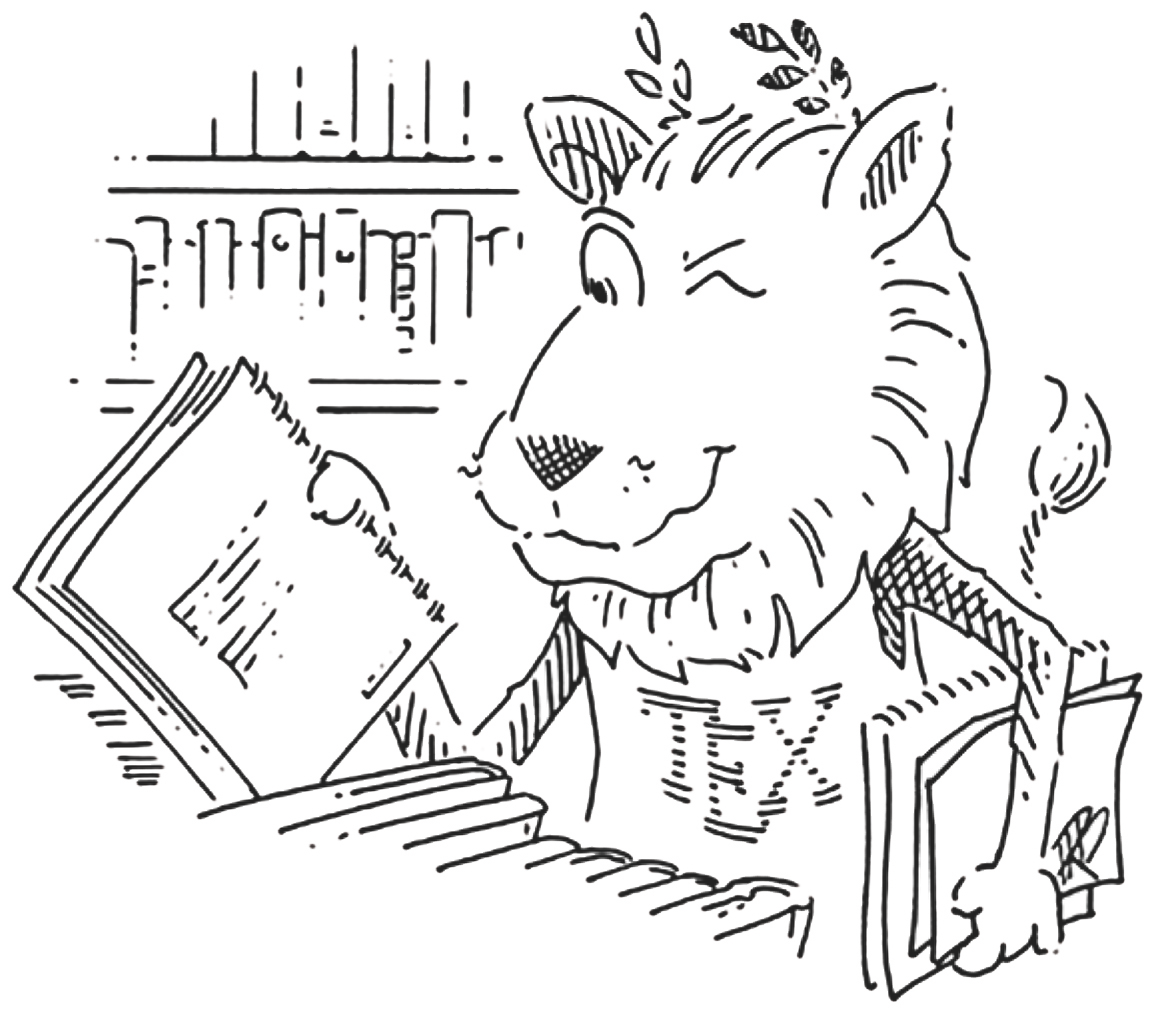
\includegraphics[width=0.75\textwidth]{images/lion.png}
\vspace{3ex}

{\large \emph{Le seul livre sur \LaTeX sans une seule équation !}}

\vspace{28ex}



{\small Publié sous licence \href{http://creativecommons.org/licenses/by-sa/3.0/fr/}{Creative Commons France 3.0 - Paternité - Partage à l'Identique}}
\end{center}
\newpage
\else
% La couv
\newgeometry{right=0cm,top=0cm,bottom=0cm,left=0cm}
\thispagestyle{empty}
\noindent
\includegraphics{images/couv.jpg}
\restoregeometry

% Mention légale
\null\vfill

{\small Version papier : \url{http://www.atramenta.net/books/latex-sciences-humaines/79}

Mise en page : Maïeul Rouquette

Couverture : Laura Pigeon

Éditeur : \href{http://www.atramenta.fr}{Atramenta}

Publié sous licence \href{http://creativecommons.org/licenses/by-sa/3.0/fr/}{Creative Commons France 3.0 - Paternité - Partage à l'Identique}}
\thispagestyle{empty}

\fi

\def\epi{Du \LaTeX sed \TeX}
\def\episource{Proverbe Latin}

\phantomsection\part*{Avant-propos\addcontentsline{toc}{part}{Avant-propos}}
\pdfbookmark[0]{Remerciements et détails techniques}{}
\phantomsection\addcontentsline{toc}{section}{Remerciement}\section*{Remerciement}\thispagestyle{plain}

Nombreuses sont les personnes à remercier pour leur participation à ce projet. Tout d'abord Brendan Chabannes et ma sœur Enimie qui ont accepté d'écrire plusieurs passages, ainsi que Laura Pigeon pour avoir mis en page la première et la quatrième de couverture.

Christophe Masutti m'a incité à écrire ce livre et je ne me serais pas lancé dans cette rédaction sans ses encouragements. Ma reconnaissance va également à mon directeur de mémoire, Rémi Gounelle, qui a aimablement accepté de prendre sur son temps décanal pour discuter de ce projet.

Deux amis astronomes sont à mentionner : Benjamin pour m'avoir fait découvrir  \LaTeX et Yannick pour m'avoir convaincu, sans le savoir, de l'utiliser pour mon mémoire, au cours de l'une de nos nombreuses conversations électroniques.

Il ne faudrait pas que j'oublie Thomas Boitel, mon correspondant chez Atramenta : il m'a fourni ses conseils avisés d'éditeur dans les derniers mois de préparation de cet ouvrage.

Je tiens également à remercier l'ensemble de la communauté \LaTeX sans qui ce livre n'aurait pu exister, faute d'objet. 


\newpage
\phantomsection\addcontentsline{toc}{section}{Au sujet de ce livre}\section*{Au sujet de ce livre}\thispagestyle{plain}

Il va de soi que ce livre a été composé avec \XeLaTeX. Outre les packages dont il traite, j'ai utilisé le package  \package{minted} pour les citations de code ; les packages \package{mdframed} et \package{framed} pour les boîtes colorées.



Ce livre est diffusé sous licence \emph{Creatives Commons - Paternité - Partage des Conditions Initiales à l'Identique 3.0 France}. Sommairement\footnote{Pour les détails, je renvoie au texte intégral de la licence : \url{http://creativecommons.org/licenses/by-sa/3.0/fr/legalcode}.}, cela signifie que vous pouvez le diffuser, le dupliquer, le publier et même le modifier si vous respectez deux conditions:
\begin{enumerate}
\item que vous citiez mon nom\footnote{Et que vous ne portiez  pas atteinte à mes droits moraux.};
\item que vous offriez les mêmes droits aux destinataires de vos diffusions\footnote{Les images de pas et d'éclair servant à indiquer les encarts sont tirées du domaine public et (légèrement) modifiées par mes soins. Elles ne sont donc pas affectées par ces règles. Voir \url{http://www.openclipart.org/detail/154855/green-steps-by-netalloy} et \url{http://thenounproject.com/noun/high-voltage/}. L'image de couverture est de Duane  Bibby, avec une légère modification. Voir \url{http://www.ctan.org/lion.html}.}.
\end{enumerate}

Bien sûr, si vous souhaitez me soutenir, vous pouvez acheter cet ouvrage en version papier, ou simplement m'envoyer un petit mot --- vous trouverez aisément comment me contacter sur Internet.

Si vous souhaitez améliorer cette œuvre, soyez le bienvenu. Le code est mis à disposition sur GitHub\footnote{À l'adresse \url{https://github.com/maieul/latexhumain}.}, un service fonctionnant à l'aide de l'outil de travail collaboratif Git\renvoi{svn} mais disposant d'une interface d'édition en ligne. 

N'hésitez pas à me demander un accès à l'édition du projet ! 


\chapter[Introduction]{Introduction : intérêt de \LaTeX{} en sciences humaines}

\section{Un manque important}

Ce livre est le fruit d'un an et demi de travail et d'utilisation quotidienne de \LaTeX pour la rédaction de notre mémoire de master. Il vient, à nos yeux,  combler un vide. En effet, si les ouvrages sur \LaTeX sont nombreux, rares sont ceux destinés  spécifiquement aux sciences humaines. 

Si le mot \LaTeX a déjà été entendu par des oreilles humanistes, il évoque --- sauf rares exceptions --- au mieux un outil pour les sciences dites dures, au pire la sève d'un arbre ou un plastique aux nombreuses applications. 

Certaines raisons pourraient expliquer ce quasi-vide:
\begin{itemize}
\item Une tendance des chercheurs en sciences humaines à mal connaître ou méconnaître l'outil informatique ;
\item \LaTeX paraît \emph{au premier abord} peu convivial ;
\item Pendant longtemps \LaTeX n'a pas disposé d'outils pour gérer convenablement et simplement une bibliographie selon les normes propres aux sciences humaines : notes de bas de page, distinction entre sources primaires et secondaires, etc. ;
\item Il fut un temps où la gestion des caractères non latins n'était pas des plus aisées en \LaTeX ;
\item Les éditeurs de sciences humaines acceptent rarement des textes formatés en \LaTeX parce que les auteurs les rédigent rarement en \LaTeX parce que les éditeurs les acceptent rarement en \LaTeX\ldots
\end{itemize}

Alors que les chercheurs en sciences humaines sont des spécialistes de l'écrit, durant un temps seuls des logiciels de traitement de texte comme LibreOffice.org ou Microsoft Word ont été utilisés pour la rédaction des travaux universitaires.

Et c'est là un paradoxe : en effet, comme nous allons le voir, ces traitements de texte souffrent de défauts majeurs qui devraient inciter les écrivains à en changer. 

\section{Pourquoi \LaTeX{} ?}

\subsection{Inconvénients des traitements de texte}

Quand vous rédigez dans votre traitement de texte, comme par exemple Microsoft Word ou LibreOffice.org, celui-ci exécute deux actions simultanées :

\begin{itemize}
\item D'une part il stocke dans un fichier la structure logique de votre travail : titres, paragraphes, notes de bas de page etc.
\item D'autre part il vous affiche à l'écran le rendu \enquote{physique} de votre texte (justification, gras, italiques, etc.), tel qu'un lecteur en disposera.
\end{itemize}

Pour cette raison on appelle ce type de logiciel WYSIWYG, ce qui en anglais est l'acronyme de  \textenglish{\emph{What You See Is What You Get}}\footnote{\enquote{Ce que vous voyez est ce que vous produisez}.}. 

Cette combinaison de deux fonctions différentes dans les  traitements de texte entraîne trois conséquences :

\begin{itemize}
\item La nécessité d'afficher en temps réel le rendu physique du texte tout en conservant une vitesse élevée du logiciel a pour conséquence une baisse de la qualité typographique. Par exemple :
	\begin{itemize}
		\item Pour avoir un texte justifié à gauche et à droite, les traitements de texte font varier la taille des espaces entre les mots. Les variations sont parfois considérables, ce qui peut diminuer le confort de lecture. Afin d'éviter ce type d'ennui, les livres classiques coupent les mots en fin de ligne, ce qu'on appelle une césure\footnote{La césure ne se fait toutefois pas n'importe où : elle doit respecter des règles propres à chaque langue.}.
		\item Les blancs situés avant certains signes de ponctuation, comme par exemple les points d'exclamation, sont de  la même taille que les blancs séparant les mots, alors que les règles typographiques classiques prévoient des blancs plus petits.
	\end{itemize}
\item Le fait qu'un même logiciel s'occupe \emph{à la fois} de l'affichage et de la structure du texte incite à confondre les deux\footcite[L'auteur de ces lignes est moins sévère envers les traitements de texte que d'autres LaTeXiens : \cf][]{stupide}  :
	\begin{itemize}
		\item Une telle pratique pousse à se concentrer sur la forme plutôt que sur le fond et la structure\footcite[Toutefois en théorie la formation universitaire en sciences humaines incite à penser \emph{structure et sens d'abord}. Voir un débat sur le blog de l'auteur :][]{structurevsforme}. 
		\item Les rédacteurs n'utilisent pas toujours la possibilité de séparer sens et forme grâce aux styles. Dans ce cas, lorsque l'on désire changer la forme d'un élément logique, comme  le titre d'un chapitre, on doit changer l'ensemble des endroits où cet élément logique est utilisé\footnote{Par exemple, pour une personne  qui n'aurait pas utilisé les styles pour désigner ses titres de chapitre, il faudra sélectionner \emph{l'ensemble des titres de chapitres} puis aller dans les menus de mise en forme, etc.}.
	\end{itemize}

\item Les lourds calculs informatiques nécessaires à la mise en forme en temps réel rendent les traitements de textes particulièrement lents comparativement à d'autres logiciels. Cette lenteur est souvent source d'énervement et de perte de concentration. En outre, ces logiciels exigent bien souvent du matériel récent.
\end{itemize}

Par ailleurs si les traitements de textes récents disposent d'outils de gestion de bibliographie, ceux-ci manquent en général de souplesse ; c'est pourquoi ils sont rarement utilisés\footnote{Il est toutefois possible de passer par des outils externes, tels que EndNote ou Zotero.}. Ainsi, nombreux sont les rédacteurs à écrire  leur bibliographie \enquote{à la main} en tapant directement : Nom de l'Auteur, \emph{Titre}, etc. En cas d'erreur, il faut donc corriger l'ensemble des endroits où l'œuvre est citée.

\subsection{Avantages de \LaTeX{}}

\LaTeX{} permet de résoudre l'ensemble des problèmes des traitements de texte. En effet, il sépare deux étapes : 

\begin{itemize}
\item L'étape de rédaction, qui se passe dans un éditeur de texte. L'auteur frappe son texte et indique par un certain nombre de commandes sa structure (titres, paragraphes, notes de bas de page).
\item L'étape de calcul du rendu final se fait seulement  ensuite : l'auteur  passe son fichier par un compilateur\footnote{Qu'on peut sommairement décrire comme un ensemble de scripts informatiques destinés à produire un objet informatique à partir d'un langage plus facile à lire pour les humains.}, parfois aussi appelé compositeur\footnote{En réalité, le terme \forme{compositeur} est plus correct, du point de vue du vocabulaire informatique, que le terme \forme{compilateur}. Toutefois ce dernier est plus souvent utilisé dans la langue courante.}. Ce dernier programme va lire l'ensemble des commandes du fichier pour produire un nouveau fichier au format PDF\footnote{Historiquement \LaTeX{} produisait un autre format de fichier : DVI. Mais pour notre propos, cela n'a pas d'importance : dans ce livre nous n'utiliserons que la production de PDF.}.
\end{itemize}

Cette séparation permet :
\begin{itemize}
\item Une qualité typographique supérieure :  le compilateur n'ayant pas la contrainte d'un affichage en temps réel, il peut faire des calculs plus lourds : ainsi par exemple \LaTeX{} produit des césures typographiques et non pas des blancs à géométrie variable, et équilibre bien mieux la composition du texte.
\item Une meilleure séparation du sens et de la forme puisque l'auteur donne uniquement des indications de sens.
\end{itemize}

En outre \LaTeX{} possède un système de gestion de la bibliographie extrêmement puissant qui permet à l'auteur de séparer le contenu de sa bibliographie\footnote{Titres, auteurs etc.} de son affichage\footnote{Faut-il mettre des \emph{op. cit.}, et si oui où ? faut-il mettre uniquement les initiales des prénoms ou les prénoms en entier ? etc.}.

Cette séparation entre contenu de la bibliographie et affichage est utile non seulement aux auteurs mais aussi aux éditeurs. En effet, si l'auteur structure correctement sa base de données bibliographique\renvoi{bddbiblio}, l'éditeur peut adapter l'affichage de la bibliographie à ses propres règles : il lui suffit de créer des fichiers de styles bibliographiques suivant une syntaxe simple.

La gestion d'une bibliographie est à la fois l'un des travaux les plus importants en sciences humaines et l'un des plus pénibles, avec de nombreuses sources possibles d'erreurs. Cette simple raison suffit aux yeux de l'auteur à préférer \LaTeX{} à un logiciel de traitement de texte\footnote{L'auteur ainsi que sa sœur se sont décidés à utiliser \LaTeX{} dans le cadre de leurs travaux universitaires, et l'élément déclencheur du choix a été la facilité et la souplesse de la gestion bibliographique.}.

Un autre avantage de \LaTeX{} est la production directe d'un document au format PDF. Lorsque l'on reçoit des documents sous forme numérique, il est bien fréquent qu'à l'ouverture du fichier la mise en page soit perdue, que l'impression soit de mauvaise qualité, ou même qu'il soit tout bonnement impossible d'ouvrir le fichier.

Le \emph{\textenglish{Portable Document Format}} permet d'éviter ces inconvénients. Il s'agit d'un format ouvert, c'est-à-dire que son créateur, la société Adobe, a publié toutes les spécifications nécessaires à la création de logiciels pouvant lire ce format. Par conséquent, il existe de nombreux lecteurs de PDF utilisables sur un grand nombre de systèmes d'exploitation\footnote{Pour un aperçu des lecteurs libres et gratuits disponibles pour votre système d'exploitation, si vous n'en disposez pas déjà d'un, rendez-vous à la page \url{http://pdfreaders.org/index.fr.html} (en français).}.

Le format PDF est conçu pour être lisible de manière universelle. Il embarque en effet dans un même fichier non seulement le texte et les éventuelles images, mais aussi les indications de mise en page et les polices de caractère. Être aussi complet  garantit que celui qui visionnera votre document ou bien le lira sous sa forme imprimée verra exactement ce que vous aviez en tête lorsque vous l'avez composé, ce qui constitue un avantage indéniable sur les formats de fichiers tels que celui de Microsoft Word, par exemple. En outre, vous avez la certitude que le PDF que vous conservez est pérenne. Dans la mesure où chacun est libre de concevoir un logiciel permettant la lecture des PDF et que les spécifications sont librement accessibles, vous avez la garantie de ne pas voir le sort de vos publications dépendre de la bonne volonté d'un vendeur de logiciels au cours des années à venir, ce qui fait du PDF un format de choix pour archiver des publications.

La médaille a hélas son revers: format de fichier lisible universellement, le PDF est fort difficile à modifier confortablement: il n'est pas prévu pour cet usage. C'est pourquoi, si vous souhaitez travailler en collaboration sur un ouvrage en utilisant \LaTeX, il vous faudra travailler différemment\renvoi{principesvn}.

\subsection{Qu'est-ce qu'un éditeur de texte ?}

Nous avons parlé dans les paragraphes précédents de deux types de logiciel, qu'il ne faut pas confondre :
\begin{enumerate}
	\item Les traitements de texte.
	\item Les éditeurs de texte.
\end{enumerate}

Nous avons vu ce qu'étaient les premiers : des logiciels qui s'occupent d'insérer dans un fichier la structure logique d'un texte et de montrer son rendu physique.
Les seconds sont simplement des logiciels qui permettent à une personne d'écrire dans un fichier texte et de placer lui même ses commandes de structuration.
Toutefois les bons éditeurs de texte font plus que cela, ils aident à la rédaction par différents outils :
\begin{itemize}
\item Souvent ils colorient à l'écran les commandes, afin de permettre de mieux les visualiser: c'est ce que l'on appelle la coloration syntaxique.\label{colorationsyntax}
\item Ils proposent des aides pour frapper les commandes les plus fréquentes :  raccourcis clavier,   boutons, etc.
\item Ils offrent parfois un affichage du plan du travail.
\end{itemize}

Certains de ces éditeurs de texte sont généralistes et adaptés à plusieurs langages informatiques\footnote{Par exemple le \LaTeX{} et le HTML, ce dernier étant utilisé pour les sites internet.}. D'autres sont spécialisés dans tel ou tel langage : ils proposent dans ce cas des outils supplémentaires propres au langage de spécialisation. 

Ainsi les éditeurs spécialisés en \LaTeX{} proposent des boutons spécifiques afin de lancer le compilateur \LaTeX{}.

Pour commencer en \LaTeX{} il vous faut donc abandonner votre ancien traitement de texte et choisir un éditeur de texte spécialisé en \LaTeX{} : nous en listons plusieurs en annexe\renvoi{editeurs}.

\section[TeX, LaTeX, XeTeX, XeLaTeX : points communs et différences]{\TeX{}, \LaTeX{}, \XeTeX{} et \XeLaTeX{} : points communs et différences}\label{TeXLaTeX}

Dans ce chapitre nous avons parlé de \LaTeX{}. Le titre de ce livre parle pourtant  de \XeLaTeX{}. Quelle est la différence ? Voici une brève explication historique, très simplifiée\footnote{Le lecteur curieux trouvera aisément de la documentation plus détaillée sur le sujet, sur Internet notamment.}.

\begin{enumerate}
\item En 1977 Donal Knuth invente  \TeX{} qui était un simple compositeur de texte, capable de transformer un texte structuré par des commandes en un texte mis en forme. Avec \TeX{} on pouvait également inventer ses propres commandes.
\item L'utilisation de \TeX{} était relativement complexe. Leslie Lamport a créé un ensemble de commandes \TeX{} pour en simplifier l'usage. Cet ensemble de commandes a permis de former le langage \LaTeX{} et le compilateur associé.
\item Par la suite un compilateur dérivé de \TeX{} a été créé : \XeTeX{}. Il permet deux choses :
\begin{itemize}
	\item Une gestion  de l'ensemble des écritures mondiales, par le biais du jeu de caractères Unicode\renvoi{utf8}.
	\item Une gestion des nouvelles polices de caractères au format OpenType\footnote{Ce type de fonte permet, par exemple, une gestion poussée des ligatures entre les caractères.}, apparues au début des années 2000.

\end{itemize} 
\item Pour pouvoir utiliser les commandes de \LaTeX{} avec \XeTeX{} on a créé \XeLaTeX{}.
\end{enumerate}

On peut résumer les liens entre \TeX{}, \LaTeX{}, \XeTeX{} et \XeLaTeX{} par le schéma~\ref{sch:tex} (p.~\pageref{sch:tex}).

\begin{figure}[ht]
\centering
% Schéma des parentes entres TeX LaTeX XeTeX etc.
\begin{tikzpicture}
	
	% Les textes
	\node[text height=1ex,anchor=mid] (T) at (0,0) 		 	{\TeX} ;
	\node[text height=1ex,anchor=mid]  (X) at (1, -2)	 	 	{\XeTeX};
	\node[text height=1ex,anchor=mid]  (L) at (-1, -2) 		{\LaTeX};
	\node[text height=1ex,anchor=mid]  (XL) at (0,-4)			{\XeLaTeX};
	
	% Les traits
	\draw[->] (T) -- (X.north);
	\draw[->] (T) -- (L.north);
	\draw[->] (L) -- (XL.100);
	\draw[->] (X) -- (XL.80);
\end{tikzpicture}

\caption{Les relations entre \TeX{}, \LaTeX{}, \XeTeX{} et \XeLaTeX{}}\label{sch:tex}
\end{figure} 

Dans  ce livre nous travaillerons sur \XeLaTeX{}. Toutefois comme la plupart de nos propos peuvent s'appliquer indifféremment  à \LaTeX{} et à \XeLaTeX{}, nous emploierons
le terme \forme{\LaTeX{}}, sauf lorsque nous signalerons une spécificité de \XeLaTeX{}.

\begin{plusloins}
Bien que le sujet soit controversé, il semblerait qu'il faille prononcer le  \forme{X} de \TeX{} comme un \forme{χ} grec, car le nom \TeX{} viendrait du mot grec \forme{\textgreek{τέχνη}} : \forme{art, science}. Ainsi prononcerait-on \forme{latek}.
\end{plusloins}


\section{Publics visés par cet ouvrage}

Cet ouvrage vise  trois publics distincts.

Tout d'abord, les étudiants et chercheurs en sciences humaines qui ne sont pas rebutés à l'idée d'apprendre un nouvel outil informatique, qui, s'il leur semblera leur faire perdre du temps au début, leur en fera gagner un précieux  à l'usage.

Ensuite, les éditeurs de revues et de livres en sciences humaines, pour les inciter à prendre en compte \LaTeX dans leurs choix de format de fichier, et pour leur montrer l'avantage de ce format par rapport aux autres. Nous espérons montrer que \LaTeX permet de résoudre nombre de problèmes d'édition, notamment en ce qui concerne les normes bibliographiques, puisqu'il distingue aisément le sens et la forme.

Enfin les utilisateurs de \LaTeX venant des sciences dites \enquote{dures}, pour leur montrer les spécificités éditoriales des sciences humaines et la nécessité d'extensions --- appelées \forme{package} en \LaTeX{} --- adaptées.


\section{Comment lire ce livre}

Cet ouvrage n'est pas un manuel sur \LaTeX{}. Il se veut plutôt une introduction et ne vise donc à présenter que les bases de \LaTeX{}. Une fois celles-ci posées le lecteur-rédacteur devrait être en mesure de comprendre la logique de \LaTeX{} et par la suite être à même de trouver aisément les informations utiles à son projet.

Évidemment, ces bases ne sont pas les mêmes que celles proposées dans d'autres livres d'introduction à \LaTeX{}, généralement orientés vers les sciences dites dures. 
C'est pourquoi vous n'y trouverez pas la manière d'insérer une équation. En revanche nous y détaillons divers éléments abordés souvent trop rapidement dans les autres introductions : ainsi les diverses façons de faire une citation, d'indiquer un changement de langue, la manière d'écrire dans un ou plusieurs alphabets non latins, etc.

Une première partie sera donc consacrée à présenter les principes de fonctionnement de \LaTeX. Le premier chapitre, sous forme de tutoriel, vise à exposer les concepts essentiels. Les autres chapitres, plus formels, décrivent les outils de base et nécessitent d'avoir compris les concepts. En revanche leur ordre de lecture dépend essentiellement des besoins rédactionnels du lecteur. 

Celui-ci pourrait d'ailleurs fort bien commencer par les premiers chapitres de la seconde partie, qui présente les outils de gestion bibliographique en \LaTeX{}, en commençant par la constitution de la base de donnée bibliographique.

Une troisième partie cherche à introduire l'ensemble des outils nécessaires pour faciliter la navigation dans le travail final : sommaire, renvois internes, index.

Une quatrième introduit des outils \LaTeX{} dont l'auteur a jugé qu'ils pouvaient être particulièrement utiles en sciences humaines.

La séparation entre forme et sens étant au cœur de la logique de \LaTeX{}, nous avons jugé important  de n'aborder, sommairement,  les questions de mise en forme qu'en dernière partie\footnote{Exception faite d'un chapitre particulier de la première partie, mais qui aborde d'abord les questions de mise en sens.}.

Le lecteur nous pardonnera de n'avoir pas mis de conclusion, la nature de ce livre ne s'y prêtant pas. Cependant il trouvera un certain nombre d'annexes, comprenant, outre les indispensables index et bibliographies, diverses informations utiles : comment installer et mettre à jour  \LaTeX{}, comment trouver de l'aide, une présentation de quelques logiciels autour de \LaTeX{}, un glossaire, une présentation d'outils utiles pour le travail à plusieurs sur un même projet.

Chaque chapitre de ce livre commence par une courte introduction mentionnant son objet ainsi que les pré-requis à sa compréhension. Deux types d'encart se situent dans le cours du texte : des encarts \enquote{attention}, marqués par des éclairs et dont il est inutile de détailler la signification, et des encarts \enquote{pour aller plus loin}, marqués par des traces de pas et visant à satisfaire la curiosité du lecteur et le plaisir de la digression de l'auteur. Des renvois vers d'autres sections du livre sont indiqués sous la forme (☞\,page, \textbf{chapitre.section.sous-section}).

Les épigrammes en tête de chaque partie n'ayant pas de prétentions scientifiques, le savant tolérera le léger flou quant à leurs provenance, leurs origines n'ayant pas toujours pu être déterminées avec certitude.

On voudra bien enfin nous excuser de ne pas préciser les numéros de page lorsque nous renvoyons à un manuel d'un package de \LaTeX : étant donnée la fréquence avec laquelle certains d'entre eux sont mis à jour, cette information n'aurait guère été pertinente.



\def\epi{Les Sabins \textelp{} commencerent la bataille, qui fut aspre \& dura longuement}
\def\episource{\cite{Sabins}}

\part{Premiers pas avec \LaTeX}
\chapter[Mit XeLaTeX beginnen]{Mit \XeLaTeX{} beginnen}\label{commencer}

\begin{intro}
Wir nehmen an, dass Sie bereits \LaTeX\renvoi{install} und einen auf \LaTeX{} spezialisierten Texteditor\renvoi{logiciels} installiert haben. Siehe im Anhang.

Zunächst ist sicherzustellen, dass das Textverarbeitungsprogramm die Codiereung UTF-8 verwendet.\footnote{Die Einstellung findet sich in der Regel in den Programmeinstellungen, meist in der Rubrik \emph{Dateiformat} oder \emph{Zeichencodierung}: konsultieren Sie gegebenenfalls das Handbuch des Programms.} Wir werden später \renvoi{utf8} auf den Zweck einer solcher Codierung zurückkommen. Im Augenblick genügt es zu wissen, dass diese die Verwendung nicht-lateinischer Zeichen erlaubt.\footnote{Kyrillisch, Griechisch, Sanskrit, Hebräisch, etc. Auch die Verwendung außerirdischer Zeichen ist möglich.}
\end{intro}

\section{Ein erstes Dokument}

Geben Sie in Ihrem Editor den folgenden Code ein\footnote{Wie wir in der Einleitung erläutert haben (p.~\pageref{colorationsyntax}), hat die Kolorierung, die Sie hier sehen, wenn Sie die elektronische Version dieses Buches lesen, eine syntaktische Bedeutung. Machen Sie sich keine Sorgen, wenn sie in Ihrem Editor anders ist. Denken Sie außerdem nicht, dass Ihr kompilierter Text so aussehen wird.} und klicken Sie auf den Knopf zur Kompilation mit \XeLaTeX \footnote{Dessen Position hängt von Ihrem Texteditor ab. Im Moment können Sie sich mit diesem Knopf begnügen. Später werden Sie einige Befehle lernen müssen, doch machen Sie sich keine Sorgen. Alles wird zu erklärt.}:

\begin{attention}
Wenn Sie einen Mac verwenden, sind die für \LaTeX notwendigen Zeichen nicht auf Ihrer Tastatur sichtbar. Wir haben im Anhang angegeben, wie diese eingegeben werden können\renvoi{claviermac}.
\end{attention}
\inputminted{exemples/premierpas/notions/1.tex}

Betrachten Sie das erzeugte PDF. Um die Grundlagen von \LaTeX zu verstehen, werden wir nun zunächst den Code, den Sie kopiert haben, Zeile für Zeile lesen und kommentieren.

\section{Struktur eines \LaTeX-Dokuments}

\subsection{Die Dokumentenklasse}
Die erste Linie \csp{documentclass}\verb|[12pt,a4paper]{book}| bestimmt die Dokumentklasse, in diesem Fall \classe{book}. Eine Klasse beinhaltet eine editorische Entscheidung -- Layout und allgemeine Gliederung des Dokuments. Die Wahl der Klasse beeinflusst unter anderem:

\begin{itemize}
\item Die Anzahl der verfügbaren Überschriftsebenen.
\item Die Seitenränder.
\item Kopf- und Fußzeilen.
\end{itemize}

Es existieren standardmäßig mehrere Dokumentenklassen: etwa \classe{book}, mit der Bücher verfasst werden können; die \classe{article} eignet sich für Aufsätze; \classe{beamer} ist zur Erstellung von Präsentationen vorgesehen. Wir werden uns in dieser Einführung hauptsächlich mit den ersten beiden Klassen beschäftigen, \classe{beamer} aber auch kurz vorstellen\renvoi{beamer}.


Jedes \LaTeX-Dokument beginnt mit der Deklaration der Dokumentenklasse. Die Syntax lautet: \cs{documentclass}\oarg{Optionen}\marg{Klasse}.

\begin{attention}
In diesem Buch dienen Texte in spitzen Klammern (\arg{wie hier}) als Platzhalter und müssen in Ihrer \ext{tex}-Datei durch einen bestimmten Ausdruck ersetzt werden.
\end{attention}

Die Optionen dienen dazu, bestimmte Eigenschaften der Klasse genauer zu bestimmen. In unserem Beispiel wählen wir 12~pt als Größe der Schriftart des Fließtextes und A4 als Papierformat. Mehrere Optionen können angegeben und durch Kommas getrennt werden.\label{optionsclasse}

Hier einige verfügbare und für Geisteswissenschaften nützliche Optionen:

\begin{description}
\item[10pt] für eine Grundschriftart der Größe 10~pt.
\item[11pt] für eine Grundschriftart der Größe 11~pt.
\item[12pt] für eine Grundschriftart der Größe 12~pt.
\item[onecolumn] für einen einspaltig gesetzten Text. In den erwähnten Klassen ist das der Standard.
\item[twocolumn] für einen zweispaltig gesetzten Text.
\item[oneside] für einseitigen Druck. \label{nbsides}
\item[twoside] für doppelseitigen Druck.\footnote{Bei dieser und der vorherigen Option geht es im Wesentlichen um die Frage der Bindung. Die Option \option{twoside} erzeugt für Vorder- und Rückseiten jeweils unterschiedliche linke und rechte Ränder. Außerdem werden die Seitenzahlen abwechselnd innen und außen gedruckt.}\label{rectoverso}
\end{description}

Wir werden weitere Optionen nach und nach darstellen, nachdem die notwendigen Begriffe angesprochen wurden.

\subsection{Der Aufruf von Packages}

Betrachten wir die beiden folgenden Zeilen: 

\begin{latexcode*}{linenos,firstnumber=2}
\usepackage{fontspec}
\usepackage{polyglossia}
\end{latexcode*}

Es handelt sich, wie Sie erahnen können, um den Aufruf von Packages.\footnote{Wir haben uns bewusst entschlossen, diesen Begriff nicht zu übersetzen, um Verwechslungen vorzubeugen.} Ein Package ist eine Sammlung von Dateien, die -- einem Plugin bei Firefox vergleichbar -- weitere Funktionen zu \LaTeX hinzufügen. 

Das erste Package ist \package{fontspec}. Es ist hilfreich für fortschrittliche typographische Anwendungen, besonders um im erzeugten PDF Akzente [disposer] zu können.

Das Paket \package{fontspec} lädt automatisch \package{xunicode}, ohne dass Sie dies zusätzlich angeben müssen. Letzteres erlaubt es, unicode zu erzeugen, das auch UTF-8 genannt wird.\footnote{UTF-8 ist eigentlich nicht identisch mit Unicode, sondern stellt eine Implementierung dessen dar. Aus Gründen der Einfachheit, werden wir beide Begriffe jedoch synonym verwenden.} Daher können wir nicht-lateinische Zeichen\renvoi{utf8} in unserem \ext{tex}-Dokument verwenden.

\begin{plusloins}
Man findet im Internet häufig Hinweise, dass man zur Eingabe von \enquote{ö} den Code \verb|\"{o}| verwendet, wobei andere Sonderzeichen ähnlich eingegeben werden können. 

Dies galt früher, doch es ist bereits seit einiger Zeit nicht mehr hilfreich, diese Befehle zu lernen. Man kann Sonderzeichen ohne Bedenken \enquote{normal} eingeben. 
\end{plusloins}

Das zweite manuell geladene Package \package{polyglossia} ermöglicht, auf einfache Weise ein mehrsprachiges Dokument\renvoi{i18n} zu erzeugen, wobei die nötigen typographischen Anpassungen vorgenommen worden.

Diese drei Packages sind speziell für \XeLaTeX konzipiert: Sie funktionieren nicht mit \renvoi{TeXLaTeX} \LaTeX.

Manche Packages können mit Optionen geladen werden, die ihr Verhalten anpassen. Die Syntax lautet \csp{usepackage}\oarg{options}\marg{package}.

Im Lauf dieses Buchs werden wir verschiedene Packages [aborderons].


\begin{attention}
Im weiteren Verlauf des Buches gehen wir, wenn wir die Funktionen eines Packages beschreiben, davon aus, dass das entsprechende Package zuvor in der Präambel mit dem Befehl \csp{usepackage}\marg{package} geladen wurde.
\end{attention}

\begin{plusloins}
Wenn wir über ein Package sprechen, verweisen wir häufig auf dessen Dokumentation. Man kann diese leicht über das Terminal finden. Wie das genau funktioniert, erklären wir im Anhang \renvoi{manuels}.
\end{plusloins}

\subsection{Französisch als Hauptsprache des Dokuments\label{french}}

Direkt danach bestimmt die Zeile \csp{setmainlanguage}\verb|{french}| Französisch zur Hauptsprache des Dokuments und dass somit bei der Erstellung der Ausgabe die typographischen Gepflogenheiten des Französischen\renvoi{i18n} berücksichtigt werden sollen. Diese Zeile ist für den Compiler nur verständlich, wel wir bereits \package{polyglossia} geladen haben. 

\begin{plusloins}
Vielleicht werden Sie vom Paket \package{babel} hören. Es wird häufig anstelle von \package{polyglossia} verwendet, besonders da es älter ist. Wir haben allerdings beschlossen, uns auf \package{polyglossia} zu beschränken, da wir dieses für die Erstellungen unserer Arbeiten verwendet haben und weil es mehr Funktionen bietet, etwa für Sprachen, die nicht-lateinische Schriften verwenden.

Sie können Informationen über \package{babel} ohne Schwierigkeiten im Internet finden.
\end{plusloins}

\subsection{Der Dokumentenkörper}

Was wir bislang betrachtet haben, der Teil vor \cs{begin}\verb|{document}|, gehört zur sogenannten Präambel des Dokuments.\label{preambule} Diese Informationen erscheinen nicht im erzeugten Dokument. Es handelt sich um Metadaten, die bei dessen Erstellung berücksichtigt werden. Alle Packages, die sie verwenden möchten, müssen in der Präambel geladen werden.

Was sich zwischen den Linien  \cs{begin}\verb|{document}| und \cs{end}\verb|{document}| befindet, stellt den Körper des Dokuments dar, d.h. den eigentlichen Inhalt Ihrer Arbeit.

Nichts, was sich schließlich nach \cs{end}\verb|{document}| befindet, wird vom Compiler berücksichtigt. Sie können hier eingeben, was immer Sie wollen, weswegen wir uns nicht weiter damit befassen.

\subsection{Titel, Autor und Datum: Der Begriff des Befehls}\label{notioncommande}

\begin{latexcode*}{linenos,firstnumber=7}
\title{Un titre d'ouvrage}
\author{Le nom de son auteur}
\date{Une date}
\maketitle
\end{latexcode*}


Les trois premières de ces lignes définissent respectivement le titre (\csp{title}), l'auteur (\csp{author}) et la date (\csp{date}) du travail. En ce qui concerne cette dernière, ne pas l'indiquer revient à indiquer  celle du jour de la compilation, et il faut indiquer \cs{date}\verb|{}| pour qu'aucune date n'apparaisse.

La dernière ligne affiche ces informations. Si votre document est de classe  \classe{book}, alors le compilateur les dispose sur une page à part. S'il est de classe  \classe{article}, il les affiche sans provoquer de saut de page.

On peut déroger à cette règle en passant une option à l'appel de classe\renvoi{optionsclasse}.
\begin{description}
\item[notitlepage] pour ne pas avoir de page de titre spécifique.
\item[titlepage] pour avoir une page de titre spécifique.
\end{description}

Nous pouvons maintenant définir la notion de commande. Une commande  est un bout de code qui est interprété par le compilateur pour effectuer une suite d'opérations, c'est un raccourci d'écriture. 
Ici la commande \csp{maketitle} affiche les informations tel que le titre, la date et l'auteur du travail, informations que le compilateur a apprises grâce aux commandes utilisées au préalable.

Une commande peut prendre des arguments, certains facultatifs, d'autres obligatoires. Ces arguments  modifient son comportement.
\label{syntaxecommande}Une commande s'appelle avec la syntaxe : 
\csp{nom}\oarg{opt1}\oarg{…}\oarg{optn}\marg{obl1}\marg{…}\marg{obln}.

Entre crochets sont indiqués les arguments optionnels, entre accolades les arguments obligatoires. Ces arguments peuvent eux-mêmes contenir des commandes.


L'ordre des arguments dépend de chaque commande, et les arguments optionnels ne sont pas systématiquement avant les arguments obligatoires : ils peuvent être après ou s'intercaler entre. Notez que certaines commandes ne prennent pas d'argument : c'est le cas ici de \cs{maketitle}.

\begin{attention}
À chaque crochet ou accolade ouvert doit correspondre un crochet ou accolade fermé, faute de quoi vous risquez de provoquer une erreur de compilation.
\end{attention}

La grande force de \LaTeX est justement l'utilisation de commandes afin d'éviter la répétition des tâches fréquentes. C'est pourquoi nous apprendrons à définir nos propres commandes\renvoi{creercommandes}.



\subsection{Le corps du texte : la manière de rédiger}

\subsubsection{Analyse de notre exemple}
Regardez maintenant les lignes suivantes et leur résultat à la compilation.


\begin{latexcode*}{linenos,firstnumber=12}
Lorem ipsum dolor sit amet, consectetuer adipiscing elit ?
Morbi commodo ; ipsum sed pharetra gravida !
Nullam sit amet enim. Suspendisse id : velit vitae ligula.
Aliquam erat volutpat.
Sed quis velit. Nulla facilisi. Nulla libero. 

Quisque facilisis erat a dui.
Nam malesuada ornare dolor.
Cras gravida, diam sit amet rhoncus ornare, 
erat      elit consectetuer erat, id egestas pede nibh eget odio.
\end{latexcode*}


Nous pouvons constater plusieurs choses.
\begin{itemize}
\item Une ligne vide produit un changement de paragraphe. Plusieurs lignes vides produisent un seul changement de paragraphe.
\item Un retour à la ligne en revanche se comporte comme une espace\footnote{En matière de typographie, ce terme est féminin.}. C'est une grande différence avec les logiciels WYSIWYG, qui traduisent automatiquement un retour à la ligne  par un saut de paragraphe.
\item Plusieurs espaces à la suite produisent une seule espace. 
\end{itemize}

Vous connaissez donc les règles de bases de la rédaction d'un texte en \LaTeX.

\subsubsection{Allons plus loin}


Nous l'avons dit, \LaTeX produit une mise en page et une typographie plus correctes qu'un logiciel de type WYSIWYG. Il est cependant nécessaire de lui fournir un code correct, afin qu'il puisse déterminer comment typographier.

\LaTeX produit automatiquement  une espace fine devant les signes de ponctuation double,\verb|!:;?| principalement, comme il se doit en bonne typographie fran\c caise\footnote{Une espace fine est une espace plus petite qu'une espace normale.}. Toutefois, nous recommandons d'insérer des espaces dans le fichier \ext{tex} avant ces signes de ponctuation double, pour le confort de lecture.

\begin{attention}
Les espaces avant les signes de ponctuation double sont une spécificité de la typographie française. Il ne sont généralement pas présent dans les autres langues. C'est pourquoi, si vous écrivez dans une autre langue que celle de Molière, il ne faut pas mettre ces espaces. À vous donc de choisir si vous les mettez ou non dans votre fichier source, sachant que \LaTeX les insérera pour vous le cas échéant, mais ne les supprimera pas dans les langues autres que le français.
\end{attention}

En revanche \emph{il est obligatoire de mettre une espace après chaque signe de ponctuation}. Pour ce qui est des points de suspension, il est mieux de ne pas frapper trois points à la suite, mais d'utiliser la commande \csp{ldots} qui espacera correctement les points\footnote{Il est tout à fait possible de configurer l'éditeur de texte pour qu'il remplace automatiquement trois points à la suite par cette commande.}.

En ce qui concerne les guillemets, une partie sera consacrée plus tard à l'art et la manière de faire des citations\renvoi{guillemets} en \LaTeX. Nous n'en parlons donc pas maintenant.

Prêtons attention à certaines lettres ligaturées comme  \verb|œ| et  \verb|æ|. À la différence de la plupart des traitements de texte, \LaTeX ne remplace pas automatiquement les suites \verb|oe| et \verb|ae| par \verb|œ| ou \verb|æ|. Il faut donc frapper soi-même ces caractères, ou configurer son éditeur pour qu'il effectue ce remplacement.

Signalons également trois types de tirets\label{tirets} :
\begin{enumerate}
\item \verb|-| qui produit un tiret simple (-), utilisé pour les mots composés ;
\item \verb|--| qui produit un tiret demi-cadratin (--), en théorie à utiliser pour séparer une plage de nombres ;
\item \verb|---| qui produit un tiret cadratin (---), pour des incises\footnote{Certains éditeurs préfèrent utiliser des tirets demi-cadratins.}.
\end{enumerate}
 
Enfin, il est parfois utile d'insérer une espace insécable, pour éviter que deux mots se trouvent séparés par un retour à la ligne, par exemple entre un nom de souverain et son numéro de règne : \enquote{Jean~\textsc{xxiii}}.  L'espace insécable est produit par le caractère \verb|~|.



Par ailleurs, comme vous avez pu le constater, \LaTeX interprète de manière spécifique un certain nombre de caractères : \verb|\{}~|, à quoi nous ajoutons \verb|%_&$#^|\footnote{Nous ne verrons pas l'utilité \LaTeX  de tout ces caractères, certains servant essentiellement à rédiger des formules mathématiques.}.

Comment faire si nous désirons afficher un de ces caractères ? Il faut les faire précéder du caractère~\verb|\|. Ainsi pour insérer le caractère \verb|%|, il faut écrire \verb|\%|. 

Trois exceptions toutefois :
\begin{description}
\item[\textbackslash] qui s'insère avec la commande \csp{textbackslash} ;
\item[\textasciitilde] qui s'insère avec la commande \csp{textasciitilde} ; 
\item[\textasciicircum] qui s'insère avec la commande \csp{textasciicircum}. 
\end{description} 
\subsection{Un commentaire}

La ligne suivante est : 
\begin{latexcode*}{linenos,firstnumber=22}
%La fin du document
\end{latexcode*}

Il existe en \LaTeX une règle simple : tout ce qui se trouve à droite d'un signe \verb|%| est un commentaire.
C'est-à-dire qu'il n'est pas interprété par le compilateur et n'apparaît donc pas dans le document final. 

Nous conseillons de se servir des commentaires pour indiquer les grandes structures du document et pour commenter les commandes que vous créez vous-mêmes\renvoi{creercommandes}. 

Vous pouvez aussi vous en servir, par exemple, pour faire un commentaire à usage personnel ligne à ligne d'un texte que vous traduisez.

En revanche, nous vous déconseillons de l'utiliser pour des notes personnelles lors de la rédaction. Nous vous indiquerons plus loin comment définir une commande  personnalisée afin de générer un fichier qui les affiche, pour une relecture, et une autre qui les masque, pour le document final\renvoi{commentaireredac}.



\subsection{La notion d'environnement }

Nous avons vu jusqu'à maintenant les notions de  package, préambule, commande. 
Il nous reste à en définir une dernière  : celle d'environnement .

Un environnement  est une portion de document ayant une signification spécifique et qui par conséquent subit un traitement spécifique. Par exemple, pour indiquer une citation, une liste, etc. Nous découvrirons au fur et à mesure  des environnements. 


On marque le début d'un environnement  \arg{nom} par \csp{begin}\marg{nom} et on le termine \csp{end}\marg{nom}.




Dans la classe \classe{article} il existe un environnement utile : \enviro{abstract}. On place dans cet environnement un résumé de l'article :

\begin{latexcode}
\begin{abstract}
Hier schreiben wir eine Zusammenfassung des Artikels. 
\end{abstract}
\end{latexcode}


Il est possible d'imbriquer des environnements :

\begin{latexcode}
\begin{1}
blabla blab
\begin{2}
blabl blab
\end{2}
blabl
\end{1}
\end{latexcode}


En revanche il n'est pas possible de superposer des environnements : ainsi le code suivant ne fonctionne pas et produit une erreur lors de la compilation.


\begin{latexcode}
\begin{1}
blabla blab
\begin{2}
blabl blab
\end{1}
blabl
\end{2}
\end{latexcode}

\subsection{Schluss}

Sie haben nun bereits die grundlegenden Begriffe und Konzepte von \LaTeX kennengelernt. Für den Moment erscheint das sicherlich etwas verwirrend, aber im weiteren Verlauf Ihrer Lektüre werden Sie besser verstehen\ldots\footnote{Zumindest hoffen wir das!}


 \chapter{Structurer son travail}
\begin{intro}
Après avoir découvert les bases de \LaTeX{}, apprenons la manière de structurer son travail.
\end{intro}

\section{Différents niveaux de titres}\label{niveautitre}

\LaTeX{} propose par défaut six ou sept niveaux de titres, selon la classe choisie.
Pour introduire un titre dans \LaTeX{} --- en dehors du titre du travail --- il suffit d'utiliser une commande de titre qui possède la syntaxe suivante: \csp{\meta{titre}}\oarg{titre court}\marg{titre long}.

Le titre court est facultatif, comme l'indique le fait qu'il soit entre crochets\renvoi{syntaxecommande}. Il sert pour la table des matières\renvoi{toc} et, éventuellement, pour les en-têtes des pages\renvoi{entete}.

Évidemment \csp{\meta{titre}} doit être remplacé par le type de titre. Voici les niveaux de titre disponibles, du plus général au plus détaillé. Plus un titre se trouve haut dans la hiérarchie, plus son numéro de niveau est faible.



     \begin{longtable}{|l||l|l|}
    \hline     
     \headlongtable{Commande}                & \headlongtable{Sens}                         & \headlongtable{Numéro de niveau}     \\
     \hline
    \endhead
    \hline
    \endfoot
     \csp{part}            & Titre de partie             & -1     \\
     \csp{chapter}         & Titre de chapitre         & 0           \\
    \csp{section}            & Titre de section          & 1            \\
    \csp{subsection}        & Titre de sous-section     & 2            \\
    \csp{subsubsection}    & Titre de sous-sous-section& 3            \\
    \csp{paragraph}        & Titre de paragraphe         &4            \\

    \csp{subparagraph}        & Titre de sous-paragraphe     & 5            \\
    \end{longtable}



Quelques remarques importantes :
\begin{itemize}
\item Le niveau \cs{chapter} n'existe que dans la classe \classe{book} ;
\item Chaque niveau de titre se voit attribuer un numéro. Ce numéro sert lors de l'affichage de la table des matières pour définir sa profondeur.\label{numeroniveau}\renvoi{tocdepth}
\item Les niveaux dont les numéros sont inférieurs à 1 provoquent un changement de page.
\item Les niveaux dont les numéros sont supérieurs à 3 ne provoquent pas de changement de paragraphe. Les titres sont positionnés en \enquote{lettrine}.
\end{itemize}

\subsection{Des titres non numérotés}\label{titresansnumero}
Par défaut, tous les titres sont automatiquement numérotés\footnote{Nous verrons plus loin comment changer la numérotation\renvoi{apparencecompteur}.}. Il est possible d'obtenir un titre non numéroté, en faisant suivre le nom de la commande d'un astérisque : \csp{chapter*}\marg{Un chapitre non numéroté}.


Toutefois un titre non numéroté ne sera pas ajouté à la table des matières\renvoi{toc}. 

Pour contourner ce problème, il faut utiliser la commande :

\csp{addcontentsline}\verb|{toc}|\marg{1}\marg{2}, où : \label{addcontentsline}

\begin{description}
    \item[\arg{1}] est le type de titre ;
    \item[\arg{2}] est le texte du titre ;
\end{description}

Un exemple sera plus parlant :


\begin{latexcode}
\addcontentsline{toc}{chapter}{Introduction}
\chapter*{Introduction}
\end{latexcode}


\begin{plusloins}
Le lecteur alerte se demandera sans doute pourquoi il est nécessaire de mettre \verb|toc| comme premier argument. Cela correspond à l'extension du fichier qui contiendra la table des matières : nous renvoyons au chapitre dédié à ce sujet\renvoi{toc}.
\end{plusloins}

\section{Structurer ses fichiers}\label{inclusion}

Jusqu'à maintenant, vous aviez tout mis dans un seul fichier. Une fonctionnalité intéressante de \LaTeX{} est la possibilité d'appeler dans un fichier d'autres fichiers, pour ainsi séparer son travail en plusieurs fichiers, chacun contenant une partie seulement du document final.

Par exemple, il est possible de faire un fichier par chapitre d'un mémoire, ou encore  par texte cité dans un exemplier. Seul un fichier \enquote{père} est compilé, ce document appelle des fichiers \enquote{fils}.

Pourquoi procéder ainsi ?
\begin{itemize}
\item Pour pouvoir changer plus aisément l'ordre des parties. 
\item Pour pouvoir \enquote{recycler} plus facilement certaines parties.
\item Pour pouvoir compiler seulement certaines parties.
\end{itemize}

Concrètement, comment fait-on ?
\begin{enumerate}
\item Le fichier \enquote{père} doit systématiquement commencer par un appel de classe, et contenir \cs{begin}\verb|{document}| et \cs{end}\verb|{document}|.
\item Les fichiers \enquote{fils} ne doivent contenir aucun appel de classe, ni les commandes \cs{begin}\verb|{document}| et \cs{end}\verb|{document}|.
\item Ils sont inclus dans le fichier \enquote{père} par l'une des commandes suivantes :
\begin{itemize}
    \item \csp{include}\marg{chemin-du-fichier}, qui entraîne systématiquement un saut de page.
    \item \csp{input}\marg{chemin-du-fichier}, qui n'entraîne pas de saut de page.\label{input}
\end{itemize}
\end{enumerate}

La commande \cs{input}, contrairement à \cs{include}, peut aussi être  appelée dans un fichier \enquote{fils}, voire dans un fichier \enquote{petit-fils} etc.

Nous conseillons de mettre l'ensemble des appels à des packages dans un fichier à part. Ainsi, vous pouvez disposer d'un jeu de packages pour tout vos documents : il suffit d'appeler à chaque fois ce fichier.


\subsection{Comment indiquer le chemin du fichier}\label{chemin}

La notion de chemin de fichier en informatique renvoie à l'arborescence des dossiers sur un ordinateur.

En \LaTeX{}, le chemin du fichier se compte à partir du fichier \enquote{père}, celui qui est compilé, y compris lorsqu'on procède à une inclusion dans un fichier \enquote{fils}.

On indique le chemin du fichier en séparant chaque dossiers par \verb|/|\footnote{Cette norme s'applique même sous Windows, qui sépare traditionnellement les répertoires par des \texttt{\textbackslash} dans les chemins.}. Ainsi, si nous souhaitons inclure le fichier nommé \verb|c.tex| situé dans le dossier \verb|b|, lui même situé dans le dossier \verb|a|, qui se trouve à côté du fichier \enquote{père}, il faut que nous mettions dans notre fichier \enquote{père} : \cs{input}\verb|{a/b/c}|
ou bien
\cs{include}\verb|{a/b/c}|.

\begin{attention}

Il est déconseillé d'avoir des caractères spéciaux dans le nom des dossiers et des fichiers.
\end{attention}

Nous conseillons de mettre les fichiers \enquote{fils} dans un ou plusieurs sous-dossier.

\section{La classe \classenoidx{book} : structuration globale du document}\index[classe]{book}\label{sectionbook}

La classe \classe{book} propose, en plus des niveaux de titres, une manière de structurer en quatre parties son travail : préambules (avant-propos, sommaire, introductions etc.) ; corps du travail ; appendices ; outils de navigation (index, glossaires, bibliographie, tables des matières,  etc.). 

Chacune de ces parties est indiquée par une commande initiale, respectivement : \cs{frontmatter} ; \cs{mainmatter} ; \cs{appendix}\footnote{Cette commande existe aussi dans la classe \classe{article}.}; \cs{backmatter}.

Cette structuration en parties globales a un impact sur la présentation des numéros de page (romains ou arabes) et sur la numérotation des titres.

Ainsi, par défaut : \begin{description}
\item[\csp{frontmatter}] donne des titres non numérotés mais présents dans la table des matières. En outre les numéros de pages sont en chiffres romains minuscules. 
\item[\csp{mainmatter}] donne des titres numérotés. La numérotation des pages est réinitialisée et est en chiffre arabe.
\item[\csp{appendix}] affiche les numéros de chapitres sous forme de lettres majuscules. Le texte \forme{chapitre} est remplacé par \forme{appendice}.
\item[\csp{backmatter}] supprime les numéros de chapitres tout en présentant les chapitres dans la table des matières.
\end{description}


\chapter{Gérer les langues avec \packagenoidx{Xunicode} et \packagenoidx{Polyglossia}}\index[pkg]{xunicode}\index[pkg]{polyglossia}\label{i18n}

\begin{intro}
    Dans ce chapitre nous verrons la manière de signaler à \LaTeX les changements de langue, ainsi que les méthodes pour écrire en caractères non latins.
\end{intro}

\section{Indiquer les changements de langue}

\subsection{Pourquoi indiquer les changements de langue ?}

Voici les principales raisons :
\begin{enumerate}
\item Chaque langue  a ses propres règles typographiques (espacement avant et/ou après les signes de ponctuation, par exemple). Indiquer la langue courante permet donc à \LaTeX d'adapter sa typographie.
\item Chaque langue a ses propres règles de césure des mots : indiquer la langue permet d'avoir une césure correcte.
\end{enumerate}


\subsection{Commandes et environnements de changement de langue}

\subsubsection{Langue principale et langues secondaires}

Nous avons vu que dans le préambule on indiquait  le français comme langue principale  par la commande : \cs{setmainlanguage}\verb|{french}|\renvoi{french}.




Évidemment on pourrait indiquer une autre langue :  par exemple si vous écrivez votre travail en grec :
\cs{setmainlanguage}\verb|{greek}|.


On pourrait même préciser qu'il s'agit du grec ancien\footnote{L'auteur de ces lignes aime retarder de quelques mondialisations, c'est pourquoi il préfère le grec ancien à l'anglais.} : 

\begin{latexcode}
\setmainlanguage[variant=ancient]{greek}
\end{latexcode}


On trouve une liste des langues disponibles et de leurs variantes dans la documentation de \package{polyglossia}\footcite{polyglossia}. Dans le cas où votre langue n'est pas disponible, trois solutions s'offrent à vous :
\begin{itemize}
\item regardez si le package \package{babel} ne peut rien faire pour vous;
\item écrivez à l'auteur\footnote{Du package, pas de ces lignes.} en lui présentant le nom de la langue et ses règles typographiques et de césure et demandez lui gentiment d'ajouter une langue à \package{polyglossia};
\item ne respectez pas les bonnes raisons d'indiquer les changements de langue.
\end{itemize}

Pour pouvoir indiquer des changements de langue, il faut déclarer dans le préambule les langues secondaires : 
\csp{setotherlanguage}\oarg{options}\marg{codelang}, où \arg{codelang} est remplacé par le code de la langue, par exemple \contenuarg{greek}.

Les options sont principalement les variantes, mais il peut également s'agir d'options d'affichage des nombres ou des dates : voir le manuel de \package{polyglossia}\footcite{polyglossia_options}.

\subsection{Indiquer un changement de langue}\label{changerlang}

Il existe deux manières d'indiquer un changement de langue.

\subsubsection{Par une commande}

On peut le faire par une commande 
\csp{text\meta{codelang}}\oarg{options}\marg{texte dans une
autre langue} par exemple\footnote{\bibleverse{Jn}(1:1).} : 

\begin{latexcode}
\textgreek[variant=ancient]{Ἐν ἀρχῇ ἦν ὁ λόγος}
\end{latexcode}

\subsubsection{Par un environnement}

Pour des textes plus longs, il peut être intéressant d'utiliser plutôt un environnement \enviro{\meta{codelang}}:

\begin{latexcode}
\begin[variant=ancient]{greek}
Ἐν ἀρχῇ ἦν ὁ λόγος, 
καὶ ὁ λόγος ἦν πρὸς τὸν θεόν,
καὶ θεὸς ἦν ὁ λόγος.
\end{greek}
\end{latexcode}

\subsection{Le problème du latin}\label{redefinirlatin}

Dans le package \package{polyglossia} le latin suit la typographie anglaise. Ainsi le francophone aura quelques soucis s'il désire des espaces avant les signes typographiques doubles dans un environnement \enviro{latin} ou dans une commande \csp{textlatin}.
Pourtant il pourrait vouloir utiliser cet environnement ou cette commande, afin d'avoir un respect des césures latines.

Pour ce faire, il devra redéfinir dans le préambule l'environnement \enviro{latin} par le code suivant :

\begin{latexcode}
\renewenvironment{latin}{\begin{hyphenrules}{latin}}%
{\end{hyphenrules}}
\end{latexcode}

\begin{plusloins}
La commande \csp{renewenvironment} redéfinit un environnement, dans le cas présent \enviro{latin}. Le deuxième argument de la commande indique ce qui se passe lorsque l'on ouvre l'environnement, le troisième argument ce qui se produit lorsqu'on l'on ferme l'environnement. L'environnement \enviro{hyphenrules} indique un changement des règles de césure.
\end{plusloins}


\section{Saisir des textes en caractères non latins}\label{utf8}

Ce que nous allons expliquer maintenant n'a en réalité pas grand chose à voir avec \LaTeX. Il s'agit en fait d'un problème plus général à l'informatique : comment écrire dans des caractères non latins ? Nous allons ici expliquer la mauvaise méthode, puis la bonne méthode.

Nous commencerons par un peu d'explications techniques très simplifiées : que les puristes nous pardonnent.

\subsection{Les jeux de caractères : ou comment se servir de nombres pour autre chose que des mathématiques}

Au départ, un ordinateur ne manipule que des nombres. Mais les ordinateurs servant aux humains, ceux-ci leurs ont appris à \enquote{stocker} des caractères, en associant des lettres à des nombres.

Cependant les premiers ordinateurs ayant été développés par des Anglo-Saxons, on n'a  attribué des nombres qu'à  127~caractères, ce qui suffisait largement pour écrire en anglais et ajouter des caractères spécifiques, comme les accolades informatiques\footnote{Celles dont vous vous servez pour les commandes \LaTeX.}.  Le jeu de caractères connu sous le doux nom d'ASCII\footnote{\emph{\textenglish{American Standard Code for Information Interchange.}}} a ainsi vu le jour.

Un jour d'autres peuples que les Anglo-Saxons ont voulu écrire avec un ordinateur et ont souhaité frapper leurs propres caractères. Par exemple les Européens occidentaux ont voulu taper des accents, des cédilles, des trémas et autres joyeusetés. On a donc créé un nouveau système de codage pour représenter les caractères latins occidentaux, en attribuant des nombres à d'autres caractères. On a ainsi formé le jeu de caractères  ISO-8859-1. 

D'autres ont voulu pouvoir frapper dans leur alphabet, et c'est ainsi que furent inventés des jeux de caractères comme ISO-8859-5 pour le cyrillique. En outre certaines entreprises inventèrent leurs propres manières de stocker des caractères :  ainsi Apple inventa MacRoman et Microsoft Windows-1252\footnote{D'où le fait que pendant longtemps les accents \enquote{sautaient} régulièrement lorsqu'on envoyait un email d'un ordinateur Apple vers un PC sous Windows ou \emph{vice-versa}.}. 

Mais certaines personnes souhaitaient mélanger des caractères de divers alphabets : par exemple écrire tantôt en grec, tantôt en cyrillique, tantôt en caractères latins. Comment faire ? Pendant longtemps,la technique utilisée\footnote{Qui malheureusement est encore pratiquée, voir apprise, par des personnes peu au courant des évolutions informatiques.} consistait à écrire dans un jeu de caractères donné, typiquement ISO-8859-1, mais en utilisant une police qui affichait le texte dans un autre alphabet. 

Par exemple, pour écrire le caractère grec \enquote{α} on écrivait le caractère latin \enquote{a} et on le faisait afficher dans la police SPIonic. Cette méthode posait --- et pose encore --- de nombreux problèmes :
\begin{itemize}
\item elle nécessitait que la police soit présente sur toutes les machines de travail;
\item ne stockant pas l'information exacte sur le caractère, puisqu'elle utilise un code pour désigner autre chose que ce qu'il devait désigner, elle ne permettait pas  de faire aisément des recherches;
\item avec \LaTeX, étant donné que nous ne sommes pas dans un système WYSIWIG, elle rendait la rédaction et la relecture extrêmement pénible;
\item elle était un non-sens informatique et logique. 
\end{itemize}

Une métaphore simple explique le problème : supposons que vous vouliez une maison en brique rouge. Que diriez-vous si votre entreprise de maçonnerie vous posait du parpaing, puis le peignait en rouge pour faire croire que c'est de la brique ? Voilà le problème fondamental de cette méthode : elle fait prendre du parpaing (la lettre \enquote{a}) pour de la brique (la lettre \enquote{α}) en se servant d'une peinture (la police de caractères).

Heureusement petit à petit une solution a émergé : elle a consisté à inventer un jeu de caractère qui puisse stocker tous les caractères présents sur la terre, y compris dans le passé, tout en laissant de la place pour les caractères des civilisations extra-terrestres qu'un jour, éventuellement, nous rencontrerions. Ce jeu de caractère s'appelle \emph{Unicode}.

Avec ce jeu de caractères, il est donc possible de mélanger allègrement de l'arabe, du vietnamien, de l'hébreu et du cyrillique dans un même fichier. Toutefois, histoire de compliquer les choses, plusieurs implémentations de ces jeux de caractères ont été inventées, chacune présentant des avantages et des inconvénient divers\footnote{Par exemple sur le volume des fichiers et les temps de recherche.}. La plus courante de ces implémentations est UTF-8.

C'est celle que vous utilisez depuis que vous lisez ce livre, si du moins vous avez lu le chapitre~\ref{commencer}.

En un mot : Unicode dans sa variante UTF-8 est aujourd'hui la meilleure méthode pour écrire des fichiers mêlant plusieurs familles de caractères\footnote{L'auteur pense même que, étant donné la baisse des coûts de stockages et de transferts, on ne devrait plus utiliser que ce jeu de caractères, ce qui aurait pour mérite de permettre bien plus facilement à tous les peuples de s'exprimer dans leur langue. Malheureusement son expérience personnelle lui prouve que cela n'est pas encore toujours le cas.}.

\begin{attention}
Le système Unicode est plus complexe que nous ne l'avons expliqué. Ainsi, certains caractères composés peuvent être encodés de plusieurs manières. Prenons par exemple le caractère grec \enquote{alpha avec iota souscrit} (ᾳ). Il peut être encodé :
\begin{itemize}
	\item Par le caractère \enquote{\textenglish{greek small letter alpha with ypogegrammeni}} (\verb|U+1FB3|).
	\item Par le caractère \enquote{\textenglish{greek small letter alpha}} (\verb|U+03B1|) suivi du caractère \enquote{\textenglish{combining greek ypogegrammeni}} (\verb|U+0345|)\footnote{On note les numéros des caractères unicodes sous la forme U+nombre hexadécimal.}. 
\end{itemize}

En théorie, les deux polices de caractères doivent afficher le même résultat avec ces deux encodages. En pratique, il n'en va pas toujours ainsi\footcite[Pour des exemples et plus d'explication, voir :][]{normalisation_unicode}. C'est pourquoi il est recommandé de mettre le code suivant dans le préambule :
\begin{latexcode}
\XeTeXinputnormalization 1
\end{latexcode}

Ce qui a pour conséquence de faire comme si les caractères étaient encodés selon la première méthode, de manière unitaire.
\end{attention}

\begin{plusloins}
Le lecteur narquois fera remarquer que le même problème  se pose qu'avec la méthode de la police: à savoir que chaque ordinateur de travail devrait implanter Unicode et UTF-8 chez lui. 

L'auteur fera remarquer qu'aujourd'hui tous les ordinateurs possèdent en natif ces possibilités, et qu'il est possible très facilement de l'installer sur des ordinateurs un peu anciens. En outre, avec Unicode on stocke du sens, et non pas de la forme, ce qui permet une plus grande souplesse. 
\end{plusloins}


\subsection{Concrètement}

Fort bien, fort bien, stockons en UTF-8. Mais comment écrit-on en UTF-8 ? Avec les claviers des ordinateurs vendus en Europe occidentale\footnote{Le lecteur militant voudra bien pardonner cet ethnocentrisme.}, nous n'avons pas les caractères grecs à portée de main.

Il faut ici distinguer le support physique : le clavier avec ses touches bien concrètes, et le support logique : le fait que telle touche appuyée donne tel ou tel caractère. 

Pour reprendre notre cas, il suffit de dire à notre ordinateur que la touche A correspond au caractère α. Les ordinateurs récents proposent plusieurs pilotes de clavier en standard\footnote{Sous Macintosh, cela se règle dans les Préférences Systèmes, panneau \enquote{International}, sous Windows cela se règle dans les panneaux de configuration, panneau \enquote{options régionales et linguistiques}; sous Linux, on trouve le réglage dans les Paramètres Systèmes, panneau \enquote{Pays et langue}, onglet \enquote{Agencements}.}. Toutefois ces pilotes de clavier sont généralement destinés aux langues contemporaines, et rarement adaptés aux langues anciennes --- par exemple pour les accents sur le grec\footnote{À l'exception notable de GNU/Linux, qui propose des dispositions de clavier pour le grec polytonique et l'hébreu biblique.}. Heureusement on trouve aisément sur Internet des pilotes de clavier pour d'autres langues\footcites[Pour ce qui concerne le grec ancien, le syriaque, l'hébreu ancien, on pourra utiliser les claviers proposés par Michael Langlois:][]{clavierLanglois}[ou encore, pour le grec, les pilotes de l'École Normale Supérieure][]{clavierENS}.

\begin{plusloins}
Unicode permet de stocker tous les caractères existants sur terre, cependant leurs affichage est confié à une police. Or il n'existe pas de police gérant tous les caractères unicodes. C'est pourquoi il peut être utile d'indiquer une police spécifique pour certaines langues. Nous en parlons dans un chapitre consacré à la gestion des polices\renvoi{policenonlatine}.
\end{plusloins}

\subsection{Et les changements de sens d'écriture ?}

Certaines langues s'écrivent de droite à gauche, d'autres de gauche à droite. On souhaiterait que les alignements de paragraphes, les positions des titres et d'autres éléments correspondent au sens de la langue. 
Comment signaler cela à \LaTeX ? L'indication des changements de langue\renvoi{changerlang} suffit. 

\begin{plusloins}
Pour ce qui concerne l'écriture en boustrophédon, on utilisera le package \package{bidi}. Celui-ci possède des  commandes qui permettent d'indiquer des changements de sens. 
\end{plusloins}

\chapter{Mettre en sens son document (1) : premiers pas}

\begin{intro}
Nous allons maintenant voir comment \emph{mettre en sens} notre document, c'est-à-dire comment poser des balises, des repères, pour marquer le \enquote{relief} sémantique du texte.
\end{intro}

\section{Mettre en forme n'est pas mettre en sens}\label{sensforme}

Lorsque nous lisons un livre, tous les éléments ne sont pas présentés de la même manière : certains sont en gras, d'autres en italique, en souligné, en couleur, etc. 

Tout ceci constitue la \emph{mise en forme} du texte. Si notre livre est bien conçu, ces changements de forme renvoient à des changements de signification : l'italique peut indiquer un titre d'ouvrage ou bien une citation ou une simple insistance, le gras peut indiquer une notion ou une définition ou toute autre signification.

On le voit, la \emph{mise en forme} diffère de la \emph{mise en sens}. Cette dernière est idéalement faite par l'auteur du travail, tandis que l'éditeur s'occupe normalement de la mise en forme et de la mise en page.

C'est d'ailleurs ce qui se passait auparavant quand les auteurs proposaient encore des textes manuscrits à leurs éditeurs : ils indiquaient les éléments à mettre en sens par des signes, mise en sens que l'éditeur transformait en mise en forme\footnote{Dans un traitement de texte de type WYSIWYG, cette distinction se fait normalement à l'aide des styles. Bien souvent malheureusement les utilisateurs ne savent pas s'en servir.}.

Dans \LaTeX, le principe est le même : il existe des commandes de mise en sens qui sont ensuite transformées en commandes de mise en forme. Mieux : on peut définir ses propres commandes de mise en sens. L'intérêt est  évident : pouvoir changer rapidement de mise en forme pour un ensemble de données mises en sens.

Un exemple sera plus parlant. Supposons que nous écrivions un livre d'introduction à l'histoire du christianisme antique. Ce livre cite divers auteurs. Nous souhaitons mettre en valeur ces auteurs, et pour ce faire décidons de les mettre en petites capitales.

Donc, à chaque fois que nous citons un auteur, nous indiquons que nous souhaitons avoir son nom en petites capitales.
Vient le moment où nous imprimons notre livre, et nous nous rendons compte que le choix des petites capitales n'est pas le plus pertinent, mais qu'il vaudrait mieux mettre du gras. Il ne nous reste alors plus qu'à repérer toutes les petites capitales dans notre texte, à vérifier qu'il s'agit bien de petites capitales indiquant un nom d'auteur et à les remplacer par du gras --- travail fastidieux !

En revanche, si au lieu de signaler à chaque occurrence qu'il faut des petites capitales, nous signalons simplement  qu'il s'agit d'un nom d'auteur --- par exemple en écrivant : \cs{auteur}\verb|{Tertullien}| --- nous n'aurons qu'une seule ligne à changer pour indiquer que nous souhaitons avoir les noms d'auteur en gras. Mieux : nous pourrons créer très simplement un index des auteurs\renvoi{indexauteur}.

LaTeX propose quelques commandes simples de mise en sens  : par exemple celles que nous avons vues plus haut pour indiquer les niveaux de titres\renvoi{niveautitre}.

Nous allons ici présenter quelques autres commandes et environnements de mise en sens. Dans le chapitre suivant, nous en indiquerons des spécifiques aux citations\renvoi{citertexte}. Dans un troisième chapitre, nous expliquerons comment créer ses propres commandes\renvoi{creercommandes}, et nous présenterons alors la manière de mettre en forme.

\section{Commandes de mise en sens}

\subsection{Mise en valeur d'un texte}

On peut ponctuellement vouloir mettre en valeur un morceau de son écrit. Pour ce faire il existe la commande \cs{emph}\marg{texte en emphase}.
Exemple :

\begin{latexcode}
On peut se demander si des textes apocryphes 
ont été non seulement \emph{utilisés} mais aussi \emph{lus}
dans la liturgie africaine.
\end{latexcode}

Concrètement cela se traduit par un italique. 

\begin{quotation}
On peut se demander si des textes apocryphes 
ont été non seulement \emph{utilisés} mais aussi \emph{lus} dans la liturgie africaine.
\end{quotation}

Toutefois, à la différence d'une commande qui indiquerait directement de mettre le texte en italique, cette commande pourrait, si on voulait, donner un résultat différent, par exemple mettre en couleur. 

Une autre propriété intéressante est la gestion des imbrications : par défaut une commande \cs{emph} à l'intérieur d'une autre commande \cs{emph} produit un texte en caractères droits.

\subsection{Le paratexte : notes de bas de page et de marge}

\LaTeX propose deux commandes pour indiquer des paratextes\footnote{La question des apparats critiques mise à part, question que nous traiterons plus loin\renvoi{eledmac}.} : pour des notes de bas de page et des notes de marge (la position de ces dernières changeant, quand on est en recto-verso, selon que la page est paire ou impaire). Ces commandes sont, respectivement, \csp{footnote} et \csp{marginpar}.

\begin{latexcode}
Lorem\footnote{Une note de bas de page.} ipsum dolor amat.
Aliquam sagittis\marginpar{Annotation marginale} magna.
\end{latexcode}

\begin{attention}
    On serait tenté d'utiliser cette commande pour citer en note de bas de page une référence bibliographique. Il existe en fait une commande spécifique, que nous étudierons en temps voulu\renvoi{footcite}.
\end{attention}
\begin{attention}
    Certaines mauvaises langues diront qu'il s'agit ici d'une mise en forme et non pas d'une mise en sens. Ils ont partiellement raison, dans la mesure où parfois distinguer la mise en forme de la mise en sens n'est pas évident.
    
    Les personnes vraiment perfectionnistes pourront définir leurs propres commandes pour différencier les différents sens d'une note de marge ou de bas de page.
\end{attention}

\begin{plusloins}
    Certains préfèrent mettre des notes de fin de texte. Bien que nous n'approuvions guère ce choix, nous signalons qu'il est possible d'en produire à l'aide du package \package{endnotes}.
\end{plusloins}

\subsection{Listes}

\LaTeX propose trois types de listes : les listes numérotées, les listes non-numérotées et les listes de description.

\subsubsection{Les listes numérotées}

Une liste numérotée est un environnement \enviro{enumerate}.
Chaque élément de la liste est marqué par la commande \csp{item}.

\begin{latexcode}
\begin{enumerate}
    \item Premier élément
    \item Deuxième élément
    \item Troisième élément
\end{enumerate}
\end{latexcode}

\begin{quotation*}
\begin{enumerate}
    \item Premier élément
    \item Deuxième élément
    \item Troisième élément
\end{enumerate}
\end{quotation*}

\begin{plusloins}
Il existe un package \package{etaremune} proposant l'environnement  \enviro{etaremune} pour obtenir une liste numérotée à l'envers, avec le plus grand numéro en début de liste.

\end{plusloins}
\subsubsection{Les listes non-numérotées}

Une liste non-numérotée est un environnement \enviro{itemize}.
Chaque élément de la liste est marqué par la commande \cs{item}.

\begin{latexcode}
\begin{itemize}
    \item Un élément
    \item Un autre
    \item Encore un autre
\end{itemize}
\end{latexcode}

\begin{quotation*}
\begin{itemize}
    \item Un élément
    \item Un autre
    \item Encore un autre
\end{itemize}
\end{quotation*}

\subsubsection{Les listes de descriptions}

Une liste de descriptions fait correspondre une à une des valeurs. Une telle liste peut être utile pour des lexiques, des glossaires, des chronologies, etc. Pour chaque couple, la première valeur est passée comme argument à la commande \cs{item}. Les listes de définitions sont des environnements \enviro{description}.


\begin{latexcode}
\begin{description}
    \item[325]Concile de Nicée.
    \item[381]Concile de Constantinople.
    \item[431]Concile d'Éphèse.
\end{description}
\end{latexcode}

\begin{quotation*}
\begin{description}
    \item[325]Concile de Nicée.
    \item[381]Concile de Constantinople.
    \item[431]Concile d'Éphèse.
\end{description}
\end{quotation*}

\subsection{Imbrication des listes}

Il est possible d'imbriquer des listes, quels que soient leurs types. On ne peut, par défaut, avoir plus de quatre niveaux d'imbrication.

\begin{latexcode}
\begin{itemize}
    \item Un élément de premier niveau
    \begin{enumerate}
            \item Premier sous élément
            \item Second sous élément
    \end{enumerate}
    \item Un autre élément de premier niveau
\end{itemize}
\end{latexcode}

\begin{quotation*}
\begin{itemize}
    \item Un élément de premier niveau
    \begin{enumerate}
            \item Premier sous élément
            \item Second sous élément
    \end{enumerate}
    \item Un autre élément de premier niveau
\end{itemize}
\end{quotation*}

\begin{plusloins}
On a parfois besoin de personnaliser l'aspect des listes, ou bien encore d'arrêter une numérotation de liste pour la reprendre plus loin. Bertrand Masson a écrit un excellent tutoriel sur la manière d'utiliser le package \package{enumitem} pour arriver à ces fins\footcite{bebert_liste}. 
\end{plusloins}

\chapter{Mettre en sens (2) : l'art de citer en LaTeX}\label{citertexte}

\begin{intro}
Nous évoquerons dans ce chapitre les citations \emph{explicites et textuelles}, c'est-à-dire celles où l'auteur du travail ne se contente pas de renvoyer à une source ou à une étude, mais cite des extraits de cette source.

Une citation peut se faire de deux manières : dans le corps du propos, elle est alors normalement entourée de guillemets, ou bien dans un paragraphe spécifique. Elle est alors généralement présentée avec des marqueurs typographiques particuliers : changement de la taille de police, de la marge etc.

Nous avions vu plus haut qu'il fallait séparer sens et forme\renvoi{sensforme}. Nous allons donc présenter ici les commandes servant à marquer des citations.

\end{intro}
\begin{attention}
Toute citation se doit d'être accompagnée d'une référence, généralement en note de bas de page. Toutefois toute référence n'accompagne pas nécessairement une citation textuelle. C'est pourquoi nous renvoyons pour la gestion des références bibliographiques à la partie qui lui est consacrée.

\end{attention}

\section{Citation dans le corps du texte}\label{guillemets}

Les citations dans le corps d'un texte sont normalement entourées de guillemets français : \verb|«»|. Lorsque qu'on cite un texte qui cite un texte, la citation dans la citation s'entoure de guillemets courbes \verb|“”|. 

\begin{quotation}
    Comme le dit très justement xxx : \enquote{Lorsque yyy déclare \enquote{zzz} il ne déclare rien du tout}.
\end{quotation}

Les claviers disponibles sur nos ordinateurs ne disposent généralement en accès direct que des guillemets anglais\footnote{Une exception notable est la disposition de clavier Bépo.}(\verb|"|). 
La plupart des logiciels WYSIWYG convertissent automatiquement ces guillemets en guillemets français. Rares sont les éditeurs de texte qui le proposent\footnote{C'est d'ailleurs à nos yeux une des raisons qui fait qu'un site internet d'un quotidien national dit \enquote{de référence} n'utilise pas de guillemets français sur sa page d'accueil (à la date du 10 avril 2011), les rédacteurs ne prenant pas le temps de taper les combinaisons complexes de touches nécessaires à la frappe de guillemets français.}. 

En outre, en vertu du principe de séparation du sens et de la forme, évoqué plus haut\renvoi{sensforme}, il est plus pertinent d'utiliser une commande spécifique pour indiquer une citation dans le corps du texte.

Nous allons donc utiliser le package \package{csquotes} qui propose des commandes  pour les citations.



Le package contient une première commande utile : \csp{enquote}\marg{citation}, qui sert pour les citations dans le corps du texte.

\begin{latexcode}
Comme le dit très justement xxx : 
\enquote{Lorsque yyy déclare \enquote{zzz} 
il ne déclare rien du tout}.
\end{latexcode}


\begin{quotation}
Comme le dit très justement xxx : \enquote{Lorsque yyy déclare \enquote{zzz} il ne déclare rien du tout}.
\end{quotation}


Nous constatons que \package{csquotes} s'occupe automatiquement de choisir les bons guillemets. Par défaut on ne peut imbriquer que deux niveaux de citation. Toutefois une option du package permet d'avoir plus de niveaux de citation. Par exemple pour en avoir trois : 

\begin{latexcode}
\usepackage[maxlevel=3]{csquotes}
\end{latexcode}

Le package propose d'autres options et commandes : consultez le manuel\footcite{csquotes}.

\section{Citation dans un bloc séparé}


LaTeX propose en standard trois environnements pour citer dans un bloc séparé.

\subsection{L'environnement \environoidx{quote}}\index[enviro]{quote}

Il est prévu pour des courtes citations d'un paragraphe\footcite[6]{AugustinSermo296}.

\inputminted{exemples/premierpas/citation/rome.tex}

Ce code produit le résultat suivant :

\begin{quote}
Le corps de Pierre gît à Rome, disent les hommes,
le corps de Paul gît à Rome, le corps de Laurent aussi,
les corps d'autres martyrs y gisent,
mais Rome est misérable,
elle est dévastée, affligée, saccagée, incendiée.
\end{quote}


\subsection{L'environnement \environoidx{quotation}}\index[enviro]{quotation}

Il est prévu pour des citations plus longues\footcite{BreveHippone}.



\inputminted{exemples/premierpas/citation/concile.tex}


\begin{quotation}
Que rien exceptées les écritures canoniques ne soit lu en église
sous le nom d’écritures divines.

Les écritures canoniques sont : Genèse, Exode, Lévitique,
Nombres, Deutéronome,
Josué de Noun, Juges, Ruth, 4~livres des règnes,
2~livres des paralipoménes,
Job, psautier, 5~livres de Salomon,
12 livres des prophètes mineurs,
de même Isaïe, Jérémie, Ézechiel, Daniel,
Tobie, Judith, Esther,
2~livres d’Esdras, 2~livres des Maccabées.

Du nouveau testament sont :
4~évangiles, un livre des actes des apôtres,
14~lettres de l’apôtre Paul, 2~de Pierre,
3~de Jean, 1~de Jude, 1~de Jacques,
l’apocalypse de Jean.

Que l’Église d'outre-mer soit consultée
pour la confirmation de ce canon.

De plus, qu'il soit permis de lire les passions des martyrs,
lorsqu'on célèbre leurs anniversaires.
\end{quotation}



\begin{attention}
Le fond gris que vous constatez ici est propre au livre que vous avez sous les yeux. L'environnement \enviro{quotation} standard n'a pas de fond.
\end{attention}

\subsection{L'environnement \environoidx{verse} et le package \packagenoidx{verse}}\index[enviro]{verse}\index[pkg]{verse}


L'environnement  \enviro{verse} permet de citer de façon rapide et simple des poèmes, en gérant notamment le rejet en cas de vers trop long. Chaque vers, à l'exception du dernier, doit se terminer par \verb|\\|. Si le vers est composé de plusieurs strophes, il suffit de sauter une ligne entre chaque strophe. Il ne faut pas mettre \verb|\\| à la fin du dernier vers de chaque strophe.    

Cet environnement est très limité: il ne permet pas de numéroter ni d'indenter les vers, ni encore de rajouter un titre. Si l'on est amené à citer fréquemment des vers, il vaut mieux appeler dans le préambule le package \package{verse}\footcite{verse}. La citation du poème se fait de la même manière.


Avec ce package il faut indiquer \csp{poemlines}\marg{n} pour numéroter les vers cités :  \arg{n} 
définit la fréquence à laquelle les vers sont numérotés. 


Citons pour  exemple un poème entier, dont les vers sont numérotés, de façon assez traditionnelle, une fois sur cinq. En frappant ceci\footcite{demain}:

\inputminted{exemples/premierpas/citation/demain.tex}

on obtient cela :


\begin{verse}
\poemlines{5}
Demain, dès l'aube, à l'heure où blanchit la campagne,\\
Je partirai. Vois-tu, je sais que tu m'attends.\\
J'irai par la forêt, j'irai par la montagne.\\
Je ne puis demeurer loin de toi plus longtemps.

Je marcherai les yeux fixés sur mes pensées,\\
Sans rien voir au dehors, sans entendre aucun bruit,\\
Seul, inconnu, le dos courbé, les mains croisées,\\
Triste, et le jour pour moi sera comme la nuit.

Je ne regarderai ni l'or du soir qui tombe,\\
Ni les voiles au loin descendant vers Harfleur,\\
Et, quand j'arriverai, je mettrai sur ta tombe\\
Un bouquet de houx vert et de bruyère en fleur.

\end{verse}




Si l'on ne cite pas un poème en entier, mais simplement un passage, il faut indiquer à quel vers commence le passage cité, afin que la numérotation des vers que l'on cite soit la bonne.

On utilise la commande \csp{setverselinenums}\marg{premier vers}\marg{premier vers numéroté} : \arg{premier vers} indique le numéro du premier vers que l'on cite, \arg{premier vers numéroté} où doit commencer la numérotation. 

Ainsi, \cs{setverselinenums}\marg{12}\marg{15} indique que l'extrait cité commence par le douzième vers du poème, et que le premier vers numéroté sera le quinzième. 
Avec \cs{setverselinenums}\marg{12}\marg{12}, le premier vers cité sera le premier numéroté.

Ne citant que la troisième strophe, par exemple, il faut frapper :

\inputminted{exemples/premierpas/citation/demainfin.tex}

pour obtenir, correctement numéroté :


\begin{verse}
\poemlines{5}
\setverselinenums{9}{10}


Je ne regarderai ni l'or du soir qui tombe,\\
Ni les voiles au loin descendant vers Harfleur,\\
Et, quand j'arriverai, je mettrai sur ta tombe\\
Un bouquet de houx vert et de bruyère en fleur.

\end{verse}



\begin{plusloins}
Dans la typographie française, il est d'usage de mettre un crochet droit [ au début d'un rejet. Ni l'environnement ni le package \package{verse} ne suivent cette règle. Pour obtenir le crochet droit, il faut charger le package  \package{gmverse} en lui passant l'option \option{squarebr} :

\begin{latexcode}
\usepackage}[squarebr]{gmverse}
\end{latexcode}

Puis insérer, une fois commencé l'environnement \enviro{verse}, la commande \csp{versehangrightsquare}.
\end{plusloins}

Le package \package{verse} permet aussi d'indenter de façon très souple une strophe. On indique avec la commande \csp{indentpattern}\marg{$n_1 n_2 n_x$} l'indentation de chaque vers contenu dans la strophe encadrée à l'intérieur d'un environnement \enviro{patverse}: \arg{$n_1$} correspond au premier vers, \arg{$n_2$} au deuxième et ainsi de suite. Le premier vers n'est jamais indenté, mais il suffit de le faire précéder de \csp{vin}. Avec le code suivant :

\inputminted{exemples/premierpas/citation/apple.tex}

on obtient donc\footcite{EdwardLear} :
  

\begin{verse} 
\poemlines{1}
\indentpattern{010110} 
\begin{patverse} 

\vin There was a young lady of Ryde \\
 Who ate some apples and died.  \\
 The apples fermented \\
 Inside the lamented \\
 And made cider inside her inside. \\
\end{patverse}  
\end{verse}



 
 Si l'on a besoin de répéter une indentation tout le long d'un poème, on remplace \enviro{patverse} par \enviro{patverse*}. Donc pour citer un long extrait en hexamètres dactyliques, plutôt que d'indiquer l'indentation pour chaque vers, il suffit  d'indiquer \cs{indentpattern}\verb|{01}| et d'insérer le poème, en entier,  dans l'environnement \enviro{patverse*} pour avoir un vers sur deux indenté.
 
 
 Le package \package{verse} offre bien d'autres possibilités qui dépassent la simple citation de poésie dans le cours d'un texte. À l'instar d'un autre package, \package{poemscol}, c'est un véritable outil pour éditer de la poésie\footcites(Nous vous renvoyons ici aux manuels de ces packages){verse}{poemscol}. Ni l'un ni l'autre ne permettent en revanche de faire des éditions bilingues: pour cela, il faut utiliser les packages \package{eledmac} et \package{eledpar}\renvoi{eledmac}. 


\section{Citations tronquées et modifiées}

Le package \package{csquotes} propose deux commandes spécifiques pour signaler une citation tronquée ou modifiée.

\subsection{Citation tronquée}

La commande \csp{textelp}\arg{texte} signale un texte tronqué. L'argument \arg{texte} est inséré après la troncature, entre crochets (par défaut) ; pour ne rien insérer, le laisser vide.


\inputminted{exemples/premierpas/citation/conciletronque.tex}


\begin{quotation}
Que rien exceptées les écritures canoniques ne soit lu
en église sous le nom d’écritures divines.
\textelp{Suit la liste des écritures canoniques.}

Que l’Église d'outre-mer soit consultée pour la confirmation
de ce canon.

De plus, qu'il soit permis de lire les passions des martyrs,
lorsqu'on célèbre leurs anniversaires.
\end{quotation}


\begin{plusloins}
On peut décider de la manière dont la troncature et l'ajout sont signalés : consulter le manuel\footcite{csquotes_ellipses}.
\end{plusloins}

\subsection{Citation modifiée}

Pour signaler une modification dans une citation, on utilise  \csp{textins}\marg{texte modifié}.

\inputminted{exemples/premierpas/citation/modif.tex}

\begin{quotation}
Comme le disait très justement xxx :
 \enquote{Lorsque yyy \textins{a déclaré}
\enquote{zzz} il \textins{n'a rien déclaré} du tout}.
\end{quotation}


La commande \csp{textins*} est une variante, servant pour déclarer les changements mineurs nécessaires au nouveau contexte d'énonciation : mise en majuscules, changement de personne etc.

\chapter{Mettre en sens (3) : créer ses propres commandes}\label{creercommandes}

\begin{intro}
Nous avons parlé longuement de l'intérêt de séparer mise en sens et mise en forme\renvoi{sensforme}.
Nous avons indiqué que la meilleure manière pour ce faire était de créer des commandes de mise en sens, qui elles-même appelleraient des commandes de mise en forme.

Voyons maintenant comment créer ces commandes personnalisées.
\end{intro}

\section{Création d'une commande personnalisée}

Nous souhaitons créer une commande personnalisée servant à indiquer que nous parlons d'un auteur : \csp{auteur}\marg{nom}.

Notre commande se décompose en plusieurs parties : son nom, ici \contenuarg{auteur}, et ses arguments, ici un seul : \arg{nom}.

Une commande LaTeX peut prendre jusqu'à neuf~arguments, ce qui est en général bien suffisant. Si nous notons \arg{N} le nombre d'arguments, la syntaxe de la déclaration d'une nouvelle commande est la suivante :
\csp{newcommand}\verb|{\|\arg{nom de la commande}\verb|}|\oarg{N}\marg{code}.

\begin{attention}
    Les noms de commandes ne doivent contenir que des caractères latins non accentués. 
    
    Les noms sont sensibles à la casse : \verb|\a| est différent de \verb|\A|.
\end{attention}
À l'intérieur de la partie \arg{code}, on peut  :
\begin{itemize}
    \item mettre du texte;
    \item utiliser des commandes de mise en forme ou de mise en sens;
    \item appeler les arguments passés en utilisant la syntaxe \verb|#x|, où \verb|x| représente le rang de l'argument.
\end{itemize}

Prenons toujours notre cas d'une commande pour indiquer les noms. Pour le début, nous souhaitons simplement que les noms d'auteur soient suivis d'un astérique (*).

\begin{latexcode}
\newcommand{\auteur}[1]{#1*}
Il est bien connu que \auteur{Tertullien} n'était pas montaniste
mais tertullianiste.
\end{latexcode}

\newcommand{\auteur}[1]{#1*}

Ce qui nous donne :

\begin{quotation}
Il est bien connu que \auteur{Tertullien} n'était pas montaniste mais tertullianiste.
\end{quotation}


\contenuarg{Tertullien} a été passé en premier argument. Il apparaît donc à la place du \#1 de la déclaration de commande.

On pourrait souhaiter passer en second argument des informations complémentaires, comme les dates de vie.

\begin{latexcode}
\newcommand{\auteur}[2]{#1* (#2)}
Il est bien connu que \auteur{Tertullien}{150 ? - 220 ?}
n'était pas montaniste mais tertullianiste.
\end{latexcode}

\renewcommand{\auteur}[2]{#1* (#2)}

\begin{quotation}
Il est bien connu que \auteur{Tertullien}{150 ? - 220 ?}
n'était pas montaniste mais tertullianiste.
\end{quotation}

\begin{plusloins}
Le lecteur attentif se rappellera qu'il existe des commandes avec des arguments optionnels\renvoi{syntaxecommande}. Il souhaitera sans doute en créer lui même.

Si \LaTeX prévoit bien en standard un mécanisme pour permettre cela, celui-ci est  peu souple. 

Nous conseillons donc de se tourner vers les packages \package{xargs} et \package{ifthenelse}\footcites{xargs}{ifthen}.

Mais tout ceci dépasserait le cadre de cet ouvrage.
\end{plusloins}

Fort bien, mais comment faire pour mettre en forme ? Il faut  utiliser une commande de mise en forme à l'intérieur de la déclaration de commande de mise en sens. Par exemple, pour mettre en petites capitales la commande est \cs{textsc}.

\begin{latexcode}
\newcommand{\auteur}[2]{\textsc{#1}* (#2)}
\end{latexcode}

\renewcommand{\auteur}[2]{\textsc{#1}* (#2)}

\begin{quotation}
Il est bien connu que \auteur{Tertullien}{150 ? - 220 ?}
n'était pas montaniste mais tertullianiste.
\end{quotation}

Nous décrirons plus loin un ensemble de commandes de mise en forme\renvoi{mef}.

\begin{attention}
    Si la possibilité de créer ses propres commandes est une grande force de \LaTeX, cela ne fait pas toujours la joie des éditeurs. 
    
    Il est donc recommandé de discuter au préalable avec son éditeur, et surtout de lui indiquer qu'un balisage sous forme de commandes doit, normalement, lui faciliter la tâche.
    
    
    Nous recommandons par ailleurs de regrouper toutes ses déclarations de commandes dans un fichier unique, appelé via une commande \cs{input}\renvoi{input}.
    
    Il est également possible de créer son propre package, pour des commandes utilisées fréquemment dans plusieurs projets\footcite[Ceci dépasserait le cadre de cet ouvrage : je renvoie à d'autres documents. Par exemples][]{creer_sty}.
\end{attention}


\begin{plusloins}\label{commentaireredac}
On peut ainsi très facilement créer une commande \csp{commentaire} servant pour indiquer des commentaires personnels au cours de la rédaction, afin de les avoir sous les yeux lors d'une relecture papier.
Par exemple :

\begin{latexcode}
\newcommand{\commentaire}[1]{\marginpar{#1}}
\end{latexcode}

Lors de l'impression finale, il suffit de changer cette commande par :

\begin{latexcode}
\newcommand{\commentaire}[1]{}
\end{latexcode}
\end{plusloins}

\subsection{Code d'une commande sur plusieurs lignes}\label{commandepourcent}

Jusqu'ici nos commandes étaient relativement simples. Mais il peut arriver que leur code se complexifie. On souhaiterait alors l'avoir sur plusieurs lignes.

C'est tout à fait possible, mais il faut simplement mettre  un signe pourcentage (\%) à la fin de chaque ligne, sous peine d'avoir  des espaces intempestives. Exemple sans  \% :

\begin{latexcode}
\newcommand{\auteur}[2]{
    \textsc{#1}* (#2)
    }
\end{latexcode}

\renewcommand{\auteur}[2]{\underline{ }%
    \textsc{#1}* (#2)\underline{ }%
}

\begin{quotation}
Il est bien connu que \auteur{Tertullien}{150 ? - 220 ?}
n'était pas montaniste mais tertullianiste.
\end{quotation}

On constate une espace en trop avant et une après la mention de l'auteur, que nous avons soulignées pour les besoins de l'explication.
En revanche, si on met des \% :

\begin{latexcode}
\newcommand{\auteur}[2]{%
    \textsc{#1}* (#2)%
    }
\end{latexcode}

\renewcommand{\auteur}[2]{%
    \textsc{#1}* (#2)%
}

\begin{quotation}
Il est bien connu que \auteur{Tertullien}{150 ? - 220 ?}
n'était pas montaniste mais tertullianiste.
\end{quotation}

Il n'y a plus d'espaces intempestives.


\subsection{Étoiler \oldcs{newcommand}}

La création des commandes sous \LaTeX est une fonctionnalité très puissante, mais potentiellement dangereuse. Prenons la commande suivante :

\begin{latexcode}
\newcommand{\auteur}[1]{\textsc{#1}*}
\end{latexcode}

Imaginons que nous l'appelions en oubliant de fermer notre accolade :

\begin{latexcode}
Il est bien connu que \auteur{Tertullien n'était pas montaniste
 mais tertullianiste.
\end{latexcode}

Que va-t-il se passer ? \LaTeX comprend que l'ensemble de la fin du texte est un argument de la commande, ce qui empêche le compilateur de bien fonctionner  et nous n'obtiendrons rien, ou alors un résultat incorrect.

Pour limiter ces soucis, \LaTeX propose de définir des commandes courtes, dont les arguments ne dépassent pas la longueur d'un paragraphe. En cas d'oubli de fermeture de parenthèses, \LaTeX arrête automatiquement l'argument à la fin du paragraphe.

Pour définir ces commandes courtes, il suffit d'utiliser \csp{newcommand*}.

\begin{latexcode}
\newcommand*{\auteur}[1]{\textsc{#1}*}
\end{latexcode}

\subsection{Espace après les commandes sans argument}


Il est possible de définir des commandes sans aucun argument. Prenons une commande personalisée \csp{cf}, qui permet d'obtenir rapidement la forme \forme{\cf}

\begin{latexcode}
\newcommand{\cf}[0]{\emph{cf.}}
\end{latexcode}

Comme notre commande ne prend pas d'argument, il est nécessaire, lorsque nous l'appelons, de la séparer du texte qui suit par une espace, afin que \LaTeX sache où s'arrête la commande : 

\begin{latexcode}
Ceci est très intéressant \cf cela.
\end{latexcode}

Mais  l'espace disparaît lors de la compilation :

\begin{quotation}
Ceci est très intéressant \cf cela.
\end{quotation}

La solution consiste à utiliser dans la définition de commande la commande \csp{xspace} du package éponyme\index[pkg]{xspace}. Elle permet de gérer automatiquement les espaces qui suivent l'appel à une commande, en tenant compte de la typographie.

\begin{latexcode}
\newcommand{\cf}[0]{\emph{cf.}\xspace}
\end{latexcode}

\renewcommand{\cf}[0]{\emph{cf.}\xspace}

\begin{quotation}
Ceci est très intéressant \cf cela.
\end{quotation}

\begin{plusloins}
Le package \package{foreign}\footcite{foreign} propose toute une série de commandes similaires pour indiquer des abréviations ou des expressions étrangères courantes.
\end{plusloins}


\section{Commandes de mise en forme\label{mef}}

Nous listons ici les principales commandes de mise en forme. Pour des besoins avancés, on trouvera aisément de la documentation sur internet. En ce qui concerne les questions d'espacement, un chapitre spécifique leur est dédié\renvoi{espacement}.

\subsection{Taille des caractères}\label{taille}

Il est possible de définir de manière absolue la taille des caractères en indiquant le nombre de points. Toutefois la meilleure méthode est de le définir d'après la taille de base, et d'utiliser les commandes ci-dessous. La taille obtenue dépend de la taille de base définie lors de l'appel au préambule\renvoi{preambule}.

\begin{longtable}{|l|l|}
      \hline
     \headlongtable{Commande}                 &    \headlongtable{Effet}                                 \\
      \hline
     \endhead
    \hline
    \endfoot
     \csp{tiny}             &     \tiny abcdefghijklmnopqrst              \\
     \csp{scriptsize}         &     \scriptsize abcdefghijklmnopqrst          \\
     \csp{footnotesize}     &     \footnotesize abcdefghijklmnopqrst         \\
     \csp{small}            &    \small abcdefghijklmnopqrst             \\
     \csp{normalsize}        &     \normalsize abcdefghijklmnopqrst         \\
     \csp{large}            &    \large abcdefghijklmnopqrst             \\
     \csp{Large}            &     \Large abcdefghijklmnopqrst             \\
     \csp{LARGE}        &     \LARGE abcdefghijklmnopqrst             \\
     \csp{huge}            &     \huge abcdefghijklmnopqrst             \\
     \csp{Huge}            &    \Huge abcdefghijklmnopqrst             \\
\end{longtable}

\label{commandesdetaille}Ces commandes ont toutefois un comportement particulier : ce sont des commandes dites \enquote{à bascule}\renvoi{bascule}. À la différence de la plupart des commandes, elles ne prennent pas d'argument. Elles doivent être utilisées entre accolades, le texte dont la taille change étant inséré après la commande, dans les accolades.

Ainsi :
\begin{latexcode}
{\large Texte plus gros}
\end{latexcode}

Et non pas :

\begin{latexcode}
\large{Texte plus gros}
\end{latexcode}

\subsection{Style de caractères}

Voici une liste non exhaustive de commandes utiles pour personnaliser les styles de caractère.


\begin{longtable}{|l|l|}
    \hline
    \headlongtable{Commande}                & \headlongtable{Effet} \\                                
    \hline
    \endhead
    \hline
    \endfoot
    \csp{textit}            & \textit{Italique}                            \\
    \csp{emph}            & \emph{Texte en emphase}                    \\
    \csp{textbf}            &  \textbf{Gras}                            \\
    \csp{textsc}            & \textsc{Petites capitales}                    \\
    \csp{underline}        & \underline{Souligné}     (à éviter)                \\
    \csp{textsuperscript}    &  \textsuperscript{Exposant}                    \\
    \csp{textsubscript}        & \textsubscript{Indice} (nécessite le package \package{subscript}) \\
\end{longtable}

\subsection{Couleurs}

Les couleurs ne sont pas gérées nativement dans \LaTeX. Il faut passer par le package \package{color} ou le package \package{xcolor} qui proposent tous les deux une commande \csp{textcolor}\marg{nom de la couleur}\marg{texte en couleur}.



La différence tient principalement au nombre de couleurs disponibles par défaut et à la facilité  d'en définir des nouvelles, mais aussi à la possibilité d'appliquer des couleurs à d'autres éléments que le texte. Nous ne présentons ici que le package \package{xcolor}, de manière succincte. Nous renvoyons à la documentation pour des usages avancés\footcite{xcolor}.

\subsubsection{Couleurs standards}
Le package \package{xcolor} propose les couleurs de bases suivantes : 

% Définition de la fonction de modélisation des couleurs
\newcommand{\exemplecouleur}[1]{#1 & \fcolorbox{black}{#1}{~} \\[1pt]}
% Fin de la définition

\begin{longtable}{|l|l|}
    \hline
    \headlongtable{Nom de la couleur}         & \headlongtable{Couleur}                                 \\
    \hline
    \endhead
    \hline
    \endfoot
    \exemplecouleur{black}
    \exemplecouleur{blue}
    \exemplecouleur{brown}
    \exemplecouleur{cyan}
    \exemplecouleur{darkgray}
    \exemplecouleur{gray}
    \exemplecouleur{green}
    \exemplecouleur{lightgray}
    \exemplecouleur{lime}
    \exemplecouleur{magenta}
    \exemplecouleur{olive}
    \exemplecouleur{orange}
    \exemplecouleur{pink}
    \exemplecouleur{purple}
    \exemplecouleur{red}
    \exemplecouleur{teal}
    \exemplecouleur{violet}
    \exemplecouleur{white}
    \exemplecouleur{yellow}
    
\end{longtable}

\subsubsection{Couleurs supplémentaires}

On peut passer les options \option{dvipsnames}, \option{svgnames} ou \option{x11names} lors de l'appel au package \package{xcolor}, chacune fournissant un jeu de couleurs. Ne pouvant lister toutes ces couleurs dans cet ouvrage, nous renvoyons à la documentation de \package{xcolor}\footcite{xcolor_jeu}.

\subsubsection{Définir ses propres couleurs}

Il est possible de définir ses propres couleurs. Il faut  utiliser \csp{definecolor}, selon la syntaxe suivante : 
\cs{definecolor}\marg{nom}\marg{methode}\marg{definition}.


Les couleurs peuvent être définies de plusieurs manières\footnote{On consultera n'importe quel livre scientifique sur les couleurs pour plus de détails. On peut également consulter la documentation du package \package{xcolor}.}. Les deux principales sont\footcite[Il existe aussi la méthode de définition par la longueur d'onde pour les couleurs de l'arc en ciel, par pourcentage de gris pour les différents niveaux de gris, ainsi que par teinte, saturation et luminosité, mais ceci nécessiterait un cours de physique lumineuse. Pour  les personnes intéressées par les détails, consulter][]{xcolor_methode} :
\begin{itemize}
\item La méthode additive en additionnant du rouge, du vert et du bleu (comme sur un écran d'ordinateur).
\item La méthode soustractive en superposant du cyan, du magenta, du jaune et du noir (comme sur une imprimante couleur).
\end{itemize}


Dans les deux cas, il faut  donner une valeur comprise entre 0 (inclus) et 1 (inclus) à chacun des composants\footcite[On pourra trouver une série de code couleur sur le site][]{codecouleur}.

\definecolor{rougebourgogne}{HTML}{6B0D0D}


Prenons par exemple la définition de la couleur \textcolor{rougebourgogne}{rouge bourgogne}\footnote{Avec Anne Sylvestre les auteurs proclament fièrement \enquote{Que Bordeaux me pardonne, j’appartiens au Bourgogne} \parencite{romaneconti}.}.
On peut la définir de la manière suivante en méthode additive :

\begin{latexcode}
\definecolor{rougebourgogne}{rgb}{0.41,0.05,0.05}
\end{latexcode}

Ou bien en méthode soustractive\footnote{Idéalement le choix de  la méthode devrait relever du support de destination. Mais le package \package{xcolors} propose des systèmes de conversion d'une méthode à l'autre.}de la manière suivante :

\begin{latexcode}
\definecolor{rougebourgogne}{cmyk}{0,0.88,0.88,0.58}
\end{latexcode}

Enfin signalons la méthode HTML qui offre l'avantage d'avoir de nombreux sites internet indiquant les codes couleur HTML\footnote{En réalité la méthode HTML est une méthode additive avec des valeurs comprises entre 0 et 255, notées en hexadécimal.}.

La même couleur se définit ainsi :

\begin{latexcode}
\definecolor{rougebourgogne}{HTML}{6B0D0D}
\end{latexcode}





\chapter{Insérer des éléments non textuels}

\begin{intro}
    Dans ce chapitre nous allons examiner comment insérer des éléments qui ne font pas partie du flux du texte : images, graphismes, tableaux de données.
\end{intro}

\section{Insérer des images}

Les images insérables avec \XeLaTeX sont au format JPEG (extension~\ext{jpg}), PNG (extension~\ext{png}) ou PDF (extension~\ext{pdf}). Il est nécessaire d'utiliser le package \package{graphicx}.


L'insertion d'une image se fait ainsi : \csp{includegraphics}\oarg{options}\marg{chemin de l'image}.

Le chemin de l'image s'indique de la même manière que le chemin des fichiers inclus\renvoi{chemin}.
Les principales options, séparables par des virgules,  sont les suivantes\footcite[Pour les autres, on consultera][]{graphicx_options} :

\begin{longtable}{|p{0.2\textwidth}|p{0.45\textwidth}|p{0.2\textwidth}|}
    \hline
    \centering\textbf{Paramètres} & \centering\textbf{Signification} & \centering\textbf{Exemple}    \tabularnewline
    \hline
    \endhead
    \hline
    \endfoot
    angle        & Angle exprimé en degrés. Un nombre positif indique une rotation anti-horaire, un nombre négatif une rotation horaire.     & \verb|angle=90| \\
    height        & Hauteur    & \verb|height=10cm|     \\
    scale        & Redimension proportionnelle & \verb|scale=0.5|\\
    width        & Largeur     & \verb|width=10cm|     \\
\end{longtable}


\begin{plusloins}
Le centimètre n'est pas la seule  unité de mesure disponible en \LaTeX. Nous en parlons en annexe de ce livre\renvoi{unite}.
\end{plusloins}

\begin{plusloins}
Le package \package{graphicx} propose de nombreux outils pour manipuler graphiquement du contenu, textuel ou non. Consultez le manuel\footcite{graphicx}.
\end{plusloins}

\begin{attention}
    Évidemment, il est plus correct d'insérer une légende sous une image. Nous expliquons comment faire plus loin\renvoi{legende}.
\end{attention}

\section{Insérer des graphismes et des schémas}

On peut vouloir insérer divers types de graphismes ou de schémas : graphiques statistiques, arbres généalogiques, \emph{stemma codicum} etc.
Deux solutions s'offrent à nous :
\begin{enumerate}
\item Utiliser un logiciel externe qui exporterait le graphisme dans une image, qu'on insérerait comme n'importe quelle image.
\item Utiliser les possibilités de \LaTeX et du package\package{TikZ}.\label{TikZ}
\end{enumerate}

La première solution paraît de prime abord plus simple, puisqu'elle ne nécessite pas d'apprendre de nouveaux éléments en \LaTeX. Toutefois il faut avec elle gérer plus de fichiers\footnote{Prenons un graphisme généré par un tableur : il faudra conserver la feuille du tableur plus l'image du graphisme généré par celui-ci.}. En outre, les images exportées par ces logiciels étant bien souvent de type bitmap et non pas vectoriel%
\footnote{Il existe deux manières en informatique de coder une image : en codant point par point (image bitmap) ou bien en codant simplement les formes, par exemple des cercles ou des segments (image vectorielle). La première méthode est adaptée à des images complexes, comme les photographies,  la seconde méthode est conseillée pour les images \enquote{simples} telles que les graphismes. La méthode vectorielle possède l'avantage d'offrir une image plus facilement redimensionnable  sans perte de qualité et de permettre aisément la sélection de texte.},
on perd la possibilité de sélectionner dans le PDF généré par \LaTeX les textes, et on risque d'avoir des problèmes de redimensionnement.

Nous allons donc ici vous présenter une des possibilités du package \package{TikZ} : la représentation d'une famille de manuscrits. 

Nous avons choisi cet exemple car il est assez simple, tout en étant fréquent en sciences humaines. Mais \package{TikZ} permet de faire bien plus, comme produire des diagrammes statistiques : nous renvoyons à d'autres ouvrages pour en savoir plus\footnote{Outre le manuel \cite{tikz}, on pourra lire \cites{tikzimpatient}[on pourra également consulter le site][]{tikzexample}.}.
Ce package possède une syntaxe spécifique. 

\begin{attention}
    Bien que le package s'appelle \package{TikZ}, il faut dans le préambule l'appeler \emph{sans majuscules} : \cs{usepackage}\verb+{tikz}+.
 
\end{attention}


Nous disposons de six familles de manuscrits d'un même texte. La  famille A a engendré les familles B, C, D. Les familles E et F pour leur part sont issues de la famille D. 

Le code est le suivant: 
\inputminted{exemples/premierpas/nontextuels/genealogie.tex}

Ce qui donne le résultat de la figure~\ref{figure:genealogie}. Analysons le code :

\begin{figure}[h]
\centering
\begin{tikzpicture}
	\node {A}
		child { node {B}}
		child { node {C}}
		child { node {D}
			 child {
				node{E}
				}
			 child {
				node{F}
				}
			}	
	;
\end{tikzpicture}
\caption{Exemple de \emph{stemma}}
\label{figure:genealogie}
\end{figure}



\begin{description}
\item[Ligne 1] L'environnement \enviro{tikzpicture} est l'environnement utilisé pour insérer une figure TikZ. Il peut recevoir de nombreux arguments pour modifier certains aspects, tels que l'épaisseur par défaut des lignes, la taille du texte, l'orientation du schéma. Nous renvoyons à la documentation.
\item[Ligne 2] Un nœud TikZ, matérialisé  par le commande \csp{node}, est un bloc de texte. On pourrait passer des options à cette commande, afin de modifier certains aspects comme la taille du texte.
\item[Lignes 3 et 4] \verb|child| désigne ici une opération : associer un fils au nœud précédent. Ce fils est lui même un nœud (\verb|node|).
\item[Lignes 5 à 12]Même chose que précédemment, sauf que le nœud D se voit attribuer des fils (E et F). Notez le nombre d'accolades et leurs imbrications : c'est ce qui permet à \package{TikZ} de construire correctement le \emph{stemma}.
\item[Ligne 13] Le point-virgule est obligatoire après chaque commande \package{TikZ} (ici \cs{node}).
\item[Ligne 14] Fin du graphisme \package{TikZ}.
\end{description}

Évidemment un tel code est relativement complexe. C'est pourquoi nous conseillons de le commenter attentivement\footnote{Pour des raisons de place nous ne l'avons pas fait ici.} et de prêter extrêmement attention  aux accolades. Par ailleurs nous recommandons de mettre chaque graphisme \package{TikZ} dans un fichier séparé.


Notre \emph{stemma} est relativement simple : il n'y a pas de contamination. Si cela avait été le cas la construction aurait été plus complexe : on n'aurait pas pu utiliser les opérations de types \verb|child|, en tout cas pas uniquement,  et il aurait fallu positionner précisément les éléments en utilisant un système de coordonnées\footcites[Nous avons publié sur notre site Internet une série d'articles sur les \emph{stemma} avec TikZ :][]{stemma}[on consultera avec profit un article écrit dans la langue de Dante][]{Leal2012a}.

\begin{plusloins}
Le package \package{tikz-qtree}\footcite{tikz-qtree} simplifie la construction de \emph{stemmatta} en proposant une syntaxe simplifiée et des outils pour gérer les cas de contamination.  
\end{plusloins}


\section{Création de tableaux}

\begin{attention}
La création de tableaux en \LaTeX nécessite  une extrême rigueur. 
C'est à nos yeux l'un des éléments les plus complexes de \LaTeX. C'est pourquoi nous ne proposerons ici qu'un bref aperçu : on trouvera aisément des exemples plus détaillés dans d'autres ouvrages ou sur Internet\footcite[On pourra consulter des fichiers assez didactiques :][]{bebert_tableaux}.
\end{attention}

\subsection{Syntaxe de base}

La création d'un tableau simple se fait grâce à l'environnement \enviro{tabular}, d'après la syntaxe suivante :

\begin{latexcode}
\begin{tabular}{<type de colonnes>}
    Cellule & Cellule & Cellule \\
    Cellule & Cellule & Cellule \\
\end{tabular}
\end{latexcode}

Le caractère \verb|&| marque un changement de cellule. Le \verb|\\| marque un changement de ligne.

L'argument \arg{type de colonnes} de l'environnement \enviro{tabular} sert à préciser :
\begin{enumerate}
    \item Le nombre de cellules.
    \item Le formatage du texte à l'intérieur des cellules.
    \item Éventuellement les séparateurs verticaux des cellules.
    
\end{enumerate}

Il existe trois types possibles de colonnes,  qui précisent l'alignement des textes : \label{typecolonnes}

\begin{description}
\item[l] Alignement à gauche.
\item[c] Centré.
\item[r] Alignement à droite.
\end{description}

Supposons que nous ayons un tableau à trois colonnes. Nous souhaitons que les cellules de la première colonne soient alignées à gauche, celles de la seconde centrées et celles de la dernière alignées à droite\footnote{Il s'agit ici d'une dérogation au principe de séparation de fond et de forme. Toutefois le lecteur pourra aisément, lorsqu'il l'aura assimilée, contourner cette dérogation et revenir dans le droit chemin.}.  
Il nous faut  écrire :

\inputminted{exemples/premierpas/nontextuels/tableau3colonnes.tex}


\begin{tabular}{|l|c|r|}
Première cellule à gauche 
& Première cellule au centre 
& Première cellule à droite \\
Seconde cellule à gauche 
& Seconde cellule au centre 
& Seconde cellule à droite \\
\end{tabular}



Par défaut, le tableau va prendre la largeur minimale nécessaire à son affichage. 

On peut utiliser l'environnement \enviro{tabular*} qui propose un argument supplémentaire, correspondant à la largeur totale du tableau :

\begin{latexcode}
\begin{tabular*}{<largeur du tableau>}{<type de colonnes>}
    Cellule & Cellule & Cellule \\
    Cellule & Cellule & Cellulle \\
\end{tabular}
\end{latexcode}


Toutefois il peut être pratique d'indiquer des tailles de colonnes : en particulier lorsque nos cellules contiennent des paragraphes.

Pour ce faire trois types supplémentaires de colonnes nous sont proposés par le package \package{array}\footnote{En réalité le premier type ne nécessite pas que l'on charge le package.}. Ces types, à la différences des précédents, déterminent une largeur de colonne. Il faut pour les utiliser connaître  les unités de mesure\renvoi{unite} de \LaTeX. 

Ces trois types de colonnes sont :
\begin{description}
    \item[p\marg{largeur}] texte justifié. La plus haute ligne du texte se trouve sur la ligne de base.
    \item[m\marg{largeur}] texte justifié. La ligne du milieu du texte se trouve sur la ligne de base.
    \item[b\marg{largeur}] texte justifié. La plus basse ligne du texte se trouve sur la ligne de base.
\end{description}

La ligne de base est une ligne spécifique, correspondant \emph{grosso-modo} au milieu d'une cellule. Exemple :

\inputminted{exemples/premierpas/nontextuels/tableau3colonnesarray.tex}
\begin{tabular}{p{0.2\textwidth}|m{0.2\textwidth}|b{0.2\textwidth}|c}
Long texte dont la plus haute ligne 
se trouve sur la ligne de base.  
& 
Long texte dont la ligne du milieu 
se trouve sur la ligne de base. 
&
Long texte dont la plus basse ligne 
se trouve sur la ligne de base.
&
Ligne de base
\end{tabular}



\begin{plusloins}
Il est possible de créer ses propres types de colonnes, afin par exemple d'en avoir avec une typographie particulière. Consultez le manuel du package \package{array}\footcite{array_colonnes}.
\end{plusloins}

\begin{plusloins}
On peut utiliser le package \package{diagbox} afin d'avoir une cellule divisée en deux dans un sens diagonal, pour les tableaux à doubles entrées.
\end{plusloins}

\begin{plusloins}
Le package \package{tabularx} propose un environnement \package{tabularx} permettant de calculer automatiquement la taille des colonnes.
\end{plusloins}

\begin{plusloins}
Il existe également un package \package{tabbing} permettant de gérer des alignements de texte sans utiliser un tableau\footcite{tabbing}.
\end{plusloins}

\begin{plusloins}
On peut simuler certaines fonctionnalités d'un tableur à l'aide du package \package{spreadtab}\footcite{spreadtab}.
\end{plusloins}

\subsubsection{Séparation des cellules}

On peut tracer des filets de séparation des cellules : pour un filet  horizontal, il suffit d'utiliser la commande \csp{hline}. Pour un filet  vertical, il faut mettre le caractère \verb+|+\footnote{Ce caractère, appelé \forme{pipe} ne doit pas être confondu avec un L minuscule.} entre les types de cellules.

On trace des filets horizontaux plus petits grâce à \csp{cline}\verb|{<col1>-<col2>}|, où \arg{col1} et \arg{col2} doivent être remplacés par les numéros de colonnes.

\inputminted{exemples/premierpas/nontextuels/tableauseparateur.tex}
\begin{tabular}{l||c|r}
\hline
A & B & C \\
\hline
A1 & B1 & C1\\
\cline{2-3}
A2 & B2 & C2 \\


\end{tabular}


\subsubsection{Fusion de cellules}

Il est possible de fusionner des cellules. Pour une fusion de colonnes, il faut utiliser la commande suivante :
\csp{multicolumn}\marg{nombcol}\marg{type}\marg{contenu}.

\begin{description}

\item[\arg{nombcol}] est le nombre de colonnes à fusionner.
\item[\arg{type}] est le type de colonne qui en résulte, selon la syntaxe vue plus haut.
\item[\arg{contenu}] est le contenu de la ligne fusionnée.
\end{description}

Pour une fusion de lignes, il faut charger le package \package{multirow}. Celui-ci propose une commande \cs{multirow} dont voici la syntaxe simplifiée\footcite[Simplifiée car nous ne présentons pas les arguments optionnels : nous renvoyons à la documentation :][]{multirow} :

\csp{multirow}\marg{lignes}\marg{largeur}\marg{contenu}.


\begin{description}
\item[\arg{lignes}] est le nombre de lignes concernées par la fusion.
\item[\arg{largeur}] est la largeur du texte. On peut mettre \verb|*| pour laisser \LaTeX{} s'en charger.
\item[\arg{contenu}] est le contenu de la cellule issue de la fusion.
\end{description}

\inputminted{exemples/premierpas/nontextuels/tableaufusion.tex}
\begin{tabular}{|c|c|c|}
\hline
	\multicolumn{3}{|c|}{Colonnes fusionnées = ABC0} \\
	\hline
	A1 & B1 & C1 \\
	\hline
	\multirow{2}{*}{Lignes fusionnés = A2-A3}
	& B2 & C2 \\
	\cline{2-3}
	& B3 & C3 \\
\hline
\end{tabular}

On remarquera les cellules vides correspondant aux anciennes cellules A2 et A3. La commande \cs{multirow} ne modifie pas la structure du tableau : elle indique simplement que le texte se situe sur plusieurs colonnes.

\subsection{Long tableau}

Si vous fabriquez ainsi un long tableau, vous constaterez que les cellules dépassent dans la marge inférieure, jusqu'à sortir de la page, au lieu, comme il semblerait logique, de continuer sur les pages suivantes.

Pour éviter cela, il faut  utiliser l'environnement \enviro{longtable} du package éponyme\index[pkg]{longtable}.

\begin{latexcode}
\usepackage{longtable}
…
\begin{longtable}{types colonnes}
…
\end{longtable}
\end{latexcode}

La syntaxe d'un environnement \enviro{longtable} est identique à celle d'un environnement \enviro{tabular}. Toutefois le package propose deux  commandes supplémentaires pour préciser les en-têtes et pieds de tableau, qui sont répétés sur chaque page. Ces commandes sont, respectivement, \csp{endhead} et \csp{endfoot}. Il existe aussi aussi une commande \csp{endfirsthead} pour préciser l'en-tête  spécifique à la première page du tableau et une commande \csp{endlastfoot} pour préciser le pied  spécifique à la dernière page du tableau.

Ces quatre commandes sont optionnelles, elles  doivent s'utiliser en début de tableau : il faut placer les éléments correspondants \emph{avant} chacune des commandes, de la manière suivante :

\begin{latexcode}
\begin{longtable}{types colonnes}
Cellules d'en-tête.
\endhead
Cellules d'en-tête pour la première page.
\endfirsthead
Cellules de pied.
\endfoot
Cellules de pied pour la dernière page.
\endlastfoot
Cellules de corps de tableau.
\end{longtable}
\end{latexcode}

\begin{attention}
Avec \enviro{longtable}, il faut compiler deux fois le fichier \ext{tex}. 
En effet, \XeLaTeX{} --- comme d'ailleurs \LaTeX{} --- n'arrive pas à déterminer la taille des colonnes à la première compilation : il procède à un calcul page par page. Cependant il stocke la taille maximale des colonnes dans un fichier temporaire, portant l'extension \ext{aux}. Lors de la seconde compilation, il se sert de ce fichier temporaire pour indiquer la taille des colonnes sur chacune des pages.
\end{attention}


\begin{plusloins}
Pour afficher un graphique statistique, nous recommandons d'utiliser le package \package{TikZ}\renvoi{TikZ}. Toutefois la maîtrise de cet outil peut se révéler relativement complexe. C'est pourquoi nous listons ici quelques packages utiles : 
\begin{itemize}
\item Le package \package{csvpie} propose une fonction pour tracer un diagramme circulaire à partir d'un fichier \ext{csv}\footcite[Sa documentation se trouve dans celle du package \package{csvtools} :][]{csvtools_pie}. 
\item Le package \package{datatool} propose un certain nombre de graphiques statistiques. Il faut enregistrer les données selon une forme liée au package. Nous renvoyons à sa documentation\footcite{datatool}.
\end{itemize}
\end{plusloins}


\section[La notion de flottants]{Où insérer les éléments non textuels ?  la notion de flottants}
\label{legende}
Nous avons vu comment insérer des éléments non textuels. Cependant vous constaterez rapidement que la mise en forme n'est pas toujours des meilleures, l'élément s'insérant dans le texte à l'endroit précis où il a été appelé, ce qui peut entraîner des espaces blancs disgracieux.
En outre, ces éléments non textuels disposent habituellement d'une légende, que nous ne savons pas encore mettre.

Pour résoudre ces deux problèmes --- positionnement esthétique et légende --- \LaTeX utilise la notion de flottant. Un flottant est donc un élément non textuel que LaTeX essaie d'insérer au meilleur endroit du point de vue de l'esthétique et qui dispose (éventuellement) d'une légende.

Il existe deux types principaux de flottant :
\begin{itemize}
    \item Les figures, générées par l'environnement \enviro{figure}.
    \item Les tableaux, générés par l'environnement \enviro{table}.
\end{itemize}

La syntaxe pour insérer le premier type est la suivante :

\begin{latexcode}
\begin{figure}[<paramètre de placement>]
    Insertion de la figure ou de l'image,
    suivant les codes montrés plus haut.
    \caption{<Légende>}
\end{figure} 
\end{latexcode}

Celle pour insérer le second est la suivante :

\begin{latexcode}
\begin{table}[<paramètre de placement>]
    Insertion d'un tableau suivant les codes montrés plus haut.
    \caption{<Légende>}
\end{table} 
\end{latexcode}

Si la commande \cs{caption} est insérée au-dessus de la figure, de l'image ou du tableau, la légende sera située au-dessus de l'élément et non en-dessous. Il est possible, mais déconseillé, de ne pas mettre de légende.

Nous avons un exemple de flottant   dans ce chapitre : la figure~\ref{figure:genealogie}.
\begin{attention}
    On pourrait vouloir changer les intitulés comme \emph{figure} et \emph{tableau}. Tout ceci est possible : nous en parlons plus loin, dans le passage consacré aux chaînes de langue de \package{polyglossia}\renvoi{i18npoly}.
    
    De même on pourrait souhaiter renvoyer automatiquement au numéro et la page d'une figure : nous en parlons dans le chapitre consacré à la navigation à l'intérieur d'un document\renvoi{label}.
\end{attention}

À noter que, comme les titres de partie, la commande \csp{caption} peut recevoir un argument optionnel qui compte pour titre dans la table des figures ou la table des tableaux\renvoi{tablefigure} : 
\cs{caption}\oarg{Légende pour la table}\marg{Légende}. 


\begin{plusloins}

Il est parfois  utile de centrer le contenu du flottant. Il s'agit ici d'une exception au principe de séparation du fond de la forme. Pour procéder à ce centrage, il faut utiliser la commande \csp{centering}.

\begin{latexcode}
\begin{figure}[<paramètre de placement>]
    \centering
    Insertion de la figure ou de l'image,
    suivant les codes montrés plus haut.
    \caption{<Légende>}
\end{figure} 
\end{latexcode}


Pour personnaliser les styles des légendes, la méthode la plus simple reste encore d'utiliser le package \package{caption}. Nous renvoyons à sa documentation\footcite{caption}.

Pour utiliser une légende en dehors d'un flottant, on peut utiliser le package \package{ccaption}\footcite{ccaption}, qui permet d'autres choses encore.

Si l'on souhaite avoir deux éléments flottants en vis-à-vis, sur la page gauche et sur la page droite, on peut  se servir du package \package{dpfloat}\footcite{dpfloat}.

Le package \package{endfloat}\footcite{endfloat} permet, quant à lui, de placer systématiquement les flottants à la fin du travail.

Pour avoir des flottants orientés dans un autre sens que celui de la page, on utilisera le package \package{rotfloat}\footcite{rotfloat}.

Il est possible d'insérer au sein d'une figure des sous-figures, chacune d'entre elles disposant d'une légende, en plus de la légende principale; il faut utiliser le  \package{subcaption}\footcite{subcaption}.
\end{plusloins}



\subsection{Choix de l'emplacement du flottant}

Le \arg{paramètre de placement} indique à \LaTeX comment placer idéalement les flottants. Il s'agit d'un paramètre indicatif que le compilateur essaie autant que possible de suivre, sans pour autant être contraint. Les valeurs sont les suivantes :

\begin{longtable}{|l|l|}
    \hline
    \headlongtable{Valeur} & \headlongtable{Signification}    \\
    \hline
    \endhead
    \hline
    \endfoot
    h     & À l'emplacement de l'appel au flottant     \\
    t     & En haut d'une page                \\
    b     & En bas d'une page                \\
    p     & Sur une page dédiée aux flottants        \\
\end{longtable}


Si le système des flottants permet généralement de conserver une mise en page correcte tout en n'éloignant pas trop l'élément de son emplacement, il arrive parfois que l'éloignement soit trop important.

La commande \csp{FloatBarrier} du package \package{placeins} permet de remédier à ce problème\footcite{placeins}. 
Tous les flottants appelés avant la commande sont placés avant celle-ci.






    


\def\epi{Empoisonnée de dogmes et de mythes, notre opinion, même la moins ennemie des lumières, a perdu jusqu’au goût du contrôle. Le jour où, ayant pris soin d’abord de ne pas la rebuter par un oiseux pédantisme, nous aurons réussi à la persuader de mesurer la valeur d’une connaissance sur son empressement à tendre le cou d’avance à la réfutation, les forces de la raison remporteront une de leurs plus éclatantes victoires. C’est à la préparer que travaillent nos humbles notes, nos petites références tatillonnes que moquent aujourd’hui, sans les comprendre, tant de beaux esprits.}
\def\episource{\cite{bloch}}
\part{Gérer sa bibliographie avec \LaTeX}\label{bibliographie}
\chapter[Introduction]{Introduction à la gestion bibliographique avec \LaTeX{}}
\begin{intro}
Nous abordons maintenant un des atouts majeurs de \LaTeX{} pour les sciences humaines : la possibilité de gérer très simplement une bibliographie complexe, tout en conservant une certaine souplesse dans son affichage.

\end{intro}
\section{Principe général}



Il existe un module de gestion de la bibliographie dans la plupart des logiciels WYSIWYG, mais ceux-ci manquent en général de souplesse.

Conséquence, la grande partie des utilisateurs de ces logiciels gèrent leur bibliographie \enquote{à la main} --- les références bibliographique sont écrites textuellement, directement dans le fichier, ce qui implique beaucoup de contraintes  :
\begin{itemize}
\item si on veut changer l'ordre des informations, ou en supprimer, il faut reprendre soi-même l'ensemble des références;
\item la gestion des versions abrégées des références est  compliquée :  il faut s'assurer soi-même que la référence a déjà été citée, mais pas trop loin, etc. 
\item Il faut copier-coller soi-même à la fin l'ensemble des références bibliographiques. 
\end{itemize}

La logique de la gestion bibliographique en \LaTeX{} est  simple. Un fichier  \ext{bib} --- éventuellement plusieurs --- contient l'ensemble des références bibliographiques. Pour chaque référence, appelée \forme{entrée}, sont indiqués les éléments utiles :  type de référence (livre, article, actes de colloque, etc.), titre, auteur, pagination, sous-titre, éditeur, etc.\footnote{Par ailleurs ce fichier pourra contenir des commentaires utiles pour la préparation du travail : résumé, notes de lecture, cotation dans une bibliothèque.} Chaque référence possède une clef unique permettant de la distinguer d'une autre.

Dans le document \LaTeX{}, on précise dans le préambule le chemin du fichier \ext{bib}. À chaque fois que l'on souhaite citer une référence, οn utilise une commande en lui passant la clef en argument. Le package \package{biblatex} se charge alors d'afficher la référence selon un style de citation --- c’est-à-dire une présentation --- déterminé. Ainsi, si on veut changer l'ordre de présentation, par exemple intervertir l'éditeur et la ville de publication, il suffit de modifier le style, ce qui se fait aisément, puisque les styles sont une série de commandes \LaTeX{}. Par ailleurs \package{biblatex} gère automatiquement les références déjà citées et introduit tout seul, en fonction du style choisi, les abréviations universitaires. 

\begin{plusloins}
On pourrait se passer de \package{biblatex}  pour gérer une bibliographie avec \LaTeX{}. Cependant, les fonctionnalités standards de \LaTeX{} pour la gestion bibliographique sont limitées et inadaptées aux sciences humaines. 

Vous trouverez peut-être sur internet des fichiers \ext{bst}. Ces fichiers sont des styles bibliographiques mais pour les fonctionnalités standards de \LaTeX{}. Ils ne peuvent servir pour \package{biblatex}. De plus, il aisé d'avoir ses propres styles \package{biblatex}, tandis que la syntaxe des fichiers \ext{bst} est complexe\footnote{Elle est écrite en notation polonaise inversée.}.
\end{plusloins}

Enfin, à la fin du document, ou à tout autre endroit jugé utile, une (ou plusieurs) commande permet d'afficher la bibliographie, qui reprend les références citées\footnote{Il est aussi possible, si on le souhaite, d'ajouter une ou plusieurs références non citées.} dans le document, en les classant et en les affichant selon un style de bibliographie, lui aussi personnalisable.

\section{Une triple compilation}\label{3compil}

Jusqu'à maintenant, vous aviez compilé une seule fois votre fichier \ext{tex} avec \XeLaTeX. La gestion bibliographique étant quelque chose d'assez complexe, il va falloir procéder à une triple compilation :
\begin{enumerate}
\item le fichier \ext{tex} avec \XeLaTeX. Outre le fichier \ext{pdf}, cette compilation produit un fichier auxiliaire \ext{bbl} ;
\item ce fichier doit être lui même compilé avec le logiciel Biber ;
\item puis il faut re-compiler le fichier \ext{tex} avec \XeLaTeX.
\end{enumerate}


\begin{attention}
Ce manuel a été rédigé en prenant pour référence la version~2.0 du package \package{biblatex}. Il vous faut donc vérifier que vous disposez de cette version, ou d'une version ultérieure. Le cas échéant, mettez à jour \package{biblatex} ainsi que Biber\renvoi{maj} --- en général, une version précise de \package{biblatex} ne fonctionne qu'avec une version précise de Biber.
\end{attention}

\begin{attention}
La plupart des éditeurs spécialisés en \LaTeX ne permettent pas de compiler avec Biber, mais seulement avec BibTeX, qui est en quelque sort son ancêtre. Nous expliquons sur notre blog comment configurer certains de ces éditeurs pour utiliser Biber à la place de BibTeX\footcite{biber_logiciels}. Néanmoins, la méthode la plus simple reste encore d'utiliser le logiciel Latexmk\renvoi{latexmk}, qui se chargera de procéder aux compilations.
\end{attention}







\chapter{Remplir sa base de données bibliographique}\label{bddbiblio}

\begin{intro}
La première étape pour gérer une bibliographie avec \LaTeX est la constitution d'une base de données bibliographiqe contenant l'ensemble des références. Celle-ci est un simple fichier texte qui porte une extension \ext{bib} et possède une structure particulière.
\end{intro}


\section{Structure de base d'un fichier \ext{bib}}

Chaque élément d'une bibliographie est appelé \forme{entrée}. Une entrée bibliographique se caractérise par :
\begin{glossaire}
\item[Un type]s'agit-il d'un article, d'un livre, d'actes de colloque ?
\item[Une clef unique]qui permet de distinguer une entrée bibliographique d'une autre. C'est elle qui est mentionnée dans vos fichiers \ext{tex} lorsque vous désirez insérer une référence bibliographique.
\item[Des champs]contenant des indications sur l'ouvrage, tels que : auteur, titre, éditeur, etc. 
\end{glossaire}

L'avantage de ce système se comprend  aisément. En effet, une correction dans la base de donnée bibliographique est automatiquement reportée dans le travail à chaque fois que l'entrée est mentionnée, moyennant une nouvelle compilation avec Biber.

Un fichier \ext{bib} est un fichier texte contenant une suite d'instructions, de la forme suivante :


\begin{latexcode}
@type{clef,
    Champ1 = {Valeur 1},
    Champ… = {Valeur …},
    Champn = {Valeur n}
}
\end{latexcode}



Par exemple :


\inputminted{exemples/biblio/fichier/urner.bib}

Par ces lignes nous déclarons un livre (\type{book}) auquel nous attribuons la clef \verb|Urner1952|. Ce livre est une œuvre de Urner, Hans de son prénom ; il s'intitule \emph{Die ausserbiblische Lesung in Christlichen Gottesdienst} et a été publié en 1952 à Gottigen.


Il peut être affiché dans le fichier \ext{pdf} sous la forme :

\begin{quotation}
\cite{Urner1952}
\end{quotation}



Un fichier \ext{bib} n'est rien d'autre qu'une série d'entrées de ce type. Cependant, comme il est assez aisé de \enquote{s'emmêler les pinceaux}, notamment dans les ouvertures et fermetures des accolades, il vaut la peine d'utiliser un logiciel de gestion de bibliographies\renvoi{logicielbiblio}, permettant de créer facilement des fichiers au format \ext{bib}. En outre ces logiciels permettent en général des recherches croisées dans la base de données. Nous en  présentons deux en annexe.

La documentation de \package{biblatex} contient l'ensemble des champs et des types possibles. Pour éviter de répéter ce manuel, nous vous présenterons les champs en les classant par catégorie. Mais auparavant nous allons donner quelques conseils sur le choix de la clef.

\section{Le choix de la clef}

Une entrée bibliographique doit avoir une clef unique. Cette clef doit comporter uniquement des caractères alphanumériques non accentués, éventuellement avec des tirets. 
Quelques conseils pour le choix de la clef :
\subsection{Pour les œuvres contemporaines}
Prendre le nom de l'auteur suivi de la date. Par exemple \verb|Urner1952|.

\subsection{Pour les œuvres anciennes}

Prendre le nom de l'œuvre,  éventuellement abrégée. Ainsi \verb|ContraFelix| pour parler du \citetitle{ContraFelix} d'Augustin\footcite{ContraFelix}. Si plusieurs œuvres d'auteurs différents portent le même nom, faire précéder du nom de l'auteur. On peut aussi pour les œuvres sans titre et sans auteur indiquer un numéro dans un catalogue de référence.



\section{Les différentes types d'entrées}
Voici les différents types d'entrées disponibles\footnote{À vrai dire il est possible de rajouter les siennes, mais nous vous le déconseillons.}.


\begin{choix}

	\item[\type{article}] 
Article d'un périodique. Pour les contributions de colloque, voir \type{inproceedings}.
	\item[\type{book}] 
Livre. Pour les actes de colloque, voir  \type{proceedings}. 
	\item[\type{booklet}]
	Livret. Texte sous la forme d'un livre mais sans éditeur commercial officiel.
	\item[\type{bookinbook}]
	Livre dans un livre. Par exemple lorsque un auteur  voit ses écrits rassemblés en un seul volume physique. 	
	\item[\type{collection}]
	Ouvrage collectif mais avec des parties distinctes par auteur.
	\item[\type{inbook}]
	Partie d'un livre.
	\item[\type{incollection}]
	Partie individuelle (avec un auteur propre) dans un ouvrage collectif.
	\item[\type{inproceedings}]
	 Contribution à un colloque.
	 \item[\type{inreference}]
	 Article de dictionnaire, d'encyclopédie, etc.
	\item[\type{manual}]
	 Manuel, pas nécessairement sous forme imprimée.
	 \item[\type{mvbook}]
	 Livre en plusieurs volumes.
	 \item[\type{mvcollection}]
	 Ouvrages collectifs en plusieurs volumes, avec des parties distinctes par auteurs.
	 \item[\type{mvproceedings}]
	 Actes de colloque en plusieurs volumes.
	 \item[\type{mvreference}]
	 Dictionnaire, encyclopédie, etc. en plusieurs volumes.
	\item[\type{misc}]
	 Entrée générique, pour tout type d'entrée non catégorisable. Par exemple : tableau, manuscrit, \emph{ostracon}. 
	\item[\type{online}]
	Ressource internet. Si une une œuvre existe aussi sous une autre forme, choisir le type d'entrée qui y correspond et utiliser le champ \champ{url}.
	\item[\type{patent}]
	Brevet industriel.
	\item[\type{periodical}]
	Numéro précis d'un périodique.	
	\item[\type{report}]	
	Rapport technique ou de recherche.
	\item[\type{proceedings}]
	Acte de colloque.
	\item[\type{suppbook}]
	Partie annexe d'un livre, comme par exemple la préface ou les appendices.
	\item[\type{supperiodical}]
	Supplément à un numéro de périodique.
	\item[\type{reference}]
	Dictionnaire, encyclopédie, etc.
	\item[\type{thesis}]
	Thèse de doctorat, mémoire de maîtrise ou tout travail rédigé en vue de l'obtention d'un titre scolaire ou universitaire.
	\item[\type{unpublished}]
	Ouvrage non publié.
\end{choix}

Pour les éditions contemporaines d'œuvres anciennes, le choix d'une entrée de type \type{book} peut se justifier, en dépit du caractère non livresque de certaines d'entre elles, comme c'est le cas par exemple des lettres d'Augustin. En revanche, pour désigner  une œuvre non éditée, ou un manuscrit, nous conseillons le type \type{misc}.

\section{Les différents champs possibles}

Nous ne listons pas ici tous les champs, mais seulement ceux qui peuvent rentrer dans les catégories les plus utiles.
\subsection{Les champs de personnes}

Ces champs servent à désigner des personnes qui ont participé au processus de production de l'œuvre : auteur, annotateur, éditeur (scientifique), etc. Il n'est évidemment pas nécessaire de remplir tous ces champs.

\begin{choix}
	\item[afterword] Auteur(s) de la postface. 
   	\item[annotator] Auteur(s) des annotations. 
   	\item[author] Auteur(s) de l'œuvre.    
   	\item[bookauthor] Auteur(s) du livre dans lequel l'œuvre est insérée. 
   	\item[commentator] Auteur(s) des commentaires. 
   	\item[editor] Éditeur(s) scientifique(s). On peut en préciser le rôle grâce au champ \champ{editortype}.	
   	\item[editora] Éditeur(s) scientifique(s) ayant un autre rôle. On peut en préciser le rôle grâce au champ \champ{editoratype}.  
   	\item[editorb] Éditeur(s) scientifique(s) ayant un autre rôle. On peut en préciser le rôle  grâce au champ \champ{editorbtype}.  
   	\item[editorc] Éditeur(s) scientifique(s) ayant un autre rôle. On peut en préciser le rôle  grâce au champ \champ{editorctype}\footcite[Pour ces quatres champs, se reporter à][]{biblatex_editortype}.
	\item[foreword] Auteur(s) de la préface.
   	\item[holder] Titulaire d'un brevet industriel. 
   	\item[introduction] Auteur(s) de l'introduction. 
   	\item[translator] Traducteur(s). 		
\end{choix}

Lorsque des champs possèdent des valeurs égales, par exemple les champs \champ{editor} et \champ{translator}, \package{biblatex} fusionne ces champs lors de l'affichage. Prenons ainsi l'entrée suivante : 

\inputminted{exemples/biblio/fichier/augustin_editeur.bib}

Elle est affichée ainsi : 

\begin{quotation}
\cite{DoctrineChretienne}
\end{quotation}

\subsubsection{Comment entrer un nom de personne}

Ces différents champs prennent comme valeur un ou plusieurs noms de personne. S'il y a plusieurs noms, il suffit de les séparer par le mot-clef \forme{and}. Par exemple pour les auteurs de l'ouvrage que vous avez entre les mains : 

\begin{latexcode}
author = {Maïeul Rouquette and Enimie Rouquette and Brendan Chabannes}
\end{latexcode}

Un nom contient les éléments suivant :
\begin{choix}
	\item[Prénom(s)]L'initiale doit être en majuscule, le reste en minuscules. Ainsi : \forme{Albert}. Il vaut mieux mettre le prénom complet : on peut confier le travail de limitation à une minuscule  à \package{biblatex}\footnote{Il faut pour cela passer l'option \option{firstinits=true} lors du chargement du package.}.
	\item[Nom]L'initiale doit être en majuscule, le reste en minuscules. Ainsi : \forme{Londres}. \package[biblatex]{Biblatex} se charge le cas échéant de mettre en petites capitales.
	\item[Particule (option)]Elle doit être entièrement en minuscules. Ainsi : \forme{de}.
	\item[Suffixe (option)]L'initiale doit être en majuscule. Ce type de donnée est plutôt anglo-saxonne. Exemple : \forme{Junior}.
\end{choix}


En ce qui concerne l'ordre des éléments, il  peut être :
\begin{itemize}
\item\enquote{Prénoms  (particule)  Nom} ;
\item\enquote{particule Nom, (suffixe) Prénoms}.
\end{itemize}

Ainsi les entrées \verb|Victor Marie Hugo| et \verb|Hugo, Victor Marie| sont équivalentes.
Dans le premier cas, Biber considère que le dernier mot commençant par une majuscule est le nom de famille. Dans le second cas, il considère l'ensemble situé avant la virgule comme le nom de famille, ce qui est utile pour les noms composés. Ainsi pour parler de Charles De Gaulle : \verb|De Gaulle, Charles|.

Si nous parlons de Simone de Beauvoir, le \forme{de} étant une particule nous pouvons utiliser la première syntaxe : dans ce cas Biber considère tout ce qui suit la particule comme constituant le nom : \verb|Simone de Beauvoir|.
Mais la seconde syntaxe fonctionne également : \verb|de Beauvoir, Simone|.


Pour distinguer Alexandre Dumas père d'Alexandre Dumas fils, on peut utiliser le suffixe : \verb|Dumas, Fils, Alexandre|.


Le cas des auteurs anciens, où l'on écrit souvent le prénom suivi de la ville d'exercice ou de naissance, comme par exemple pour Grégoire de Tours, est problématique. Si j'écris : \verb|Grégoire de Tours|
Biber va comprendre qu'il s'agit d'une personne prénommée \forme{Grégoire}, dont le nom est \forme{Tours} et la particule \forme{de}. Par conséquent il va l'afficher sous la forme \forme{Tours, Grégoire, de}. Pour éviter ce problème, il suffit d'utiliser des accolades : \verb|{Grégoire de Tours}|.

Cette méthode peut servir aussi pour les institutions auteures d'ouvrages.
Par exemple :\verb|{Centre National de la Recherche Scientifique}|.

Pour résumer, voici un exemple de quelques entrées correctes\footnote{Le lecteur exigeant pardonnera aux auteurs de ne mettre ici que les noms d'auteurs et titres d'œuvres.}.

\inputminted{exemples/biblio/fichier/noms.bib}

\begin{quotation}
   \cite{HugoMiserable} 	
   
   \cite{HugoLegende}		
   
   \cite{DeGaulle}			
   
   \cite{BeauvoirSexe}		
   
   \cite{BeauvoirMemoires}	
   
   \cite{Dumas}			
   
   \cite{Gregoire}			
\end{quotation}

\begin{plusloins}
En ce qui concerne les œuvres anonymes, la solution est évidemment de ne rien mettre dans le champ \champ{author}. Cependant l'affichage par  défaut de ces œuvres anonymes n'est pas nécessairement satisfaisant. Il est possible de le modifier : nous expliquons comment faire sur notre blog\footcite{oeuvresanonymes}, mais pour comprendre notre article il vous faut lire les prochains chapitres de cette partie.
\end{plusloins}

\subsection{Champs de titre}


\begin{choix}
	\item[booksubtitle]Sous-titre du livre dans lequel l'entrée se situe. 
   	\item[booktitle] Titre du livre dans lequel l'entrée se situe. 		
   	\item[booktitleaddon] Ajout au titre du livre dans lequel l'entrée se situe. 
   	\item[chapter] Chapitre d'un livre. Pour les entrées de type \type{inbook}.	
   	\item[eventitle] Titre du colloque, pour les entrées de type \type{proceedings} et \type{inproceedings}.
   	\item[issuesubtitle] Sous-titre d'un numéro spécifique d'un périodique. 	Pour les entrées de type \type{periodical}, le sous-titre du périodique doit aller dans le champ \champ{subtitle}, celui du numéro dans le champ \champ{issuesubtitle}		
   	\item[issuetitle] Titre d'un numéro spécifique d'un périodique. Pour les entrées de type \type{periodical}, le titre du périodique doit aller dans le champ \champ{title}, celui titre du numéro dans le champ \champ{issuetitle}.		
   	\item[journalsubtitle] Sous-titre d'un périodique.							
   	\item[journaltitle] Titre d'un périodique. Le champ \champ{journal} est un alias de ce champ\footnote{Ce qui signifie que remplir le champ \champ{journal} revient à remplir ce champ.}.				
   	\item[mainsubtitle] Sous-titre d'une œuvre en plusieurs volumes.			
   	\item[maintitle] Titre d'une œuvre en plusieurs volumes. Le titre du volume spécifique à une entrée correspond au champ \champ{title}.						
   	\item[maintitleaddon]  Ajout au titre d'une œuvre en plusieurs volumes.		
   	\item[origtitle] Titre original de l'œuvre, si traduction. N'est pas affiché en standard. 	
   	\item[subtitle] Sous-titre de l'œuvre.									
   	\item[title] Titre de l'œuvre.									
   	\item[titleaddon] Ajout au titre de l'œuvre. Dans ce manuel, nous conseillons de l'utiliser pour les divisions de source\renvoi{divisionsource}.
\end{choix}

Voici quelques exemples afin de comprendre comment utiliser ces champs:

\subsubsection{Un livre avec un sous-titre}

\inputminted{exemples/biblio/fichier/saxer.bib}

\begin{quotation}
\cite{Saxer1980}
\end{quotation}

\subsubsection{Un livre situé dans un recueil}

\inputminted{exemples/biblio/fichier/felix.bib}

\begin{quotation}
\cite{ContraFelix}
\end{quotation}

\subsubsection{Un article dans une revue}

\inputminted{exemples/biblio/fichier/junod.bib}

\begin{quotation}
\cite{Junod1992}
\end{quotation}

\subsection{Champs d'informations sur la publication}

\begin{choix}
	\item[address]
	Lieu de publication. Alias du champ \champ{location}.	
	\item[date] 
	Date de publication, sous la forme \verb|AAAA-MM-JJ/AAAA-MM-JJ|.
	La première date indiquée correspond à la date de début, la seconde à celle de fin. Pour n'indiquer qu'une date de début, mettre \verb|AAAA-MM-JJ/|. 
	On peut ne pas indiquer le mois ou le jour. On peut également utiliser les champs \champ{year} et \champ{month} à la place. 
   	\item[edition]
	Numéro d'édition si plusieurs éditions existent. Doit être un entier ou bien une chaîne de caractères.
   	\item[eventdate] Date du colloque pour les entrées de type \type{proceedings} et \type{inproceedings}. 
	\item[howpublished] Pour les entrées de type \type{misc}, précise le mode de publication.
   	\item[institution] Institution dans laquelle l'œuvre a été produite. Typiquement pour les entrées de type \type{thesis}. 
   	\item[issue] Détail d'un numéro spécifique d'un périodique (par exemple \enquote{numéro d'été}). On préférera les champs \champ{year}, \champ{month}.	
   	\item[language] Langue de l'œuvre. Le nom de la langue doit, idéalement, être mis comme indiqué dans la documentation de \package{polyglossia}\footcite{polyglossia}.					
   	\item[location] Lieu d'impression.  					
   	\item[month] Mois de publication. Doit être un entier compris entre 1 et 12. 
   	\item[number] Numéro d'un périodique ou numéro au sein d'une collection. 	
   	\item[organization] Organisation à l'origine d'un manuel ou d'une page internet.	
   	\item[origdate] Date de l'édition originale.						
   	\item[origlanguage] Langue originelle. Le nom de la langue doit, idéalement, être mis comme indiqué dans la documentation de \package{polyglossia}\footcite{polyglossia}. 
   	\item[origlocation] Lieu d'impression de l'édition originelle.		
   	\item[origpublisher] Éditeur (commercial) de l'édition originelle.		
	\item[pages] Pages de l'article ou de la partie du livre étudiée. 
	\item[pagetotal] Nombre total de pages.
   	\item[part] Pour les livres en plusieurs volumes \emph{physiques}, indique le numéro du volume physique.  Le numéro du volume \emph{logique} est à indiquer dans le champ \champ{volume}.
   	\item[publisher] Éditeur commercial.					
   	\item[pubstate] Pour les œuvres qui ne sont pas encore imprimées, indique le statut :
					\begin{description}
						\item[inpress]œuvre sous presse.
						\item[inpreparation]œuvre en préparation.
						\item[submitted]œuvre soumise à évaluation.
					\end{description}
					
					
   	\item[type] Pour les entrées de type  \type{thesis}, \type{patent} et \type{report}, précise le type de travail.
	
	On peut y mettre une valeur personnelle, ou bien prendre l'une des valeurs prédéfinies. Dans ce cas la valeur est automatiquement traduite dans la langue du document.
	
	 Pour les entrées de type \type{thesis}, deux possibilités :
					\begin{description}
						\item[mathesis]mémoire de master.
						\item[phdthesis]thèse de doctorat.
					\end{description}
					
					 Pour les entrées de type \type{patent}, plusieurs  possibilités : 
					 
					 
					 \begin{description}
						\item[patentde] Brevet allemand.
						\item[patenteu] Brevet européen.
						\item[patentfr] Brevet français.
						\item[patentuk] Brevet britannique.
						\item[patentus] Brevet états-unien.
						\item[etc.]
					 \end{description}
					
					Pour les entrées de type \type{report} : \nopagebreak
					\begin{description}
						\item[techreport]rapport technique.
						\item[resreport]rapport de recherche.
					\end{description}
					
	\item[url] Url (adresse électronique) d'une publication en ligne. 
   	\item[urldate] Date à laquelle une publication électronique a été consultée. 
   	\item[venue] Lieu du colloque pour les entrées du type \type{proceedings} et \type{inproceedings}. 
   	\item[version] Numéro de révision d'un manuel, d'un logiciel. 
   	\item[volume] Volume dans une œuvre en plusieurs volumes. Volume d'une revue. 
   	\item[volumes] Nombre de volumes dans une œuvres en plusieurs volumes. 
   	\item[year] Année de publication. 				
\end{choix}


Évidemment il n'est pas nécessaire de remplir  systématiquement tous ces champs: le lecteur sait mieux que nous lesquels remplir en fonction de ses besoins. Certains champs peuvent contenir plusieurs valeurs, qu'il suffit de séparer par le mot-clef \forme{and}. Prenons un livre copublié par les éditions \forme{Labor et Fides} et \forme{Cerf} : pour indiquer les deux éditeurs, il faut mettre : \verb|publisher ={Labor et Fides and Cerf}|.


\begin{attention}
Pour les revues qui publient un même volume en plusieurs étape, il faut utiliser
\begin{description}
	\item[\champ{Volume}] pour la numérotation principale. Au sein d'un volume, la pagination commence normalement à~1.
	\item[\champ{Number}] pour la numérotation secondaire. Au sein d'un numéro, la pagination commence là où elle s'était arrêtée au précédent numéro. Normalement, chaque nouveau volume réinitialise la valeur du champ \champ{number}.
\end{description}

Alors qu'un numéro n'a généralement pas de table des matières, un volume en a un, qui comprend tous les numéros du volume.

Ainsi :

\inputminted{exemples/biblio/fichier/Gounelle2006.bib}

\begin{quotation}
\cite{Gounelle2006}
\end{quotation}
\end{attention}

\subsection{Les champs d'identification légale}

Il peut être utile d'indiquer des informations comme l'ISBN, etc. Voici les champs possibles\footcite[Par défaut, \package{biblatex} imprime ces champs s'ils sont remplis. Il est toutefois possible de ne pas les afficher en passant l'option \option{isbn=false} au chargement du package, voir:][]{biblatex_isbn}.  Le lecteur curieux trouvera aisément des informations sur leurs significations.

\begin{choix}
	\item[eid] Identifiant électronique d'une entrée de type \type{article}. 
   	\item[isan] \emph{\textenglish{International Standard Audiovisual Number}}, pour les entrées de type audiovisuel.
   	\item[isbn] \emph{\textenglish{International Standard Book Number}}, pour les livres. 
   	\item[ismn] \emph{\textenglish{International Standard Music Number}}, pour les musiques imprimées, comme par exemple les partitions. 
   	\item[isrn] \emph{\textenglish{International Standard Technical Report Number}}, pour les rapports techniques. 
   	\item[issn] \emph{\textenglish{International Standard Serial Number}}, pour les numéros de revues. 
   	\item[iswc] \emph{\textenglish{International Standard Work Code}} pour les œuvres musicales.
\end{choix}

\subsection{Champs d'annotations}

Par défaut ces champs ne sont pas imprimés. 

\begin{choix}
	\item[abstract] Résumé de l'œuvre. 
   	\item[annotation] Annotation sur l'œuvre.
   	\item[file] Adresse d'une version informatique locale du travail. 
   	\item[library] Annotation sur la disponibilité en bibliothèque, par exemple  le nom de la bibliothèque et la cotation.
\end{choix}

\begin{plusloins}
Il peut être intéressant de produire ainsi une bibliographie commentée. L'auteur de ces lignes a publié sur son site une méthode pour cela\footcite{biblio_commentee}. Nous conseillons toutefois, avant de mettre en œuvre cette méthode, de lire les quelques chapitres qui vont suivre.
\end{plusloins}

Il existe d'autres champs : si le cœur vous en dit, vous pouvez toujours consulter le manuel de \package{biblatex}\footcite{biblatex_champs}.

\chapter{Indiquer des références bibliographiques}

\bibverbose

\begin{intro}
Nous avons vu plus haut les différentes manières de citer un texte\renvoi{citertexte} dans le corps du travail. Nous avons également vu comment remplir une base de données bibliographique\renvoi{bddbiblio}.

Il ne nous reste plus qu'à mettre en relation les textes cités avec la base de données constituée pour avoir un travail correct, en indiquant les références des citations. C'est l'objet de ce chapitre.

\end{intro}


\section[Appel du package]{Appel du package \package{biblatex}}

La gestion bibliographique s'effectue avec le package \package{biblatex}. Dans le préambule, on appelle le package dans sa forme la plus simple par la commande:
\cs{usepackage}\verb|{biblatex}|.


Cependant, le package dispose de nombreuses options\footcite{biblatex_options}. Celle qui nous intéresse pour le moment est \option{citestyle}, qui permet de définir la manière dont les références bibliographiques sont affichées, notamment lorsqu'elles sont citées à plusieurs reprises.

Il existe un nombre important de styles de citation livrés en standard. Nous mentionnons ici les principaux\footcite[Se reporter pour plus de détails à][]{biblatex_style}:
\begin{choix}
\item[numeric]chaque entrée se voit attribuer un numéro, qui est appelé lorsque l'on renvoie à cette entrée. La bibliographie finale indique les correspondances.
\item[authortitle]sont indiqués seulement l'auteur et le titre de l'œuvre.
\item[verbose]la description complète de l'entrée est donnée la première fois, une version abrégée est affichée ensuite.
\item[verbose-ibid]la description complète de l'entrée est donnée, mais si un passage est cité plusieurs fois de suite, l'abréviation \emph{ibidem} est utilisée.
\item[verbose-note]la description complète de l'entrée est donnée à sa première mention, puis une version abrégée est utilisée.
\item[verbose-trad1; verbose-trad2; verbose-trad3]~la description complète de l'entrée est utilisée, puis les abréviations universitaires de type \emph{op. cit.}, \emph{ibidem.} etc. sont utilisées ; \package{biblatex} calcule automatiquement l'opportunité d'utiliser une abréviation universitaire, selon l'endroit où l'ouvrage aura été cité précédemment. Voir le manuel pour la description complète des différences entre ces trois styles.
\end{choix}

On comprend ici l'un des grands intérêts de \LaTeX : plus de perte de temps à se demander : \enquote{Faut-il que j'utilise ici une version abrégée de la référence ?}, \package{biblatex} le fait pour vous.

Voici donc comment doit se faire l'appel au package si nous choisissons le style de citation \verb|verbose-trad-2|:

\begin{latexcode}
\usepackage[citestyle=verbose-trad2]{biblatex}
\end{latexcode}

Pour les sciences humaines, nous recommandons les styles de la famille verbose.


\section{Appel de la base de données bibliographique}


Pour que \LaTeX{} sache où chercher les références bibliographiques, il faut lui signaler  quel est le fichier \ext{bib} à utiliser, pour cela il suffit d'utiliser dans le préambule la commande   :
\csp{bibliography}\marg{chemin du fichier}.

Le chemin du fichier s'indique de la même manière que n'importe quel chemin de fichier\renvoi{chemin}.

\begin{attention}
Il est possible d'appeler plusieurs fichiers bibliographiques. Nous le déconseillons, dans la mesure où cela contraint à vérifier qu'il n'y ait pas plusieurs entrées avec la même clef.
\end{attention}

\section{Citation d'un élément bibliographique}

L'ensemble des commandes de citation ont la syntaxe  : 

\csp{\meta{prefix}cite}\oarg{prenote}\oarg{postnote}\marg{clef}, \meta{prefix} indique où et comment doit apparaître la référence : directement dans le texte, entre parenthèses, en note de bas de page, etc.

Par exemple, nous souhaitons citer  un livre de Victor Saxer que nous avons entré de cette manière dans la base de données :


\inputminted{exemples/biblio/fichier/saxer.bib}

Nous écrivons \csp{cite}\verb|{Saxer1980}|. Après la troisième compilation\renvoi{3compil}, la référence apparaît selon le style choisi lors de l'appel à  \package{biblatex}. Ainsi, pour un style de la famille verbose :

\begin{quotation}
\fullcite{Saxer1980}
\end{quotation}

L'usage en sciences humaines est de citer en note de bas de page. C'est pourquoi il vaut mieux utiliser : \csp{footcite}\verb|{Saxer1980}|,\label{footcite} qui met la référence en note de bas de page, en ajoutant automatiquement le point de fin de note. On peut également décider d'utiliser la commande \csp{parencite}, pour citer entre parenthèses. 

Mais on peut aussi choisir la commande \csp{autocite}. Le mode de citation (note de bas page, citation directe, citation entre parenthèse, etc.) dépend alors du style de citation choisi : pour les styles de la famille verbose, la référence est mise en note de bas de page. 

\begin{plusloins}
Par défaut les champs bibliographiques sont séparés par des points. Si vous êtes pressé d'avoir des virgules à la place, rendez-vous au chapitre~\ref{style1}.
\end{plusloins}

\subsection{Les arguments \arg{prenote} et \arg{postnote}}

Supposons que nous souhaitons afficher un texte avant notre référence. Par exemple : \enquote{Voir également}. On utilise l'argument optionnel \arg{prenote}.

\begin{latexcode}
Blabla \autocite[Voir également][]{Saxer1980} blablabla.
\end{latexcode}

\begin{quotation}
Blabla \cite[Voir également][]{Saxer1980} blablabla.
\end{quotation}



On peut également vouloir afficher quelque chose après la référence. On utilise dans ce cas l'argument \arg{postnote}.

\begin{latexcode}
Blabla \autocite[Voir également][qui porte sur un
sujet similaire.]{Saxer1980} blabla
\end{latexcode}

\begin{quotation}
Blabla \cite[Voir également][qui porte sur un sujet similaire.]{Saxer1980} blabla
\end{quotation}

\begin{attention}
Si on utilise l'argument \arg{prenote}, il est obligatoire d'indiquer un argument \arg{postnote}, fût-il vide. En l'absence de cet argument, \package{biblatex} interprète  ce que vous pensiez être \arg{prenote} comme \arg{postnote}.
\end{attention}

\subsection{L'argument \arg{postnote} et la numérotation des pages}\label{pagespostnote}

L'argument \arg{postnote} peut servir à indiquer les pages précises du passage cité\footcite[On consultera pour plus de détails : ][]{biblatex_pages}. Il suffit pour cela qu'il contienne une valeur de type numérique, en chiffres arabes ou romains, ou bien une séquence de valeurs numériques.

Par exemple, pour citer la page 25 : 

\begin{latexcode}
\autocite[25]{Saxer1980}
\end{latexcode}

 Pour citer les pages 25 à 35 :

\begin{latexcode}
\autocite[25-35]{Saxer1980}
\end{latexcode}

Ou encore les pages 25 et 35:

\begin{latexcode}
\autocite[25 \& 35]{Saxer1980}
\end{latexcode}

Pour non seulement citer la page précise mais  aussi ajouter autre chose dans l'argument \arg{postnote}, utilisons la commande \csp{pno}, afin que \package{biblatex} insère lui même le \forme{p.} :

\begin{latexcode}
\autocite[\pno~22,  avec lequel nous sommes en désaccord.]{Saxer1980}
\end{latexcode}

\begin{quotation}
\cite[\pno~22, avec lequel nous sommes en désaccord.]{Saxer1980}
\end{quotation}

On pourra également utiliser les commandes \csp{nopp} pour ne pas afficher de préfixe de pagination,  \csp{psq} pour indiquer qu'il  faut également prendre la page suivante et \csp{psqq} pour indiquer qu'il faut prendre les pages suivantes.

\subsubsection{Problème avec le champ \champ{pages}}


Un problème se pose lorsqu'un champ \champ{pages} est déjà rempli, pour un article par exemple. On se retrouve en effet avec deux numérotations de pages : celle du champ \champ{pages} et celle du passage précis que l'on cite, indiquée par l'option \arg{postnote}. Prenons l'entrée suivante :

\inputminted{exemples/biblio/fichier/junod.bib}

Et appelons-la avec le code suivant :

\begin{latexcode}
\cite[24]{Junod1992}
\end{latexcode}

On obtient ce résultat :

\begin{quotation}
\fullcite[24]{Junod1992}
\end{quotation}



Pour éviter cet inconvénient, il faut, si on utilise un style de type verbose, passer une option lors de l'appel au package \option{citepages=omit}

\begin{latexcode}
\usepackage[citestyle=verbose,citepages=omit]{biblatex}
\end{latexcode}

Désormais écrire \cs{cite}\verb|[24]{Junod1992}|
affiche correctement :

\begin{quotation}
\cite[24]{Junod1992}
\end{quotation}

En revanche le problème demeure si l'on souhaite insérer du texte dans l'argument \arg{postnote} après le numéro de page.

\begin{latexcode}
\cite[\pno~24, passage fort intéressant.]{Junod1992}
\end{latexcode}

\begin{quotation}
\cite[\pno~24, passage fort intéressant.]{Junod1992}
\end{quotation}

Comme vous pouvez le constater, le champ \champ{pages} continue à être affiché. Il s'agit d'une limite de \emph{biblatex}. Nous ne trouvons pas d'autre solution que de le contourner en indiquant le texte qui suit la référence en dehors de l'argument \arg{postnote}. 

Dans le cas d'une citation en note de bas de page, il faut donc écrire :

\begin{latexcode}
\footnote{\cite[24]{Junod1992}, passage fort intéressant.}
\end{latexcode}

\begin{attention}
Pour les sources anciennes, on aimerait pouvoir indiquer non seulement la pagination dans l'édition contemporaine mais aussi la division de source (livre, chapitre, paragraphe, etc.). Malheureusement on ne peut avec \package{biblatex} indiquer qu'un seul élément variable lors de l'utilisation d'une commande de citation.

On peut contourner ce problème en créant des sous-entrées bibliogra\-phiques\renvoi{divisionsource}, dont nous parlons dans un autre chapitre. 
\end{attention}


\begin{plusloins}
Pour les œuvres en plusieurs volumes, on peut utiliser les commandes \csp{volcite}, \csp{pvolcite}, \csp{fvolcite}, \csp{avolcite} correspondant aux commandes respectives \cs{cite}, \cs{parencite}, \cs{footcite}, \cs{autocite}.

La syntaxe est  : 
\csp{\meta{prefix}cite}\oarg{prenote}\marg{volume}\oarg{page}\marg{clef}.
\end{plusloins}

\subsubsection{Type de pagination}

On peut préciser dans sa base de données le type de pagination d'une entrée : pagine-t-on en pages, en colonnes, etc ? On utilise  pour cela le champ \champ{pagination}, en lui donnant l'une des valeurs suivantes : 

\begin{description}
\item[page] la pagination est sous forme de pages. C'est la valeur standard.
\item[column] la pagination est sous forme de colonnes.
\item[line] la pagination est sous forme de lignes.
\item[verse] la pagination est sous forme de versets / de vers. 
\item[section] la pagination est sous forme de sections.
\item[paragraph] la pagination est sous forme de paragraphes.
\item[none] la pagination est libre.
\end{description}

Le champ  \champ{pagination} sert lorsque l'on met une indication numérique dans l'argument \arg{postnote}. En revanche si on n'utilise pas d'argument \arg{postnote} et qu'on laisse le contenu du champ \champ{pages}, il est sans effet. Prenons l'entrée suivante :

\inputminted{exemples/biblio/citation/desnos.bib}

Appelons-la en utilisant l'argument \arg{postnote}, puis sans l'utiliser.


\begin{latexcode}
\autocite[2]{desnos}

\autocite{desnos}
\end{latexcode}

% On modifie pour avoir le choix standard :
\DeclareFieldFormat{pages}{\mkpageprefix[bookpagination]{#1}}

\begin{quotation}
\cite[2]{desnos}

\cite{desnos}
\end{quotation}

% On rétablis
\DeclareFieldFormat{pages}{\mkpageprefix[pagination]{#1}}

On constate que dans le deuxième cas, \champ{pagination} n'est pas pris en compte.
Il faut dans ce cas mettre le type de pagination dans le champ \champ{bookpagination} :

\begin{latexcode}
@book{desnos,
    Author = {Robert Desnos},
    Pagination = {verse},
    Bookpagination = {verse},
    Pages = {1-3},
    Title = {La fourmi}}
\end{latexcode}

\begin{quotation}
\cite[2]{desnos}

\cite{desnos}
\end{quotation}


\begin{plusloins}
On peut éviter de dupliquer l'information dans le champ \champ{bookpagination} en insérant la ligne suivante en début de fichier \ext{tex} :

\begin{minted}{latex}
\DeclareFieldFormat{pages}{\mkpageprefix[pagination]{#1}}
\end{minted}

La commande \csp{DeclareFieldFormat} indique la manière d'afficher le champ \champ{pages} : en passant son contenu (\verb|#1|) à une fonction \csp{mkpageprefix}, à qui on indique de se baser sur le champ \champ{pagination} pour afficher le préfixe de page\footcite[Voir][]{biblatex_formating}.
\end{plusloins}

\begin{plusloins}
Il est possible de définir ses propres types de pagination en déclarant des nouvelles chaînes de langues\renvoi{i18nchaines}. Nous détaillons sur notre blog la méthode\footcite{biblio_pagination}.
\end{plusloins}

\section{Citation de plusieurs œuvres}\label{citemultiple}

Il est possible de citer plusieurs œuvres d'une traite, en  utilisant une commande dont la syntaxe de base est :

\csp{\meta{prefix}cites}\oarg{prenote}\oarg{postnote}\marg{clef}\oarg{prenote}\oarg{postnote}\marg{clef}…

On peut  citer à la suite autant d'œuvres que souhaité. Chaque élément cité a droit à son argument \arg{prenote} et \arg{postnote}, qui s'utilise de la même manière que pour les citations simples.
Voici un exemple d'utilisation : 

\begin{latexcode}
\autocites{Saxer1980}{Junod1992}
\end{latexcode}

\begin{quotation}
\cites{Saxer1980}{Junod1992}
\end{quotation}

Il est possible de préciser un texte à afficher avant la liste des références, ainsi qu'un texte à afficher après.

\begin{latexcode}
\<prefix>cites(Texte avant)(Texte après){Saxer1980}{Junod1992}
\end{latexcode}

Les séparateurs de citations sont par défaut des points-virgules. Il est possible de les modifier globalement, nous en parlons plus loin\renvoi{multicitedelim}.

Toutefois, si l'argument \arg{postnote} d'un élément de la commande de citation multiple finit par un signe de ponctuation, alors le point-virgule n'apparaît pas entre cet élément et le suivant :

\begin{latexcode}
\autocites[on consultera également :]{Saxer1980}{Urner1952}
\end{latexcode}

Donne :

\begin{quotation}
\cites[on consultera également :]{Saxer1980}{Urner1952}
\end{quotation}


\section{Choix de la forme abrégée}\label{shortfields}

Avec le style verbose, on peut faire apparaître les références sous une forme abrégée. Il existe pour cela plusieurs champs, que nous n'avons pas encore mentionnés.

\begin{choix}
    \item[shortauthor] Nom abrégé de l'auteur.
    \item[shorteditor] Nom abrégé de l'éditeur.
    \item[shorthand] Forme abrégée de la référence.
    \item[shorthandintro] Lorsqu'une entrée est citée pour la première fois, et si le champ \champ{shorthand} est utilisé, le champ \champ{shorthandintro} sert à introduire la forme abrégée. Par exemple, \enquote{cité plus tard :}.
    \item[shorttitle] Forme abrégée du titre.
\end{choix}

La commande \csp{printshorthands} permet d'imprimer la liste des abréviations.

\bibverbosetrad

\chapter{Afficher la bibliographie}

\begin{intro}

Dans ce chapitre nous allons voir comment afficher et trier une bibliographie.
\end{intro}


\section{Affichage de la bibliographie}

La commande pour imprimer une bibliographie est \csp{printbibliography}. Si vous l'essayez dans votre projet, vous obtenez là où vous l'avez placée une bibliographie reprenant l'ensemble des œuvres  citées au cours de votre travail. Ainsi, vous êtes certain de ne rien oublier.

Toutefois une telle bibliographie est peu utile pour les longs travaux : elle mélange allègrement sources primaires et études secondaires, ne fait pas de distinctions entre les chapitres, etc. Nous allons donc voir  comment sectionner une bibliographie. Mais auparavant il nous faut mentionner une spécificité propre aux sciences humaines, ainsi que la manière d'ajouter des références non citées.



\subsection{Choix du style de bibliographie}

De même qu'il est possible de choisir, lors de l'appel à \package{biblatex}, les styles des références bibliographiques, il est possible de choisir un style bibliographique grâce à l'argument \arg{bibstyle}. Pour les sciences humaines, il vaut mieux utiliser \verb|verbose| qui nous assure d'avoir des références complètes, sans pour autant qu'un numéro soit attribué à chaque entrée comme c'est le cas avec \verb|numeric|, le style par défaut.
Ainsi, lors de l'appel au package \package{biblatex}, il suffit d'écrire :

\begin{latexcode}
\usepackage[bibstyle=verbose,...]{biblatex}
\end{latexcode}

\subsection{Ajout de références non citées}

On peut vouloir ajouter dans une bibliographie des références qui n'ont pas été explicitement citées dans le texte. Il faut  utiliser :
\csp{nocite}\verb|{|\meta{clef1}\verb|,|\meta{clef2}\verb|,…}|.

Pour ajouter l'ensemble des références d'un fichier \ext{bib} il suffit d'écrire : \csp{nocite}\verb|{*}|.

\section{Diviser une bibliographie}

\subsection{Par catégorie de document}
Une première manière de trier une bibliographie est de le faire selon le type des documents. Les entrées bibliographiques disposent d'un champ \champ{entrysubtype} qui permet de préciser le type d'entrée : par exemple indiquer si une entrée est une lettre, un traité, une prédication, etc. L'option \option{subtype} passée à la commande \cs{printbibliography} permet de n'imprimer que les entrées dont le champ \champ{entrysubtype} correspond. Supposons que nous ne souhaitons afficher que les entrées dont ce champ  a pour valeur \enquote{lettre}. Il suffit d'écrire :

\begin{latexcode}
\printbibliography[subtype=lettre]
\end{latexcode}

On peut passer une option \option{title} afin de préciser le titre de notre bibliographie :

\begin{latexcode}
\printbibliography[subtype=lettre,title=Lettres]
\end{latexcode}

Une telle méthode permet aisément de séparer une bibliographie en plusieurs parties selon les catégories de documents.

\begin{latexcode}
\printbibliography[subtype=concile,title=Actes de concile]
\printbibliography[subtype=traite,title=Traités]
\printbibliography[subtype=lettre,title=Lettres]
\end{latexcode}


\subsubsection{Changer le niveau de titre d'une bibliographie}

Par défaut, les titres de bibliographie sont de niveaux \cs{chapter*}\renvoi{niveautitre}. Mais il est possible de redéfinir ces titres, grâce à  \csp{defbibheading}.

Si nous souhaitons par exemple que le titre de la bibliographie soit de niveau \cs{subsection}, il nous suffit d'ajouter les lignes suivantes au début de notre fichier \ext{tex}, si possible dans le préambule:

\begin{latexcode}
\defbibheading{bibliography}[\bibname]{\subsection{#1}}
\end{latexcode}

Analysons ce code :
\begin{enumerate}
\item Le premier argument correspond au nom de l'en-tête de bibliographie (du titre de bibliographie). L'en-tête nommé \forme{bibliography} est celui utilisé par défaut. Mais on pourrait très bien définir un en-tête \forme{toto}, il suffirait alors de passer une option \option{heading} à la commande \cs{printbibliography}.

\begin{latexcode}
\defbibheading{toto}[\bibname]{\subsection{#1}}
\printbibliography[heading=toto]
\end{latexcode}

\item Le second argument, ici \csp{bibname}, correspond au titre par défaut. Dans notre cas, la commande \csp{bibname} renvoie simplement à la valeur \forme{Bibliographie}.
\item Le troisième argument contient le code qui est appelé pour créer l'en-tête d'une bibliographie. Ici on déclare qu'on passe le titre (le contenu de \verb|#1|) à une commande \cs{subsection}.
\end{enumerate}


Avec une telle méthode, il est aisé de trier une bibliographie en sources primaires et sources secondaires. Il suffit d'attribuer une valeur au champ \champ{entrysubtype} des entrées bibliographiques, en la faisant varier selon qu'il s'agisse d'une source primaire ou d'une source secondaire.
Par exemple :

\begin{latexcode}
\defbibheading{bibliography}[\bibname]{\subsection{#1}}
\chapter{Bibliographie}
\section{Sources}
\printbibliography[subtype=traite,title=Traités]
\printbibliography[subtype=lettre,title=Lettres]
\section{Littérature secondaire}
\printbibliography[subtype=outil,title=Outils]
\printbibliography[subtype=etude,title=Études]
\end{latexcode}


\subsection{Par sujet}

Une autre manière de  sectionner une bibliographie est de faire des parties thématiques. On peut pour cela indiquer dans le champ \champ{keywords}  des mots clés. Les mots clés doivent être séparés par des virgules.

On peut alors passer l'option \option{keyword} à la commande \cs{printbibliography}, et ainsi sélectionner toutes les entrées ayant la valeur \forme{xxx} dans leur champ \champ{keywords} :

\begin{latexcode}
\printbibliography[keyword=xxx]
\end{latexcode}

\emph{A contrario}, on peut afficher toutes les entrées n'ayant pas la valeur \forme{xxx} dans leur champ \champ{keywords}.

\begin{latexcode}
\printbibliography[notkeyword=xxx]
\end{latexcode}

Il est enfin possible de combiner plusieurs mots clés. Dans ce cas, les entrées possédant au moins un de ces mots apparaissent:

\begin{latexcode}
\printbibliography[keyword=positivistes, keyword=naturalistes]
\end{latexcode}

\begin{plusloins}
    Un certain nombre de personnes conseillent d'utiliser le champ \champ{keyword} pour séparer sources primaires et sources secondaires. L'auteur de ces lignes considère qu'il s'agit là d'une déformation du sens de ce champ, qui ne devrait pas porter sur le statut épistémologique d'une référence mais sur son sujet. 
\end{plusloins}

\subsection{Par section du document}

\package[biblatex]{Biblatex} permet aussi d'afficher une bibliographie correspondant à une partie du document, par exemple un chapitre,  grâce à la définition de segments bibliographiques --- un segment bibliographique étant une partie de document qui a sa bibliographie propre\footcites[En réalité \package{biblatex} propose deux choses différentes : \enquote{segment} et \enquote{section} bibliographiques. Seules les sections bibliographiques ont réellement une bibliographie propre, dans la mesure où, si on utilise un style numéroté de bibliographie, la numérotation recommence à chaque changement de section, mais pas à chaque changement de segment. Toutefois il est rare en sciences humaines d'utiliser un style bibliographique numéroté. C'est pourquoi nous ne parlons ici que des segments bibliographiques et non pas des sections bibliographiques. Voir :][ainsi que :]{biblatex_section}[][]{biblatex_segment}.

La méthode la plus simple est de passer une option \option{refsegment} lors de l'appel au package \package{biblatex}. La valeur de cet argument peut-être \forme{part}, \forme{chapter}, \forme{section}, \forme{subsection}, qui indique à quel niveau de titre commencer une nouvelle section bibliographique\footcite[Il est toutefois possible de créer des sections bibliographiques autrement que par niveaux de titre, voir :][]{biblatex_segment}.

Chaque segment bibliographique possède un numéro compris entre 0 et N. On peut connaître celui du segment courant grâce à  \csp{therefsegment}.

On peut ainsi afficher à la fin de chaque chapitre une bibliographie du chapitre :

\begin{latexcode}
\documentclass{…}
…
\usepackage[refsegment=chapter]{biblatex}
\defbibheading{bibliography}[\bibname]{\section{#1}}
…
\begin{document}
\chapter{…}
…
\printbibliography[segment=\therefsegment]
\chapter{…}
…
\printbibliography[segment=\therefsegment]
\end{document}
\end{latexcode}

\subsection{Autres manières}

\package[biblatex]{Biblatex} propose de nombreuses autres manières de diviser une bibliographie : ainsi il est possible de définir des filtres personnalisés pour ne sélectionner que les entrées répondant à certains critères, d'assigner des \enquote{catégories} à certaines entrées, etc. Nous n'avons présenté ici qu'un aperçu des usages les plus courants : nous renvoyons à la documentation de \package{biblatex} pour plus de détails\footcite{biblatex_bibliographycommands}.



\section{Tri à l'intérieur d'une bibliographie}

On constate que la bibliographie est triée par nom d'auteur, puis par titre, puis par année. Il est possible de passer une option \option{sorting} lors de l'appel au package \package{biblatex}. Cette option prend pour valeur l'un des schémas de tri proposés par \package{biblatex} ou bien définis par vos soins\footcites[Pour les schémas de tri standards voir][]{biblatex_tri}[pour les schémas personnalisés, voir][]{biblatex_triperso}.

Par exemple pour trier par nom d'auteur (indiqué par la lettre \verb|n|), année (\verb|y|), titre (\verb|t|):

\begin{latexcode}
\usepackage[sorting=nyt]{biblatex}
\end{latexcode}

Parfois   la valeur utilisée pour le tri ne doit pas être la valeur ensuite affichée dans la bibliographie. Prenons deux entrées dont les titres sont \enquote{Lettre 237} et \enquote{Lettre 64}. Dans la bibliographie finale,
\enquote{Lettre 64} est affiché \emph{après} \enquote{Lettre 237}. 

En effet, ce n'est pas le nombre \forme{237} qui est reconnu, mais seulement le caractère \forme{2}, puis le caractère \forme{3}, etc. C'est pourquoi \enquote{Lettre 237} est situé avant \enquote{Lettre 64}, 2 se trouvant avant 6.

Pour contourner ce problème, on peut utiliser le champ \champ{sorttitle}. Celui-ci n'est pas affiché mais a la priorité sur le  champ \champ{title} en ce qui concerne le tri dans la bibliographie finale.  Voici ce que donnent nos deux entrées :

\begin{latexcode}
@book{AugustinEpi64,
    Author = {Augustin},
    Sorttitle = {Lettre 064},
    Title = {Lettre 64}}
    
@book{AugustinEpi237,
    Author = {Augustin},
    Sorttitle = {Lettre 237},
    Title = {Lettre 237},
\end{latexcode}

Comme \forme{0} se situe avant \forme{2}, la lettre 64 est bien située avant la lettre 237. Dans la bibliographie, l'entrée aura cependant bien le titre  \enquote{Lettre 64}, et non pas \enquote{Lettre 064}.

\begin{attention}
Un problème semblable peut se poser pour les œuvres anonymes : en l'absence d'auteur, \emph{biblatex} se sert du titre comme premier critère de tri, ce qui a pour conséquence de disperser toutes les œuvres anonymes au sein de la bibliographie, plutôt que de les mettre à un seul endroit, par exemple tout au début.

On peut certes utiliser le champ \champ{sortname} pour résoudre ce problème, mais le plus sain est de définir sa propre règle de tri : nous expliquons comment sur notre blog\footcite{trianonymes}.
\end{attention}


Il existe également un champ \champ{sortyear} pour préciser une autre année de tri. 

\chapter{Entrées hiérarchisées}\label{sousentrees}

\begin{intro}
Dans ce chapitre, nous allons voir comment créer des entrées hiérarchisées, pour mieux organiser sa base de données  et pour gérer les divisions de source.
\end{intro}

\section{Principe des sous-entrées bibliographiques}

Supposons que vous citiez diverses contributions d'un même colloque. Classiquement vous créez plusieurs entrées bibliographiques sous la forme\footnote{Toute ressemblance avec un colloque s'étant déjà tenu ne saurait être que pure coïncidence.}:

\inputminted{exemples/biblio/sousentrees/reproduction.bib}

Vous dupliquez ainsi les données sur le colloque (titre, éditeur, etc.). Si par hasard vous vous êtes trompés dans une information, vous devrez la modifier partout. Pour éviter cela Biber prévoit la possibilité de créer des filiations d'entrées : des entrées secondaires \enquote{héritant} d'une entrée principale. L'héritage étant pris en charge lors de l'interprétation du fichier. Pour ce faire, il suffit d'indiquer dans le champ \champ{crossref} des entrées secondaires la clef de l'entrée principale.


\inputminted{exemples/biblio/sousentrees/crossref.bib}

Après compilation, nous voyons que nos sous-entrées ont correctement hérité des champs de l'entrée principale :  


\begin{quotation}
\cite{clef1}

\cite{clef2}
\end{quotation}

Vous constaterez que Biber procède à un héritage \enquote{intelligent} : le champ \champ{date} de l'entrée mère est repris  comme champ \champ{date} de l'entrée fille, cependant que le champ \champ{title} devient le champ \champ{booktitle}.

\begin{plusloins}
Il est possible de créer autant de niveaux d'entrée bibliographique que souhaités. Attention cependant à ne pas produire des références circulaires (A héritant de B, héritant de C, héritant de A). Par ailleurs, certains logiciels de gestion bibliographique vous interdisent de créer des sous-sous-entrées bibliographiques : il vous faut alors modifier vos entrées avec votre éditeur de texte.
\end{plusloins}

\section{Sous-entrées dans la bibliographie finale}


Lorsqu'une entrée fille est citée, Biber rajoute systématiquement l'entrée mère dans la bibliographie finale. On peut toutefois indiquer un nombre minimal de citations d'entrées filles pour que se fasse l'ajout de l'entrée mère dans la bibliographie. Si nous souhaitons qu'une entrée mère ne soit ajoutée à la bibliographie que si les entrées filles sont citées au moins 10 fois (toutes entrées confondues) :


\begin{latexcode}
\usepackage[mincrossrefs=10,…]{biblatex}
\end{latexcode}





\section{Préciser les héritages de champs}

Biber possède un certain nombre de réglages d'héritage de champs\footcite{biblatex_crossrefsetup}. On peut cependant modifier ces héritages, ou en ajouter d'autres. Les champs \champ{entrysubtype}, par exemple, ne sont par défaut pas hérités. 
Pour modifier les réglages standards, il suffit d'utiliser, dans le préambule  :
\csp{DeclareDataInheritance}\marg{entrée mère}\marg{entrée fille}\marg{règles}.

\begin{description}
\item[\arg{entrée mère}] désigne le type d'entrée mère : \type{book}, \type{proceedings}, etc. Le symbole * désigne n'importe quel type d'entrée.
\item[\arg{entrée fille}] désigne le type d'entrée fille. Là aussi le symbole * désigne n'importe quel type d'entrée.
\item[\arg{règles}] désigne un certain nombre de règles d'héritages, sous forme de commandes.
\end{description}

Les types d'entrées à préciser dans les arguments \arg{entrée fille} et \arg{entrée mère} ne doivent pas être précédés du signe \verb|@|.

La première commande d'héritage est la suivante \csp{noinherit}\marg{champ}.
Elle empêche l'héritage d'un champ par une entrée fille.

La seconde  est 
\csp{inherit}\oarg{option}\marg{champ source}\marg{champ cible}.
Il n'y qu'une seul option possible : \verb|override=true|. Si cette option est passée, alors la valeur du champ de l'entrée fille est écrasée par celle du champ de l'entrée mère. Sinon, la valeur  du champ de l'entrée fille a priorité.

Ainsi, pour permettre l'héritage du  champ \champ{entrysubtype} il suffit d'écrire :

\begin{latexcode}
\DeclareDataInheritance{*}{*}{
    \inherit{entrysubtype}{entrysubtype}
}
\end{latexcode}

\section{Divisions de source}\label{divisionsource}

Les sous-entrées peuvent être utilisées pour contourner une des limites de la gestion bibliographique de \LaTeX{} : l'impossibilité de gérer à la fois  la division d'une source et la pagination. Les textes anciens disposent en général d'une division propre qui permet --- en théorie ---  de repérer un passage dans n'importe quelle édition. Par exemple :

\begin{quotation}
\cite{DoctrineChretienneDivision}
\end{quotation}

signifie que nous renvoyons au \emph{De Doctrina Christiana} d'Augustin, livre II, chapitre \textsc{viii}, paragraphes 12-13. En théorie on peut retrouver le passage concerné dans n'importe quelle édition du traité. Ceci est appelé généralement \enquote{division de source}.
En revanche, supposons que nous renvoyions à une édition particulière, par exemple celle de la Bibliothèque Augustinienne : on aimerait indiquer les pages précises.

\begin{quotation}
\cite{DeDoctChrIIviii18-20}
\end{quotation}

S'il est aisé lorsqu'on utilise une commande de citation d'indiquer une page précise\renvoi{pagespostnote}, il n'est pas possible en revanche d'indiquer une division de source précise. La solution est  simple : il suffit de créer une entrée principale correspondant à l'ensemble de l'œuvre, et des entrées secondaires correspondant à des parties de l'œuvre. Ces entrées secondaires héritent des valeurs de l'entrée principale, sauf pour le champ \champ{pages} et le champ \champ{titleaddon} dans lequel on précise la division de source.

\begin{plusloins}
Il n'existe pas de champ spécifiquement prévu pour indiquer la division de source. Pourquoi choisir ce champ \champ{titleaddon} ? Deux raisons poussent l'auteur de ces lignes à adopter cette solution :
\begin{enumerate}
\item D'un point de vue sémantique, la division de source peut être considérée comme un ajout au titre. 
\item D'un point de vue pratique, ce champ a pour avantage d'être, par défaut, situé par \package{biblatex} entre le titre et les informations d'édition, sans pour autant être en italique.
\end{enumerate}
\end{plusloins}

\begin{plusloins}
Le choix d'une entrée de type \type{book} pour la clef \verb|DeDoctChrIIviii18-20| à la place d'une entrée \type{inbook} se justifie par des questions d'héritage. On ne donne pas en effet  à cette entrée de titre propre. Dès lors, si elle était de type \type{inbook}, Biber récupérerait le champ \champ{title} de l'entrée mère et en ferait un \champ{booktitle}, ce qui n'est pas ce que nous souhaitons. En revanche, en faisant de notre division de source une entrée de type \type{book}, on  lui permet d'hériter dans son champ \champ{title} du champ \champ{title} de l'entrée mère.

Évidemment le choix de ce champ devrait, idéalement, être discuté en accord avec l'éditeur. De toute façon, il est  facile, si le choix ne convient pas, de changer en série les entrées.

Il est possible de vérifier automatiquement que les entrées soient du même type : nous en parlons sur notre blog\footcite{biblio_verif1}.
\end{plusloins}

Ainsi pour notre cas, il suffit de créer les deux entrées suivantes :

\inputminted{exemples/biblio/sousentrees/augustin.bib}

Pour citer notre passage précis, il faut écrire :

\begin{latexcode}
\autocite{DeDoctChrIIviii18-20}
\end{latexcode}

\begin{plusloins}
L'inconvénient d'une telle méthode est qu'elle multiplie les entrées dans la bibliographie finale, puisque celle-ci contiendra  à la fois l'œuvre entière et chacune des divisions que nous ajoutons dans notre fichier \ext{bib}.  Nous expliquons  sur  notre blog comment empêcher cela\footcite{biblio_sanssousentrees}.   

De même cette méthode pose quelques problèmes pour la gestion des \emph{op. cit.} Nous expliquons sur notre blog comment les résoudre\footcite{biblio_divisionopcit}.

Pour comprendre ces deux explications il est nécessaire d'avoir lu les chapitres qui vont suivre.  
\end{plusloins}

\chapter{Modifier les styles bibliographiques (1)}\label{style1}

    \begin{intro}
    
    Vous savez désormais utiliser les commandes de citation. Vous pourriez maintenant souhaiter modifier la manière dont les références s'affichent :  changer l'ordre des champs, les séparateurs, les textes du type \forme{dans}.
    
    Ces deux chapitres vous indiqueront les principes généraux pour faire ces modifications. Ils n'ont pas pour vocation de tout présenter sur le sujet, mais simplement les principes de base. On se reportera au manuel de \package{biblatex} pour aller plus loin.
    
    Le premier de ces chapitres vous présentera les techniques les plus simples, celles qui ne nécessitent pas d'aller fouiller dans les styles bibliographiques standards. 
    
    
    \end{intro}
    
    
\section{Séparateurs d'unité de sens}\label{unitebiblio}
    
Prenons un problème courant. Vous avez constaté que, par défaut, les différents champs d'une référence bibliographique\footnote{À l'exception de la date et de quelques autres champs.} sont séparés par des points. On obtient par exemple :
    
    \bibverbose

    
    \renewcommand{\newunitpunct}[0]{\adddot\addspace} % pour l'exemple
    
    \begin{quotation}
    \cite{Urner1952}
    \end{quotation}
    
alors que le règles françaises voudraient que l'on ait :
    
\renewcommand{\newunitpunct}[0]{\addcomma\addspace} % on revient
    
    \begin{quotation}
    \cite{Urner1952}
    \end{quotation}
    
    \bibverbosetrad

À l'intérieur d'une référence bibliographique, \package{biblatex} distingue des unités de sens\footnote{À vrai dire il existe des unités plus vastes, appelés blocs. Mais ces unités servent pour des réglages avancés de l'affichage de la bibliographie finale.}. Ici : l'auteur, le titre, l'adresse, l'éditeur, l'année. 

    Ces unités sont séparées par des signes de ponctuation. Les séparateurs sont définis par la commande \csp{newunitpunct}.\label{newunitpunct}
    
    Il suffit donc de redéfinir la commande en mettant dans le préambule\footnote{Cela n'est pas strictement nécessaire, mais c'est une bonne méthode que de mettre l'ensemble des commandes de personnalisation de style dans le préambule. Nous conseillons de les regrouper en un seul fichier, appelé dans le préambule.} : 
        
    \begin{latexcode}
\renewcommand{\newunitpunct}[0]{, }
    \end{latexcode}

\begin{plusloins}
        Nous n'avons pas parlé jusqu'à présent de la commande \csp{renewcommand}. Celle-ci est identique à la commande \cs{newcommand} à la différence qu'elle permet de redéfinir une commande déjà existante.
        \end{plusloins}
    
    Cette solution semble fonctionner. Mais elle pose un problème : les styles définissent des unités de sens sans se poser la question de savoir si ces unités sont vides ou pas.
    Prenons l'entrée suivante :
    
        
    \inputminted{exemples/biblio/style1/afrique.bib}
    
    On obtient le résultat suivant :
    \renewcommand{\newunitpunct}[0]{, }
    \begin{quotation}
        \cite{BrefHippone}
    \end{quotation}
    \renewcommand{\newunitpunct}[0]{\addcomma\addspace}
    
    La virgule entre les deux points et \emph{Concilia Africae} s'explique parce qu'une unité a été créée, unité qui doit contenir normalement la valeur du champ \champ{bookauthor}.
    
    Pour éviter ce problème, il  faut ne pas mettre directement dans la définition de la commande \cs{newunitpunct} les signes de ponctuation mais utiliser à la place les commandes de ponctuation\footcite[Listées dans][]{biblatex_ponctuation}. Ces commandes affichent en effet la ponctuation uniquement si l'unité qui précède a bien un contenu\footnote{Par ailleurs, elles suppriment les espaces multiples qui précèdent.}.\label{commandeponctuation}
    Ainsi il faut mettre dans notre cas :
    
    \begin{latexcode}
\renewcommand{\newunitpunct}[0]{\addcomma\addspace}
    \end{latexcode}
    

    
\subsection{Un séparateur spécifique à deux unités}
    
    On peut vouloir qu'entre deux unités spécifiques, par exemple entre le titre et le sous-titre, le séparateur ne soit pas le même qu'entre les autres unités.    Vous avez sans doute constaté que c'est d'ailleurs le cas pour le style \forme{verbose} : l'adresse et l'éditeur sont séparées par un deux-points.
    
    Deux cas existent :
        \begin{enumerate}
            \item Le package \package{biblatex} a prévu une commande spécifique pour notre type d'unité. C'est le cas pour le séparateur avant le sous-titre\footcite[Ces commandes sont peu nombreuses : on les trouvera dans][]{biblatex_hooks}. Il suffit dans ce cas de redéfinir la commande. Nous souhaitons par exemple avoir un deux-points entre le titre et le sous-titre. Il nous suffit d'indiquer :
            
            \begin{latexcode}
\renewcommand{\subtitlepunct}[0]{\addspace\addcolon\addspace}
            \end{latexcode}

            
            \item Le package n'a pas prévu de commande spécifique pour notre type d'unité. Dans ce cas, le problème est plus complexe et nécessite des notions que nous n'avons pas encore abordées. C'est pourquoi nous renvoyons au  chapitre suivant\renvoi{unitepersonalisee}.
        \end{enumerate}
        
\section{Séparateur de références multiples}\label{multicitedelim}

Lorsque nous utilisons une commande de citation multiple\renvoi{citemultiple}, les séparateurs par défaut sont des points-virgules :


\begin{latexcode}
\autocites{Saxer1980}{Junod1992}
\end{latexcode}

\bibverbose
\begin{quotation}
\cites{Saxer1980}{Junod1992}
\end{quotation}
\bibverbosetrad

On peut là aussi modifier le séparateur en redéfinissant \csp{multicitedelim}. Par exemple pour avoir une virgule :

\begin{latexcode}
\renewcommand{\multicitedelim}[0]{\addcomma\addspace}
\end{latexcode}


\section{Styles de certains blocs}

La ponctuation n'est pas le seul cas pour lequel  \package{biblatex} propose des outils pour faire des modifications spécifiques. Certaines parties des références bibliographiques ont également  la possibilité d'être configurées grâce à des commandes particulières\footcite{biblatex_hooks}. Prenons par exemple la particule d'un auteur.
    
    \bibverbose
    \begin{quotation}
    \cite{BeauvoirSexe}
    \end{quotation}
    
    \renewcommand{\mkbibnameprefix}[1]{\parentext{#1}}


    
Il est parfois d'usage de mettre la particule entre parenthèses. Il faut pour cela redéfinir la commande \csp{mkbibnameprefix}. Cette commande prend un argument, qui est la particule. Pour la mettre automatiquement entre parenthèses, il suffit ainsi d'écrire.
    
    \begin{latexcode}
\renewcommand{\mkbibnameprefix}[1]{(#1)}
    \end{latexcode}

    
Voire pour être encore plus correct :
    
    \begin{latexcode}
\renewcommand{\mkbibnameprefix}[1]{\parentext{#1}}
    \end{latexcode}


La commande \csp{parentext} met entre parenthèses un texte passé en argument. On obtient le résultat souhaité : 

    \begin{quotation}
    \cite{BeauvoirSexe}
    \end{quotation}
    
\bibverbose

\section{Chaînes de langue}\label{i18nchaines}
    
    Les chaînes de langue sont ces morceaux de texte figés mais qui dépendent de la langue utilisée. Prenons une entrée de type \type{article}. Lorsque nous la citons, nous obtenons:
    
     
     
    \begin{quotation}
        \cite{Junod1992}
    \end{quotation}
    
    La chaîne \forme{dans} sépare le titre de l'article et le nom de la revue. Si nous rédigions en anglais, nous aurions \forme{in} à la place.  
    
    
    Il peut  nous arriver de vouloir changer ces chaînes de langues, par exemple justement pour avoir la forme \forme{in}, terme latin souvent utilisé dans les bibliographies.  Une chaîne de langue associe à une clef invariable une valeur qui change selon la langue.
    
    Les styles bibliographiques possèdent des chaînes de langue par défaut, qu'il est possible de modifier au cas par cas. Pour cela, il nous faut avant tout connaître les clefs, en ouvrant le fichier de langue \fichier{french.lbx}. Pour repérer ce fichier, voir notre explication en annexe\renvoi{trouverfichier}.
    
    Une fois ce fichier ouvert, repérons la ligne qui commence par :
    
\csp{DeclareBibliographyStrings}

    
    Cette ligne est suivie d'autres, qui ont la forme :
    
    \begin{latexcode}
clef    = {{chaîne longue}{chaîne courte}}
    \end{latexcode}

    
    \begin{plusloins}
    Chaque chaîne de langue est disponible en version longue ou courte. On peut passer une option lors de l'appel au package \package{biblatex} pour décider d'utiliser les versions longues.
    
    \begin{latexcode}
\usepackage[abbreviate=false]{biblatex}
    \end{latexcode}

    
     Toutefois quand on redéfinit une chaîne de langue, on ne lui attribue qu'une seule version.
    
    \end{plusloins}
    
    Il nous faut donc repérer la clef correspondant à notre chaîne \enquote{dans}. Très rapidement nous découvrons qu'il s'agit de la chaine \verb|in|.
    
    Une fois  notre clef repérée, il est facile de lui attribuer une nouvelle valeur, grâce à la commande \csp{DefineBibliographyStrings}\marg{langue}\marg{chaîne}, qu'il faut placer dans le préambule du fichier.
    
    \begin{attention}
    Il ne faut surtout pas modifier les fichiers standards : on perdrait les modifications à chaque mise à jour.
    \end{attention}
    
    \begin{latexcode}
\DefineBibliographyStrings{french}{%
    in = {\emph{in}}%
}
    \end{latexcode}

    
    On peut utiliser dans une chaîne de langue des commandes \LaTeX. Si notre chaîne contient des signes de ponctuation, il faut utiliser les commandes de ponctuation mentionnées plus haut. Les \% à la fin de chaque ligne sont là pour éviter les espaces intempestifs\renvoi{commandepourcent}.
    
    Si nous souhaitons redéfinir plusieurs chaînes de langue, il nous faut séparer chaque définition par une virgule :
    
    \begin{latexcode}
\DefineBibliographyStrings{french}{%
clef1 = {valeur1},%
clef2 = {valeur2},%
clefN = {valeurN}%
}
    \end{latexcode}


\begin{plusloins}
On pourrait redéfinir les chaînes de langue consacrées aux abréviations universitaires de type \emph{op. cit.} pour les avoir en italique. 

Il y a une solution plus simple\label{mkibid}. En effet, \package{biblatex} passe ces chaînes de langue dans une commande \csp{mkibidem}\marg{chaine} avant de les afficher.

Il nous suffit donc de redéfinir cette commande :

\begin{latexcode}
\renewcommand{\mkibid}[1]{\emph{#1}}
\end{latexcode}

\end{plusloins}

\subsection{Introduction aux tests conditionnels}\label{opcit}

Nous allons maintenant prendre un peu d'anticipation sur le prochain chapitre.
Vous savez  que les styles de la famille \forme{verbose-trad} utilisent des abréviations latines comme \emph{op. cit.}
Ces abréviations sont les abréviations universitaires courantes. Toutefois   \package{biblatex} utilise indistinctement \emph{op. cit.} pour toutes les sortes d'entrées, y compris pour les entrées de type \type{article}, alors qu'on pourrait s'attendre à une abréviation comme \emph{art. cit.}

Pour résoudre ce problème il suffit de redéfinir la chaîne de langue qui définit \emph{op. cit.}, en lui attribuant une valeur différente selon le type d'entrée.  On va donc utiliser l'un des nombreux tests conditionnels disponibles dans \package{biblatex}. 
Il s'agit de la commande : \csp{iffieldequalstr}\marg{champ}\marg{texte}\marg{sioui}\marg{sinon}.

Cette commande ne peut s'utiliser que dans certaines parties d'un fichier \LaTeX : dans les commandes de définition de styles bibliographiques et  dans celles de définition d'un chaîne de langue. 
Elle vérifie que le champ \arg{champ}    de l'entrée bibliographique citée correspond à l'argument \arg{texte}: si c'est le cas, elle retourne l'argument \arg{sioui}, et sinon elle retourne l'argument \arg{sinon}.

Ici nous testons le pseudo-champ\footnote{\forme{Pseudo} car il ne se situe pas réellement comme un champ dans l'entrée bibliographique.}\champ{entrytype}, qui correspond au type d'entrée sans le @. Nous vérifions  s'il s'agit d'une entrée de type article : si c'est le cas nous donnons à la chaîne de langue la valeur  \forme{art. cit.},  dans le cas contraire nous donnons la valeur \forme{op. cit.}.
Au final cela donne : 

\begin{latexcode}
\DefineBibliographyStrings{french}{%
    opcit = \iffieldequalstr{entrytype}{article}%
    {art\adddotspace cit\adddot}%
    {op\adddotspace cit\adddot}%
}
\end{latexcode}


On remarquera l'utilisation des commandes de ponctuation\renvoi{commandeponctuation}, comme signalé plus haut.



    

\chapter{Modifier les styles bibliographiques (2)}\label{style2}

\renewbibmacro{cite:ibid}{\usebibmacro{cite:full}} % On modifie, pour ne pas avoir des ibidem à tout bout de champs

\begin{intro}
    Nous avons vu que BibLaTeX propose un certain nombre de commandes pour personnaliser rapidement les styles bibliographiques. Toutefois  ces commandes ne suffisent pas pour des personnalisation avancées. 
    La possibilité de choisir l'ordre d'affichage des champs, par exemple, nécessite ainsi d'aller plus loin dans la compréhension des styles bibliographiques de \package{biblatex}.
\end{intro}



\section[Que se passe-t-il lorsqu'on utilise \oldcs{\meta{prefix}cite}]{Que se passe-t-il lorsqu'on utilise une commande \cs{\meta{prefix}cite} ?}

Pour comprendre comment personnaliser l'affichage bibliographique, il est nécessaire de connaître sommairement ce qui se passe lorsqu'on utilise une commande de citation. 


Lorsqu'on appelle une commande de citation, du type \cs{\meta{prefix}cite}, celle-ci va appeler :
    \begin{itemize}
        \item des macros bibliographiques, chargées d'afficher l'argument \arg{prenote} ou \arg{postnote}, ou encore de gérer les citations répétées. Les macros bibliographiques sont des types particuliers de commandes, propres au package \package{biblatex};\label{macrobiblio} 
        \item un driver\footnote{Bien que le terme \enquote{driver} ne soit pas français, nous l'utilisons car on le trouve dans les commandes internes de BibLaTeX} bibliographique. Un driver correspond à un type d'entrée (\type{article}, \type{book}, etc.), et se charge d'afficher les champs de l'entrée dans le bon ordre. Pour cela, il appelle :
        \begin{itemize}
            \item des commandes de séparation d'unités bibliographiques\renvoi{unitebiblio}
, que nous avons vues plus haut;
            \item des macros bibliographiques. Ces macros bibliographiques appellent elles-mêmes :
            \begin{itemize}
                \item des commandes d'impression de champs bibliographiques;
                \item éventuellement d'autres macros bibliographiques;
                \item des chaînes de langues.
            \end{itemize}
        \end{itemize}
        
    \end{itemize}

Ceci peut se résumer par le schéma~\ref{schemastylesbiblios} (p.~\pageref{schemastylesbiblios}). 

\begin{figure}[!]
\begin{center}
\begin{tikzpicture}[level 1/.style={sibling distance=11em,level distance=4cm},level 2/.style={sibling distance=11em,level distance=4cm},
	every node/.style={align=center}]
	\node {Commande de citation} 
		child { node {Macros bibliographiques}}
		child { node {Driver bibliographique}
			child { node {Macros bibliographiques}
			 	child {
					node{Impression de champs}
					}
			 	child {
					node{Appel à d'autre macros}
					}
				child {
					node{Appel à des \\ chaînes de langues}
					}
				}
			child { node {Séparateur\\ d'unité bibliographique}}
			}	
	;		
\end{tikzpicture}
\end{center}
\caption{Le fonctionnement des styles bibliographiques}\label{schemastylesbiblios}
\end{figure}



\section[Redéfinir une macro bibliographique]{Redéfinir une macro bibliographique : exemple des champs auteur et éditeur}


L'ensemble de ces éléments sont entièrement redéfinissables. Nous allons prendre un exemple concret de problématique existante.

Prenons l'entrée suivante :

\inputminted{exemples/biblio/fichier/saxer.bib}

Elle s'affiche ainsi, avec l'éditeur commercial après l'adresse :

\bibverbose
\begin{quotation}
\cite{Saxer1980}
\end{quotation}


On pourrait souhaiter avoir l'éditeur avant l'adresse, comme ceci : 

\renewbibmacro*{publisher+location+date}{%
  \printlist{publisher}%
    \setunit*{\addcomma\space}%
  \printlist{location}%
  \setunit*{\addcomma\space}%
  \usebibmacro{date}%
  \newunit}

\begin{quotation}
\cite{Saxer1980}
\end{quotation}
\bibverbosetrad


La première chose à faire va donc être de repérer quelle macro bibliographique modifier. Pour cela, il faut trouver les fichiers\renvoi{trouverfichier} de définition des styles bibliographiques. Il en existe plusieurs :

\begin{itemize}
\item un fichier \ext{def} qui définit les styles invariants, quel que soit le style de bibliographie ou de citation choisi;
\item des fichiers \ext{cbx} qui définissent les styles utilisés lors de l'utilisation des commandes \cs{\meta{prefix}cite};
\item des fichiers \ext{bbx} qui définissent les styles utilisés lors de l'appel à la commande \cs{printbibliography}.
\end{itemize}

Certains fichiers s'appellent mutuellement : par exemple les fichiers \ext{bbx} contiennent les drivers bibliographiques. Ils sont donc appelés par les fichiers \ext{cbx}. Ces appels mutuels entre fichiers permettent de garantir une uniformité entre les styles bibliographiques lors de l'utilisation de \cs{\meta{prefix}cite} et lors de l'utilisation de \cs{printbibliography}.

Nous supposons que  vous utilisez les styles de la famille \forme{verbose}. En ouvrant les fichiers standards\renvoi{trouverfichier}, vous pouvez aisément remonter au fichier \fichier{standard.bbx}, qui contient les drivers bibliographiques de cette famille.
Vous pouvez  repérer dedans les lignes suivantes\footnote{L.~58 au 9 octobre 2011.} :

\inputminted{exemples/biblio/styles2/driverbook.tex}

Il s'agit d'un driver bibliographique expliquant comment afficher les entrées de type \type{book}. Il fait appel à des macros bibliographiques \emph{via} les commandes \csp{usebibmacro}. Ces macros sont communes à plusieurs drivers, ce qui permet d'avoir une certaine uniformité de style, afin par exemple que les noms d'auteurs s'affichent systématiquement de la même façon.

Dans le lot des macros appelées, il en existe un qui nous intéresse en particulier, l'appel à la macro \bibmacro{publisher+location+date} via :
 
\begin{latexcode*}{firstnumber=27}
\usebibmacro{publisher+location+date}
\end{latexcode*}

En fouillant un peu le même fichier, on repère l'endroit où la macro est définie :

\inputminted{exemples/biblio/styles2/publisher+location+date.tex}

Nous allons commenter succinctement ces lignes, avant d'expliquer comment faire pour inverser l'ordre des deux champs. 

\begin{description}
\item[Ligne 1] La commande \csp{newbibmacro*} indique que l'on déclare une nouvelle macro bibliographique, ici \bibmacro{publisher+location+date}. Pour indiquer qu'on redéfinit une macro déjà existante, il faut utiliser dans le préambule\footnote{Où ailleurs dans le fichier \ext{tex} mais en tout cas pas dans les fichiers standards.} la commande \csp{renewbibmacro*}. La définition de la macro se trouve dans les accolades qui suivent.
\item[Ligne 2] La commande \csp{printlist} indique que l'on affiche un champ qui pourrait se présenter sous forme de liste, c'est à dire où le mot clef \forme{and} a un sens. Ici il s'agit du champ \champ{location}.
\item[Ligne 3] La commande \csp{iflistundef} teste un champ qui pourrait être une liste, ici le champ \champ{publisher}. Si ce champ est vide, il exécute le contenu de la première accolade (ligne 4), sinon celui de la seconde (ligne 5).
\item[Ligne 4] Si donc le champ \champ{publisher} est vide, on crée une nouvelle unité bibliographique\renvoi{unitebiblio}, via  \csp{setunit*},\label{unitepersonalisee} séparée de la précédente par une virgule à laquelle s'ajoute une espace (\csp{addcomma}\csp{space}\renvoin{commandeponctuation}).
\item[Ligne 5] Si le champ \champ{publisher} n'est pas vide, alors on crée une nouvelle unité bibliographique, séparée de la suivante par un deux-points suivi d'une espace (\csp{addcolon}\csp{space}).
\item[Ligne 6] On imprime le champ \champ{publisher}.
\item[Ligne 7] On crée une nouvelle unité bibliographique, séparée de la précédente par une virgule suivie d'une espace. À noter que le champ \champ{publisher} étant vide, on n'a qu'une seule virgule : nous renvoyons à nos explication antérieure sur les commandes de ponctuation\renvoi{commandeponctuation}.
\item[Ligne 8] On appelle une macro qui se charge de l'affichage de la date.
\item[Ligne 9] On crée une nouvelle unité bibliographique. Le signe séparateur est défini par la commande \cs{newunitpunct}\renvoi{newunitpunct}, vue plus haut.
\end{description}

Pour inverser l'ordre de nos champs, il suffit donc de redéfinir la macro en inversant l'ordre d'impression des champs. Au passage, on ne veut plus des deux points comme séparateurs, ce qui nous permet de supprimer un test conditionnel.


\begin{latexcode}
\renewbibmacro*{publisher+location+date}{%
  \printlist{publisher}%
    \setunit*{\addcomma\space}%
  \printlist{location}%
  \setunit*{\addcomma\space}%
  \usebibmacro{date}%
  \newunit}
\end{latexcode}


\newbibmacro*{publisher+location+date}{%
  \printlist{location}%
  \iflistundef{publisher}
    {\setunit*{\addcomma\space}}
    {\setunit*{\addcolon\space}}%
  \printlist{publisher}%
  \setunit*{\addcomma\space}%
  \usebibmacro{date}%
  \newunit}
    % Remettre les champs dans le bon ordre.



Prêtez bien attention aux \% de fin de lignes : les oublier signifie risquer d'avoir des espaces indésirables dans ses références bibliographiques.


\begin{plusloins}

Il  existe d'autres commandes que \cs{printlist} pour afficher des champs : \csp{printname} pour imprimer un champ contenant des noms de personne, et \csp{printfield} pour imprimer un champ ne nécessitant pas de mise en forme particulière.

Pour mieux comprendre quand utiliser l'une ou l'autre de ces commandes, le mieux est de regarder les fichiers standards.

\end{plusloins}
\begin{plusloins}
Si vous utilisez le champ \champ{address} à la place du champ \champ{location}, sachez que le premier est considéré comme un alias du second : autrement dit, utiliser \champ{address} revient à utiliser \champ{location}.

On peut déclarer des nouveaux alias de champ via la commande :

 \csp{DeclareFieldAlias}\marg{alias}\marg{original}.
\end{plusloins}

\section{Autres exemples : des véritables \emph{op. cit.}}

Un des éléments gênants des styles bibliographiques standards de la famille verbose est leur manière de gérer les abréviations universitaires de type \emph{op. cit.} En effet, les styles indiquent les \emph{op. cit.} après avoir affiché l'auteur et le titre. Par exemple :

\begin{quotation}
\bibverbose	
\cite{Urner1952}

\cite{Saxer1980}
\bibverbosetrad

\cite{Urner1952}

\cite{Saxer1980}
\end{quotation}

Si nous n'avons qu'une seule entrée dont Victor Saxer est l'auteur, cela est assez inutile. On pourrait avoir une version abrégée sous la forme :

\bibverbose

\begin{quotation}
\cite{Urner1952}

\cite{Saxer1980}

% Changeons %
\bibverbosetrad
\renewbibmacro*{cite:title}{%
  \printtext[bibhyperlink]{%
   \ifsingletitle{}{\printfield[citetitle]{labeltitle}}%
    \setunit{\nametitledelim}%
    \bibstring[\mkibid]{opcit}}}
% Changeons


\cite{Urner1952}

\cite{Saxer1980}
\end{quotation}

% Rétablissons
\bibverbosetrad
% Rétablissons

Nous allons pour cela modifier les styles de \emph{biblatex}, en utilisant la commande :
\csp{ifsingletitle}\marg{sioui}\marg{sinon}. 

Cette commande vérifie si une entrée est la seule attribuée à son auteur, et renvoie \arg{sioui} si c'est le cas, \arg{sinon} dans le cas contraire. 

Pour la faire fonctionner, il faut passer l'option \option{singletitle=true} au chargement de \package{biblatex}.

\begin{latexcode}
\usepackage[singletitle=true,...]{biblatex}
\end{latexcode}

Une fois ceci fait, il est nécessaire de savoir où appliquer cette commande. Commençons par fouiller le fichier \ext{cbx}, puisqu'il s'agit d'un style pour une commande \cs{\meta{prefix}cite}. Recherchons l'expression \forme{opcit} qui correspond à la chaîne de langue\renvoi{opcit} qui renvoie \forme{op. cit.}.

On la trouve rapidement dans une macro qui s'appelle  \bibmacro{cite:title}.

\begin{english}%en attendant que ce bug soit résolu
\inputminted{exemples/biblio/styles2/citetitle.tex}
\end{english}
Procédons à l'analyse :

\begin{description}
\item[Ligne 1] Le nom de la macro est \bibmacro{cite:title}.
\item[Ligne 2] La commande \csp{printtext} sert à deux chose : à mettre directement un texte en s'assurant que \emph{biblatex} gère la ponctuation ou bien à assembler plusieurs champs dans un seul bloc typographique. Ici, nous avons affaire au second usage : \contenuarg{bibhyperlink} signifie que \package{biblatex} va s'occuper de mettre un lien hypertexte à l'intérieur du document PDF.
\item[Ligne 3] La commande \cs{printfield} imprime un champ. Ici le pseudo-champ \champ{labeltitle} : celui-ci renvoie la valeur du champ \champ{shortitle} s'il est défini, sinon celle de \champ{title}\renvoi{shortfields}. Il l'affiche selon le format \contenuarg{citetitle}\footcite[On pourrait si on voulait définir une autre manière d'afficher ce champ grâce à la commande \cs{DeclareFieldFormat}. Voir][]{biblatex_formating}.
\item[Ligne 4] Nouvelle unité bibliographique, dont le séparateur est défini par la commande \csp{nametitledelim}.
\item[Ligne 5] La commande \csp{bibstring} sert à appeler une chaîne de langue, ici \verb|opcit|. Le premier argument, dont la valeur est ici \contenuarg{\cs{mkibid}}, indique que la chaîne de langue est passée à  \csp{mkibid} avant d'être affichée. Cette commande qu'on peut redéfinir se charge de la mise en forme : nous avons parlé plus haut de la manière de s'en servir pour avoir les abréviations latines\renvoi{mkibid} en italiques.
\end{description}

La ligne qui nous intéresse est donc la ligne 3, puisque nous voulons conditionner l'affichage du champ titre : s'il n'y a qu'une seule œuvre pour l'auteur courant, on peut ne pas l'afficher. Il suffit de redéclarer la macro, en insérant le test conditionnel :

\begin{english}%en attendant que ce bug soit résolu
\inputminted{exemples/biblio/styles2/singletitle.tex}
\end{english}

\begin{plusloins}
Les éditeurs et gérants de revues peuvent très bien définir leurs propres fichiers \ext{cbx} et \ext{bbx} pour obtenir un ensemble cohérent de styles. Ces fichiers, qui contiennent drivers et macros bibliographiques, doivent commencer par certaines commandes : nous renvoyons à la documentation de \emph{biblatex}\footcite{biblatex_fichiers}.
\end{plusloins}

% On rétablis la gestion des ibidems

\renewbibmacro*{cite:ibid}{%
  \printtext{%
    \bibhyperlink{cite\csuse{cbx@lastcite@\thefield{entrykey}}}{%
      \bibstring[\mkibid]{ibidem}}}%
  \ifloccit
    {\global\toggletrue{cbx:loccit}}
    {}}




\def\epi{Quand on ne sait pas où on va, il faut y aller\ldots~ et le plus vite possible !}
\def\episource{Devise shadok}
\part{Faciliter la navigation}
\chapter{Renvois internes}\label{label}

\begin{intro}
Dans ce court chapitre nous allons nous intéresser à la manière de faire des renvois à l'intérieur d'un document.
Il s'agit de permettre d'afficher des textes du type : \enquote{Nous renvoyons au chapitre~N. page~P.}
\end{intro}

\section{Étiqueter des  emplacements : \cs{label}}

Pour pouvoir faire des renvois internes, il est nécessaire de placer des \enquote{étiquettes} aux endroits vers lesquels on souhaite renvoyer.
Cet étiquetage  se fait avec la commande \csp{label}\marg{etiquette}.

\begin{plusloins}
Lors de la relecture, il peut être intéressant d'avoir les étiquettes affichées en marge. On utilisera pour ce faire le package \package{showlabels}.
\end{plusloins}

\section{Se servir des étiquettes}

Après avoir avoir placé des étiquettes, on peut y renvoyer. 
Il suffit d'insérer une commande de renvoi à l'endroit souhaité. 
Il est toutefois nécessaire de compiler deux fois avec \XeLaTeX.
À la première compilation,   \XeLaTeX
note les emplacements des étiquettes dans un fichier. À la seconde compilation, il lit ce fichier afin de procéder aux renvois. 

\begin{attention}
    Si vous modifiez votre texte, il faudra de nouveau compiler deux fois. En effet, les numéros de pages, de titres, de légendes, etc. peuvent avoir changé. Il faut donc  que \XeLaTeX{} les apprenne à nouveau. En résumé, pour avoir un document correct il faut :
    \begin{enumerate}
        \item Compiler avec \XeLaTeX{};
        \item Compiler avec  Biber afin d'ajouter les références bibliographiques;
        \item Compiler avec \XeLaTeX{};
        \item Re-compiler avec \XeLaTeX{}, car l'ajout des références bibliographiques a pu modifier le positionnement des étiquettes.
    \end{enumerate}
    
    Tout ceci peut paraître bien compliqué et risque d'entraîner des oublis. C'est pourquoi il est conseillé d'utiliser le programme latexmk dont nous parlons en annexe\renvoi{latexmk}.
\end{attention}

\subsection{Renvoyer à une page}

Pour renvoyer au numéro de page correspondant à l'étiquette \arg{etiquette}, on utilise la commande \csp{pageref}\marg{etiquette}.

\begin{latexcode}
blabla \label{etiquette}
…
Nous renvoyons à la page~\pageref{etiquette}.
\end{latexcode}

\subsection{Renvoyer à un numéro de section}

Pour renvoyer à un numéro de section, on utilise la commande \csp{ref}.

\begin{latexcode}
\section{Section} \label{etiquette}
…
Nous renvoyons à la section~\ref{etiquette}.
\end{latexcode}
 
\subsection{Renvoyer à un titre de section}\label{renvoititre}

Pour renvoyer à un titre de section, on utilise la commande \csp{nameref}.

\begin{latexcode}
\section{Section} \label{etiquette}
…
Nous renvoyons à la section  \enquote{\nameref{etiquette}}.
\end{latexcode}

Toutefois cette commande n'est pas disponible en standard : elle est proposée par le package \package{hyperref}. Il faut donc charger ce package dans le préambule. Nous documentons plus loin quelques fonctionnalités de ce package\renvoi{hyperref}.


\section[Où placer la commande \oldcs{label} ?]{Où placer la commande \cs{label} ?}

Pour le moment, nous n'avons vu que des renvois vers des sections, mais le système de renvois est beaucoup plus souple.

Une étiquette permet de renvoyer à tout élément numéroté, comme un titre, une note de bas de page, une légende de flottant. Elle peut aussi renvoyer à un endroit précis en indiquant la page.

\begin{itemize}
\item Si l'étiquette \cs{label} est placée \emph{dans}  une commande  d'élément numéroté, elle renvoie à cet élément. Par exemple, pour renvoyer à une figure\renvoi{legende} :

\begin{latexcode}
\begin{figure}[paramètre de placement]
    Insertion de la figure
    \caption{Légende\label{figure}}
\end{figure} 
…

Nous renvoyons à la figure~\ref{figure} située p.~\pageref{figure}.
\end{latexcode}

\item Si la commande est placée ailleurs, elle renvoie à la page courante et à la section courante\footnote{En réalité il est possible de la placer immédiatement après un élément numéroté pour y renvoyer, mais cela ne s'applique pas aux notes de bas de pages.}.
\end{itemize}

\section{Comment nommer ses étiquettes ?}

Vous êtes bien sûr libre de trouver votre propre système de dénomination des étiquettes. Toutefois il est conseillé d'avoir quelque chose de la forme : \begin{english}\meta{forme}:\meta{nom}\end{english}, où \arg{forme} désigne le type d'élément vers lequel on renvoie.

Exemples :

\begin{english}
\begin{latexcode}
\footnote{Blabla \label{note:nom}}
\section{Titre \label{section:nom}}
\end{latexcode}
\end{english}



\chapter{Sommaire et table des matières}\label{toc}

\begin{intro}
Dans ce chapitre nous verrons comment générer un sommaire ou une table des matières. Nous en profiterons pour étudier la manière de modifier les chaînes de langue de \package{polyglossia}, ainsi que pour aborder la notion de compteur en \LaTeX{}. Nous indiquerons également les bases de la configuration du package \package{hyperref}, qui permet, entre autres, de proposer des signets dans le PDF généré.
\end{intro}

\section{Une table simple}

La manière la plus simple de faire une table des matières est d'utiliser la commande \csp{tableofcontents}.
Pour que \XeLaTeX{} puisse afficher cette table des matières, il est nécessaire de compiler deux fois : lors de la première compilation, \XeLaTeX{} stocke le contenu de la table des matières dans un fichier \ext{toc} ; lors de la seconde compilation, il se sert de ce fichier pour afficher la table des matières. En règle générale, cette double compilation n'est guère gênante, puisqu'elle est déjà nécessaire lors de l'utilisation d'une bibliographie\renvoi{3compil}.

\begin{attention}
La table des matières prend elle-même un certain volume dans le corps du texte. Par conséquent si votre table des matières se trouve en début d'ouvrage --- il serait alors plus juste de l'appeler \forme{sommaire} --- elle décale la pagination lors de son affichage. C'est pourquoi il faut parfois compiler trois fois :

\begin{enumerate}
\item La première fois, \XeLaTeX{} stocke les informations dans le fichier \ext{toc}.
\item La seconde fois, la table des matières  s'affiche, décalant la numérotation des pages. \XeLaTeX{}  stocke les nouveaux numéros de pages  dans le fichier \ext{toc}.
\item La troisième fois, la table des matières avec les bons numéros de page   s'affiche. Comme sa longueur n'est pas différente de la précédente, il n'y a cette fois pas de décalage des numéros.
\end{enumerate}

\end{attention}

\begin{plusloins}

Pour personnaliser l'apparence de la table des matières, on peut utiliser le package \package{titletoc}. 
\end{plusloins}

\section[Choix de la profondeur]{Choisir la profondeur de la table des matières : la notion de compteur}\label{tocdepth}

Par défaut la commande \cs{tableofcontents} affiche tous les niveaux de titre, depuis \cs{part} jusqu'au \cs{subparagraph}\renvoi{niveautitre}. Il est possible de restreindre la profondeur, ou au contraire de l'étendre ; il suffit de redéfinir un compteur \LaTeX{} : \compteur{tocdepth}.

Un compteur \LaTeX{} est un nombre entier stocké dans la mémoire vive de l'ordinateur. Un compteur peut être appelé à certains endroits et peut également être modifié. Typiquement, un compteur est associé à un élément numéroté. Il existe par exemple un compteur \compteur{page} correspondant au numéro de la page, incrémenté  à chaque changement de page et utilisé pour afficher le numéro de page.\label{compteur}

Dans notre cas, le compteur \compteur{tocdepth} n'est pas automatiquement modifié. En revanche il sert lors de l'affichage de la table des matières. Chaque niveau de titre possède un numéro\renvoi{numeroniveau}. La commande \cs{tableofcontents} affiche les niveaux de titre dont le numéro est inférieur ou égal à la valeur du compteur \compteur{tocdepth}.

Le niveau \cs{subsubsection} a comme numéro 3. Pour afficher dans la table des matières tous les niveaux de titres jusqu'au niveau \cs{subsubsection} inclus, il faut donc affecter la valeur 3 à  \compteur{tocdepth}. On le fait en utilisant la commande \csp{setcounter} :

\begin{latexcode}
\setcounter{tocdepth}{3}
\tableofcontents
\end{latexcode}

\section[Table des matières ou sommaire ?]{Table des matières ou sommaire ? Les chaînes de langues de polyglossia}\label{i18npoly}

Selon l'usage français, une table des matières se situe en fin d'ouvrage, un sommaire  en début d'ouvrage. Par défaut la commande \cs{tableofcontents} indique que nous avons affaire à une  \enquote{table des matières} et non  à un \enquote{sommaire}. Comment avoir le terme  \enquote{sommaire} ? Il suffit de redéfinir la chaîne de langue. 

Nous avons déjà vu la notion de chaîne de langue\renvoi{i18nchaines} pour la bibliographie. Il s'agit ici  d'une idée similaire, mais pour le package \package{polyglossia}. La syntaxe est toutefois différente. Comme pour les  chaînes de langue de la bibliographie, il faut commencer par découvrir quel est l'élément à modifier, en cherchant cette fois dans le fichier \fichier{french.ldf}\renvoi{trouverfichier}. Vous pouvez repérer une ligne contenant \cs{def}\csp{captionsfrench}\verb|{%|. 
Cette ligne est suivie d'autres lignes sous la forme : \cs{def}\cs{\meta{chaine}}\marg{Valeur}, qui s'enchaînent jusqu'à une accolade fermante.

Pour notre cas, on repère la ligne contenant :

 \cs{def}\csp{contentsname}\verb|{Table des matières}%|

Notre chaîne de langue est donc \cs{contentsname}.

Pour  redéfinir une chaîne de langue, il suffit d'écrire, de préférence dans le préambule :

\begin{latexcode}
\gappto\captionsfrench{\renewcommand{<\chaine>}{Valeur}}
\end{latexcode}

Dans le cas présent, cela donne :

\begin{latexcode}
\gappto\captionsfrench{\renewcommand{\contentsname}{Sommaire}}
\end{latexcode}



\begin{plusloins}
La commande \csp{def} permet de créer de nouvelles commandes. Toutefois à la différence de la commande \cs{newcommand}, les commandes ainsi créées appartiennent à \TeX{} et non pas à \LaTeX{}\renvoi{TeXLaTeX}.

Définir des commandes en \TeX{} et non en \LaTeX{} permet plus de souplesse. Mais cela demande plus de maîtrise technique pour éviter divers problèmes, comme par exemple des erreurs de compilation. C'est pourquoi nous n'en parlons pas dans ce livre, sauf ponctuellement.

Les commandes \TeX{} peuvent contenir des \enquote{sous-commandes}. Ici par exemple, la commande \cs{captionsfrench} contient la sous-commande \cs{contentsname}. Nous utilisons la commande  \csp{gappto} pour injecter une sous-commande dans une commande déjà définie.

La commande \cs{gappto} n'est une commande standard ni de \TeX ni de \LaTeX. Elle est définie par le package \package{etoolbox}, qui est lui même appelé par \package{polyglossia}.
\end{plusloins}

\section{Table des figures et table des tableaux}\label{tablefigure}

En plus de la table des matières, \LaTeX{} permet d'afficher une table des tableaux et une table des figures. Il est nécessaire, pour que ces tables soient constituées, que les tableaux et figures aient une légende\renvoi{legende}.

Pour la table des tableaux, il faut utiliser la commande \csp{listoftables} et pour celle des figures  \csp{listoffigures}.



\section{Plusieurs tables des matières}

La commande \cs{tableofcontents} ne fonctionne qu'une seule fois dans un document \LaTeX{}. Comment faire si on souhaite avoir un sommaire et une table des matières, ou bien une table des matières à la fin de chaque  partie ?

\subsection{Un sommaire en plus d'une table des matières}

Bien que cette pratique soit un peu désuète et rarement utile, on peut souhaiter  avoir une table des matières en fin de travail et un sommaire en début.
On utilise alors le package \package{shorttoc}. Celui-ci définit une commande \csp{shorttoc}
\marg{titre}\marg{niveau}.

Pour un sommaire qui ne reprendrait que les niveaux de section et de chapitre, il suffit donc d'écrire :

\begin{latexcode}
\shorttoc{Sommaire}{0}
\end{latexcode}




\subsection{Sommaires partiels}

Si l'on désire mettre un sommaire au début de chaque chapitre, il faut utiliser le package \package{minitoc}\footcite{minitoc} en lui passant l'option \option{french}. On doit alors activer les mini-sommaires grâce à la commande \csp{dominitoc} :

\begin{latexcode}
\usepackage[french]{minitoc}
\dominitoc
\end{latexcode}

Pour afficher les mini-sommaires il faut placer la commande \csp{minitoc} aux endroits voulus, par exemple après chaque titre de chapitre.

\begin{latexcode}
\chapter{A}
\minitoc
…
\chapter{B}
\minitoc
\end{latexcode}

\begin{attention}
Le package ne peut calculer correctement les sommaires que si la commande \cs{tableofcontents} est utilisée. Si vous souhaitez n'afficher que des mini-sommaires mais pas de table générale des matières --- ce qui est une idée assez étrange --- vous pouvez utiliser \csp{faketableofcontents} à la place de \cs{tableofcontents}.
\end{attention}

Pour afficher des mini-sommaires par parties, il faut utiliser la commande \csp{parttoc}. Par exemple :

\begin{latexcode}
\part{A}
\parttoc
\chapter{1}
\chapter{2}
…
\part{B}
\parttoc
…
\end{latexcode}


Le package \package{minitoc} est très complexe et contient de nombreuses subtilités ; il permet  par exemple de choisir facilement les styles du sommaire. Nous renvoyons au manuel pour plus de détails\footcite[Notamment][]{minitoc_typesetting}.

\section{Des signets dans le PDF : le package \packagenoidx{hyperref}}\index[pkg]{hyperref}\label{hyperref}


Certains PDFs proposent des signets qui permettent d'accéder rapidement à un endroit précis du document\footnote{L'utilisation concrète de ces signets dépend du lecteur PDF.}. Il est possible avec \LaTeX{} d'obtenir un PDF contenant des signets correspondant aux différents niveaux de titre. Pour ce faire il faut utiliser le package \package{hyperref}.

Ce package propose de nombreuses fonctionnalités :  nous avons vu  qu'il permettait notamment de créer des renvois vers les titres de sections\renvoi{renvoititre}.
Mais il introduit aussi des liens cliquables en interne, par exemple entre un appel de note de bas de page et la note correspondante. Il permet aussi de configurer un certain nombre de méta-données du document PDF.

\subsection{Signet de navigation}

Pour générer des signets correspondant au plan du travail, il suffit simplement d'appeler le package et de compiler deux fois --- ce qui est de toute façon nécessaire pour obtenir la table des matières.

Un problème se pose toutefois lorsque l'on utilise un titre non numéroté\renvoi{titresansnumero}. En dépit de  la commande \cs{addcontentsline}, ce titre n'est pas ajouté dans la liste des signets. Il faut en fait faire précéder cette commande de \csp{phantomsection}.

\begin{latexcode}
\phantomsection
\addcontentsline{toc}{chapter}{Introduction}
\chapter*{Introduction}
\end{latexcode}

\subsection{Réglage des liens}
Par défaut, \package{hyperref} encadre en rouge les liens hypertextes. Ces cadres n'apparaissent pas à l'impression.

On peut vouloir les faire disparaître aussi du document PDF. Il faut alors indiquer :
\begin{enumerate}
\item Que nous voulons que les liens soient colorés et non encadrés.
\item Que nous voulons que la couleur soit le noir. En effet la couleur des liens est conservée à l'impression, contrairement à la couleur des cadres.
\end{enumerate}

Nous allons pour cela utiliser la commande \csp{hypersetup} dans le préambule. La commande prend comme argument des paramètres du package, séparés par des virgules.
Pour notre cas, les arguments nécessaires sont :

\begin{latexcode}
\hypersetup{colorlinks=true,
citecolor=black,
filecolor=black,
linkcolor=black,
urlcolor=black}
\end{latexcode}

\verb|colorlinks=true| indique que nous colorons les liens au lieu de les entourer. Pour \package{hyperref} il existe plusieurs types de liens dont la couleur est configurable. Ici nous indiquons qu'il faut mettre en noir les types de liens suivants  :\begin{itemize}
\item les liens de renvois d'une référence bibliographique abrégée à la référence complète ;
\item les liens appelant des fichiers externes au PDF ;
\item les liens internes (notes de bas de pages, renvois) ;
\item les liens externes.
\end{itemize}

\chapter{Index}

\begin{intro}

Dans ce chapitre nous verrons comment faire un ou plusieurs index\footnote{Je remercie ma sœur Enimie pour l'avoir rédigé en grande partie.}.

\end{intro}


\section{Faire un index simple avec \packagenoidx{imakeidx}}\index[pkg]{imakeidx}


\subsection{Principe de base}


Pour indexer un document, il faut utiliser le package \package{imakeidx} et placer  dans le préambule la commande \csp{makeindex}\footnote{Le \package {imakeidx} remplace à la fois le  \package{makeindex} et le  \package{splitindex}, dont il reprend les commandes. Il est plus simple à utiliser, notamment pour la mise en page de l'index \renvoi{styleindex}, et ne nécessite qu'une compilation, contrairement à ses prédécesseurs. Pour obtenir des informations sur les commandes d'indexation, il faut consulter les manuels de \package{makeindex} et de \package{SplitIndex}.}.

\begin{latexcode}
\usepackage{imakeidx}
\makeindex
\end{latexcode}

\subsubsection{Indexer son document}



On indexe son document avec  la commande \csp{index}\marg{entrée}\label{cmdindex}. L'entrée apparaît dans l'index sous la forme indiquée par l'argument \arg{entrée}, suivie du numéro de la page où cette commande est placée dans le texte. 

Dans l'exemple qui suit\footcite{eginhard}, l'index comporte ainsi cinq entrées: \enquote{Charlemagne}, \enquote{Adrien}, \enquote{Tassilon}, \enquote{Formose} et \enquote{Damase}:
%Changer l'exemple.

\begin{latexcode}
Tandis que Charle\index{Charlemagne} était à Rome, il convint
avec le pape Adrien\index{Adrien} qu’ils enverraient de concert
des ambassadeurs à Tassilon, duc de Bavière\index{Tassilon}
\textelp{}
Les hommes choisis et envoyés dans cette ambassade furent, de 
la part du pape, les évêques Formose\index{Formose} et 
Damase\index{Damase}\textelp{}.
\end{latexcode}



Lorsqu'une entrée est référencée deux fois dans la même page, cette page n'est indiquée qu'une seule fois. 

\begin{attention}
Il vaut mieux accoler la commande \cs{index}\marg{entrée} directement au  mot à indexer, sans laisser d'espace, pour éviter toute ambiguïté en cas de changement de page.
\end{attention}


L'indexation d'un texte n'est pas automatique. Il faut placer \cs{index}\marg{entrée} à chaque endroit  que l'on veut référencer. On  peut bien sûr créer une commande  spécifique pour combiner l'indexation avec d'autres actions.

Ainsi, pour indexer automatiquement tous les noms propres d'un texte, déclarons la commande suivante:\label{indexauteur}

\begin{latexcode}
\newcommand\auteur[2]{#1~\textsc{#2}\index{#2, #1}\xspace}
\end{latexcode}

\ifdefmacro{\auteur}{
\renewcommand\auteur[2]{#1~\textsc{#2}\xspace}}{\newcommand\auteur[2]{#1~\textsc{#2}\xspace}}

Il suffit ensuite, au cours de la rédaction de son texte, de frapper, par exemple, \cs{auteur}\verb|{Victor}{Hugo}| pour obtenir \enquote{\auteur{Victor}{Hugo}} dans le corps de son texte, indexé sous l'entrée \enquote{Hugo, Victor}.


\subsubsection{Générer l'index}

Si notre fichier principal s'appelle \fichier{exemple.tex},  la commande \cs{makeindex} indique à \LaTeX{}, lors de la compilation avec \XeLaTeX, de créer un fichier \fichier{exemple.idx}, contenant la liste de toutes les entrées. 
\LaTeX{} génère aussi un fichier \fichier{exemple.ilg} qui contient les messages de compilation de l'index, et un fichier \fichier{exemple.ind} qui contient l'index formaté.
L'index  apparaît dans le document à l'emplacement que l'on a indiqué par la commande \csp{printindex}.

\subsection{Allons plus loin}
\subsubsection{Créer des subdivisions}

Il est possible, avec \package{imakeidx},  de créer des subdivisions et des subsubdivisions  pour chaque entrée de l'index. La subdivision se crée de la manière suivante : \begin{english}\cs{index}\verb|{|\meta{entrée}\verb|!|\meta{sous-entrée}\verb|}|\end{english}. La sous-sous-entrée, logiquement, se crée ainsi: \begin{english}\cs{index}\verb|{|\meta{entrée}\verb|!|\meta{sous-entrée}\verb|!|\meta{sous-sous-entrée}\verb|}|\end{english}. On ne peut cependant avoir que ces trois niveaux d'indexation.

On peut ainsi référencer autrement notre premier exemple, en créant les entrées \enquote{Évêques} et \enquote{Ducs} que l'on subdivise:

\begin{latexcode}
Tandis que Charle\index{Charlemagne} était à Rome, il convint 
avec le pape Adrien\index{Adrien} qu’ils enverraient de concert 
des ambassadeurs à Tassilon, duc de Bavière\index{Ducs!Tassilon}.
\textelp{}
Les hommes choisis et envoyés dans cette ambassade furent, de la 
part du pape, les évêques Formose\index{Évêques!Formose}
et Damase\index{Évêques!Damase}\textelp{}.
\end{latexcode}


Supposons que ce texte soit à la page 5; on obtient ainsi dans l'index:
\begin{quotation}
\begin{tabbing}
\hspace{0,5cm}  \= \kill
Adrien, 5 \\
\\
Charlemagne, 5 \\
\\
Ducs \\
\> Tassilon, 5\\
\\
Évêques \\
\> Damase, 5\\
\> Formose, 5
\end{tabbing}
\end{quotation}



Bien entendu, on pourrait encore rajouter une subdivision, en distinguant par exemple \enquote{Clercs} et \enquote{Laïcs}, et dans la première catégorie en distinguant \enquote{Évêques} et \enquote{Papes}. 


 
\subsubsection{Faire des références croisées}

Pour qu'une entrée dans l'index renvoie à une autre entrée, on utilise la commande  \cs{index}\verb|{|\meta{entrée}\verb+|see+\meta{entrée à laquelle on renvoie}\verb|}|. 

Ainsi,  \cs{index}\verb+{Tassilon|see{Ducs}}+ donne dans l'index:

\begin{quotation}
Tassilon, voir Ducs
\end{quotation}
La traduction de \emph{see} change selon la langue indiquée comme \cs{setmainlanguage}\renvoi{french}. 


\begin{attention}
L'utilisation d'un renvoi n'entraîne pas automatiquement l'indexation du terme auquel on renvoie.
Ainsi, il faudrait mettre :
\begin{latexcode}
\index{Tassilon|see{Ducs}}\index{Ducs!Tassilon}
\end{latexcode}
\end{attention}
  

\subsubsection{Créer des entrées sur plusieurs pages}

Si l'on veut référencer dans l'index non pas un mot mais un passage, il faut placer la commande \cs{index}\verb|{|\meta{entrée}\verb+|(}+ au début du passage à indexer et la commande  \cs{index}\verb|{|\meta{entrée}\verb+|)}+ à la fin. Si le passage commence à la page x et se termine à la page y, on obtient dans l'index: 

\begin{quotation}
entrée x-y
\end{quotation}


\subsubsection{Entrées formatées}

L'indexation avec \LaTeX ne gère pas correctement les accents indiqués dans l'argument de la commande \cs{index} : il classe les mots commençant par un accent à la fin de l'index. La syntaxe \cs{index}\verb|{|\meta{entrée}\verb|@|\meta{entrée formatée}\verb+}+ permet de résoudre ce problème. Ainsi, si l'on veut créer une entrée \enquote{écrivains}, qui soit triée à \enquote{e}, il faut insérer \cs{index}\verb|{ecrivains@écrivains}|.

La commande \cs{index}\verb|{|\meta{entrée}\verb|@|\meta{entrée formatée}\verb+}+ permet donc de classer une entrée où l'on veut dans l'index. Pour faire apparaître, par exemple, les empereurs romains dans l'ordre chronologique et non dans l'ordre alphabétique, on peut utiliser les commandes suivantes:

\begin{latexcode}
\index{Empereurs!empereur1@Auguste}
\index{Empereurs!empereur2@Tibère}
\index{Empereurs!empereur3@Claude}
et ainsi de suite. 
\end{latexcode}

On obtient alors :

\begin{quotation}
\begin{tabbing}
\hspace{0,5cm} \= \kill
Empereurs\\
\> Auguste, x\\
\> Tibère, y\\
\> Claude, z 
\end{tabbing}
\end{quotation}

Cette syntaxe est aussi utile pour mettre en évidence une entrée dans l'index en modifiant son aspect : \cs{index}\verb|{|\meta{entrée}\verb|@\textbf{|\meta{entrée formatée}\verb|}}|, fait apparaître l'entrée en gras dans l'index. Ceci est valable pour toutes les commandes agissant sur la fonte. Modifions ainsi comme suit la commande \cs{auteur} que l'on a créée précédemment\renvoi{indexauteur} :

\begin{latexcode}
\newcommand{\auteur[2]}{%
    #1~\textsc{#2}\index{#2 #1@\textsc{#2}, #1}\xspace}
\end{latexcode}

Désormais, mettre \cs{auteur}\verb|{Victor}{Hugo}| produit  dans l'index
 \enquote{\textsc{Hugo},~Victor}.
 
 

\subsubsection{Formater le numéro des pages}

Il peut arriver, lorsqu'une entrée est très souvent représentée dans un texte indexé, que l'on veuille mettre en valeur une de ses occurrences, en faisant apparaître en gras dans l'index le numéro de la page où elle se situe : on utilise alors la commande \cs{index}\verb|{|\meta{entrée}\verb+|textbf}+. 

\begin{attention}
Il s'agit bien de \verb+|textbf+, non de \verb+|\textbf+.
\end{attention}

De même pour faire apparaître le numéro de la page en italique utilise-t-on la commande \cs{index}\verb|{|\meta{entrée}\verb+|textit}+.





\begin{plusloins}
Si vous utilisez le package \package{hyperref}, vous constaterez que celui-ci insère des liens hypertextes vers les pages au sein de l'index. Toutefois si une de ces pages est formatée, le lien disparaît. Nous expliquons sur notre site comment éviter ce problème\footcite{indexhypergras}.
\end{plusloins}


\subsection{Quelques options du package \packagenoidx{imakeidx}}\index[pkg]{imakeidx}



La commande \cs{makeindex} peut recevoir des arguments optionnels sous la forme \cs{makeindex}\oarg{clef$=$valeur} ; s'il y a plusieurs arguments, ils doivent être séparés par une virgule. En voici trois\footnote{Nous en verrons un quatrième pour les index multiples, et un autre lorsque nous évoquerons le formatage de l'index. Pour une liste exhaustive, voir \cite{imakeidx}.} :
\begin{choix}
\item[title] Permet de changer le nom de l'index, qui par défaut est \enquote{Index}. Par exemple, le code suivant permet d'avoir un index intitulé \enquote{Index rerum} 

\begin{latexcode}
\makeindex[title = Index rerum]
\end{latexcode}

\item[columns] Indique le nombre de colonnes. Par défaut, l'index est en deux colonnes. Si l'on veut un index en une seule colonne, il suffit  de mettre  :

\begin{latexcode}
\makeindex[title = Index rerum, columns = 1]
\end{latexcode}

\item[intoc] Indique si l'index doit apparaître ou non dans la table des matières. Par défaut, l'index n'apparaît pas dans la table des matières. Pour l'y mettre, il suffit d'ajouter cet argument dans la liste. 

\begin{latexcode}
\makeindex[title = Index rerum, columns = 1, intoc]
\end{latexcode}
\end{choix}

Il existe une autre commande, la commande \cs{indexsetup}, qui peut, elle aussi, recevoir plusieurs arguments sous la forme
\marg{clef$=$valeur}. Voici ceux qui peuvent être utile lorsque l'on n'a qu'un index (nous en verrons quelques autres à la section suivante):
\begin{choix}
\item[level] Indique le niveau de division (section, chapitre, etc) auquel correspond l'index. Par défaut, il s'agit de \verb|\chapter*|.
\item[toclevel] Indique le niveau de division (section, chapitre, etc) auquel correspond l'index dans la table des matières.  À l'inverse de l'argument précédent, il n'y a pas de contre-oblique :

\begin{latexcode}
\indexsetup[level=\section*, toclevel=section]
\end{latexcode}
\end{choix}


Pour terminer, voici la commande \cs{indexprologue}\oarg{espace}\marg{texte} qui permet de mettre un prologue avant l'index. La commande se place juste avant \cs{printindex}\footnote{Il peut y avoir autant de prologues que d'index.}. L'argument \arg{espace} (par défaut \csp{bigskip}) indique l'espace   entre le prologue de l'index et la première entrée; il doit contenir  une commande d'espacement vertical\renvoi{espace}. L'argument \marg{texte} contient le prologue en lui même. Par exemple, pour un index des notions :

\begin{latexcode}
\indexprologue{Les numéros en gras renvoient aux définitions de notions.}
\printindex
\end{latexcode}


\section{Faire plusieurs index}\label{multiindex}


\subsection{Définir ses index}

Le package \package{imakeidx} permet de faire plusieurs index pour un même document. La première étape consiste à définir ces index. On les déclare dans le préambule en utilisant pour chaque index la commande \csp{makeindex}, déjà étudiée. Chaque index reçoit un nom  abrégé --- à ne pas confondre avec son titre --- qui permettra ensuite d'indiquer  à quel index appartient telle entrée indexée dans votre document. Le nom abrégé de l'index est indiqué comme  option à la commande  \csp{makeindex}.


Ainsi, pour faire un index des noms propres et un index général, on peut déclarer:

\begin{latexcode}
\makeindex[title=Index principal]
\makeindex[name=npr, title=Index des noms propres] 
\end{latexcode}

On remarque ici qu'aucun nom n'a été donné à l'index principal: dans ce cas, le nom abrégé est automatiquement \forme{idx}. À la compilation, seront crées, en plus  des fichiers \fichier{exemple.idx}, \fichier{exemple.ilg} et \fichier{exemple.ind},  les fichiers \fichier{npr.idx}, \fichier{npr.ilg} et \fichier{npr.ind}.


\subsection{Indexer son texte}
Une fois  les index déclarés, il faut passer à l'indexation proprement dite. Le principe est le même que pour un seul index,
mais au lieu de \cs{index}\marg{entrée}, on utilise : 
\csp{index}\oarg{nom abrégé}\marg{entrée}. 

\begin{plusloins}
Toutes les entrées indiquées  par \cs{index}\marg{entrée} sans l'argument \arg{nom  abrégé}, sont automatiquement placées dans l'index général \forme{idx}.
\end{plusloins}

On peut ainsi indexer notre texte d'Éginhard de la façon suivante:

\begin{latexcode}
\index{Charles et la papauté|(}
Tandis que Charle\index[npr]{Charlemagne} était à Rome, il convint
avec le pape Adrien\index[npr]{Adrien} qu’ils enverraient de concert
des ambassadeurs à Tassilon, duc de Bavière\index[npr]{Tassilon}
\textelp{}
Les hommes choisis et envoyés dans cette ambassade furent, de 
la part du pape, les évêques Formose\index[npr]{Formose} et 
Damase\index[npr]{Damase}(…)\index{Charles et la papauté|)}.
\end{latexcode}



\subsection{Imprimer les index}

Pour imprimer un index, il suffit d'utiliser la commande \csp{printindex} en lui passant le nom abrégé de l'index en option. Ainsi, pour imprimer l'index général suivi de celui des noms propres:

\begin{latexcode}
\printindex
\printindex[npr]
\end{latexcode}


\begin{plusloins}
Si l'on veut regrouper tous les index en un seul chapitre dont chaque index est une section, on utilisera   la commande \cs{indexsetup}. On peut lui passer comme option \oarg{noclearpage}, pour  éviter que chaque index commence à une nouvelle page. Bien sûr, chaque index peut avoir son propre prologue. Voici un exemple: 
\begin{latexcode}
\indexsetup{level=\section*,toclevel=section,noclearpage} 
... 
\chapter*{Indices}
\indexprologue{Les numéros en gras renvoient aux définitions de notions.} 
\printindex

\indexprologue{Les auteurs anciens sont indiqués en italiques.}
\printindex[npr] 
\end{latexcode}
\end{plusloins}

\section{Indexer ses sources}

Nous allons maintenant voir comment utiliser les possibilités de \package{biblatex} et de \package{imakeidx} pour établir un index des sources primaires.

Pour comprendre cette section, vous devez vous être familiarisé avec les indications sur les macros bibliographiques\renvoi{macrobiblio}.



\subsection{Premier essai}

La documentation de \package{biblatex}\footcite{biblatex_options} nous informe qu'il existe  au chargement du package une option \option{indexing} qui permet d'indexer automatiquement les références bibliographiques. Comme nous ne souhaitons indexer que les références appelées par les commandes \cs{\meta{prefix}cite}  ---  et non celles appelées par la commande \cs{printbibliography} --- nous attribuons la valeur \option{cite} à cette option. 

\begin{latexcode}
\usepackage[indexing=cite]{biblatex}
\end{latexcode}

Étant donné qu'il faut à la fois interpréter le fichier \ext{bib} et faire un index, nous devons procéder aux compilations dans l'ordre suivant :

\begin{enumerate}
\item Compilation avec \XeLaTeX.
\item Compilation avec Biber.
\item Compilation avec \XeLaTeX pour que les données bibliographiques soient intégrées dans l'index.
\end{enumerate}

On constate cependant deux problèmes : 
\begin{enumerate}
\item La bibliographie se trouve mêlée aux autres entrées de l'index.
\item Plus grave : nous avons des entrées pour les auteurs et des entrées pour les titres, au lieu d'avoir des entrées sous la forme : 
\begin{english}\verb|Auteur!Titre|\end{english}.
\end{enumerate}

En outre nous aimerions :
\begin{enumerate}
\item Limiter l'indexation aux sources primaires.
\item Indexer aussi, comme troisième niveau d'index, le champ \champ{titleaddon} qui nous sert pour les divisions de source\renvoi{divisionsource}. 
\end{enumerate}

\subsection{Création d'un index spécifique}

Pour créer un index spécifique aux sources, rien de particulier : il suffit d'utiliser \package{imakeidx} et la commande \cs{makeindex} :

\begin{latexcode}
\makeindex[name=sources,title=Sources]
\end{latexcode}

\subsection{Modifications des macros de \packagenoidx{biblatex}}\index[pkg]{biblatex}

Nous avons donc notre index spécifique. Mais encore faut-il que nous disions  à \package{biblatex} d'y écrire son index. Pour ce faire nous allons d'abord redéfinir la macro \bibmacro{citeindex} qui est appelée à chaque commande \cs{\meta{prefix}cite}.

\inputminted{exemples/navigation/index-source/citeindex.tex}

\begin{description}
\item[ligne 2] la commande \csp{ifciteindex} vérifie que l'option \option{indexing} de \package{biblatex} est bien égale à \verb|true| ou bien à \verb|cite|: ce qui suit entre accolades est exécuté si tel est le cas.
\item[ligne 3] nous indexons le champ \champ{author}.  Nous utilisons le format d'indexation \verb|sources|.
\item[ligne 4] nous indexons le champ \champ{indextitle}. Ce champ spécial  sert à avoir dans l'index un autre titre que dans le corps du document. Si ce champ est vide \package{biblatex} utilise à la place le champ \champ{title}. Nous utilisons le format d'indexation \verb|sources|.
\item[ligne 5] nous indexons le champ \champ{titleaddon}. Nous utilisons le format d'indexation \verb|sources|.
\item[ligne 6]  une des limitations de \package{biblatex} est qu'il ne peut indexer qu'un seul champ à la fois, et n'est pas capable, pour le moment, de produire des entrées d'index à plusieurs niveaux. 
Avec cette macro \bibmacro{citeindex}, on obtient une indexation séparée pour chaque champ des entrées indexées. 
Or nous voudrions obtenir une indexation correspondant à la commande:
\begin{latexcode} 
\index{auteur!titre!titleaddon}
\end{latexcode}
 C'est pourquoi nous avons conçu un script dans le langage python\footnote{Nous expliquons plus loin comment s'en servir\renvoi{python}.}, qui concatène dans le fichier \ext{idx} les trois indexations en une seule.
Mais avant d'utiliser ce script, il faut  indexer une fausse valeur, la valeur \verb|---|, qui empêchera le script d'indexer tous les champs d'une entrée: nous ne voulons pas obtenir une entrée de la forme : \\
 \verb|\index{author!title!titleaddon!author2!title2!}|
 
Toutefois, ce script python doit être exécuté avant que \LaTeX ne transforme le fichier \ext{idx} en fichier \ext{ind}. Cette transformation est faite automatiquement par le package \package{imakeidx}. Cependant, nous pouvons désactiver cet automatisme pour un index particulier, dans le cas présent pour l'index sources. Pour ce faire, il nous suffit de passer l'option \option{noautomatic} à la commande \cs{makeindex} :\label{noautomatic}

\begin{latexcode}
\makeindex[name=sources,title=Sources,noautomatic]
\end{latexcode}

Il nous faudra alors, après l'exécution du script python, compiler le fichier \fichier{sources.idx} avec le script MakeIndex, afin de produire un fichier \fichier{sources.ind} :
\begin{bashcode}
makeindex sources.idx
\end{bashcode}
\end{description}

Après cela, la compilation avec XeLaTeX affiche correctement l'index.

\subsection{Fomat d'indexation \packagenoidx{biblatex}}\index[pkg]{biblatex}

Nous avons dit que nous utilisions le format d'indexation \verb|sources|. Un format d'indexation \package{biblatex}  est simplement la description de l'opération que \package{biblatex} effectue lorsqu'il doit indexer un champ. 
Il nous faut donc définir ce format grâce aux commandes \csp{DeclareIndexNameFormat} et \csp{DeclareIndexFieldFormat}.

\subsubsection{Indexation des noms}

\begin{english}
\begin{latexcode}
\DeclareIndexNameFormat{sources}{%
  \usebibmacro{index:name}{\index[sources]}{#1}{#3}{#5}{#7}
  }
\end{latexcode}
\end{english}

Nous indiquons en première ligne que nous déclarons un format d'indexation \verb|sources| pour les noms propres. Dans la ligne suivante, nous déclarons ce que nous faisons : nous appelons une macro \bibmacro{index:name}. 

Cette macro est déjà définie par \package{biblatex}. Elle reçoit plusieurs arguments. Le premier argument est la commande à exécuter : ici \cs{index}\verb|[sources]|, qui permet d'indexer dans l'index \verb|sources| défini plus haut. Les autres arguments sont repris des codes de \package{biblatex} et désignent les différentes parties du nom à indexer\footcite[Nous renvoyons le lecteur à la documentation de \package{biblatex} : ][]{biblatex_formats}.


\subsubsection{Indexation des autres champs}

\begin{latexcode}
\DeclareIndexFieldFormat{sources}{%
  \ifcurrentfield{indextitle}{\index[sources]{#1@\emph{#1}}}%
  {\index[sources]{#1}}%
  }
\end{latexcode}

La commande \cs{DeclareIndexFieldFormat} sert à déclarer la manière d'indexer les champs qui ne sont ni des listes ni des noms. La valeur \verb|#1| correspond à la valeur du champ à indexer. En deuxième ligne, nous vérifions grâce à la commande \csp{ifcurrentfield}, que le champ    est \champ{indextitle} : si c'est le cas, nous l'indexons dans l'index \verb|source| en mettant l'emphase sur le titre pour l'affichage final. Sinon, nous l'indexons simplement dans l'index \verb|source|.

\subsection{Compilation et concaténation des index}\label{scriptpython}


Après la  compilation \XeLaTeX, nous obtenons un fichier \fichier{sources.idx}. Si vous l'ouvrez vous constaterez que nous avons des entrées sous la forme : 

\begin{latexcode}
\indexentry{Author}{page}
\indexentry{Titleindex@\emph  {Titleindex}}{page}
\indexentry{Titleaddon}{page}
\indexentry{---}{page}
\end{latexcode}

Nous souhaitons remplacer ces entrées par des entrées sous la forme :

\begin{latexcode}
\indexentry[sources]{Author@Author!Titleindex@
\emph  {Titleindex}!Titleaddon@Titleaddon}{page}
\end{latexcode}

L'auteur de ces lignes a développé un script permettant d'automatiser cette transformation. Par ailleurs ce script modifie également l'ordre de tri pour tenir compte des accents.

Pour utiliser ce script, il vous faut :\label{python}
\begin{itemize}
\item Avoir le logiciel Python installé sur votre ordinateur. Ce logiciel est installé en standard sous Mac Os X et sur la plupart des distributions Linux, mais pas sous Windows\footcite{python_windows}.
\item Télécharger le fichier \url{https://github.com/maieul/indexation-sources/zipball/stable}, le décompresser.
\item Mettre les fichiers \verb|index.py| et \verb|roman.py| dans le répertoire du fichier \ext{idx}. 
\item Ouvrir le fichier \verb|index.py| et modifier la ligne 8 en remplaçant \verb|xxx.idx| par le nom du fichier à concaténer, en l'occurence \verb|sources.idx|.
\item En ligne de commande\renvoi{terminal} se rendre dans le  répertoire, puis frapper l'entrée : \verb|python index.py|.
\end{itemize}


Après cette concaténation nous devons compiler l'index \forme{sources} en ligne de commande, via le script MakeIndex :

\begin{bashcode}
makeindex sources
\end{bashcode}


\subsection{Raffinement}

Nous souhaitons n'indexer que les sources primaires. La solution la plus simple est d'utiliser dans le fichier \ext{bib} un champ personnalisé \champ{usera}. Le package \package{biblatex} permet en effet à l'utilisateur d'utiliser librement un certain nombre de champs\footcite[La liste de ces champs est fournie dans][]{biblatex_custom_fields}.  Dans ce champ, mettre 1 si l'entrée est une source primaire, 2 si l'entrée est une source secondaire.

Il nous suffit de modifier la macro \bibmacro{citeindex}, en introduisant un test (ligne~3) sur la valeur du champ \champ{usera}, grâce à la commande \csp{iffieldequalstr}.
\inputminted{exemples/navigation/index-source/citeindex-usera.tex}

\subsection{Résumé des diverses compilations}

Pour obtenir un index des sources primaires, une fois tous les fichiers mis en place, il nous faut donc procéder dans le terminal aux opérations suivantes :
\begin{enumerate}
\item \verb|xelatex xxx.tex|
\item \verb|biber xxx|
\item \verb|xelatex xxx.tex|\footnote{Si un sommaire se situe en début d'ouvrage, il peut être nécessaire de compiler plusieurs fois.}
\item \verb|python index.py|
\item \verb|makeindex sources|
\item \verb|xelatex xxx|
\end{enumerate}

\begin{plusloins}
Évidemment, il peut être fastidieux de se souvenir de l'ensemble de ces opérations, de les faire et refaire\ldots 

Il existe un programme nommé latexmk qui permet d'automatiser ce genre d'opération : nous en parlons en annexe\renvoi{latexmk}.
\end{plusloins}



\def\epi{Le golf ? Un sport où l’on doit tenter de contrôler une balle avec des outils tout à fait inadaptés à cet effet.}
\def\episource{Thomas Woodrow \textsc{Wilson}, Président des États-Unis d'Amérique}
\part{Autres outils pour les sciences humaines}
\chapter{Gestion des références bibliques avec \packagenoidx{Bibleref}}\index[pkg]{bibleref}

\begin{intro}

On peut évidemment considérer la Bible comme une référence bibliographique comme une autre, et inclure ses livres dans la bibliographie générale.
La présentation d'une référence biblique diffère toutefois bien souvent de celle d'une référence bibliographique.
C'est pourquoi on peut utiliser le package \package{bibleref} et sa traduction \package{bibleref-french}.
\end{intro}


\section{Chargement du package et options}

Pour que nos références bibliques soient en français, il suffit simplement d'appeler le package \package{bibleref-french}. Celui-ci charge alors le package \package{bibleref}.


\begin{latexcode}
\usepackage{bibleref-french}
\end{latexcode}

\begin{attention}
Au cours de la rédaction de ce livre, ce package a été amélioré. Nous documentons certaines de ces améliorations. 

Veillez donc à avoir la dernière version du package, en procèdant, si besoin, à une mise à jour\renvoi{maj}.

\end{attention}

\subsection{Forme catholique ou protestante}
Le livre que les protestants appellent \forme{Ésaïe} est appelé \forme{Isaïe} chez les catholiques. Pour choisir la forme protestante, il suffit de passer l'option \option{protestant} à l'appel du package. Le package uniformise les références.

\begin{latexcode}
\usepackage[protestant]{bibleref}
\end{latexcode}

\subsection{Styles de références}

Les éditions de la Bible divergent parfois sur la manière d'afficher une référence biblique. En outre, les références peuvent s'afficher tantôt en version abrégée, tantôt en version complète. C'est pourquoi il existe  plusieurs styles de références bibliques. 

On choisit son style par la commande \csp{biblerefstyle}\marg{style}, de préférence dans le  préambule, ou bien par une option de package :

\begin{latexcode}
\usepackage[<style>]{bibleref}
\end{latexcode}


La liste des styles est présentée dans le tableau ci-dessous : 

\begin{longtable}{|l|p{0.5\linewidth}|}
\hline 
\headlongtable{Style} & \centering\textbf{Exemple}\tabularnewline
\hline
\endhead
\hline
\endfoot
default & \biblerefstyle{default}\bibleverse{IICor}(12:1-5,7) ; \bibleverse{Qo}(1:3)(2:5) ; \bibleverse{Is}(10:)\\
defaultshorter & \biblerefstyle{defaultshorter}\bibleverse{IICo}(12:1-5,7) ; \bibleverse{Qo}(1:3)(2:5) ; \bibleverse{Is}(10:)\\
jerusalem & \biblerefstyle{jerusalem}\bibleverse{IICor}(12:1-5,7) ; \bibleverse{Qo}(1:3)(2:5) ; \bibleverse{Is}(10:)\\
colombe & \biblerefstyle{colombe}\bibleverse{IICor}(12:1-5,7) ; \bibleverse{Qo}(1:3)(2:5) ; \bibleverse{Is}(10:)\\
colombefull & \biblerefstyle{colombefull}\bibleverse{IICor}(12:1-5,7) ; \bibleverse{Qo}(1:3)(2:5) ; \bibleverse{Is}(10:)\\
NBS & \biblerefstyle{NBS}\bibleverse{IICor}(12:1-5,7) ; \bibleverse{Qo}(1:3)(2:5) ; \bibleverse{Is}(10:)\\
NBSfull & \biblerefstyle{NBSfull}\bibleverse{IICor}(12:1-5,7) ; \bibleverse{Qo}(1:3)(2:5) ; \bibleverse{Is}(10:)\\
TOB & \biblerefstyle{TOB}\bibleverse{IICor}(12:1-5,7) ; \bibleverse{Qo}(1:3)(2:5) ; \bibleverse{Is}(10:)\\
TOBfull & \biblerefstyle{TOBfull}\bibleverse{IICor}(12:1-5,7) ; \bibleverse{Qo}(1:3)(2:5) ; \bibleverse{Is}(10:)\\
text & \biblerefstyle{text}\bibleverse{IICor}(12:1-5,7) ; \bibleverse{Qo}(1:3)(2:5) ; \bibleverse{Is}(10:)\\
\end{longtable}

En l'absence de style précisé, c'est le style \forme{default} qui l'emporte.
Il est évidemment possible de créer ses propres styles : nous renvoyons au manuel de \package{bibleref} pour en savoir plus\footcite{bibleref-styles}.


\section{Référencer un passage biblique}

La syntaxe pour référencer un passage biblique varie selon que l'on souhaite référencer un livre en entier, un chapitre ou certains versets seulement. Voici l'ensemble des syntaxes disponibles\footnote{Nous ne faisons ici que reprendre le manuel.} : 

\begin{longtable}{|l|l|}
\hline
\headlongtable{Syntaxe} & \headlongtable{Résultat} \\
\hline
\endhead
\hline
\endfoot
\begin{english}\verb|\bibleverse{Ex}|\end{english} & \bibleverse{Ex}\\
\begin{english}\verb|\bibleverse{Ex}(20:)|\end{english} & \bibleverse{Exodus}(20:)\\
\begin{english}\verb|\bibleverse{Ex}(20:17)|\end{english} & \bibleverse{Exod}(20:17)\\
\begin{english}\verb|\bibleverse{IICo}(12:21)|\end{english} & \bibleverse{IICo}(12:21)\\
\begin{english}\verb|\bibleverse{IICo}(12:21-32)|\end{english} & \bibleverse{IICo}(12:21-32)\\
\begin{english}\verb|\bibleverse{Ex}(20:17)(21:3)|\end{english} & \bibleverse{Ex}(20:17)(21:3)\\
\begin{english}\verb|\bibleverse{Ex}(15:)(17:)(20:)|\end{english} & \bibleverse{Ex}(15:)(17:)(20:)\\
\begin{english}\verb|\bibleverse{Ap}(1:2,5,7-9,11)|\end{english} & \bibleverse{Rev}(1:2,5,7-9,11)\\
\begin{english}\verb|\bibleverse{ICh}(1:3)-(2:7)|\end{english} &
\bibleverse{IChronicles}(1:3)-(2:7)\\
\begin{english}\verb|\bibleverse{Lc}(1,4-5,8:)|\end{english} &\bibleverse{Luke}(1,4-5,8:)
\end{longtable}

Voici la liste des abréviations des livres :

\begin{longtable}{|l|l|}
\hline
\headlongtable{Abréviation} & \headlongtable{Livre} \\
\hline
\endhead
\hline
\endfoot
Gn    &    Genèse\\
Ex    &    Exode\\
Lv    &    Lévitique\\
Nb    &    Nombres\\
Dt    &    Deutéronome\\
Jos    &    Josué\\
Jg    &    Juges\\
Rt    &    Ruth\\
IS    &    1 Samuel\\
IIS    &    2 Samuel\\
IR    &    1 Rois\\
IIR    &    2 Rois\\
ICh    &    1 Chroniques\\
IICh    &    2 Chroniques\\
Esd    &    Esdras\\
Ne    &    Néhémie\\
Est    &    Esther\\
Tb    &    Tobit\\
Jdt    &    Judith\\
IM    &    1 Maccabées\\
IIM    &    2 Maccabées\\
Jb    &    Job\\
Ps    &    Psaumes\\
Pr    &    Proverbes\\
Qo    &    Qohéleth\\
Ct    &    Cantiques des cantiques\\
Sg    &    Sagesse\\
Si    &    Siracide\\
Is    &    Isaïe\\
Es    &    Ésaïe\\
Jr    &    Jérémie\\
Lm    &    Lamentations\\
Ba    &    Baruch\\
Ez    &    Ezéquiel\\
Dn    &    Daniel\\
Os    &    Osée\\
Jl    &    Joël\\
Am    &    Amos\\
Ab    &    Abdias\\
Jon    &    Jonas\\
Mi    &    Michée\\
Na    &    Nahum\\
Ha    &    Habaquq\\
So    &    Sophonie\\
Ag    &    Aggée\\
Za    &    Zacharie\\
Ml    &    Malachie\\
Mt    &    Matthieu\\
Mc    &    Marc\\
Lc    &    Luc\\
Jn    &    Jean\\
Ac    &    Actes\\
Rm    &    Romains\\
ICo    &    1 Corinthiens\\
IICo    &    2 Corinthiens\\
Ga    &    Galates\\
Ep    &    Éphésiens\\
Ph    &    Philippiens\\
Col    &    Colossiens\\
ITh    &    1 Thessaloniciens\\
IITh    &    2 Thessaloniciens\\
ITm    &    1 Timothée\\
IITm    &    2 Timothée\\
Tt    &    Tite\\
Phm    &    Philémon\\
He    &    Hébreux\\
Jc    &    Jacques\\
1P    &    1 Pierre\\
2P    &    2 Pierre\\
IJn    &    1 Jean\\
IIJn    &    2 Jean\\
IIIJn    &    3 Jean\\
Jude    &    Jude\\
Ap    &    Apocalypse\\
\end{longtable}

\begin{plusloins}
Les livres proposés correspondent au canon catholique. On peut ajouter d'autres livres : nous renvoyons à la documentation de \package{bibleref}\footcite{bibleref_nouveauxlivres}.


\end{plusloins}

\section{Indexer une référence}

On peut remplacer la commande \csp{bibleverse} par \csp{ibibleverse}. Cette commande, indexe une référence biblique en plus de l'afficher.

Il existe en outre deux commandes ayant la même syntaxe que \csp{ibibleverse} : \csp{ibiblechvs}, qui n'affiche pas le nom du livre dans le texte, et \csp{ibiblevs} qui n'affiche dans le texte que le numéro de verset.

\subsection[Tri dans l'index]{Tri dans l'index\footnote{Ce passage reprend, pour l'essentiel, la documentation du package, dont nous sommes l'auteur.}}

Vous pouvez constater que l'ordre de tri dans l'index n'est par défaut pas très bon. Par exemple, les livres numérotés sont classés à la lettre \forme{i}. 

Le package fournit des options pour un meilleur tri\footcite[Pour l'Ancien Testament, les protestants suivent le canon juif pour son contenu mais utilisent l'ordre du canon catholique : voir][]{canons}. Au chargement du package, vous pouvez choisir l'une de ces options :
 \begin{choix}
 \item[indexalphac] les livres sont triés par ordre alphabétique, suivant les noms catholiques.
\item[indexalphap] les livres sont triés par ordre alphabétique, suivant les noms protestants.
\item[indexLXX]les livres sont triés dans l'ordre des bibles chrétiennes classiques, pour l'Ancien Testament  selon la Septante. L'Ancien et le Nouveau Testaments ne sont pas séparés.
\item[indextestamentsL] les livres sont triés dans l'ordre des bibles chrétiennes classiques, pour l'Ancien Testament  selon la Septante. L'Ancien et le Nouveau Testaments forment deux sections.
\item[indexTOB] les livres sont triés dans l'ordre de la \emph{Traduction Œcuménique de la Bible}, pour l'Ancien Testament  selon la Bible Hébraïque, suivie des deutérocanoniques. L'Ancien et le Nouveau Testaments ne sont pas séparés.
\item[indextestamentsT] les livres sont triés dans l'ordre de la \emph{Traduction Œcuménique de la Bible}, pour l'Ancien Testament  selon la Bible Hébraïque, suivie des deutérocanoniques. L'Ancien et le Nouveau Testaments forment deux sections.
\item[indexBHS] les livres de la Bible Hébraïque sont triés selon les bibles hébraïques classiques. La Torah, les Nebiim et les Ketouvim sont dans la même section. Les deutérocanoniques ainsi que les livres du Nouveau Testament ne sont pas triés.
\item[indexTanak] les livres de la Bible Hébraïque sont triés selon les Bibles Hébraïques classiques. La Torah, les Nebiim et les Ketouvim sont dans trois sections distinctes. Les deutérocanoniques ainsi que les livres du Nouveau Testament ne sont pas triés.
\end{choix}

Pour les options \verb|indexTOB| et \verb|indextestamentsT|, le livre d'Esther est considéré dans sa version hébraïque, et est donc rangé parmis les  écrits.

Ainsi pour trier selon l'ordre de la TOB : 

\begin{latexcode}
\usepackage[indexTOB]{bibleref-french}
\end{latexcode}


\subsection{Un index à part}

Par défaut, les références sont indexées dans l'index principal. Il est toutefois possible  de les indexer séparément.

Il faut pour cela d'abord déclarer un nouvel index avec \package{indextools}\renvoi{multiindex}.

\begin{latexcode}
\newindex[Index des références bibliques]{bible}
\end{latexcode}

Il faut ensuite redéfinir la commande \csp{biblerefindex} de la manière suivante :

\begin{latexcode}
\renewcommand{\biblerefindex}[0]{\index[bible]}
\end{latexcode}

Et à l'endroit où l'on souhaite afficher cet index :

\begin{latexcode}
\printindex[bible]
\end{latexcode}

\section{Espaces insécables}

Le package \package{bibleref-french} prévoit d'insérer des espaces insécables :
\begin{enumerate}
\item Entre le nombre et le nom quand le nom d’un livre contient un nombre ;
\item Entre le nom du livre et le numéro de chapitre ;
\item Après un tiret demi-cadratin (–) dans un intervalle de versets ; 
\item Après les virgules de séparation.
\end{enumerate}

Si beaucoup de références sont indiquées, cela peut amener à des fins de lignes qui dépassent.
Pour éviter cela, on peut autoriser temporairement la coupure des espaces entre un livre et un numéro de chapitre : \csp{BRallowhypbch} indique le début de l'autorisation ; \csp{BRforbidhypbch} en marque la fin.


\chapter{Édition critique et textes parallèles} \index[pkg]{eledpar}\index[pkg]{eledmac} \label{eledmac}


\begin{intro}
Nous allons aborder ici deux packages particulièrement utiles en sciences humaines : \package{eledmac} pour faire des éditions critiques et \package{eledpar} (qui ne peut être utilisé séparément de \package{eledmac}) pour éditer un texte et sa traduction en parallèle\footcite[Il existe un livre d'introduction aux éditions critiques avec \XeLaTeX :][]{leal2012}.

Ces packages contiennent moult fonctionnalités : nous n'en présentons ici que quelque unes et renvoyons aux manuels pour les autres\footcites{eledmac}{eledpar}. 
\end{intro}

\begin{attention}
Ces packages ont été améliorés durant la rédaction de ce livre. Veillez à les mettre à jour\renvoi{maj}.
Dans le gestionnaire de packages, vous ne trouverez une entrée que pour  \package{eledmac},  pas pour \package{eledpar}.  En mettant à jour \package{eledmac} vous mettez toutefois aussi à jour  \package{eledpar}.
\end{attention}

\begin{attention}
Un certain nombre de fonctionnalités de ces packages nécessitent pour fonctionner correctement une double compilation.
\end{attention}

\begin{plusloins}
Vous trouverez des références à \package{ledmac} et à \package{ledpar} sur internet --- et dans le première édition de ce livre.
\package[eledmac]{Eledmac} et \package{eledpar} sont leurs successeurs, sortis en septembre~2012.

La différence tient au fait que les versions prefixés proposent des outils de personnalisations de l'apparence des notes plus aisés à mettre en œuvre qu'avec les anciennes versions --- le \forme{e} dans le nom signifiant \enquote{\textenglish{extended}}. 

C'est pourquoi la plupart des \enquote{trucs et astuces} proposés pour \package{ledmac} sont obsolètes et sont à remplacer par l'utilisation des commandes de personnalisations décrites dans le manuel de \package{eledmac}.
\end{plusloins}

\section{Faire une édition critique avec \packagenoidx{eledmac}}\index[pkg]{eledmac}

\subsection{Numéroter les lignes d'un texte}

La première fonctionnalité utile de \package{eledmac} est de numéroter les lignes d'un texte. On commence par  entourer celui-ci des commandes \csp{beginnumbering} et \csp{endnumbering}. Il faut ensuite procéder de deux façons différentes  selon que le texte est en prose ou en vers.

\subsubsection{Texte en prose}


La numérotation des lignes commence, entre ces deux commandes, avec la commande \csp{pstart} et se termine avec la commande \csp{pend} :

\inputminted{exemples/shs/eledmac/prose.tex}

Nous obtenons ainsi : 

\begin{minipage}{0.8\textwidth}
\beginnumbering
\pstart %commencer la numérotation
Lorem ipsum dolor sit amet, consectetuer adipiscing elit ?
Morbi commodo ; ipsum sed pharetra gravida !
Nullam sit amet enim. Suspendisse id : velit vitae ligula.
Aliquam erat volutpat.

Sed quis velit. Nulla facilisi. Nulla libero. 
Quisque facilisis erat a dui. 
Nam malesuada ornare dolor.
Cras gravida, diam sit amet rhoncus ornare, 
erat  elit consectetuer erat, id egestas pede nibh eget odio.
\pend %terminer la numérotation
\endnumbering

\end{minipage}



Tout texte qui n'est pas situé entre \cs{pstart} et \cs{pend} n'est pas numéroté. Cela peut donc être utile pour interrompre temporairement la numérotation :

\begin{latexcode}
\beginnumbering
\pstart %commencer la numérotation
Lorem ipsum dolor sit amet, consectetuer adipiscing elit ?
Morbi commodo ; ipsum sed pharetra gravida !
Nullam sit amet enim. Suspendisse id : velit vitae ligula.
Aliquam erat volutpat.
\pend

Texte non numéroté

\pstart Sed quis velit. Nulla facilisi. Nulla libero. 
Quisque facilisis erat a dui. 
Nam malesuada ornare dolor.
Cras gravida, diam sit amet rhoncus ornare, 
erat  elit consectetuer erat, id egestas pede nibh eget odio.
\pend %terminer la numérotation
\endnumbering
\end{latexcode}

La numérotation recommence à zéro à chaque \cs{beginnumbering}. Il est toutefois possible d'indiquer de recommencer automatiquement la numérotation  à chaque page via la commande \csp{lineation}\verb={page}=.\label{lineation}

\begin{attention}
Si vos sections numérotées sont très longues, il peut arriver l'erreur de compilation \forme{TeX capacity exceeded}. Il faut alors fractionner vos sections en utilisant de temps en temps la commande \csp{pausenumbering} suivie de \csp{resumenumbering} au sein de  la section numérotée\footnote{On peut aussi régler la configuration de \TeX pour lui allouer plus de mémoire.}. 

Cette séquence de commandes correspond \emph{grosso-modo} à la séquence \cs{endnumbering}\cs{beginnumbering} mais sans ré-initialisation de la numérotation.
\end{attention}

\subsubsection{Texte en vers}

La  numérotation dans les textes en vers est un peu plus complexe. Les commandes \cs{pstart} et \cs{pend} disparaissent. Il faut à la place découper son texte en strophes (\enquote{stanza}). Pour commencer la numérotation, nous insérons donc la commande \csp{stanza}. Chaque vers se termine par un \ampersand, et le dernier vers de la strophe par \csp{\ampersand}.  

Il est nécessaire d'indiquer l'indentation de chaque vers de la strophe --- faute de quoi on obtient le message \enquote{Missing number} --- grâce à la commande \csp{setstanzaindents}\marg{$n_0, n_1, n_2, n_x$}. L'argument \arg{$n_0$} indique l'indentation du rejet si le vers est trop long pour tenir sur une seule ligne; \arg{$n_1$} correspond au premier vers, \arg{$n_2$} au deuxième et ainsi de suite.



\inputminted{exemples/shs/eledmac/vers.tex}

donne ainsi\footcite{tucholsky}: 

\begin{minipage}{}
\beginnumbering
\setstanzaindents{0,0,4,0,0,0,2,2,2,8}
\let\endstanzaextra\bigbreak
\stanza
Berlin setz an.&
Es speien die Geschäfte&
die wackern Knaben und die Mädchen aus.&
Jetz kommt der Feierabend --- aber defte!&
Wir springen nur noch eben rasch nach Haus.&
Die großen Fraun sind ganz auf neu gemalen.&
Wer wird heut abend wohl den Zimt bezahlen?&
Sie lächeln lieb. Das Auto summt heran.&
Berlin setzt an.\&

\stanza
Berlin brummt auf.&
Wo ich die Paare anseh:&
Hier wird ein harter Dienst straff absolviert.&
Ein Riesenrummel von Grünau bis Wannsee ---&
und alles tadellos organisiert.&
Um jeden Schnapstich fühlst du es bestätigt:&
Marie stark Geld --- heute wird das Ding getätigt!&
Die Spesen fest. Planmäßig der Verlauf ---&
Berlin braust auf.\&
\endnumbering

\end{minipage}

Si l'indentation se répète tous les \emph{n} vers, on peut assigner la valeur \emph{n} au compteur\renvoi{compteur} \compteur{stanzaindentsrepetition} pour ne pas avoir à répéter l'indentation dans la commande \cs{setstanzaindents}. 

Ainsi  :
\begin{latexcode}
\setstanzaindents{12,1,0}
\setcounter{stanzaindentsrepetition}{2}
\end{latexcode}

est équivalent à :

\begin{latexcode}
\setstanzaindents{12,1,0,1,0,1,0,1,0,1,0…}
\end{latexcode}



La commande \csp{endstanzaextra} permet d'ajouter un contenu à la fin de chaque strophe.
Dans l'exemple qui précède, l'espace vertical entre chaque  strophe est ainsi obtenu par la ligne 
\cs{let}\cs{endstanzaextra}\cs{bigbreak}.
 
La commande\csp{bigbreak}  insère un espace vertical ; \csp{let}\cs{cmd1}\cs{cmd2} est une commande \TeX qui  copie la commande \cs{cmd2} dans \cs{cmd1}.
\begin{plusloins}
Pour obtenir un crochet indiquant les rejets de vers, selon la typographie française traditionnelle, il faut redéfinir la commande \csp{hangingsymbol}.

\begin{latexcode}
\renewcommand{\hangingsymbol}{[\,}
\end{latexcode}

La commande \csp{,} sert à insérer une espace fine insécable.
\end{plusloins}

Si vos vers ne possèdent pas d'indentation, mettez \verb=0= partout dans la commande \cs{setstanzaindents}, sauf pour l'indentation de rejet. S'il y a moins de vers qu'indiqué dans \cs{setstanzaindents}, cela n'est pas problématique, l'inverse en revanche produit une erreur de compilation.



\subsection{Aller plus loin}

\subsubsection{Numéroter les paragraphes}

Il est possible d'insérer un nombre à chaque \cs{pstart} en utilisant la commande \csp{numberpstarttrue}\label{numberpstarttrue}, ce qui permet ainsi de numéroter les paragraphes. À chaque commande \cs{beginnumbering}, la numérotation recommence.

\begin{minipage}{0.8\textwidth}
\numberpstarttrue
\beginnumbering
\pstart 
Lorem ipsum dolor sit amet, consectetuer adipiscing elit ?
Morbi commodo ; ipsum sed pharetra gravida !
Nullam sit amet enim. Suspendisse id : velit vitae ligula. 
Aliquam erat volutpat. \pend


\pstart Sed quis velit. Nulla facilisi. Nulla libero. 
 Quisque facilisis erat a dui.
Nam malesuada ornare dolor.
Cras gravida, diam sit amet rhoncus ornare, 
erat  elit consectetuer erat, id egestas pede nibh eget odio.
\pend
\endnumbering
\end{minipage}

Pour arrêter la numérotation des \cs{pstart}s,  utilisez  \csp{numberpstartfalse}.

\begin{plusloins}
\label{autopar}Si chaque \cs{pstart} correspond à un paragraphe, il est possible d'automatiser l'insertion des \cs{pstart}s et \cs{pend}s en insérant la commande \csp{autopar} après \cs{beginnumbering}.
\end{plusloins}

\begin{plusloins}
La numérotation se fait à l'aide d'un compteur \compteur{pstart}. Nous expliquons plus loin ce qu'est un compteur, comment en modifier l'apparence\renvoi{apparencecompteur} et la valeur\renvoi{manipcompteurs}. Avec ces informations vous pourrez aisément changer la numérotation des \cs{pstart}s.
\end{plusloins}

\begin{plusloins}
Il est possible de recommencer la numérotation des lignes à chaque \cs{pstart}  via \cs{lineation}\verb={pstart}=.
\end{plusloins}

\subsubsection{Fréquence de numérotation des lignes}

Comme on peut le voir dans les exemples précédents, par défaut \package{eledmac} numérote  une ligne sur cinq. Nous pouvons changer cela très simplement avec les commandes 
\csp{firstlinenum}\marg{nbre} et \csp{linenumincrement}\marg{nbre}.

L'argument \arg{nbre} de la commande \cs{firstlinenum} indique quelle est  la première ligne qui sera numérotée 
; celui de la commande \csp{linenumincrement} définit la fréquence avec laquelle les lignes seront numérotées. Ces commandes se placent après \cs{beginnumbering}. 

Ainsi, si nous souhaitons numéroter toutes les lignes en commençant par la première, il faut mettre :

\begin{latexcode}
\linenumincrement{1}
\firstlinenum{1}
\end{latexcode}



\subsubsection{Changer le numéro de certaines lignes}

La commande \csp{setline}\marg{num} permet de changer le numéro d'une ligne. La numérotation des lignes suivantes  continue à partir de ce nombre ; la commande \cs{advanceline}\marg{num} permet d'ajouter \arg{num} au numéro de la ligne.

La commande \csp{skipnumbering} permet de ne pas prendre en compte la ligne courante dans la numérotation.

\subsubsection{Sous-numéro}

Il est possible d'indiquer  des lignes comme \enquote{sous-lignes}, c'est-à-dire de stopper temporairement la numérotation et de démarrer une sous-numérotation.

La sous-numérotation commence avec \csp{startsub} et  finit avec \csp{endsub}.
Si la première commande se situe au milieu d'une ligne, la sous-numérotation commence à la ligne suivante.

Les commandes \csp{subfirstlinenum}\marg{nbre} et \csp{sublinenumincrement}\marg{nbre} permettent de régler la première sous-ligne numérotée et la fréquence de sous-numérotation.

\inputminted{exemples/shs/eledmac/subline.tex}

\begin{minipage}{0.8\textwidth}
\firstlinenum{1}
\linenumincrement{1}
\firstsublinenum{1}
\sublinenumincrement{1}
\beginnumbering
\pstart
Lorem\startsub ipsum dolor sit amet, 
consectetuer adipiscing elit ?
Morbi commodo ; ipsum sed pharetra gravida !
Nullam sit amet enim. Suspendisse id : velit vitae ligula. 
Aliquam erat volutpat.\endsub


Sed quis velit. Nulla facilisi. Nulla libero. 
 Quisque facilisis erat a dui. 
Nam malesuada ornare dolor.
Cras gravida, diam sit amet rhoncus ornare, 
erat  elit consectetuer erat, id egestas pede nibh eget odio.
\pend
\endnumbering
\end{minipage}

\subsubsection{Style et position des numéros des lignes}


Les numéros des lignes apparaissent  par défaut dans la marge de gauche. La commande \csp{linenummargin}\marg{arg} redéfinit cette position. L'argument peut prendre la valeur :

\begin{description}
\item[\contenuarg{left}] qui est la valeur par défaut ;
\item[\contenuarg{right}] pour avoir les numéros  à droite ;
\item[\contenuarg{inner}] pour les avoir dans la marge intérieure ;
\item[\contenuarg{outer}] pour les avoir dans la marge extérieure.
\end{description}

Il existe   cinq styles pour numéroter les lignes, sélectionnés par la commande 
\csp{linenumberstyle}\marg{style} et par \csp{sublinenumberstyle}\marg{style} pour la sous-numérotation :

\begin{description} 
\item[\contenuarg{arabic}] les numéros des lignes sont en chiffres arabes, c'est le style par défaut ; 
\item[\contenuarg{Alph}] pour des lettres majuscules ;
\item[\contenuarg{alph}] pour des lettres minuscules ;
\item[\contenuarg{Roman}] pour des chiffres romains majuscules ; 
\item[\contenuarg{roman}] pour des chiffres romains minuscules. 
\end{description}

La distance \csp{linenumsep} représente la distance\renvoi{unite} entre le texte et le numéro de la ligne, par défaut, 1~pica. 
Elle est  modifiable par la commande:
\cs{setlength}\verb|{|\cs{linenumsep}\verb|}|\marg{distance}\renvoi{setlength}. 

De la même façon nous pouvons modifier, via \cs{renewcommand}, \cs{numlabfont}, qui indique la taille du numéro et qui est ainsi définie par \package{eledmac}:

\begin{latexcode}
\newcommand{\numlabfont}{\normalfont\scriptsize}
\end{latexcode}
 

\subsection{L'apparat critique}

Les notes de bas de page se présentent de cette façon:  \cs{Afootnote}\marg{texte}. Il en existe cinq sortes, de \csp{Afootnote} à \csp{Efootnote}.


Ce type de notes appelle un \enquote{lemme}, c'est-à-dire une partie du texte annoté reprise dans la note de bas de page, précédée du numéro de la ou des lignes correspondantes. 

La note de bas de page est appelée ainsi:  
\csp{edtext}\marg{lemme}\marg{commande}. 
L'argument \arg{commande} contient l'appel à la note: \csp{Afootnote}, \csp{Bfootnote}, etc.

Il est aussi possible d'utiliser  des  notes de bas de page \enquote{normales}, appelées par un numéro dans le texte. Il  en existe là aussi cinq sortes: de \csp{footnoteA} à \csp{footnoteE}.

Dans les notes de type \cs{Afootnote}\dots, lorsque le \enquote{lemme} est trop grand, nous pouvons l'abréger, via  : 
\cs{edtext}\marg{le lemme trop long}\verb|{|\csp{lemma}\marg{le lemme raccourci}\cs{Bfootnote}\marg{la note}\verb|}|. 

\begin{plusloins}
Il est aussi possible de mettre des notes de fin. Là encore, il y en a cinq sortes :  de \csp{Aendnote} à \csp{Eendnote}.
\end{plusloins}

\begin{plusloins}
La commande \cs{marginpar} ne fonctionne pas dans les textes numérotés. À la place, le package propose les commandes \csp{ledleftnote}\marg{note} et \csp{ledrightnote}\marg{note} pour des notes de marge gauche et droite.
\end{plusloins}
\begin{plusloins}
Il existe aussi une commande \csp{ledsidenote}\marg{note} qui insère par défaut la note dans la marge de droite, mais \csp{sidenotemargin}\verb={left}= permet de dire de l'insérer à gauche.
\end{plusloins} 

Dans l'exemple suivant, nous avons utilisé deux types de notes avec lemme, dont l'une où nous avons mis un lemme \enquote{raccourci}, et  un type de note sans lemme\footcite{theodulf}:


\inputminted{exemples/shs/eledmac/critique.tex}



\begin{minipage}{0.8\textwidth}
\beginnumbering
\setstanzaindents{0,0,1,0,1,0,1,0,1}
\stanza
Quando erit illa dies, cum nostrum intrabis in \edtext{ortum}
{\Afootnote{hortum, \textit{F}}},&
 Atque leges nostras ungue libente rosas?\footnoteA{In exilio}&
Et tua magna sitis mage seu \edtext{mage crescere}
{\Afootnote{mage se accrescere \textit{G}}} gliscet,&
 Dum quod semper amas, carmine plenus eris.&
\edtext{Si qua istis fuerint, ut erunt, uitiosa camenis}
{\lemma{Si \dots camenis}\Bfootnote{\textit{Ov. Trist. IV},
1 Si qua meis fuerint, ut erunt, vitiosa libellis, parce}},&
 Parce, precor : scriptor non mihi doctus inest.&
Quaeso, tuum nobis fidum transmitte ministrum,&
 Qui tua grata mihi perferat orsa, uale.\&
\endnumbering
\end{minipage} 



\begin{attention}
Il faut compiler deux fois pour obtenir le numéro des lignes dans l'apparat critique.
\end{attention}



Pour plus de facilité vous pouvez changer le nom des types de notes en indiquant par exemple dans son préambule: 
\begin{latexcode}
\let\variantes\Afootnote
\let\citations\Bfootnote
\let\eclaircissements\footnoteA
Et ainsi de suite…
\end{latexcode}

Mais il est aussi conseillé de créer des commandes personnelles pour simplifier   --- et surtout clarifier --- plus encore la rédaction d'un apparat critique; par exemple:

\begin{latexcode}
\usepackage{ifthen, xargs}
\newcommandx*{\variantes}[3][2]{%
    \edtext{#1}{%
        \ifthenelse{\equal{#2}{}}{}{\lemma{#2}}%
    \Afootnote{#3}}%
    }
\end{latexcode}

Cette commande est un peu plus complexe parce qu'elle fait appel aux packages \package{xargs} et \package{ifthen}. 

La commande \csp{newcommandx}, fournie par \package{xargs}, permet de créer une commande avec des arguments optionnels. Ici, la commande créée appelle trois arguments: le premier argument est le lemme ; le deuxième argument, optionnel --- ce qu'indique,  dans notre code, l'argument \verb=[2]= --- contient le lemme raccourci ; enfin le dernier argument contient l'annotation.

Ligne 4, la commande \csp{ifthenelse}\arg{test}\arg{sioui}\arg{sinon} du package \package{ifthen} permet d'effectuer un test : ici nous regardons si le deuxième argument est vide (\csp{equal}\verb={#2}{}=) : si ce n'est pas le cas, alors nous l'utilisons  comme argument d'une commande \cs{lemma}.

 L'utilisation de la commande que nous venons de créer peut donc se résumer ainsi : 
 \csp{variantes}\marg{lemme}\oarg{lemme plus court}\marg{annotation}. 

Ce qui est  plus simple que :
\cs{edtext}\marg{le lemme trop long}\verb|{|\cs{lemma}\marg{le lemme raccourci}\cs{Bfootnote}\marg{la note}\verb|}|

\begin{plusloins}
Les packages \package{ifthen} et \package{xargs} sont extrêmement utiles, mais nous ne pouvons détailler ici leurs utilisation. Nous renvoyons à leurs documentations\footcites{ifthen}{xargs}.
\end{plusloins}





 






\section{Mettre deux textes en vis-à-vis: le package \packagenoidx{eledpar}}\index[pkg]{eledpar}


Le package \package{eledpar}, qui sert à mettre un texte et sa traduction en vis-à-vis, fonctionne avec \package{eledmac}. Tout ce qui concerne l'apparat critique et la numérotation dans \package{eledmac} est ainsi valable ici aussi. Nous considérons donc, pour éviter les redites, que vous avez lu ce qui précède.



\subsection{Principes}

Le package \package{eledmac} permet d'obtenir très facilement deux textes en vis-à-vis; c'est donc un package particulièrement utile lorsque l'on veut faire de l'édition bilingue.

Son principe est simple:  des textes numérotés  --- écrits entre \cs{beginnumbering} et \cs{endnumbering}  --- sont placés dans les environnements \enviro{Leftside} pour le texte de gauche,  \enviro{Rightside} pour le texte de droite.

Le package \package{eledpar} fait correspondre en vis-à-vis chaque \enquote{boîte} d'un texte à la boîte correspondante de l'autre texte : il faut donc qu'il y ait le même nombre de boîtes des deux côtés. Pour la poésie,  chaque vers  (terminé par \ampersand ), est une boîte;  en prose, les boîtes sont délimitées par  \cs{pstart} et  \cs{pend}.  

Il est recommandé, en prose, de mettre chaque paragraphe dans une boîte --- pour obtenir une synchronisation la plus fine possible --- donc de débuter chaque paragraphe par \cs{pstart} et de le finir par \cs{pend}, ou d'utiliser la commande \cs{autopar}\renvoi{autopar}. 


Le package \package{eledpar} peut mettre les textes en vis-à-vis sur deux colonnes ou sur deux pages  : bien sûr dans ce dernier  cas le texte de gauche est toujours imprimé sur une page paire.
Nous utilisons dans le premier cas l'environnement \enviro{pairs} ; l'environnement \enviro{pages} dans le second.

Les commandes \cs{Columns} ou \cs{Pages}, selon qu'il s'agisse de l'environnement \enviro{pairs} ou \enviro{pages}, indiquent à \LaTeX  d'imprimer les boîtes jusqu'ici gardées en mémoire. 



Résumons!

Pour mettre deux textes en vis-à-vis sur deux pages :

\begin{latexcode}

\begin{pages}  % Des textes en vis-à-vis sur deux pages
\begin{Leftside} % Texte de la page de gauche
\beginnumbering % Début de la numérotation
\pstart % Ici, prose : donc \pstart et \pend
 
Le texte dans une langue 
 
\pend
\endnumbering  % Fin de la numérotation
\end{Leftside} % Fin du texte de gauche 
 
\begin{Rightside}  % La même chose à droite
\beginnumbering
\pstart
 
Le texte dans une autre langue
 
\pend
\endnumbering
\end{Rightside} 


\end{pages} % Fin la composition en parallèle.
\Pages % Affichage des pages
\end{latexcode}

\begin{attention}
La commande \cs{Pages} doit s'écrire \emph{à l'extérieur} de l'environnement \enviro{pages}. Si dans la majorité des cas l'écrire à l'intérieur ne pose pas de souci,  il existe des exceptions.

De même, la commande \cs{Columns} doit s'écrire \emph{à l'extérieur} de l'environnement \enviro{pairs}.
\end{attention}

\begin{attention}
Si l'un des textes n'est pas dans la langue principale du document, il faut préciser le changement de langue\renvoi{i18n} \emph{à l'intérieur} de l'environnement \enviro{Leftside} ou \enviro{Rightside}.

\begin{latexcode}
\begin{Leftside}
\begin{<langue>}
\end{<langue>}
\end{Leftside}
\end{latexcode}
\end{attention}

\begin{attention}
Comme avec \package{eledmac}, la numérotation\renvoi{lineation} recommence à chaque \cs{beginnumbering}. On peut toutefois faire recommencer la numérotation  à chaque page via les commandes \cs{lineation} et \csp{lineationR}, qui ont la même syntaxe, vue plus haut.
\end{attention}

Nous obtenons parfois le message d'erreur \enquote{Too many \cs{pstart} without printing}. Pas de panique ! Cela signifie qu'il y a trop de boîtes en mémoire: \LaTeX  doit en imprimer quelques-unes avant de pouvoir continuer.  Il y a deux solutions possibles à ce problème.

La première solution consiste à  augmenter le nombre de boîtes que \package{eledpar} peut garder en mémoire, en utilisant dans le préambule \csp{maxchunks}\marg{nbre}, où \arg{nbre} est le nombre de boîtes en mémoire. Par défaut, ce nombre est de 5120. Il suffit donc de l'augmenter  pour qu'il soit égal ou supérieur au nombre de boîtes de son  texte. 

Toutefois \TeX ne dispose pas d'une place illimitée pour les boîtes, c'est pourquoi il est souvent préférable d'utiliser la seconde solution.


Celle-ci, que nous pouvons d'ailleurs combiner avec la première, consiste à  couper le texte en plusieurs grands ensembles de boîtes --- c'est-à-dire en plusieurs environnements \enviro{Leftside} et \enviro{Rightside}, se terminant chacun par \csp{Columns} ou \csp{Pages}.  Cette solution est préférable pour les longs textes. Les divisions internes du texte se reflètent alors dans les environnements \enviro{Leftside} et \enviro{Rightside}. Cependant,  en mettant simplement :

\begin{latexcode}
\begin{pages}  
\begin{Leftside}  \beginnumbering 
La première partie du texte en langue originale
\endnumbering  \end{Leftside} 
 
\begin{Rightside} \beginnumbering
La traduction de la première partie
\endnumbering \end{Rightside} 
 \Pages
 
\begin{Leftside} \beginnumbering  
La deuxième partie du texte 
\endnumbering  \end{Leftside} 
 
\begin{Rightside}  \beginnumbering
La traduction de la deuxième partie
\endnumbering \end{Rightside} 
 \Pages

  \end{pages}
\end{latexcode}

nous nous retrouvons avec une numérotation qui recommence à zéro pour la deuxième partie du texte. 

La commande \csp{memorydump} permet de résoudre ce problème. Elle équivaut en fait à un \cs{pausenumbering} immédiatement suivit d'un \cs{resumenumbering}. Il faut donc mettre: 

\begin{latexcode}
\begin{pages}  
\begin{Leftside}  \beginnumbering 
La première partie du texte en langue originale
\end{Leftside} % pas de \endnumbering ici!...
 
\begin{Rightside} \beginnumbering
La traduction de la première partie
\end{Rightside} % et là non plus...
\Pages
 
\begin{Leftside} \memorydump % et, ici, pas de \beginnumbering..  
La deuxième partie du texte 
\endnumbering  \end{Leftside}
    
\begin{Rightside}  \memorydump %...car la numérotation continue!
La traduction de la deuxième partie
\endnumbering \end{Rightside}   % Ne pas oublier de mettre 
% tout de même \endnumbering quand on arrive à la fin ..
 
 \Pages

\end{pages}
\end{latexcode}

Ainsi, la numérotation du texte se fait en continue entre la première partie et la deuxième partie.


\begin{plusloins}
Il est bien sûr possible de mettre en parallèle un texte en vers et sa traduction en prose. 
\end{plusloins}
\begin{plusloins}
Si vous utilisez la commande \cs{numberpstarttrue}\renvoi{numberpstarttrue} pour numéroter les \cs{pstart}s, sachez que la numérotation gauche et la numérotation droite fonctionnent avec deux compteurs différents : \compteur{pstartL} et \compteur{pstartR}\renvoi{apparencecompteur}[manipcompteurs].
\end{plusloins}




\subsection{Affiner la présentation}


\subsubsection{Vers de longueurs inégales}

Si des vers sur des pages parallèles prennent un nombre de lignes inégales, par exemple si le vers de gauche contient un rejet et non  celui de droite, alors \package{eledpar} introduit un blanc après le vers le droite, pour que le vers suivant soit exactement au même niveau dans la page de droite et dans la page de gauche.

Il est possible de dire à \package{eledpar} de ne pas introduire ce blanc, mais de produire un léger décalage des vers, décalage rattrapé à chaque changement de pages. Pour ce faire, il faut passer l'option \option{shiftedverses} au chargement du package.

\begin{latexcode}
\usepackage[shiftedverses]{eledpar}
\end{latexcode}
 
 \subsubsection{Tailles et séparateurs des colonnes}

Par défaut, les colonnes font 45\% d'une largeur normale de texte. Nous pouvons modifier ce réglage en redéfinissant les longueurs \csp{Lcolwidth} et \csp{Rcolwidth} respectivement pour la colonne gauche et droite. Nous utilisons pour cela la commande \cs{setlength}\renvoi{setlength}[longueurrelative]. Par exemple pour avoir 47\% de la largeur normale d'un texte, il faut mettre:

\begin{latexcode}
\setlength{\Lcolwidth}{0.47\textwidth}
\setlength{\Rcolwidth}{0.47\textwidth}
\end{latexcode}

De même nous pouvons définir un filet de séparation grâce à la longueur \csp{columnrulewidth}\renvoi{unite}.

\begin{latexcode}
\setlength{columnrulewidth}{0.4pt}
\end{latexcode}


\subsubsection{Numérotation des lignes de droite}

Par défaut, les numéros des lignes de droite sont suivies d'un \forme{R}, correspondant au terme \forme{Right}. Pour obtenir à la place un \forme{D}, il suffit de redéfinir la commande \csp{Rlineflag} :

\begin{latexcode}
\renewcommand{\Rlineflag}{D}
\end{latexcode}

Si nous ne souhaitons  rien, mettre tout simplement :


\begin{latexcode}
\renewcommand{\Rlineflag}{}
\end{latexcode}





\chapter{Présentations avec \LaTeX{} : \classenoidx{Beamer}}\label{beamer}\index[classe]{beamer}

\begin{intro}
Si \LaTeX{} permet d'écrire du texte, il offre également la possibilité de créer facilement des diapositives de présentation pour un exposé ou une conférence\footnote{Pour remplacer Microsoft Powerpoint ou LibreOffice Impress.}. Ceci se fait à l'aide d'une classe spécifique : \classe{beamer}.

Nous présenterons ici les bases de Beamer afin de bien préparer des supports de présentation. Nous renvoyons à d'autres ouvrages pour plus de détails\footcites[On consultera pour une introduction plus approfondie][]{intro_beamer}[pour les usages avancées on se servira du manuel : ][]{beamer}.

Le PDF résultant de la compilation d'un fichier Beamer peut être affiché sous forme de diaporama contrôlable à l'aide des logiciels classiques de lecture de PDF.
\end{intro}

\section{Préambule et premières diapositives}

\classe[beamer]{Beamer} étant une classe \LaTeX{}, le document doit commencer par :

\begin{latexcode}
\documentclass{beamer}
\end{latexcode}

Le reste du préambule contient le même contenu qu'un fichier \ext{tex} classique : appels aux packages, définitions d'éventuelles commandes, etc.

On peut définir la manière dont les diapositives vont s'afficher, en utilisant dans le préambule la commande \csp{usetheme}. Par exemple, pour utiliser le thème \forme{Darmstadt} :

\begin{latexcode}
\usetheme{Darmstadt}
\end{latexcode}

Un certain nombre de thèmes sont décrits dans le manuel de Beamer\footcite{beamer_theme}.

Avec Beamer, l'unité de base  est la diapositive, appelée \textenglish{\emph{frame}}. Une diapositive se crée avec l'environnement \emph{frame} et peut contenir n'importe quel contenu \LaTeX{}.
Par exemple :

\begin{latexcode}
\begin{frame}
    \begin{itemize}
        \item Élément 1
        \item Élément 2
        \item Élément 3
        \item Etc.
    \end{itemize}
\end{frame}
\end{latexcode}

À noter que l'environnement  \enviro{frame} peut être remplacé par la commande homonyme\index[cs]{frame@\oldcs{frame}|hyperpagetextbf} :

\begin{latexcode}
\frame{
    \begin{itemize}
        \item Élément 1
        \item Élément 2
        \item Élément 3
        \item Etc.
    \end{itemize}
}
\end{latexcode}

\section{Diapositives de titre}

Il est possible d'utiliser dans le document Beamer les commandes \cs{section} et \cs{subsection}\renvoi{niveautitre}\footcite[Le manuel de \classe{beamer} déconseille d'utiliser  \cs{subsubsection} parce que \enquote{c'est le diable}. \emph{Cf}. :][]{beamer_diable} et d'utiliser dans le préambule les commandes de description : \cs{title}, \cs{author} et \cs{date}\renvoi{notioncommande}.

Ces informations servent toutefois uniquement à structurer le document, afin de pouvoir afficher le plan. C'est pourquoi il faut les entrer \emph{en-dehors} des diapositives.

Pour les afficher dans une diapositive, en revanche, il faut utiliser les commandes \csp{sectionpage} et \csp{subsectionpage} pour les niveaux de titres ; \csp{titlepage} pour les informations sur la date, l'auteur et le titre de la conférence.

\inputminted{exemples/shs/beamer/structure.tex}

\section{Affichage différé : les couches Beamer}
\subsection{Principe}
Afficher tous les éléments d'une diapositive en une seule fois présente peu d'intérêt : il vaut mieux les afficher petit à petit afin de les commenter au fur et à mesure. Beamer utilise pour cela la notion de \forme{\textenglish{slides}}, que nous traduisons par celle de \forme{couches}. Il s'agit de dire à une commande de ne s'exécuter que sur une ou plusieurs couches spécifiques.

La syntaxe de l'affichage couche par couche (en anglais \textenglish{\emph{overlay specification}}) est  : \verb|<a-b>| où \verb|a| désigne la couche de départ et \verb|b| désigne la couche d'arrivée. On peut également séparer les numéros de couches spécifiques par des virgules. Voici des exemples pour mieux comprendre :

\begin{latexcode}
\begin{frame}
\begin{itemize}
    \item<1>Élément affiché uniquement sur la première couche.
    \item<2->Élément affiché à partir de la deuxième couche.
    \item<2-4>Élément affiché sur les couches 2 à 4.
    \item<-4>Élément affiché jusqu'à la couche 4, incluse.
    \item<1,3-5>Élément affiché sur les couches 1 et 3 à 5.
\end{itemize}
\end{frame}
\end{latexcode}

Toutes les commandes \LaTeX{} ne réagissent pas nécessairement aux spécifications de couche : par exemple la commande \cs{emph} ne réagit pas : si vous utilisez une spécification de couche avec cette commande, la spécification apparaît sur la diapositive.

\subsection{Simplification}
Bien souvent, l'ordre des couches suit l'ordre d'écriture de manière linéaire. On peut alors utiliser \verb|+| pour incrémenter le numéros des couches :
\begin{latexcode}
\begin{frame}
\begin{itemize}
    \item<+->Élément affiché à partir de la première couche.
    \item<+->Élément affiché à partir de la deuxième couche.
    \item<+->Élément affiché à partir de la troisième couche.
\end{itemize}
\end{frame}

Ceci permet notamment d'intercaler facilement de nouvelles couches, sans devoir refaire toute la numérotation.

\subsection{Affichage de l'ensemble des couches}
On peut vouloir obtenir un PDF où toutes les couches d'une diapositive apparaissent d'un seul coup, afin par exemple d'avoir une version papier : il suffit d'utiliser l'option de package \option{handout}.

\begin{latexcode}
\documentclass[handout]{beamer}
\end{latexcode}

\begin{plusloins}
Il est possible de fabriquer un PDF destiné à l'impression sur transparents --- en cas de défaillance du vidéo-projecteur --- en précisant quelles couches doivent être séparées sur les transparents : nous renvoyons au manuel\footcite{beamer_trans}.
\end{plusloins}

Beamer propose des commandes et des environnements pour des usages avancés des spécifications de couche, notamment pour remplacer des éléments par d'autres éléments, tout en accordant à chacun la même place sur la diapositive, pour éviter d'avoir des \enquote{effets de déplacement} d'un élément d'une couche à l'autre. 
Ceci dépassant cette introduction, nous renvoyons au manuel\footcite{beamer_overlays}.
\section{Mise en valeur}

\subsection{Blocs}

Il existe plusieurs manières de mettre en valeur certains éléments d'une diapositive. La première  consiste à les placer dans des blocs pour les encadrer. \classe[beamer]{Beamer} propose plusieurs blocs standards, qui prennent à la fois un titre et un contenu. Ces blocs sont  : bloc standard, bloc d'exemple et bloc d'alerte.

\begin{latexcode}
\begin{block}{Un bloc normal} 
    Un texte à encadrer
\end{block}
\begin{alertblock}{Attention} 
    Ce texte est important
\end{alertblock}
\begin{exampleblock}{Exemple} 
    Un exemple des propos tenus
\end{exampleblock}
\end{latexcode}

\begin{plusloins}
Il est possible de créer ses propres blocs, le manuel explique comment\footcite{beamer_box}. Il existe aussi des éléments proches des blocs que sont les encadrés, pour mettre en valeur des définitions ou des théorèmes\footcite{beamer_theorems}.
\end{plusloins}

Évidemment, il est possible de spécifier un niveau de couche; la spécification doit alors se trouver après le titre du bloc :

\begin{latexcode}
\begin{alertblock}{Attention}<2>
    Un message d'alerte sur la couche 2.
\end{alertblock}
\end{latexcode}

L'apparence des blocs dépend du thème choisi.

\subsection{Mettre en valeur une partie du texte}

La commande \csp{alert} sert à mettre en valeur une partie d'un texte. Elle peut recevoir une spécification de couche. Cela est très utile pour indiquer à l'auditoire le sujet dont on parle. 

\begin{latexcode}
\begin{frame}
\begin{description}
    \item\alert<1>{Nous parlons d'abord d'une chose}
    \item\alert<2>{Nous parlons ensuite d'une autre}
    \item\alert<3>{Et enfin d'une troisième}
\end{description}
\end{frame}
\end{latexcode}

\begin{plusloins}

Le package \package{spot} permet des mises en valeur sous forme de taches lumineuses.

\end{plusloins}
\section{Notes de conférence}

Il peut être utile pour le conférencier d'avoir, en plus des diapositives, des notes  lui servant d'aide-mémoire au cours de son exposé.

On  crée une note avec la commande \csp{note} dans une diapositive.

\begin{latexcode}
\begin{frame}
\note{Un élément à se rappeler pour le signaler au public}.
    
Le contenu proprement dit de la diapositive.
\end{frame}
\end{latexcode}

On peut afficher plusieurs notes sous forme de liste en passant  à la commande \csp{note} un argument optionnel ayant pour valeur \contenuarg{item}.

\begin{latexcode}
\begin{frame}
\note[item]{Un élément à se rappeler pour le signaler au public}.
\note[item]{Un autre  élément}
    
Le contenu proprement dit de la diapositive.
\end{frame}
\end{latexcode}


Les notes n'apparaissent pas sur la diapositive, mais sont reportées après, dans une page spéciale du fichier PDF. Cela n'est pas très pratique : on souhaiterait avoir d'une part les diapositives, d'autre part les notes. 

On obtient ce résultat en plaçant \csp{setbeameroption} dans le préambule, avec le bon argument:

\begin{latexcode}
\setbeameroption{hide notes}
\end{latexcode}

signifie que nous produisons un PDF contenant uniquement les diapositives. \emph{A contrario} :

\begin{latexcode}
\setbeameroption{show only notes}
\end{latexcode}

indique que nous désirons un fichier ne contenant que les notes.

\begin{plusloins}
Il est également possible de produire un fichier contenant les diapositives et les notes, mais capable, avec le bon logiciel, de les envoyer sur deux écrans différents. Nous renvoyons au manuel pour plus de détails\footcite{beamer_2ecrans}.
\end{plusloins}

\section{Écrire son article dans le même fichier que la présentation}

Il peut être judicieux d'écrire l'article correspondant à la présentation dans le même fichier que celui-ci. Il suffit pour cela d'écrire le contenu de l'article entre les environnements (ou les commandes) \enviro{frame} ---  mettre les titres des sections hors des diapositives révèle ici son avantage: ces titres sont aussi ceux de l'article.

\begin{latexcode}
\section{Introduction}

Introduction de notre article
\begin{frame}
    Diapositive pour l'introduction de la présentation
\end{frame}

\section{Première partie}

Texte de la première partie
\begin{frame}
    Diapositive pour la première partie
\end{frame}

etc.
\end{latexcode}

\begin{plusloins}
On peut aussi introduire des miniatures des diapositives  dans l'article : consultez le manuel\footcite{beamer_diapo_article}. 
\end{plusloins}


Par défaut, Beamer va afficher les textes situés entre les diapositives dans des diapositives spécifiques. Pour éviter cela, on passe l'option \option{ignorenonframetext} lors de l'appel de la classe.

\begin{latexcode}
\documentclass[ignorenonframetext]{beamer}
\end{latexcode}

Pour obtenir uniquement la version article, il suffit de changer la classe du document et de charger le package \package{beamerarticle}.

\begin{latexcode}
\documentclass{article}
\usepackage{beamerarticle}
\end{latexcode}


\begin{attention}
Il n'est pas possible d'avoir de fichier inclus via \cs{input} ou \cs{include} lorsqu'on utilise \option{ignorenonframetext}.
\end{attention}

Cependant, le contenu des diapositives apparaît également dans la version article. Pour indique qu'une diapositive ne doit pas apparaître dans la version article, il faut utiliser une spécification de couche.

\begin{latexcode}
\begin{frame}<presentation>
Le contenu de cette diapositive
n'apparaîtra pas dans l'article.
\end{frame}
\frame<presentation>{Le contenu de celle-ci non plus.}
\end{latexcode}


\def\epi{La typographie est simple, aussi simple que de jouer du violon!}
\def\episource{Maximilien \textsc{Vox}, typographe}
\part{Quelques éléments de mise en forme}
\chapter{Personnaliser en-têtes et pieds de pages}\label{entete}

\begin{intro}
Nous allons voir comment personnaliser les en-têtes et pieds de pages à l'aide du package \package{fancyhdr}.
\end{intro}


\section{Utiliser l'un des styles standards}\label{stylesentete}

\LaTeX propose quatre styles standards de page, qui définissent le contenu des en-têtes et pieds de pages. Pour utiliser l'un de ces styles, on emploie  la commande \csp{pagestyle}\marg{style}.


On peut également modifier le style d'une page en particulier grâce à la commande \csp{thispagestyle}\marg{style}.

Ces styles sont :
\begin{description}
\item[empty] pas d'en-tête ni de pied de page.
\item[plain] pas d'en-tête mais pieds de pages contenant le numéro de page en centré. C'est le style correspondant aux pages de début de chapitre\renvoi{chapitrepagestyle}. 
\item[heading] pas de pied, en-têtes contenant le titre du chapitre, de la section ou de la sous-section et le numéro de la page. C'est le style par défaut. \label{styleentetes}
\item[myheading] similaire au précédent, mais l'en-tête peut être personnalisé\footcite[Nous tenons cette information du manuel de][\pno~222, qui ne précise pas comment faire]{latex_companion}.
\end{description}



On voit vite les limites de ces styles. Ainsi, comment  avoir à la fois les titres en en-tête et les numéros des pages en pied de page ? Comment indiquer son nom ou la date en pied de page ?

\section{Premiers exemples avec \packagenoidx{fancyhdr}}\index[pkg]{fancyhdr}

Le package \package{fancyhdr} propose un autre style, qu'il est aisé de personnaliser \emph{via} des commandes spécifiques. Pour faire fonctionner \package{fancyhdr} il faut écrire les lignes suivantes dans le préambule :

\begin{latexcode}
\usepackage{fancyhdr}
\pagestyle{fancy}
\end{latexcode}

\begin{plusloins}
Les pages de début de chapitre ont automatiquement le style \forme{plain}. Pour désactiver ce style par défaut, il faut modifier le commande \cs{chapter}. Nous en parlons dans un autre chapitre\renvoi{entetechapter}. 
\end{plusloins}


On peut ensuite utiliser les six commandes de \package{fancyhdr} qui servent à définir le contenu des en-têtes et pieds de pages :

\begin{description}
\item[\csp{lhead}] reçoit comme argument le contenu de la partie gauche de l'en-tête, justifiée à gauche.
\item[\csp{chead}] reçoit comme argument la partie centrale de l'en-tête, centrée.
\item[\csp{rhead}] reçoit comme argument la partie droite de l'en-tête, justifiée à droite.
\item[\csp{lfoot}] reçoit comme argument la partie gauche du pied de page, justifiée à gauche.
\item[\csp{cfoot}] reçoit comme argument la partie centrale du pied de page, centrée.
\item[\csp{rfoot}] reçoit comme argument la partie droite du pied de page, justifiée à droite.
\end{description}



Supposons que nous souhaitions afficher le numéro des pages en pied de page centré, en indiquant également le nombre total de pages. Nous allons utiliser le package \package{totpages} qui nous permet, après deux compilations, ou plus si le nombre de pages varie entre les compilations, d'obtenir le nombre total de pages.

\begin{latexcode}
\usepackage{fancyhdr}
\pagestyle{fancy}
\usepackage{totpages}
\cfoot{{\thepage} / \ref{TotPages}}
\end{latexcode}



La commande \csp{thepage} indique la valeur du compteur \compteur{page}\renvoi{compteur}, correspondant au numéro de page.

Vous pouvez constater le résultat sur cette page.
\cfoot{{\thepage} / \ref{TotPages}\cfoot{\thepage}} 

\section{Pages recto verso et alternance gauche-droite}

Lorsqu'un travail est imprimé en recto verso, on peut souhaiter que l'en-tête et le pied de page gauches des pages impaires correspondent à l'en-tête et au pied de page droits des pages paires et \emph{vice-versa}.

Le package \package{fancyhdr} a prévu ce cas. Il propose deux commandes : 
\begin{itemize}
\item \csp{fancyhead}\oarg{position}\marg{texte d'en-tête}
\item \csp{fancyfoot}\oarg{position}\marg{texte de pied de page}
\end{itemize}

L'argument \arg{position} peut prendre une ou plusieurs des valeurs suivantes :
\begin{description}
\item[C] centre
\item[LO] gauche des pages impaires (= intérieur des pages de droite, si on écrit de gauche à droite).
\item[RO] droite des pages impaires (= extérieur des pages de droite, si on écrit de gauche à droite).
\item[LE] gauche des pages paires (= extérieur des pages  de gauche, si on écrit de gauche à droite).
\item[RE] droite des pages paires (= intérieur des pages de gauche, si on écrit de gauche à droite).
\end{description}

Ainsi pour mettre le numéro de page à l'extérieur du pied de page, il suffit d'écrire :

\begin{latexcode}
\fancyfoot[LE,RO]{\thepage}
\end{latexcode}

Évidemment, si l'on dit à \LaTeX de générer un fichier à destination d'une impression monoface\renvoi{rectoverso}, il considère qu'il n'y a que des pages recto, c'est-à-dire impaires.

\section{Titres dans l'en-tête : le mécanisme des marqueurs}

Dans la classe \classe{book}, les en-têtes contiennent par défaut les titres de chapitres sur la page de gauche et de sections sur la page de droite. En utilisant le style \verb|fancy|, on insère automatiquement les titres de chapitres du côté interne et ceux de sections dans le côté externe. 

Si on utilise \package{fancyhdr} pour ne personnaliser que le pied de page, on peut  vouloir rétablir pour le reste la présentation  par défaut. Il est nécessaire pour cela de comprendre le mécanisme des marqueurs de \LaTeX. 

Le principe de base est simple : des commandes de marquage vont stocker en mémoire des marqueurs. Lesdits marqueurs sont appelés par d'autres commandes. 

Les deux commandes de marquage sont :
\begin{itemize}
\item \csp{markboth}\marg{marqueur gauche}\marg{marqueur droit}
\item \csp{markright}\marg{marqueur droit}
\end{itemize}

Les deux commandes d'appel des marqueurs sont : 
\begin{itemize}
\item\csp{leftmark} qui retourne l'argument \arg{marqueur gauche} de la dernière commande \cs{markboth}.
\item\csp{rightmark} qui retourne l'argument \arg{marqueur droit} de la première commande \cs{markright} ou \cs{markboth}  située sur la page courante. En revanche, si la page en cours ne contient aucune de ces commandes, alors \csp{rightmark} retourne l'argument \arg{marqueur droit} du dernier \cs{markright} ou \cs{markboth} utilisé.
\end{itemize}

Concrètement, les commandes  \cs{markboth} et \cs{markright} sont appelées automatiquement dans la classe \classe{book} par les commandes \cs{chapter} et \cs{section} \emph{via} les commandes \csp{chaptermark} et \csp{sectionmark}. 

\subsection{Appeler les marqueurs dans les styles fancy}

Pour rétablir la présentation originelle, il nous faut insérer les commandes \cs{leftmark} et \cs{rightmark} dans nos commandes \cs{fancyhead}.

\begin{latexcode}
\fancyhead[LE,RO]{}
\fancyhead[RE]{\leftmark}
\fancyhead[LO]{\rightmark}
\end{latexcode}

Avec ceci, nous obtenons à nouveau le titre de chapitre à gauche et le titre de section à droite.

\begin{attention}
Les en-têtes et pieds de pages sont calculés par \LaTeX \emph{après} le reste de la page. C'est pourquoi on obtient dans l'en-tête le contenu de la dernière section de la page.
\end{attention}

\subsection[Redéfinir \oldcs{chaptermark} et \oldcs{sectionmark}]{Redéfinir les commandes \cs{chaptermark} et \cs{sectionmark}}

Supposons désormais que vous ne souhaitez plus voir les titres des sections dans les en-têtes. Le plus simple est alors de redéfinir la commande \cs{sectionmark}, pour la rendre nulle :

\begin{latexcode}
\renewcommand{\sectionmark}[1]{}
\end{latexcode}

\begin{attention}
Notez bien que nous indiquons que la commande \cs{sectionmark} prend un argument, alors même que nous ne nous en servons pas. Mais lorsque la classe \classe{book} appelle cette commande, elle lui passe bien un argument, qui est le titre de la section.
\end{attention}

Comme alors on affiche  plus que le titre du chapitre, il est peut-être inutile de préciser qu'il s'agit d'un chapitre. Il  faut alors redéfinir la commande \cs{chaptermark}, par exemple sous la forme suivante :

\begin{latexcode}
\renewcommand{\chaptermark}[1]{\markboth {\MakeUppercase{%
    \thechapter~#1}}{}}
\end{latexcode}


\begin{plusloins}
Si vous vous amusez à fouiller le fichier \fichier{book.cls}, vous verrez que la commande \cs{chaptermark} est définie deux fois. En réalité, sa définition est conditionnée par l'option de classe \option{twoside} ou \option{oneside}\renvoi{nbsides}.
\end{plusloins}

\begin{plusloins}
La commande \cs{thechapter} sert à afficher le numéro du chapitre, stocké dans un compteur \compteur{chapter}. Nous parlons plus loin des compteurs et des commandes \cs{the\meta{compteur}}\renvoi{apparencecompteur}.
\end{plusloins}

\section{Filet d'en-têtes et de pieds de pages}

Le package \package{fancyhdr} inclut un filet entre le corps du texte et l'en-tête. Il est possible de modifier l'épaisseur de ce filet, ainsi que de rajouter un filet avant le  pied de page.

On redéfinit pour cela les commandes \csp{headrulewidth} et \csp{footrulewidth}, qui doivent renvoyer une longueur\renvoi{unite}.
Par exemple, pour supprimer le filet au-dessous de l'en-tête mais en ajouter un de 0,05 mm au-dessus du pied de page, on écrit : 

\begin{latexcode}
\renewcommand{\headrulewidth}[0]{0pt}
\renewcommand{\footrulewidth}[0]{0.05mm}
\end{latexcode}

\chapter{Apparence des textes}


\begin{intro}
Dans ce chapitre nous verrons comment changer l'apparence de nos textes : polices de caractères, interlignes, styles des niveaux de titres.  
\end{intro}

\section{Police de caractères}

Il existe trois grandes familles de polices de caractères : 
\begin{glossaire}
\item[À empattements]pour le corps du texte. Ces empattements améliorent le confort de lecture, sur version papier du moins. 
\item[Sans empattement]normalement pour les titre sur les couvertures.
\item[À pas fixe]qui se caractérisent par le fait que la largeur des caractères ne varie pas en fonction des lettres, mais reste uniforme d'une lettre à l'autre. Ces polices sont utilisées par les informaticiens pour citer du code informatique. Dans notre domaine, elles peuvent éventuellement servir pour une transcription diplomatique d'un texte ancien. On utilisera pour cela  l'environnement \enviro{verbatim}.
\end{glossaire}

Le package \package{fontspec}\footcite{fontspec} propose de définir une police pour chaque famille de caractères. Ainsi pour ce livre avons-nous choisi les polices \enquote{Linux Libertine} pour les caractères avec empattements, \enquote{Linux Biolinum} pour les caractères sans empattements\footnote{Nous n'utilisons cette police que pour la version informatique. Pour la version papier, nous avons confié la création de la couverture à Laura Pigeon, qui a fait son propre choix de police.} et \enquote{DejaVu  Sans Mono} pour les caractères à espacements fixes.

Nous avons indiqués dans notre préambule que nous souhaitons les utiliser :

\begin{latexcode}
\setmainfont[Mapping=tex-text]{Linux Libertine}
\setsansfont[Mapping=tex-text]{Linux Biolinum}
\setmonofont[Scale=0.75]{DejaVu  Sans Mono}
\end{latexcode}

La commande \csp{setmainfont} sert à définir la police avec empattements (corps du texte), \csp{setsansfont} celle sans empattements et \csp{setmonofont} la police à espacements fixes. L'argument optionnel peut prendre un certain nombre de paramètres pour la police. 

Ici nous avons indiqué avec le paramètre \option{Scale} que nous souhaitons réduire de 25 \% la taille de la police \enquote{DejaVu Sans Mono}, car il s'agit d'une police assez grande. 

L'option \option{Mapping=tex-text} des deux premières commandes permet de gérer de manière particulière certaines suites de caractères, par exemple de remplacer trois tirets courts (\verb|---|) par un tiret long (---)\renvoi{tirets}. 

Il existe d'autres paramètres, par exemple pour gérer finement les ligatures, précisés dans le manuel de \package{fontspec}\footcite{fontspec_optionspolices}.

\subsection{Police spécifique à certaines langues}\label{policenonlatine}

Unicode permet de stocker tous les caractères existant sur terre\renvoi{utf8}. Cependant les polices ne gèrent pas nécessairement l'ensemble des caractères de la norme unicode, ou bien n'affiche pas correctement certaines familles de caractères. 

Prenons par exemple le mot suivant, en hébreu biblique\footnote{\bibleverse{Gn}(1:1).} :

\begin{quotation}
\texthebrew{בְּרֵאשִׁ֖ית}
\end{quotation}

Si on conserve un affichage avec la police \emph{Linux Libertine}, nous obtenons une jolie erreur de composition :

\begin{quotation}
\texthebrew{\normalfont{בְּרֵאשִׁ֖ית}}
\end{quotation}

La solution est de dire à \LaTeX d'utiliser une police spécifique à l'intérieur de la commande \csp{texthebrew} ou de  l'environnement \enviro{hebrew}\renvoi{i18n}. Dans le cas présent, cela peut être la police \emph{Ezra SIL}.

Pour ce faire, nous allons demander à \package{fontspec} de définir une nouvelle famille de police, \csp{\hebrewfont}, via la commande \csp{newfontfamily}. La définition de cette nouvelle famille permettra à \LaTeX de basculer automatiquement la police lorsqu'on lui signale un passage à la langue hébraïque.

\begin{latexcode}
\newfontfamily\<lang>font[<paramètres>]{<police>}
\end{latexcode}

\begin{description}
\item[\meta{lang}]doit être remplacé par le nom de la langue dans \package{polyglossia}.
\item[\meta{paramètres}]contient une liste de paramètres typographiques pour l'utilisation de cette police.
\item[\meta{police}]est le nom de la police.
\end{description}

Ce qui donne dans notre cas :
\begin{latexcode}
\newfontfamily\hebrewfont[Scale=0.8,Script=Hebrew]{Ezra SIL}
\end{latexcode}

\begin{itemize}
\item Le paramètre \contenuarg{Scale=0.8} permet d'afficher la police à 80~\% de sa taille normale. En effet, pour un nombre de points donné, toutes les polices n'ont pas nécessairement la même hauteur de lettre. En  laissant une taille standard nous aurions abouti à un affichage inesthétique.
\item Le paramètre \contenuarg{Script=Hebrew} permet que l'affichage des glyphes se fasse selon les spécificités de la langue hébraïque. Concrètement, cela autorise un affichage correct des points-voyelles\footnote{L'alphabet hébraïque est un alphabet qui ne note que les consonnes. Néanmoins, pour permettre une interprétation plus aisée --- ou plus orientée, selon le point de vue, certains textes voient leurs voyelles noter à l'aide de petits signes autour des lettres. C'est notamment le cas des textes de la bible hébraïque\parencite[Voir][]{massorete}.}. 
\end{itemize}

On obtient ainsi un affichage correct :
\begin{quotation}
\texthebrew{בְּרֵאשִׁ֖ית}
\end{quotation}
\section{Interlignes}\label{interligne}

Le package \package{setspace} --- qui ne possède pas de documentation officielle --- permet de changer facilement l'interligne du document en proposant trois interlignages : simple, c'est le réglage standard, double et \enquote{un et demi}. En général une interligne de 1,5 est recommandée pour les travaux universitaires, sauf pour les notes de bas de pages, où un interlignage simple est de mise. Cela tombe bien : le package n'applique le changement d'interlignes qu'au corps du texte. Les notes de bas de page sont donc préservées.

\begin{plusloins}
Le package \package{setspace}  \enquote{se contente} de définir des nouvelles commandes pour exécuter des suites complexes de commandes \TeX et \LaTeX nécessaires à la définition de l'interligne en tenant compte de la taille de la police.

Si donc vous souhaitez définir une autre taille d'interligne, vous pouvez essayer de vous inspirer du code du package. Mais ceci nécessite de maîtriser assez bien \LaTeX. 
\end{plusloins}

Les trois commandes qui nous intéressent sont :
\begin{itemize}
\item\csp{singlespacing} ; 
\item\csp{onehalfspacing} ; 
\item\csp{doublespacing}.
\end{itemize}

 Elles s'utilisent de la manière suivante :

\begin{latexcode}
\doublespacing
Ce texte est en interligne double.
\onehalfspacing
Ce texte est en interligne 1,5.
\singlespacing
Ce texte est en interligne simple. 
\end{latexcode}

Tant qu'aucune commande de changement d'interligne n'est utilisée, le texte reste dans l'interligne courante. 

\subsection{\forme{Commande à arguments} et \forme{commande de bascule}}\label{bascule}

Jusqu'à maintenant, à quelques exceptions près, nous n'avons vu que des commandes prenant un certain nombre d'arguments. Ici nos commandes ne prennent pas d'argument, mais changent des paramètres, jusqu'à nouvel ordre. On appelle de telles commandes \emph{commandes de bascule}. Ainsi, nos commandes de bascule du package \package{setspace} changent l'interligne de notre texte. L'utilisation des commandes de bascule est nécessaire pour la redéfinition de certaines commandes de \LaTeX, dont les commandes des titres\renvoi{apparencetitre}.

Une commande de bascule entourée d'accolades n'a d'effet qu'au sein de la paire d'accolade. Une commande de bascule utilisée dans un environnement n'a d'effet que dans cet environnement. Si une commande de bascule est utilisée dans le préambule, elle a en général un effet dans l'ensemble du document.\label{porteebascule} 

Nous avons déjà présenté plus haut des commandes à bascule : celles de modification de la taille des caractères\renvoi{commandesdetaille}.

Il est donc recommandé de mettre la commande \cs{onehalfspacing} en tout début de fichier, par exemple dans le préambule, pour agir sur tout le corps du texte.

\subsection{Environnements de changement d'interligne}

Le package \package{setspace} propose également trois environnements qui permettent de limiter la portée d'un changement d'interligne. 

\begin{latexcode}
\begin{singlespace}
Texte avec une interligne simple
\end{singlespace}
\begin{onehalfspace}
Texte avec une interligne 1,5.
\end{onehalfspace}
\begin{doublespace}
Texte avec une interligne double.
\end{doublespace}
\end{latexcode}

\subsection[Rédéfinir un environnement : quotation]{(Re)définir un environnement : exemple avec l'environnement \enviro{quotation}}

En général, les citations ont un interlignage plus réduit que le corps du texte. Aussi la tentation serait-elle grande, pour obtenir cet effet dans un document en interligne 1,5, de frapper ceci :

\begin{latexcode}
\begin{singlespace}
\begin{quotation}
Une citation assez longue.
\end{quotation}
\end{singlespace}
\end{latexcode}

Une telle méthode viole le principe de séparation de fond et de forme. Elle multiplie en outre les lignes de code. Il serait plus sage de redéfinir l'environnement \enviro{quotation}. Voici comment faire simplement\footcite[Nous nous somme basés sur la classe \classe{bredele} :][]{bredele}. Nous avons déjà vu plus haut un exemple de redéfinition d'environnement, pour l'environnement \enviro{latin}\renvoi{redefinirlatin}. 

Il s'agit ici non seulement de redéfinir l'environnement, mais aussi de réutiliser les propriétés de l'ancien environnement. On procède en insérant ce code en début de document, dans le préambule :

\begin{latexcode}
\let\oldquotation\quotation
\let\endoldquotation\endquotation
\renewenvironment{quotation}
    {\begin{oldquotation}\singlespace}
        {\end{oldquotation}}
\end{latexcode}

Commentaires : 

\begin{description}
\item[ligne 1]la commande \csp{let} est une commande \TeX qui copie une commande dans une autre commande. Ici nous copions la commande \csp{quotation} dans la commande \csp{oldquotation}\footnote{Bien que \enquote{old} soit un terme anglais, nous l'utilisons car il est de convention de préfixer ainsi les commandes copiées depuis une autre commande.}. La commande \csp{quotation} quant à elle correspond au début de l'environnement \enviro{quotation}, c'est-à-dire à ce qui est exécuté par \cs{begin}\verb|{quotation}|.
\item[ligne 2]nous copions la commande \csp{endquotation}, correspondant à la fin de l'environnement  \enviro{quotation} --- c'est-à-dire à ce qui est exécuté lors du \cs{end}\verb|{quotation}|, à l'intérieur d'une commande \csp{endoldquotation}.
\end{description}

En créant ces deux commandes \csp{oldquotation} et \csp{endoldquotation} nous avons créé un environnement \enviro{oldquotation}.

\begin{description}
\item[ligne 3]nous redéfinissons l'environnement \enviro{quotation}.
\item[ligne 4]au début de cet environnement\renvoi{redefinirlatin}, nous ouvrons l'environnement \enviro{oldquotation} puis nous exécutons la commande \csp{singlespace}.
\item[ligne 5]à la fin de l'environnement \enviro{quotation}, nous fermons l'environnement \enviro{oldquotation}. La commande \csp{singlespace} ne s'applique qu'au contenu de l'environnement dans lequel elle est située\renvoi{porteebascule}. C'est pourquoi il n'est pas nécessaire de l'annuler par une commande \csp{onehalfspace}. 
\end{description}

\begin{plusloins}
Si vous avez compris nos propos sur les commandes de début et de fin d'environnement, vous pouvez vous rendre compte que nous aurions pu obtenir le même résultat avec :

\begin{latexcode}
\let\endoldquotation\endquotation
\renewcommand{\quotation}{\oldquotation\singlespace}
\end{latexcode}

\end{plusloins}

\section{Personnaliser les titres}

\subsection{Redéfinir la numérotation}\label{apparencecompteur}
Nous avons abordé plus haut la notion de compteur. À chaque niveau de titre, \LaTeX associe un compteur \compteur{niveau}. Ainsi le compteur associé au niveau de titre \cs{chapter} est \compteur{chapter}\renvoi{tocdepth}.

La valeur d'un compteur peut s'afficher via la commande \csp{the\meta{compteur}}. Ainsi, si vous écrivez :
 
\begin{latexcode}
\thechapter : \thesection
\end{latexcode}

Vous constatez qu'à la compilation apparaît le numéro du chapitre, tel qu'il apparaît dans l'en-tête, et le numéro de section, tel qu'il apparaît dans le titre. Ici par exemple nous obtenons :


\begin{quotation}
\thechapter : \thesection
\end{quotation}


Puisque les compteurs s'affichent à l'aide de commandes, il est aisée de redéfinir celles-ci. Si vous fouillez le fichier\renvoi{trouverfichier} \fichier{book.cls}, vous pouvez constater\footnote{Lignes 287-288, à la date où nous écrivons.}, les deux (re)définitions de commande suivantes :

\begin{latexcode}
\renewcommand \thechapter {\@arabic\c@chapter}
\renewcommand \thesection {\thechapter.\@arabic\c@section}
\end{latexcode}

\begin{description}
\item[Ligne 1]\csp{thechapter} affiche la valeur  du compteur \compteur{chapter}, retournée par \csp{c@chapter}. Cette valeur ne peut pas être affichée directement, elle doit être au préalable formatée par la commande \csp{@arabic}, qui l'affiche sous forme de chiffres arabes.
\item[Ligne 2]\csp{thesection} retourne \cs{thechapter} suivi d'un point, suivi de la valeur du compteur \compteur{section} affichée sous forme de chiffres arabes.
\end{description}

Supposons maintenant que nous souhaitons  :
\begin{enumerate}
\item Afficher en chiffres romains majuscules le numéro de chapitre.
\item Afficher une parenthèse fermante après le numéro de section.
\end{enumerate}

Il nous suffit de redéfinir ainsi ces commandes :

\begin{latexcode}
\renewcommand \thechapter {\Roman{chapter}}
\renewcommand \thesection {\arabic{section}}
\end{latexcode} 






On obtient donc un affichage de la forme :

% Ici on redéfinit temporairement 

\makeatletter
\let\oldthechapter\thechapter
\let\oldthesection\thesection
\renewcommand \thechapter {\@Roman\c@chapter}
\renewcommand \thesection {\thechapter.\@arabic\c@section)}
\makeatother
\begin{quotation}
\thechapter~Chapitre 

\thesection~Section
\end{quotation}
% On rétablit
\renewcommand{\thechapter}{\oldthechapter}
\renewcommand{\thesection}{\oldthesection}

On comprend aisément comment fonctionne les commandes \csp{Roman} et \csp{arabic}. Elles prennent comme argument le nom d'un compteur et affichent sa valeur, soit en nombres romains majuscules, soit en chiffres arabes. 

Il existe d'autres commandes similaires:
\begin{description}
 \item[\csp{alph}]qui affiche un compteur dont la valeur est comprise entre 1 et 26 sous la forme d'une lettre minuscule de l'alphabet latin. 
  \item[\csp{Alph}]qui affiche un compteur dont la valeur est comprise entre 1 et 26 sous la forme d'une lettre majuscule de l'alphabet latin. 
 \item[\csp{roman}]qui affiche un compteur sous forme de nombres romains minuscules.
\end{description}

Ces deux 

\begin{plusloins}
Nous parlons plus loin de la manière de manipuler les compteurs\renvoi{manipcompteurs}.
\end{plusloins}

\subsection{Définir l'apparence : sections et niveaux inférieurs}\label{apparencetitre}

Pour personnaliser l'apparence des titres, le mieux est de regarder ce que nous proposent les classes standards. Prenons le cas de la classe \classe{book}, définie dans le fichier\renvoi{trouverfichier} \fichier{book.cls}. En cherchant un peu, nous trouvons\footnote{Ligne 414 à la date du 19 septembre 2011.} :

\begin{latexcode}
\newcommand\section{\@startsection {section}{1}{\z@}%
                             {-3.5ex \@plus -1ex \@minus -.2ex}%
                             {2.3ex \@plus.2ex}%
                             {\normalfont\Large\bfseries}}
\end{latexcode}

Commentons ces quelques lignes :

\begin{description}
\item[ligne 1]La commande \cs{section} fait appel à \csp{@startsection}. Cette dernière commande ajoute  un niveau de titre à la table des matières. Malgré son nom, elle peut servir pour n'importe quel niveau de titre (par exemple, pour les \cs{subsection}s). Elle prend plusieurs arguments. Le premier est le niveau : ici \verb|section|. Le second est le niveau de profondeur : \verb|1|. Le troisième est l'indentation préalable : ici \csp{z@}, c'est-à-dire une longueur nulle.

\item[ligne 2] quatrième argument de la commande \cs{@startsection}, qui indique l'espace vertical \emph{avant} le titre. Cet espace est idéalement de 3,5~ex\renvoi{unite}, mais peut être compris entre 1,5~ex ($3,5 - 2$) et 4,5~ex ($3,5 + 1$) :  cette marge de manœuvre est indiquée par les commandes  \cs{@minus} et \cs{@plus}\renvoi{elastique}.
\item[ligne 3] cinquième argument de \cs{@startsection}, qui indique l'espace vertical après le titre. Notre longueur étant positive, le texte qui suit débute un nouveau paragraphe. Une longueur négative (comme c'est le cas pour la définition de la commande \cs{paragraph}) indique qu'il n'y a pas de changement de paragraphe. Ici donc, l'espace après le titre est de 2,3 ex, mais peut atteindre 2,5 ex (2,3 + 0,2).
\item[ligne 4] sixième et dernier argument de \cs{@startsection}, qui indique l'apparence proprement dite de notre titre. Il s'agit d'un texte en police normale --- c'est-à-dire celle définie par la commande \cs{setmainfont} ---, en taille \cs{Large}, mise en gras (\cs{bfseries}). Ici toutes nos commandes sont prises comme des commandes de bascule, la bascule finissant avec l'accolade fermante. La commande \csp{bfseries} est l'équivalent à bascule de la commande \cs{textbf}. Il est recommandé de n'utiliser dans les styles de titre que des commandes à bascule, pour éviter des espaces indésirables.\label{bfseries}
\end{description}

Supposons maintenant que nous souhaitons avoir notre titre en italique et en police sans empattements.  Il nous suffit de redéfinir la commande \cs{section}.
Dans notre (re)-définition, nous  ferons appel à des commandes contenant le caractère @. Or les commandes contenant le caractère @ ne peuvent pas être  utilisées dans un fichier \ext{tex}, mais uniquement dans les fichiers de définition de classe (\ext{cls}) ou de package (\ext{sty}). Toutefois, on peut faire une exception,  en  entourant ces commandes  de \csp{makeatletter} et \csp{makeatother}.

\begin{latexcode}
\makeatletter
\renewcommand\section{\@startsection {section}{1}{\z@}%
                             {-3.5ex \@plus -1ex \@minus -.2ex}%
                             {2.3ex \@plus.2ex}%
                             {\sffamily\Large\itshape}}
\makeatother
\end{latexcode}

La commande \csp{ssfamily} produit une bascule vers la police sans empattement définie par \cs{setsansfont}, tandis que \csp{itshape} produit une bascule vers un texte en italique.

\section{Définir l'apparence : chapitres et niveaux supérieurs}

Si l'on cherche dans le fichier \fichier{book.cls} la commande \cs{chapter}, on trouve\footnote{Lignes 360 et suivantes, à la date du 6 août 2011.} :

\begin{latexcode}
\newcommand\chapter{\if@openright\cleardoublepage\else\clearpage\fi
                    \thispagestyle{plain}%
                    \global\@topnum\z@
                    \@afterindentfalse
                    \secdef\@chapter\@schapter}
\end{latexcode}

Deux éléments nous intéressent ici. 

Le premier est la ligne~2 : \cs{thispagestyle}\verb|{plain}|. On comprend ainsi la raison pour laquelle les  pages de début de chapitre ne sont pas numérotées au même endroit que les autres : le style de cette page est \forme{plain} et non pas \forme{heading}, comme pour les autres pages\renvoi{styleentetes}. Par conséquent, si l'on souhaite que les pages de titres aient les mêmes en-têtes et pieds de pages que les pages standards, il faut redéfinir la commande \cs{chapter} en supprimant \verb|\thispagestyle{plain}|.\label{entetechapter}\label{chapitrepagestyle}

\begin{latexcode}
\makeatletter
\renewcommand\chapter{\if@openright\cleardoublepage %
                    \else\clearpage\fi
                    \global\@topnum\z@
                    \@afterindentfalse
                    \secdef\@chapter\@schapter}
\makeatother
\end{latexcode}

Le second élément intéressant est la dernière ligne. La commande \csp{secdef} renvoie vers \csp{@chapter} si nous utilisons \cs{chapter} et vers \csp{@schapter} si nous utilisons \cs{chapter*}.

En fouillant les codes des commandes \cs{@chapter} et \cs{@schapter} nous trouvons qu'elles appellent \csp{@makechapterhead} et \csp{@makeschapterhead}, respectivement.

\begin{plusloins}
\cs{@chapter}, \cs{@schapter}, \cs{@makechapterhead} et \cs{@makeschapterhead} sont définies \emph{via} la commande \cs{def} et non pas \cs{newcommand}. 

En effet la définition est faite en \TeX et non pas en \LaTeX. Pour nos propos, cela n'a pas grande influence.
\end{plusloins} 

Intéressons-nous à la commande \cs{@makechapterhead}\footnote{Ligne 386, à la date du 19 septembre 2011.}.

\begin{latexcode}
\def\@makechapterhead#1{%
  \vspace*{50\p@}%
  {\parindent \z@ \raggedright \normalfont
    \ifnum \c@secnumdepth >\m@ne
      \if@mainmatter
        \huge\bfseries \@chapapp\space \thechapter
        \par\nobreak
        \vskip 20\p@
      \fi
    \fi
    \interlinepenalty\@M
    \Huge \bfseries #1\par\nobreak
    \vskip 40\p@
  }}
\end{latexcode}

Analysons-là :

\begin{description}
\item[ligne 2]la commande  \cs{vspace} produit un espace vertical, ici de 50~pt, comme l'indique le 50\csp{p@}. La présence d'une astérique indique que notre espace vertical continue après un changement de page.
\item[ligne 3]la commande \cs{parindent} précise l'indentation du paragraphe à ce point précis : ici une longueur nulle (\cs{z@}). La commande \csp{raggedright} signifie que le texte va être aligné à gauche --- à l'inverse \csp{raggedleft} signifierait que le texte serait aligné à droite. Quant à la commande \csp{normalfont}, inutile de dire qu'elle signifie que la police standard --- celle définie par la commande \cs{setmainfont} --- est utilisée.
\item[lignes 4-5, 9, 10]on conditionne l'affichage d'un numéro de chapitre au positionnement dans la partie principale du document, celle qui suit \cs{mainmatter}\renvoi{sectionbook}, et à la valeur du compteur \compteur{secnumdepth}, que vous pouvez redéfinir pour empêcher la numérotation de certains niveaux de titre\renvoi{manipcompteurs}.
\item[ligne 6]on affiche en taille \cs{huge}\renvoi{taille} et en gras (\cs{bfseries}) la chaîne de langue de début de chapitre (\csp{@chapapp}) suivie d'une espace et du numéro de chapitre : le compteur \compteur{chapter}, affiché \emph{via} la commande \cs{thechapter}.
\item[ligne 7]on insère un paragraphe (\csp{par}) et on empêche un changement de ligne (\csp{nobreak}).
\item[ligne 8]on insère un espace vertical de 20~pt.
\item[ligne 11]au niveau visé par ce livre la compréhension de cette ligne n'est pas indispensable. Toutefois, pour les curieux, cette ligne sert à prévenir un titre s'étalant sur plusieurs lignes. Sommairement, on peut dire que pour prévenir les ruptures de lignes ou les changements de pages, \LaTeX utilise des paramètres appelés \forme{penalty}. Plus une \forme{penalty} est importante, plus la probabilité d'une rupture est faible. Ici la \forme{penalty} d'interlignage --- de rupture de ligne --- est définie à 1000 (\csp{@M}). 
\item[ligne 12]on affiche en taille \cs{Huge} et en gras (\cs{bfseries}) le titre du chapitre (\#1). On introduit ensuite un paragraphe (\csp{par}), en demandant d'éviter les changements de pages (\csp{nobreak}).
\item[ligne 13]on insère un espace vertical de 40~pt.
\end{description}

Nous allons maintenant fabriquer un nouveau style\footcite[Nous nous inspirons ici du style de la classe \classe{bredele}][]{bredele}, où
nous souhaitons avoir :
\begin{itemize}
\item Le texte \forme{chapitre} et le titre alignés à droite.
\item Le texte \forme{chapitre} en  petites capitales, sans gras, et en taille normale.
\item Un trait horizontal au-dessous du titre.
\end{itemize}

Nous allons donc reprendre le code existant et le copier-coller dans notre préambule entre \cs{makeatletter} et \cs{makeatother}. Nous allons ensuite effectuer les modifications suivantes :

\begin{itemize}
\item Remplacer \csp{raggedright} par \csp{raggedleft} pour avoir nos textes à droite.
\item Remplacer le premier \cs{huge}\cs{bfseries} par \csp{scshape}, pour avoir \forme{chapitre} en petites capitales et en taille normale.
\item Insèrer la commande \cs{hrulefill}, qui produit un filet horizontal, entre les lignes 12 et 13\renvoi{filets}.
\end{itemize}

Cela nous donne au final :

\begin{latexcode}
\makeatletter
\def\@makechapterhead#1{%
  \vspace*{50\p@}%
  {\parindent \z@ \raggedleft \normalfont
    \ifnum \c@secnumdepth >\m@ne
      \if@mainmatter
       \scshape \@chapapp\space \thechapter
        \par\nobreak
        \vskip 20\p@
      \fi
    \fi
    \interlinepenalty\@M
    \Huge \bfseries #1\par\nobreak
    \hrulefill
    \vskip 40\p@
  }}
\makeatother
\end{latexcode}

Évidemment, il faudrait appliquer le même type de modifications sur la commande \csp{makeschapterhead}. On pourrait aussi s'amuser à modifier ce qui est produit par \cs{part}. Pour cela  il faut, de la même façon, fouiller le fichier \fichier{book.cls}.

\section[Manipuler les compteurs]{Manipuler les compteurs : le cas des notes de bas de page}\label{manipcompteurs}

Nous avons vu comment modifier l'aspect d'un compteur\renvoi{apparencecompteur}. Mais comment modifier la valeur d'un compteur ? Il y a pour cela deux commandes : \cs{setcounter}\marg{compteur}\marg{valeur} pour affecter la valeur \arg{valeur} au compteur \arg{compteur}, et \csp{addtocounter}\marg{compteur}\marg{valeur} pour additionner la valeur \arg{valeur} au compteur \arg{compteur}. La valeur ajoutée pouvant être négative, il est ainsi possible de faire reculer un compteur.

En outre, il existe une commande \csp{refstepcounter} qui permet d'incrémenter d'une unité un compteur. C'est celle qui est utilisé par les commandes de niveau de titre\renvoi{niveautitre}.



Un nouveau compteur se crée  avec
 \csp{newcounter}\marg{compteur}\oarg{com\-pteur2}. 
Si l'argument \arg{compteur2} est présent, alors il indique que la valeur du compteur \arg{compteur} doit être réinitialisée lorsque la commande \csp{refstepcounter} est appliquée au compteur \compteur{compteur2}.

La commande  \csp{@addtoreset}\marg{compteur}\marg{compteur2}  permet d'appliquer cette règle sur un compteur déjà existant.

Ainsi, dans le fichier \fichier{book.cls}, vous remarquerez la ligne suivante\footnote{Ligne 718, à la date du 24 août 2011}  :

\begin{latexcode}
\@addtoreset{footnote}{chapter}
\end{latexcode} 

Ce qui signifie que le compteur  \compteur{footnote}, qui correspond à la numérotation des notes de bas de page, est réinitialisé à chaque nouveau chapitre numéroté. 

Si nous souhaitons annuler cette commande, pour avoir des notes de bas de page en numérotation continue, il nous faut utiliser le package \package{remreset} et sa commande \csp{@removefromreset}, qui annule un réglage de réinitialisation.

\begin{latexcode}
\usepackage{remreset}
\makeatletter
\@removefromreset{footnote}{chapter}
\makeatother
\end{latexcode}

\chapter{Éléments de mise en page}\label{espacement}

\begin{intro}
Dans ce chapitre, nous allons voir quelques commandes permettant de modifier la mise en page.
Rappelons qu'il ne faut normalement pas utiliser ces commandes telles quelles, mais les imbriquer dans des commandes de mise en sens\renvoi{sensforme}.

Il ne s'agit ici que d'une très courte introduction : d'autres ouvrages en parlent mieux que nous\footcites(En particulier)(){frama}{latex_graphic_companion}.
En ce qui concerne les unités de longueurs, nous renvoyons à l'annexe~\ref{unite}\renvoi{unite}.
\end{intro}

\section{Espacements}\label{espace}

On peut produire un espace horizontal via \csp{hspace}\marg{longueur}. Si on utilise \csp{hspace*}, la fin de ligne n'arrête pas l'espace.

Un espace vertical se produit par \csp{vspace}\marg{longueur}. Si on utilise \csp{vspace*}, le changement de page n'affecte pas  l'espace, qui continue sur la page suivante. Toutefois, nous avons pu constater qu'une telle commande pose parfois des problèmes pour la mise en page du paragraphe qui la précède.



\section{Longueurs de mise en page}

Pour redéfinir des paramètres tels que l'espacement vertical entre deux paragraphes ou l'indentation initiale d'un paragraphe, il ne faut pas utiliser les commandes d'espacement, mais tout simplement redéfinir les longueurs de \LaTeX. 

Nous avons vu que pour l'interligne, il valait mieux utiliser le package \package{setspace}\renvoi{interligne}. Il nous reste donc deux longueurs : l'indentation initiale du paragraphe et l'espace entre les paragraphes. Ces longueurs sont \cs{parindent} et \cs{parskip}.

Pour les redéfinir, on utilise \csp{setlength}\marg{longueur}\marg{valeur}. Par exemple, pour redéfinir la longueur de l'indentation à 3 cadratins :\label{setlength}

\begin{latexcode}
\setlength{\parindent}{3ex}
\end{latexcode}

Il existe aussi \csp{addtolength}\marg{longueur}\marg{valeur} qui ajoute \arg{valeur} à la longueur déjà existante.

Ainsi pour ajouter 1 pt à l'espacement entre deux paragraphes :

\begin{latexcode}
\addtolength{\parskip}{1pt}
\end{latexcode}

Ces redéfinitions doivent se pratiquer \emph{après} le préambule, car elles ne s'appliquent qu'au groupe logique où elles surviennent, un groupe logique correspondant soit à un environnement, soit à un espace délimité par une paire d'accolades.

\begin{plusloins}
On peut supprimer l'indentation d'un paragraphe précis en le commençant par la commande \csp{noindent}.
\end{plusloins}

\section{Marges}

Bien qu'il ne soit pas conseillé de le faire, on peut redéfinir les marges avec le package \package{geometry}. Lors du chargement du package, on dispose des options suivantes :
\begin{description}
\item[lmargin]pour la marge gauche sur une impression une face, pour la marge intérieure sur une impression deux faces.
\item[rmargin]pour la marge droite sur une impression une face, pour la marge extérieure sur une impression deux faces.
\item[tmargin]pour la marge du haut.
\item[bmargin]pour la marge du bas.
\end{description}

Ainsi pour une impression avec seulement 1 cm de marge --- ce qui n'est pas à conseillé, si ce n'est pour un brouillon --- on peut charger ainsi le package :

\begin{latexcode}
\usepackage[lmargin=1cm,rmargin=1cm,tmargin=1cm,bmargin=1cm]{geometry}
\end{latexcode}

On peut aussi modifier temporairement les réglages, pour une ou plusieurs pages, \emph{via} la commande \csp{newgeometry}\marg{reglages}. On restaure ensuite les réglages initiaux  avec la commande \csp{restoregeometry}.

Par exemple pour avoir une page sans marge, on écrit :

\begin{latexcode}
\newgeometry{lmargin=0cm,rmargin=0cm,tmargin=0cm,bmargin=0cm}
Une page avec une marge nulle.
\newpage
\restoregeometry
\end{latexcode}

Le package \package{geometry} possède de nombreuses autres fonctionnalités : nous renvoyons à sa documentation\footcite{geometry}.

\begin{attention}
Si vous utilisez \package{geometry} et les notes de marge produites via \cs{marginpar}, vous pouvez constater que les pages de gauches (paires) n'affichent pas les notes. Le problème vient du fait que \package{geometry} redéfinit un certain nombre de longueurs. Pour afficher correctement les notes, il vous faut modifier la longueur \csp{marginparwidth}, en lui affectant la même valeur que \csp{leftmargin}.

\begin{latexcode}
\setlength{\marginparwidth}{\leftmargin}
\end{latexcode}
\end{attention}

\section{Textes en retrait}

On peut souhaiter avoir un environnement qui produit du texte en retrait, semblable à l'environnement \enviro{quotation}, comme un environnement \enviro{exemple} avec un retrait gauche de 3~em et un retrait droit de 1em.

Si nous fouillons dans le fichier\renvoi{trouverfichier} \fichier{book.cls}, nous trouvons que l'environnement quotation est défini de la manière suivante\footnote{Ligne 486, au 19 septembre 2011.} :

\begin{latexcode}
\newenvironment{quotation}
               {\list{}{\listparindent 1.5em %
                        \itemindent    \listparindent
                        \rightmargin   \leftmargin
                        \parsep        \z@ \@plus\p@}%
                \item\relax}
               {\endlist}
\end{latexcode}

Que nous pouvons analyser ainsi:
\begin{description}
\item[ligne 2 à 5] code exécuté en début d'environnement.
\item[ligne 7] code exécuté en fin d'environnement. Nous fermons un environnement de type \enviro{list} --- bien qu'effectivement, il ne s'agisse pas d'une liste !
\item[ligne 2] la commande \csp{list}\marg{itemdefaut}\marg{réglages typographiques} ouvre un environnement \enviro{list}. Le premier argument correspond à ce qu'affiche  la commande \cs{item} en l'absence d'argument optionnel. Comme dans \enviro{quotation} on n'utilise pas \cs{item}, ce premier argument est nul. Le second argument contient des commandes réglant la mise en forme. La première, \csp{listparindent}, indique l'indentation des paragraphes à l'intérieur de la liste : ici 1,5~em.
\item[ligne 3] la seconde commande, \csp{itemindent}, indique l'indentation du premier élément de chaque \cs{item}: ici \csp{itemindent} se voit attribuer la valeur de \csp{listparindent}.
\item[ligne 4] la marge de droite de notre liste (\csp{rightmargin}) se voit attribuer la même valeur que la marge de gauche (\csp{leftmargin}). Cette valeur a été définie auparavant dans le fichier \fichier{book.cls}.
\item[ligne 5]la longueur séparant deux paragraphes à l'intérieur de la liste (\csp{parsep}) est fixée à 0~pt (\cs{z@}), mais peut s'étendre (\cs{@plus}) jusqu'à 1~pt (\cs{p@})\renvoi{elastique}. Le second argument de la commande \cs{list} finit ici.
\item[ligne 7]une liste ne peut pas fonctionner sans commande \cs{item}. C'est pourquoi cette commande est appelée ici. Pour éviter des ennuis, on indique que le texte de cet \cs{item} est nul, grâce à la commande \csp{relax}, qui est une commande servant à ne rien faire alors même que \TeX attend un contenu.
\end{description}

Maintenant, nous voulons notre environnement \enviro{exemple}, avec :
\begin{itemize}
\item Une marge gauche plus forte, de 3 cadratin (3~em).
\item Une marge droite de 1 cadratin (1~em). 
\item Un texte en italique.
\end{itemize}

Nous allons pour cela insérer dans le deuxième argument de la commande \cs{list} les lignes suivantes :

\begin{latexcode}
\leftmargin 3em
\rightmargin 1em
\itshape
\end{latexcode}

Ce qui nous donne au final :

\begin{latexcode}
\makeatletter
\newenvironment{exemple}
               {\list{}{\listparindent 1.5em%
                        \itemindent    \listparindent
                        \leftmargin 3em
            \rightmargin 1em
            \itshape
                        \parsep        \z@ \@plus\p@}%
                \item\relax}
               {\endlist}
\makeatother
\end{latexcode}

\begin{plusloins}
Pour des textes encadrés ou sur fond coloré, on pourra utiliser le package \package{mdframed} et~/~ou le package \package{fancybox}\footcite[On peut également consulter, si on aime les défis de codage en \TeX~/~\LaTeX,][]{frama_boites}. 
\end{plusloins}

\section{Trait horizontal}\label{filets}

Un trait horizontal se trace grâce à \csp{rule}\oarg{profondeur}\marg{longueur}\marg{épais\-seur}, où \arg{profondeur} correspond à l'écart entre le trait et le bas de la ligne de texte.

On peut aussi utiliser les commandes \csp{hrulefill} et \csp{dotfill} qui permettent de tracer respectivement des lignes et des points, en \enquote{comprimant} le texte qui suit, c'est-à-dire en étirant au maximum la longueur de la ligne ou de la suite de points. On dispose également de la commande \csp{hfill}\label{hfill} qui permet de comprimer le texte qui suit en le faisant précéder d'espaces.

Exemple :

\begin{latexcode}
\hfill Du texte comprimé.

\hrulefill Du texte comprimé.

\dotfill Du texte comprimé.
\end{latexcode}

\begin{quotation}
\hfill Du texte comprimé.

\hrulefill Du texte comprimé.

\dotfill Du texte comprimé.
\end{quotation}

Pour des traits plus complexes, par exemple en diagonale ou en pointillés, on se reportera au package \package{eepic}\footcite{eepic} ou, selon le cas, à \package{TikZ}\footcite{tikz}. 




\chapter{Formater son index}\label{styleindex}

\begin{intro}
La mise en forme par défaut de l'index n'est pas très satisfaisante. On peut heureusement la modifier pour rendre l'index plus lisible.
\end{intro}

\section{Comment faire}
Les commandes pour formater l'index sont à placer dans un fichier \fichier{monstyle.ist} que vous devez créer vous-même.

\begin{attention}
Pensez à placer ce fichier à un endroit où \LaTeX peut le trouver, par exemple à côté du fichier principal.
\end{attention}

Sans le package \package{imakedix}, il fallait compiler en ligne de commande\renvoi{terminal}, selon cette syntaxe :

\begin{bashcode}
makeindex -s monstyle.ist monfichier.idx
\end{bashcode}

Il faut encore procéder ainsi lorsque vous passez l'option \option{noautomatic} à la commande \cs{makeindex} pour un index particulier, comme par exemple pour celui des sources primaires\renvoi{noautomatic}.

L'option -s indiquait  à Makeindex  qu'il devait utiliser le fichier de style \fichier{monstyle.ist}.

En revanche, si vous ne passez pas l'option \option{noautomatic} à  \cs{makeindex}, il vous faut passer  l'option \option{options=-s  monstyle.ist}  à la commande \cs{makeindex} :

\begin{latexcode}
\makeindex[options=-s  monstyle.ist]
\end{latexcode}




\section{Quelques commandes}

Nous allons donner ici quelques exemples de commandes qu'il est possible de mettre dans son fichier \fichier{monstyle.ist}. 

\begin{attention}
Dans le fichier de styles \ext{ist}, on n'écrit pas en \LaTeX{} mais en \TeX . Les commandes sont ainsi encadrées par des guillemets anglais \verb|"|. La barre contre-oblique, quant à elle, n'est prise en compte que si elle est précédée d'une autre contre-oblique.
\end{attention}

Le manuel de la commande MakeIndex\footnote{Que l'on peut lire en frappant dans le terminal\renvoi{terminal} {\ttfamily man makeindex} et que l'on peut quitter en frappant la lettre  {\ttfamily q}, ou, si l'on utilise Windows, que l'on peut consulter à cette adresse \url{http://www.fiveanddime.net/man-pages/makeindex.1.html}.} nous indique que, pour modifier ce qui est inséré entre le premier niveau d'item (l'entrée) --- ou niveau 0 --- et le ou les numéros de page, on utilise l'option \verb|delim_0| ; de même, pour définir ce qui est inséré entre le deuxième niveau d'item (la sous-entrée) --- ou niveau 1, et les numéros, on utilise l'option \verb+delim_1+, et l'option \verb|delim_2| pour les sous-sous-entrées --- ou niveau 2 d'itemisation. Le choix par défaut est une virgule suivie d'un blanc : \verb|", "|

Ainsi, si nous désirons que le numéro de la page soit justifié à droite, et non simplement séparé de l'entrée par une virgule et un blanc, nous devons utiliser la commande \csp{hfill}\renvoi{hfill} que nous indiquons dans notre fichier de style par les lignes suivantes:

\begin{latexcode}
delim_0 "\\hfill "
delim_1 "\\hfill "
delim_2 "\\hfill "
\end{latexcode}

Nous obtenons donc: 

\begin{quotation}

\noindent Adrien\hfill 5 \\
\\
Charlemagne \hfill 5 \\
\\
Ducs \\
\hspace*{1em} Tassilon \hfill 5\\
\\
Évêques \\
\hspace*{1em} Damase \hfill 5\\
\hspace*{1em} Formose \hfill  5
\end{quotation}

Si nous préférons une ligne de points, il faut remplacer \verb|"|\textbackslash\cs{hfill}\verb| "| par \verb|"|\textbackslash\cs{dotfill}\verb| "|.

\begin{attention}
Les espaces situées entre les commandes et les deuxièmes guillemets fermants sont indispensables. En effet, en l'absence de ces espaces, MakeIndex accole, dans le fichier \ext{ind} généré, les commandes aux numéros de page, ce qui bloque alors  la   compilation, puisque \LaTeX{} se retrouve alors face à des commandes inconnues, du style \csp{hfill1}.
\end{attention}

Si l'on continue la lecture du manuel, on apprend aussi comment faire apparaître \enquote{sq.}, ou ce que l'on veut, quand une même entrée est indexée dans trois pages ou plus à la suite. Il suffit d'indiquer \verb+suffix_3p "~sq."+

Voyons maintenant comment l'on peut insérer les lettres de l'alphabet entre les groupes d'entrées. Cette manipulation permet de rendre plus lisible un index un peu long. 

Le manuel indique que l'option par défaut \verb+headings_flag 0+ ne met pas de séparateurs entre les groupes, que l'option \verb+headings_flag 1+ permet d'obtenir des lettres majuscules comme séparateur, et l'option  \verb+headings_flag -1+ des lettres minuscules.

Définissons ensuite la manière dont vont apparaître ces lettres. On utilise la commande \verb|heading_prefix|. Supposons que nous voulions faire apparaître ces lettres séparatrices en gras. N'oublions pas que l'on code en \TeX … Nous écrivons donc :

\begin{latexcode}
heading_prefix "{\\bfseries "
\end{latexcode} 

Si nous voulons qu'elles apparaissent en italique, nous écrivons \verb|"|\textbackslash\cs{itshape}\verb|"| (on utilise \cs{bfseries} et \csp{itshape}, qui sont des commandes \TeX, et non \cs{textbf} \cs{textit}).

Nous  pouvons de même changer la taille des lettres séparatrices en ajoutant \textbackslash\cs{large} ou \textbackslash\cs{Large}, et ainsi de suite. \renvoi{taille}

Mais nous avons ouvert une accolade… il nous faut la refermer:

\begin{latexcode}
heading_suffix " }\\nopagebreak\n " 
\end{latexcode}

\textbackslash\csp{nopagebreak} évite qu'une lettre-séparatrice se retrouve seule en fin de page. Le \verb|\n| est une petite coquetterie pour permettre d'avoir, dans notre fichier \ext{ind}, un retour à la ligne après \csp{nopagebreak}.



Ce n'est pas fini. Nos lettres sont actuellement justifiées à gauche, comme les entrées de l'index. Nous voudrions qu'elles soient centrées: 

\begin{latexcode}
headings_flag 1
heading_prefix " {\\bfseries\\large\\hfill " 
heading_suffix " \\hfill}\\nopagebreak\n " 
\end{latexcode}

Les deux \textbackslash\csp{hfill} étirent, pour le premier, l'espace avant la lettre vers la droite, et pour le second l'espace suivant la lettre vers la gauche -- voilà nos lettres centrées.

\begin{quotation}
\parindent=0pt
\addtolength{\parskip}{\baselineskip}
Adrien \hfill 5 

\noindent{\hfill\large{\textbf{C}}\hfill}

Charlemagne \hfill 5 

{\hfill\large{\textbf{D}}\hfill}

Ducs \\
\hspace*{1em} Tassilon \hfill 5

{\hfill\large{\textbf{E}}\hfill}

Évêques \\
\hspace*{1em} Damase \hfill 5\\
\hspace*{1em} Formose \hfill  5
\end{quotation}


Si nous préférons qu'elles soient simplement légèrement décalées vers la droite, nous pouvons utiliser, à la place de \textbackslash\cs{hfill}, \textbackslash\cs{hspace*}\verb|{1em}| qui rajoute à gauche un espace d'un cadratin\renvoi{unite}[espace].


Quand on a compris ce système, il est alors assez simple de formater à sa guise l'index. C'est pourquoi, pour les autres options, nous renvoyons ici à la lecture du manuel\footcite[On pourra aussi consulter][]{frama_index}. 

Voici tout de même, à titre indicatif, le fichier final :

\begin{latexcode}
headings_flag 1
suffix_3p "~sq."
heading_prefix " {\\bfseries\\large\\hfill " 
heading_suffix " \\hfill}\\nopagebreak\n " 
delim_0 "\\hfill "
delim_1 "\\hfill "
delim_2 "\\hfill "
\end{latexcode}






\def\epi{Avec un escalier prévu pour la montée, on réussit souvent à monter plus bas qu'on serait descendu avec un escalier prévu pour la descente.}
\def\episource{Dicton shadok}

\part{Annexes}
\appendix
\chapter {Installer \LaTeX{}}\label{install}

\begin{intro}
    Avant de pouvoir se servir de \LaTeX{} (\XeLaTeX), il faut l'installer sur son ordinateur. Voici comment faire pour les systèmes d'exploitation courants\footnote{Merci à Brendan Chabannes pour la rédaction de la majeure partie de ce chapitre.}.
\end{intro}

\section{La notion de distribution}

En général, on n'installe pas \LaTeX{} tout seul, on installe une distribution \LaTeX{}. Une distribution est un ensemble de fichiers comprenant :
\begin{itemize}
\item les logiciels \TeX, \LaTeX, et généralement \XeLaTeX, mais aussi d'autres logiciels qui appartiennent à la  \forme{famille \TeX\footnote{Pour prendre une analogie avec les logiciels connus, quand vous installez Microsoft Office, vous installez non seulement Word, Excel et Powerpoint, mais aussi des logiciels utiles à ces derniers, par exemple pour tracer des organigrammes.}}, que nous verrons en temps voulu;
\item des fichiers permettant d'étendre les possibilités de \LaTeX : les packages et les classes;
\item de la documentation sur ces fichiers.
\end{itemize}

Il existe deux distributions courantes : TeX Live, qui se veut portable et est très adaptée pour MacOS X et Linux, et MikTeX pour Windows uniquement. L'objet de ce chapitre est donc d'expliquer comment installer ces distributions.

\section{Installer TeX Live sous Mac Os X}

La méthode la plus simple consiste à installer MacTeX\footnote{\url{http://www.tug.org/mactex/}}. Celle-ci comprend non seulement une version de TeX Live pour Mac, mais aussi des logiciels pour faciliter la rédaction avec \LaTeX{}.

Pour l'installer, il suffit de télécharger le fichier d'installation sur le site, en page d'accueil. Il s'agit d'un fichier \ext{zip}, qu'il faut le cas échéant décompresser. Dedans se trouve un fichier \ext{mpkg} : un double clic dessus suffit à lancer le logiciel d'installation. Il vaut mieux conserver les réglages standards d'installation.

Une fois l'installation effectuée, vous pouvez vous rendre dans le dossier \forme{TeX} du dossier \forme{Applications} de votre Mac.

Ce dossier comprend plusieurs applications :
\begin{glossaire}
\item[BibDesk]qui est un logiciel pour gérer les fichiers bibliographiques au format \ext{bib}\renvoi{bddbiblio}.
\item[Excalibur]qui est un logiciel de correction orthographique prévu pour reconnaître les commandes \LaTeX{}. Nous ignorons sa qualité, ne l'ayant pas essayé.
\item[LaTeXit]qui est un logiciel pour rédiger encore plus facilement des équations en \LaTeX{} et les exporter vers divers logiciels. Comme ce livre est l'un des rares sur \LaTeX{} à ne pas expliquer comment faire des équations avec, nous ne nous étendrons pas.
\item[TeXLive Utility]qui sert à mettre à jour les différents modules de \LaTeX{} : classes, packages, etc.\renvoi{majosX} 
\item[TeXworks et TeXShop]qui sont deux éditeurs de textes prévus pour \LaTeX. Choissisez l'un d'entre eux pour commencer en \LaTeX{}\renvoi{commencer}.
\end{glossaire}

En outre, un panneau de configuration, \enquote{Distribution TeX} est ajouté dans les Préférences Systèmes. Dans la plupart des cas, vous n'aurez pas à vous en servir. Il permet en effet de choisir entre plusieurs versions de la distribution (par exemple entre la version 2011 et la version 2012), ce qui est rarement nécéssaire.
\subsection{Les caractères \LaTeX sous Mac Os X}\label{claviermac}

Les claviers Apple n'indiquent pas directement les caractères spéciaux disponibles. Voici comment frapper la plupart des caractères nécessaires à l'utilisation de \LaTeX.

\begin{longtable}{|l|l|}
\hline
\headlongtable{Caractère} & \headlongtable{Frappe} \\
\hline
\endhead
\hline
\endfoot
\verb+\+ & \verb|⌥ + ⇧ + /| \\
\verb+{+ & \verb|⌥ + (|\\
\verb+}+ & \verb|⌥ + )|\\
\verb+[+ & \verb|⌥ + ⇧ + (| \\
\verb+]+ & \verb|⌥ + ⇧ + )| \\
\verb+|+ & \verb|⌥ + ⇧ + L|  \\
\verb+~+ & \verb|⌥ + N|  \\
\end{longtable}

Et pour les claviers de Suisse romande, en utilisant la barre supérieure de chiffres :


\begin{longtable}{|l|l|}
\hline
\headlongtable{Caractère} & \headlongtable{Frappe} \\
\hline
\endhead
\hline
\endfoot
\verb+\+ & \verb|⌥ + ⇧ + 7| \\
\verb+{+ & \verb|⌥ + 8|\\
\verb+}+ & \verb|⌥ + 9|\\
\verb+[+ & \verb|⌥ + ⇧ + 5| \\
\verb+]+ & \verb|⌥ + ⇧ + 6| \\
\verb+|+ & \verb|⌥ + ⇧ + 7|  \\
\verb+~+ & \verb|⌥ + N|  \\
\end{longtable}



\section{Installer TeX Live sous GNU/Linux}

La plupart du temps, les paquets TeX Live sont disponibles dans les dépôts de votre distribution. Néanmoins, la majeure partie des distributions GNU/Linux ne gèrent pas certains packages récents tels que Biber\footnote{Les choses sont toutefois en train d'évoluer : les prochaines versions de systèmes tels que Debian ou Ubuntu (respectivement nommées \emph{Wheezy} et \emph{Quantal Quetzal}) disposeront de TeX Live 2012 et de Biber.}. C'est pourquoi nous privilégierons l'installation à partir du programme que vous pouvez trouver sur le site de TeX Live.

Une installation complète une fois effectuée pèse environs trois giga-octets. Le temps passant et les mises à jour s'accumulant, il est recommandé d'avoir quatre giga-octets d'espace libre sur le disque dur.

\subsection{Au préalable}

Assurez-vous avant toute chose d'avoir le paquet \verb|perltk| installé sur votre système. Si vous ne le possédez pas, vous devrez lancer l'installation en ligne de commande uniquement.

À titre d'exemple, le paquet se nomme \forme{perl-tk} sous Debian et Ubuntu, \forme{perl-Tk-804} sous Fedora et ses dérivés.

Sous Ubuntu, par exemple, il existe un moyen très simple d'installer ce paquet : tapez \url{apt://perl-tk} dans la barre d'adresse de votre navigateur web Firefox.

Rendez-vous alors sur \url{http://tug.org/texlive/acquire-netinstall.html}. Choisissez  le fichier \emph{install-tl-unx.tar.gz}. Après son téléchargement,  décompressez-le puis rendez-vous dans le dossier nouvellement créé à l'aide d'un terminal, par exemple en tapant \verb|cd ~/Téléchargements/install-tl-*/|. Vous pouvez alors lancer l'installation en mode administrateur, par exemple ainsi :

\begin{bashcode}
sudo perl install-tl -gui wizard
\end{bashcode}
Cette commande lancera le programme d'installation de la distribution complète qui reconnaîtra automatiquement l'architecture de votre plate-forme.

\subsection{Installation et configuration}

Après avoir donné votre mot de passe, il vous suffira de suivre les étapes suivantes:

\begin{enumerate}
\item Cliquez simplement sur \forme{Suivant}.
\item Attendez que le téléchargement soit fini. Il vous faut choisir un dossier d'installation : choisissez de préférence un répertoire hors du système de base, comme \verb|/$HOME/texlive2012|\footnote{\forme{\$HOME} est une \emph{variable d'environnement}. Vous pourriez tout aussi bien taper \forme{/home/justin/} si votre nom d'utilisateur est \enquote{justin}.}.
\item Conservez A4 pour la taille de papier.
\item Cliquez sur Installer.
\item À la fin de l'installation, un message vous informera qu'il vous faut ajuster votre \forme{\$PATH}. Ouvrez le fichier \verb|~/.bashrc| (créez-le s'il n'existe pas), et ajoutez-y les lignes suivantes:\footnote{\forme{\$PATH} est une variable d'environnement qui permet au système de savoir où chercher les exécutables. TeX Live n'étant pas installé dans les dossiers par défaut, puisqu'il est étranger au système de base, c'est à vous de l'intégrer. Ajustez le champ entre guillemets selon le message qui s'affiche à l'écran, en prenant soin de finir par  \forme{:\$PATH}.}\\
\verb| PATH="/$HOME/texlive2012/bin/x86_64-linux:$PATH"|
\end{enumerate}

L'installation est terminée. Vous pouvez fermer votre terminal pour que les modifications appliquées à votre \forme{\$PATH} soient prises en compte. 


\section{MiKTeX sous Windows}


Les systèmes Windows diffèrent considérablement des systèmes GNU/Linux et Mac OS X. Par conséquent, s'il est possible de faire une installation manuelle de la distribution TeX Live sous Windows, la procédure est fastidieuse et complexe.

C'est pourquoi nous nous tournerons vers une distribution consacrée exclusivement à Windows, qui automatise les tâches d'installation de la distribution \LaTeX{} et permet de gérer son installation en se conformant aux pratiques qui ont cours sur ce système. Cette distribution a pour nom MiKTeX. Son installateur est très complet: en plus d'une distribution \LaTeX{}, il installe aussi un logiciel graphique de mise à jour des paquets et un éditeur de texte.

\subsection{Installation}

Il faut se rendre sur la page de téléchargement de la distribution : \url{http://miktex.org/download}. Cliquez sur le texte \emph{Other downloads}. Choisissez le fichier \emph{Net Installer}, et non le \emph{Basic Installer}.

\begin{attention}
Vous remarquerez que des installateurs sont fournis pour les versions dites respectivement 32 bits et 64 bits de Windows. Si vous ne connaissez pas ces termes, veillez à choisir la version \emph{32 bits}. Cette dernière peut en effet s'exécuter sur les deux types de plate-formes, tandis que la réciproque n'est pas vraie. Si vous savez que vous disposez d'un système en 64 bits, vous pouvez choisir sans crainte l'installateur qui y correspond.
\end{attention}

Une fois l'installateur téléchargé sur votre ordinateur, un double-clic lance la procédure. Il faut d'abord accepter la licence du logiciel. Puis choisissez \enquote{Download MiKTeX}, et, à l'écran suivant, \enquote{Complete MiKTeX}.

Il vous est demandé de choisir une source de téléchargement. Préférez une source proche de votre domicile, donc pour un utilisateur habitant dans le Nord de la France, les serveurs français, anglais ou allemands font amplement l'affaire.

À l'étape suivante il faut choisir un répertoire de téléchargement. Choisissez de préférence un dossier qui se trouve dans \enquote{Mes Documents}, comme par exemple \begin{english}\verb|C:\Documents and Settings\Votre utilisateur\Mes documents\miktex|\end{english}. Lorsque vous avez achevé cette étape, l'installateur télécharge tous les composants dont il a besoin, vous avertit qu'il a terminé son travail, puis s'arrête.

Lancez-le alors une seconde fois. Mais au lieu de choisir \enquote{Download MiKTeX}, choisissez à présent \enquote{Install MiKTeX}, puis de nouveau \enquote{Basic MiKTeX}. Préférez alors une installation en tant qu'administrateur, pour tous les utilisateurs de l'ordinateur. Puis sélectionnez le dossier qui contient les composants ; dans notre exemple précédent, il s'agissait de \begin{english}\verb|C:\Documents and Settings\Votreutilisateur\Mes documents\miktex|\end{english}.

Conservez les choix par défaut sur les deux écrans suivants: ils sont corrects. Vous pouvez achever le processus.







\section{Mettre à jour les packages}\label{maj}

La plupart des packages sont listés sur  \url{http://www.ctan.org/tex-archive/} qui sert de dépôt pour tous les projets tournant autour de \TeX et \LaTeX. C'est  en général sur les serveurs du CTAN (\textenglish{\emph{Comprehensive TeX Archive Network}}) que les logiciels de mise à jour des packages vont chercher  ceux-ci.

\begin{plusloins}
	Pour être tenu au courant des nouveaux packages et des mises à jours des anciens packages, vous pouvez vous abonner à la liste \url{https://lists.dante.de/mailman/listinfo/ctan-ann}. 
\end{plusloins}

\begin{attention}
    Les mises à jour de la distribution TeX Live ne sont fournies que pour une période d'un an environ après sa sortie (généralement entre mai et juillet). Passé ce délai, lorsque vous tenterez de mettre à jour votre distribution TeX Live, vous trouverez un message de ce type :

    \begin{quotation}
/home/justin/texlive2011/bin/x86\_64-linux/tlmgr: The TeX Live versions supported by the repository\\
  (2012--2012)\\
do not include the version of the local installation\\
  (2011).  Goodbye.
    \end{quotation}
    
    ou bien
    
    \begin{quotation}
    TeX Live 2011 is frozen forever and will no
longer be updated.
	\end{quotation}

Dans un tel cas,  il vous faut soit installer une nouvelle version de la distribution TeX Live, en recommençant la procédure d'installation, soit continuer à utiliser l'ancienne qui ne reçoit plus de mises à jour. TeX Live est d'une grande stabilité, mais ce n'est pas nécessairement le cas de tous les packages que l'on peut être amené à utiliser. Si l'un des packages que vous utilisez est affecté d'un bug qui vous gêne, vous n'aurez d'autre choix que de mettre à niveau la distribution TeX Live. Dans le cas contraire, vous pouvez parfaitement vous contenter de l'ancienne version.
\end{attention}

\subsection{Sous Mac OS X}\label{majosX}

Pour mettre à jour les packages, le plus simple est d'utiliser le logiciel \forme{TeXLive Utility}, livré avec MacTeX. Une fois le logiciel ouvert, il suffit  de choisir l'onglet \forme{Manage Updates}, puis de sélectionner le package à mettre à jour --- s'il ne s'affiche pas, c'est qu'il est à jour --- avant de cliquer sur \forme{Update}. À noter qu'on peut aussi utiliser l'onglet \forme{Manage Packages} pour gérer l'installation de nouveaux packages.

\subsection{Sous Linux}

Il y a deux moyens de mettre à jour votre installation \LaTeX sous GNU/Linux.

\begin{enumerate}
\item Le premier moyen de mettre à jour simplement est d'utiliser \verb|tlmgr| dans un terminal. La commande permettant de tout mettre à jour est la suivante:
\verb|tlmgr update --self --all|. S'il s'avère nécessaire d'installer un nouveau paquet, il faut utiliser la commande \verb|tlmgr install paquet|.
\item Vous pouvez lancer l'interface graphique de gestion des paquets en tapant la commande \verb|tlmgr gui|.
\end{enumerate}

\subsection{Sous Windows}

Dans le menu Démarrer, vous trouvez une section nommée fort justement MiKTeX, suivie d'un numéro de version. Dans cette section, il y a notamment une sous-section consacrée à la \enquote{Maintenance} --- répondant au doux nom de \forme{Maintenance (Admin)} ---, dans laquelle vous avez accès à deux outils utiles: le gestionnaire de mises à jour de packages (\forme{Updates}), et le gestionnaire d'installation de nouveaux packages (\forme{Package Manager}).

Remarquez que la plupart du temps, vous n'aurez pas besoin d'installer explicitement un nouveau package. En effet, au moment de la compilation, MiKTeX détecte que vous sollicitez un composant qui n'est pas présent sur votre système et vous propose de l'installer.

\chapter{Quelques logiciels pour travailler avec \LaTeX}\label{logiciels}

\begin{intro}
Ce chapitre  présente quelques logiciels pour travailler avec \LaTeX. Cette liste est non exhaustive. Ne sont proposés que des logiciels gratuits et sous licence libre.
\end{intro}

\section{Éditeurs de texte spécialisés en \LaTeX}\label{editeurs}

\logiciel{TeXMaker}{Multi-plateformes}{
	Des logiciels \enquote{grand public} il est sans doute le mieux adapté aux longs travaux de rédaction : possibilités d'afficher le plan, d'ouvrir automatiquement des fichiers inclus, disposition en onglets, réglages avancés des raccourcis de frappe, etc. On peut lui reprocher un temps de démarrage relativement long.
	
	Pour demander l'enregistrement en UTF-8, il faut se rendre dans les préférences, onglet \forme{Editeur}.
	
	Malheureusement ce logiciel ne propose pas en standard de bouton pour compiler avec \XeLaTeX. Il vous faudra donc avant toutes choses vous rendre dans les préférences, onglet \forme{Commandes} et remplacer tous les \enquote{latex} ou \enquote{pdflatex} par \enquote{xelatex}, puis valider. 
	

	Pour compiler avec \XeLaTeX, il faudra utiliser l'outil de compilation avec \LaTeX.
}




\logiciel{TeXWorks}{Multi-plateformes}{
	Sans doute le premier logiciel à utiliser pour commencer avec \LaTeX. Les options sont relativement limitées, ce qui favorise une prise en main rapide. En outre le système de visualisation des PDFs est extrêmement pratique, permettant de voir en parallèle la version PDF et la version \LaTeX.
	Toutefois on trouvera vite ce logiciel limité en terme de fonctionnalités.
	
	Pour demander l'enregistrement en UTF-8, il faut se rendre dans les préférences, onglet \forme{Editeur}.
}
\logiciel{TeXShop}{Mac}{
	
	Ce logiciel est livré avec MacTeX. Il propose des boutons de composition au dessus de chaque fenêtre. Relativement léger à utiliser, il y manque cependant les fonctionnalités d'affichage du plan et d'ouverture automatique des fichiers inclus. Il possède peu de réglages avancés de rédaction. Sa force reste, à nos yeux, sa rapidité de lancement et sa fluidité.
	
	Pour demander l'enregistrement en UTF-8, il faut se rendre dans les préférences, onglet \forme{Document}.

}

\section{Logiciels de gestion bibliographique au format \ext{bib}}\label{logicielbiblio}

Il existe deux principaux logiciels  de gestion de fichier \ext{bib} : JabRef\footnote{\url{http://jabref.sourceforge.net/}, multi-plateformes.} et BibDesk\footnote{\url{http://bibdesk.sourceforge.net/}, livré avec MacTeX, disponible uniquement sous Mac.}. Tous les deux proposent de nombreuses fonctionnalités : recherches des doublons,  tri selon plusieurs critères, import / export dans d'autres formats que \ext{bib}. Le choix entre les deux est donc délicat.  Les utilisateurs Mac préféreront sans doute BibDesk, en raison de la proximité de son organisation avec certains logiciels Apple. 

Pour BibDesk, le réglage en UTF-8 se fait dans les préférences, bouton \forme{fichier}. Pour  Jabref, il se fait dans les préférences, onglet \forme{general}.



\chapter{Introduction à la ligne de commande}\label{terminal}

\begin{intro}
La plupart des éditeurs de textes spécialisés en LaTeX  proposent un bouton pour mettre en œuvre les principales commandes de compilation :  XeLaTeX, MakeIndex, parfois Biber.

Il devient toutefois très rapidement nécessaire de pouvoir faire plus : par exemple si l’on utilise le script de gestion des index de sources primaires\renvoi{scriptpython}, il faut pouvoir l'exécuter.

On utilise pour cela le terminal du système d'exploitation, qui permet d'exécuter directement ces commandes. Voici une brève introduction à son utilisation dans le cadre d'un usage de \XeLaTeX.
\end{intro}

\section{La notion de répertoire courant}\label{repcourant}

Ce qu'on appelle \forme{répertoire courant} correspond à l'emplacement où l'on se situe dans l'arborescence des fichiers de l'ordinateur. Quand on veut utiliser les lignes de commande pour se servir de \XeLaTeX, la première chose à faire est de changer le répertoire courant pour se rendre dans le dossier dans lequel se situe les fichiers à compiler.

\section{Mac OS X et Linux}

Sur Mac OS X, le terminal se situe dans le dossier \forme{Utilitaires} du dossier \forme{Applications}. 

Sous GNU/Linux, le Terminal se trouve dans le menu \forme{Application} – 
\forme{Accessoires}, ou bien il vous suffit d'appuyer sur la touche \forme{Windows} puis de taper les premières lettres de l'application : \verb|term| devrait suffire. Cliquez sur le symbole qui apparaît.

Le répertoire courant est généralement indiqué à gauche de la ligne, le symbole  \verb|~|  représentant le dossier de départ. Pour lister son contenu, frapper \verb|ls|. Pour valider une commande, il faut frapper sur la touche \verb|Entrée|.

Pour vous déplacer dans un répertoire, il suffit de frapper la commande
\verb|cd| suivie du dossier où vous souhaitez vous rendre.

Ainsi la commande \verb|cd projet-latex| vous fait pénétrer dans le
répertoire \verb|projet-latex|, ce que vous pouvez vérifier avec la
commande \verb|dir|. Pour vous déplacer dans un répertoire parent, frappez
simplement \verb|cd ..|

Plutôt que de remonter de dossier en dossier avec la commande \verb|cd| jusqu'au répertoire courant, on peut aussi  taper  \verb|cd| suivi directement du chemin complet\renvoi{chemin} du dossier où l'on veut se rendre. Sous Mac ou sous Linux, si l'on n'est pas sûr du chemin, on peut le vérifier en faisant simplement glisser l'icône du dossier sur la fenêtre du Terminal : le chemin s'affiche alors.

Lorsque vous êtes dans le répertoire où vous souhaitez exécuter une
commande, vous pouvez la lancer de la même manière :

\begin{bashcode}
xelatex nomdufichieràcompiler.tex
biber nomduficheràcompiler
makeindex nomdufichieràcompiler
etc.
\end{bashcode}

Enfin la commande \verb|ls| vous permet d'afficher le contenu du dossier dans lequel vous vous trouvez.

\section{Windows}
Sous Windows, le terminal s'appelle \enquote{Invite de commandes}. Le langage
est différent de celui que l'on trouve dans les systèmes de type Unix comme
Linux et Mac OS X. On trouve cependant quelques similarités.

Pour démarrer une invite de commande, pressez simultanément la touche \verb|Windows| de votre
clavier et la touche \verb|R|. Dans l'invite qui s'ouvre frappez \verb|cmd| puis
\verb|Entrée|. Vous voilà face à une console.

Toute commande, une fois frappée, est validée par une pression sur la touche \verb|Entrée|.

Le répertoire courant est indiqué à gauche du curseur clignotant.
La commande \verb|dir| vous indique ce qui se trouve dans le répertoire
courant.

Pour vous déplacer dans un répertoire, il suffit de frapper la commande
\verb|cd| suivie du dossier où vous souhaitez vous rendre.

Ainsi la commande \verb|cd projet-latex| vous fait pénétrer dans le
répertoire \verb|projet-latex|, ce que vous pouvez vérifier avec la
commande \verb|dir|. Pour vous déplacer dans un répertoire parent, frappez
simplement \verb|cd ..|

Lorsque vous êtes dans le répertoire où vous souhaitez exécuter une
commande, vous pouvez la lancer de la même manière :

\begin{bashcode}
xelatex nomdufichieràcompiler.tex
\end{bashcode}

La commande \verb|dir| affiche enfin le contenu du répertoire dans lequel vous êtes acutellement.

\section{Trouver les fichiers standards}\label{trouverfichier}

Pour pouvoir personaliser le comportement standard de \LaTeX ou d'un package, par exemple les styles de \package{biblatex}, il est en général nécessaire de regarder les fichiers standards pour redéfinir telle ou telle commande ou macro bibliographique. 

Il faut donc trouver leurs emplacements. Dans le fichier \ext{log} produit lors de la compilation est listé l'ensemble des fichiers chargés par le compilateur. Il est général aisé de connaître le nom du fichier : il s'agit souvent de celui du package ou de la classe. Une recherche dans le fichier permet donc de trouver le chemin, par exemple : 

\noindent\verb|/usr/local/texlive/2012/texmf-dist/tex/latex/biblatex/cbx/verbose-trad2.cbx|.

En général les fichiers se trouvent dans des répertoires invisibles via l'interface standard du système d'exploitation. Pour les ouvrir, il faut donc utiliser la ligne de commande, et frapper 
\begin{description}
\item[Sous Mac]\verb|open chemin-du-fichier|.
\item[Sous Windows] \verb|chemin-du-fichier|.  Cependant, par défaut, le copier-coller est désactivé  dans l'invite de commande. On peut contourner cela en copiant-collant dans la barre d'adresse du navigateur Firefox.
\item[Sous Linux] \verb|nom_de_lediteur chemin-du-fichier|.
\end{description}
\begin{attention}
Il ne faut jamais modifier les fichiers standards. En effet, en cas de mise à jour de ces fichiers, vous perdriez toutes vos modifications. Il vaut mieux en général redéfinir les commandes, quitte à grouper ces redéfinitions dans un fichier.
\end{attention}


\chapter{Faciliter les compilations avec Latexmk}\label{latexmk}

\begin{intro}
Il est fréquent avec \LaTeX de devoir faire plusieurs compilations, avec différents programmes, dans un ordre précis. Le programme Latexmk permet de gérer automatiquement ces différentes compilations.
\end{intro}

\section{Principe}

Latexmk est un script installé avec toutes les distributions \LaTeX. Il s'utilise via la ligne de commande\renvoi{terminal}.
Latexmk consulte les fichiers de compilation (\ext{log}) pour savoir quels sont les scripts à exécuter, et dans quel ordre. 
Très simple d'utilisation, il nécessite toutefois quelques adaptations pour être compatible avec \XeLaTeX. Nous les présentons ici, mais le programme propose beaucoup plus de réglages : nous renvoyons au manuel\footcite{latexmk}.

\section[Adaptation pour XeLaTeX]{Adaptation pour \XeLaTeX}

Pour configurer le script, il vous faut créer un fichier \fichier{latexmkrc} à coté du fichier à compiler. Dans ce fichier, écrivez les lignes suivantes, en prêtant attention aux points-virgules de fins de ligne  :

\begin{bashcode}
$pdf_mode = "1";
$pdflatex = "xelatex";
\end{bashcode}

La première ligne signifie que vous demandez à Latexmk de vous produire des fichiers \ext{pdf} et non pas \ext{dvi}, qui est le format \enquote{historique} produit par \LaTeX.

La seconde ligne signifie que vous demandez à Latexmk d'utiliser \XeLaTeX et non pas \LaTeX pour produire ces \ext{pdf}.


Rendez vous avec le terminal\renvoi{terminal} dans le dossier du fichier à compiler. Frappez ensuite la commande suivante :
\begin{bashcode}
latexmk fichier
\end{bashcode}

où \verb|fichier| est le nom de votre fichier principal. Vous voyez alors défiler les différentes compilations. Latexmk se charge de faire autant de compilations que nécessaires, en tenant compte des éventuels déplacements d'étiquettes. À la fin de ces différentes compilations, vous trouverez le fichier \ext{pdf} désiré.

Toutefois, si vous appelez une entrée bibliographique non définie\renvoi{bddbiblio} ou une étiquette de renvoi interne\renvoi{label} non définie, Latexmk ne procède qu'à cinq séries de compilations\footnote{Si au bout de cinq compilation le logiciel ne parvient pas à un résultat stable, il s'arrêtera avec une erreur.}. Il vous indique cependant les entrées ou étiquettes problématiques, par des lignes ayant cette forme :
\begin{bashcode}
Latexmk: Citation 'XXX' on page YYY undefined 
Latexmk: Reference 'XXX' on page YYY undefined 
\end{bashcode}

Il vous est donc aisé de retrouver les entrées bibliographiques (=\enquote{Citation}) et les étiquettes (=\enquote{Reference}) non définies.

\section{Adaptation pour l'index des sources primaires}

Si vous utilisez le script de gestion de l'index des sources primaires\renvoi{python}, il vous faudra également ajouter la ligne suivante :
\begin{bashcode}
$makeindex="python index.py;makeindex %S";
\end{bashcode}

Cette ligne indique à latexmk d'exécuter le script python avant la commande makeindex, le code \verb|%S| désignant le fichier pour lequel makeindex doit être exécuté.

\chapter{Unités de mesure en \LaTeX{}}\label{unite}

\begin{intro}
    Nous expliquons ici les principales unités de mesure en \LaTeX{}, mais aussi les manières d'indiquer des tailles relatives  : indiquer, par exemple,  que nous souhaitons avoir la moitié de la longueur de la ligne.
\end{intro}

\section{Unités de mesure}

\LaTeX{} étant d'origine anglophone, le séparateur des décimales doit être un point et non pas une virgule. Ainsi pour préciser une taille de 1,5 cm, il faut écrire : \verb|1.5cm| et non pas \verb|1,5cm|.

Les unités de mesure peuvent être divisées en deux catégories : unités absolues et unités relatives à la taille  de la police courante. Nous ne présentons ici que les unités les plus courantes.



\begin{longtable}{|llp{15em}|}
    \hline
    \headlongtable{Unité} & \headlongtable{Nom} &{\centering \textbf{Explication}}\\
    \hline
    \endhead
    \hline
    \endfoot
    \multicolumn{3}{|c|}{\emph{Unités absolues}} \\
    pt & Point typographique pica & Unité de base des mesures typographiques dans les systèmes anglo-saxons. C'est celle qui est utilisée dans quasiment tous les logiciels. Correspond approximativement à 0,35 mm. \\
    mm & millimètre &  \\
    cm  & centimètre & \\
    in    & Pouce anglo-saxon & Correspond approximativement à 2,54 cm. \\
    \multicolumn{3}{|c|}{\emph{Unités relatives}} \\
    em & Cadratin & Correspond à la largeur d'un \verb|m| dans la police courante. \\
    ex  & Œil & Correspond à la hauteur d'un \verb|x| dans la police courante. \\
\end{longtable}

\section{Longueurs relatives}\label{longueurrelative}

Il est également possible d'indiquer des longueurs relatives à certains éléments. Il suffit d'indiquer un nombre décimal devant une commande de longueur.
Ainsi pour un trait horizontal d'une moitié de  largeur de la ligne :
\inputminted{exemples/annexes/unites/demiligne.tex}

\noindent\noindent\rule{0.5\linewidth}{1pt}


Voici les principales commandes de longueur :

\begin{longtable}{|lp{15em}|}
    \hline
    \headlongtable{Commande} & {\centering\textbf{Explication}} \\
    \hline
    \endhead
    \hline
    \endfoot
    \csp{baselineskip} & Distance entre le bas d'une ligne et celui de la ligne suivante. \\
    \csp{linewidth} & Largeur d'une ligne. Dans certains environnements (par exemple \enviro{quotation}) les lignes n'ont pas la même longueur que dans le texte principal. \\
    \csp{textheight}& Hauteur maximale du texte dans une page. Correspond \emph{grosso-modo} à la longueur entre la marge haute et la marge basse. \\
    \csp{textwidth} & Largeur maximale de texte dans une page. Correspond \emph{grosso-modo} à la longueur entre la marge gauche et la marge droite.  \\
     \csp{parindent} & Longueur de l'indentation du paragraphe. \\
     \csp{parskip}    & Distance verticale entre deux paragraphes. \\
     
\end{longtable}

\section{Élasticité}\label{elastique}

Il est possible de définir une certaine élasticité pour les longueurs, qui permet de s'adapter à l'espace disponible et aux contraintes de mise en page\footnote{Par exemple concernant les veuves et orphelines.}. On utilise pour cela les mot clefs \verb|minus| et \verb|plus|.
Ainsi, si nous souhaitons afficher un espace blanc\renvoi{espace} vertical d'une longueur comprise entre 1~cm et 3~cm, mais tournant idéalement autour de 2,5~cm, nous écrivons :

\begin{latexcode}
\vspace{2.5cm minus 1.5cm plus 0.5cm}
\end{latexcode}

Cette syntaxe est utilisée dans les commandes de définitions des en-têtes de section\renvoi{apparencetitre}, sous une forme légèrement différente : \cs{@plus} et \csp{@minus} ne sont que des alias \LaTeX des mot clefs \TeX \verb|plus| et \verb|minus|.

Plus globalement, avec une syntaxe de longueur \verb|a minus b plus c| la longueur finale \verb|m| est telle que\footnote{Nous n'insérons pas ici une équation mais une inéquation. Le sous-titre de ce livre est donc pleinement justifié.} $ a - b \leq m \leq a + c $.  


\chapter{Travail collaboratif : les logiciels de suivi des révisions}\label{principesvn}    % Voir s'il ne faut pas mettre à un autre niveau

\begin{intro}
    La plupart des traitements de texte proposent des systèmes pour travailler à plusieurs sur un même fichier et garder un historique des révisions, indiquant les modifications, leurs dates et leurs auteurs respectifs. 
    
    Comment faire en \LaTeX{} ? La solution la plus simple est d'utiliser un logiciel de suivi des révisions, utilisé par les programmateurs qui travaillent à plusieurs sur un projet.
\end{intro}

\section{Principe}
Imaginons que Bob et Alice travaillent ensemble sur un projet\footnote{Le nombre de collaborateurs avec de tels systèmes est illimité : ici nous n'en prenons que deux pour simplifier.}. Ils souhaitent pouvoir échanger facilement leurs modifications.

Ils déposent  pour cela  les fichiers initiaux sur un serveur (un ordinateur distant). Puis chacun récupère ces fichiers sur son propre ordinateur, à l'aide de commandes spécifiques au logiciel utilisé.

Bob fait des modifications (1) : il envoie ces modifications sur le serveur, en les accompagnant d'un petit message les résumant. Alice peut alors récupérer ces modifications en local (2). Si Bob n'a modifié qu'un seul fichier, seul ce fichier sera récupéré par Alice : cela permet à Alice de modifier d'autres fichiers pendant ce temps. Une fois ses modifications faites, Alice les envoie sur le serveur, en les accompagnant d'un petit message les résumant (3), et Bob peut ainsi les récupérer. Ces étapes sont représentées dans le schéma~\ref{svn} (p.~\pageref{svn}). 

Il est aussi possible de faire d'autres opérations : renommer, déplacer, dupliquer les fichiers sur le serveur distant. En outre, ces logiciels permettent, si deux personnes ont fait des modifications en même temps sur le même fichier, de proposer de ne garder que certaines de ces modifications.\footnote{Le jargon nomme cette étape une \emph{résolution de conflit}.}

\begin{figure}[ht]
\centering
\begin{tikzpicture}
	% Les styles
	\tikzstyle{personne}=[rectangle,draw]
	\tikzstyle{ordinateur}=[ellipse,draw]
	\tikzstyle{etiquette}=[circle,pos=0.5,fill=white]
	%\tikzstyle{pos=0.5}=[pos=0.5]
	% Les boîtes
	\node[personne] (B) at (0, 0) {Bob};
	\node[personne] (A) at (4, 0) {Alice};
	\node[ordinateur] (S) at (2, 3) {Serveur};
	
	% Les relations
	\draw[double distance = 0pt,->] (B.north east) to [bend right] node[etiquette]{1} (S.-120) ;
	\draw[double distance = 0pt,->] (S.-70) to [bend right] node[etiquette]{2} (A.north west) ;
	\draw[double distance = 0pt,->] (A.north east) to [bend right] node[etiquette]{3} (S.0) ;
	\draw[double distance = 0pt,->] (S.-180) to [bend right] node[etiquette]{4} (B.north west) ;
\end{tikzpicture}


\caption{Fonctionnement des logiciels de suivi des révision}\label{svn}
\end{figure}

Un tel système présente de nombreux intérêts :
\begin{itemize}
\item il est aisé de s'assurer que l'on possède bien la dernière version du projet, contrairement aux échanges classiques par courriels qui peuvent rapidement semer la confusion;
\item on dispose d'un historique des versions permettant de revenir en arrière, le cas échéant\footnote{C'est pourquoi une personne seule peut aussi trouver un intérêt à utiliser un tel système, pour se garantir un suivi du travail.};
\item contrairement aux systèmes des logiciels de traitement de texte, l'historique des versions ne se situe pas à l'intérieur du fichier de travail, ce qui évite une prise de poids et un certain nombre de problèmes (notamment ralentissement et corruption du fichier).
\end{itemize}


\section{Mise en pratique}
Il existe de nombreux logiciels de suivi des révisions  : citons SVN, Git et Mercurial. Le premier est sans doute plus simple en première approche, mais les deux autres possèdent des fonctionnalités plus souples, notamment parce qu'il n'y a pas un serveur unique, comme sur notre schéma, mais plusieurs serveurs qui peuvent être synchronisés.

Un certain nombre d'hébergeurs proposent des services SVN, Git ou Mercurial\footnote{Toutefois par souci de confidentialité il est conseillé d'utiliser un hébergement SVN~/ Git~/ Mercurial interne à l'institution dans laquelle ce projet commun s'inscrit, en demandant, le cas échéant, au service informatique de le fournir.}. 

Git et Mercurial ne fonctionnent pas nécessairement avec un serveur distant. C'est pourquoi on peut facilement s'en servir pour gérer un historique de modification sur un projet mono-rédacteur.

La manipulation de ces outils peut se faire en ligne de commande, mais il existe également des logiciels graphiques.

Nous invitons le lecteur curieux à se renseigner sur internet pour plus d'informations : il y trouvera aisément documentations et tutoriels\footcites[Nous recommandons, pour Git, cet excellent livre :][]{progit}[pour notre part, nous avons écrit un petit tutoriel sur l'Utilisation de Git avec une seule personne :][]{git}.

\chapter{Trouver de l'aide}

\begin{intro}
Comment faire lorsque l'on est coincé sur un point particulier, qu'on a relu les différents manuels plusieurs fois\footcite[Signalons au passage la possibilité de télécharger une aide sur l'ensemble des erreurs de compilation avec \LaTeX :][]{erreurscompilo} ? Demander de l'aide à d'autres utilisateurs de \LaTeX{}.

Voici quelques endroits où le faire. 
\end{intro}


\section{Forums internet}

Les forums Internet sur \LaTeX sont pléthore. En anglais, on peut utiliser celui de \forme{LaTeX Community} : \url{http://www.latex-community.org/forum/}. En français, on peut utiliser celui du site \forme{Developpez.net} \url{http://www.developpez.net/forums/f149/autres-langages/autres-langages/latex/}.


\section{Messagerie instantanée}

Il est possible de demander de l'aide sur différents salons de messagerie instantanée fonctionnant par IRC\footnote{Lointain ancêtre de Skype, MSN et autres GoogleTalk.}. En général on peut y trouver de l'aide assez rapidement.

Pour se connecter à un salon de discussion IRC, on peut utiliser le plugin Chatzilla du logiciel libre Firefox.

En français, l'adresse est \url{irc://irc.rezosup.org/latex} ; en anglais
\url{irc://irc.freenode.net/latex}.


\section{Liste de discussion}

En français, celles de l'association Gutemberg : \url{http://www.gutenberg.eu.org/?Listes-de-diffusion-gerees-par} ; en anglais,  la liste suivante : \url{http://groups.google.com/group/comp.text.tex/topics}, dont il est possible de se servir via un logiciel de gestion de \enquote{Newsgroups}, comme par exemple Mozilla Thunderbird.

\chapter{Glossaire}


\begin{glossaire}
\item[Argument] Paramètre passé à une commande et qui détermine en tout ou partie son résultat.


\item[Champ bibliographique] Élément d'une référence bibliographique, tel que nom de l'auteur, titre, éditeur…


\item[Classe] Indication du type éditorial du document à produire. Son choix se fait au tout début du document \LaTeX via \cs{documentclass}\oarg{options}\marg{classe}. 

La classe influence notamment le rendu final et les commandes disponibles.

\item[Clef bibliographique] Identifiant unique attribué à une référence bibliographique. Il est conseillé de n'y mettre que des caractères alphanumériques non accentués.

\item[Clef d'index] Code indiquant la position d'une entrée dans un index. Il est nécessaire de définir une clef d'index pour les entrées comportant des caractères accentués. Les clefs d'index peuvent également servir pour des index non alphabétiques (par exemple des index par date de règne.). La syntaxe est : \cs{index}\verb|{|\meta{clef}\verb|@|\meta{entrée}\verb|}|.

\item[Commande] Morceau de code  interprété par le compilateur pour effectuer une suite d'opérations. Une commande est un raccourci d'écriture. \LaTeX propose des commandes, les packages en rajoutent et il est possible de définir ses propres commandes.

\item[Commentaire] Texte qui n'est pas interprété par le compilateur. Tout ce qui est situé entre le signe \% et la fin de ligne est un commentaire.

\item[Compilateur] \enquote{Logiciel} chargé d'interpréter le fichier \ext{tex} pour produire un fichier \ext{pdf}. Dans ce livre nous utilisons le compilateur \XeLaTeX, plus récent que \LaTeX.

\item[Compteur] Nombre entier stocké dans la mémoire de l'ordinateur et manipulable par diverses commandes. Par exemple, les éléments numérotés se voient associer un compteur.


\item[Environnement] Portion de document ayant une signification spécifique et qui, par conséquent, reçoit un traitement spécifique. On utilise \cs{begin}\marg{nom de l'environnement} pour indiquer le début d'un environnement ; on utilise \cs{end}\marg{nom de l'environnement} pour en indiquer la fin. \LaTeX définit des environnements, les packages en rajoutent et il est possible de créer ses propres environnements.

\item[Flottant] Élément non textuel (image ou tableau, par exemple) dont l'insertion dans le flux du texte est automatiquement calculée par \LaTeX, en fonction de recommandations fournies par le rédacteur.

\item[Macro bibliographique] Sous-élément d'un style bibliographique, en général chargé de gérer l'affichage d'un ou plusieurs champs.

\item[Package] Chargés dans le préambule, les packages sont des fichiers qui permettent d'étendre les fonctionnalités  de \LaTeX.

\item[Préambule] Partie du code \ext{tex} située avant \cs{begin}\verb|{document}|. Son contenu n'est pas affiché dans le document final, mais sert à divers usages, notamment le chargement de packages.

\item[Style bibliographique] Manière d'afficher une entrée bibliographique, indépendamment de son contenu. Le package \package{biblatex} propose un certain nombre de styles bibliographiques, qui sont personnalisables. 

\item[WYSIWYG] Abréviation de \textenglish{\emph{What You See Is What You Get}} : \enquote{ce que vous voyez est ce que vous produisez}. Se dit d'un logiciel qui affiche à l'écran le résultat final. Les traitements de texte comme LibreOffice ou Microsoft Word sont des logiciels WYSIWYG.
\end{glossaire}

\chapter{Bibliographie succincte}

\nocite{*}
\section{Manuels des packages \label{manuels}}


Nous ne listons pas ici l'ensemble des manuels des divers package abordés. Toutefois une question peut se poser : où trouver ces manuels ?

La solution la plus simple est d'ouvrir le terminal :
\begin{itemize}
\item Sous Mac, ouvrir l'application \forme{Terminal} dans le dossier \forme{Utilitaires}.
\item Sous Windows, ouvrir \forme{l'invite des commandes} dans \forme{Démarrer} : \forme{Tous les programmes} : \forme{Accessoires}.
\item Sous GNU/Linux, appuyer sur la touche \forme{Windows} et  taper \verb|terminal|.
\end{itemize}

Puis de frapper dans la fenêtre qui apparaît :

\begin{bashcode}
texdoc nomdupackage
\end{bashcode}

Par exemple pour le package \package{biblatex}:

\begin{bashcode}
texdoc biblatex
\end{bashcode}

Frapper un retour à la ligne : le manuel du package devrait s'ouvrir avec le logiciel adéquat (généralement le manuel est au format PDF).

\section{Livres généralistes}

Les livres sur \LaTeX sont pléthores. Cependant rares sont ceux qui abordent \XeLaTeX,  \package{polyglossia} et  \package{biblatex}. C'est pourquoi nous conseillons de les utiliser essentiellement pour les besoins les plus avancés de mise en page.

\printbibliography[keyword=generaliste]

\section{Livres et textes sur des points spécifiques}

\printbibliography[keyword=specifique]


\section{Sites internet}

Comme pour les livres généralistes,  l'intérêt en terme de contenu, par rapport à la problématique de ce livre, peut être très variable. 

\printbibliography[keyword=site]

\chapter{Index}

\indexprologue{Ne sont pas référencées les commandes situées dans les exemples colorés. En règle générale ces commandes sont expliquées avant ou après ces exemples.

Les entrées en gras renvoient à la définition de la commande.}
\printindex[cs]
\printindex[classe]
\printindex[champ]
\printindex[enviro]
\printindex[pkg]

\setcounter{tocdepth}{2}
\tableofcontents
\ifpapier
\makeatletter


\newpage\pagestyle{empty}
	\hbox{}\newpage\hbox{}
      	\ifodd\c@TotPages
      	\else
               \newpage\hbox{}       
          \fi

% Mettre une page r/v blanche. Si on finit à droite, il faut une page supplémentaire (correspondant au verso de la page de fin)
\makeatother
\fi
